%%%%%%%%%%%%%%%%%%%%%%%%%%%%%%%%%%%%%%%%%
% Masters/Doctoral Thesis 
% LaTeX Template
% Version 2.5 (27/8/17)
%
% This template was downloaded from:
% http://www.LaTeXTemplates.com
%
% Version 2.x major modifications by:
% Vel (vel@latextemplates.com)
%
% This template is based on a template by:
% Steve Gunn (http://users.ecs.soton.ac.uk/srg/softwaretools/document/templates/)
% Sunil Patel (http://www.sunilpatel.co.uk/thesis-template/)
%
% Template license:
% CC BY-NC-SA 3.0 (http://creativecommons.org/licenses/by-nc-sa/3.0/)
%
%%%%%%%%%%%%%%%%%%%%%%%%%%%%%%%%%%%%%%%%%

%----------------------------------------------------------------------------------------
%	PACKAGES AND OTHER DOCUMENT CONFIGURATIONS
%----------------------------------------------------------------------------------------

\documentclass[
11pt, % The default document font size, options: 10pt, 11pt, 12pt
%oneside, % Two side (alternating margins) for binding by default, uncomment to switch to one side
english, % ngerman for German
onehalfspacex, % Single line spacing, alternatives: onehalfspacing or doublespacing
%draft, % Uncomment to enable draft mode (no pictures, no links, overfull hboxes indicated)
%nolistspacing, % If the document is onehalfspacing or doublespacing, uncomment this to set spacing in lists to single
%liststotoc, % Uncomment to add the list of figures/tables/etc to the table of contents
%toctotoc, % Uncomment to add the main table of contents to the table of contents
%parskip, % Uncomment to add space between paragraphs
%nohyperref, % Uncomment to not load the hyperref package
headsepline, % Uncomment to get a line under the 
%chapterinoneline, % Uncomment to place the chapter title next to the number on one line
%consistentlayout, % Uncomment to change the layout of the declaration, abstract and acknowledgements pages to match the default layout
] % The class file specifying the document structure
{MastersDoctoralThesis}
\usepackage[utf8]{inputenc} % Required for inputting international characters
\usepackage[T1]{fontenc} % Output font encoding for international characters
\usepackage{wrapfig}
\usepackage{mathpazo} % Use the Palatino font by default
\usepackage{amsmath,amsfonts,amsthm}
\usepackage[export]{adjustbox}
\renewcommand\bibname{References}
\usepackage{fancyhdr}
\pagestyle{fancy}
\lhead{Bhagyesh Govilkar}
\usepackage[autostyle=true]{csquotes} % Required to generate language-dependent quotes in the bibliography
\usepackage{float}
\usepackage{xcolor}
\usepackage{listings}
\usepackage{rotating}
\usepackage{longtable}
\usepackage{adjustbox}
\usepackage{subfig}
\definecolor{mGreen}{rgb}{0,0.6,0}
\definecolor{mGray}{rgb}{0.5,0.5,0.5}
\definecolor{mPurple}{rgb}{0.58,0,0.82}
\definecolor{backgroundColour}{rgb}{0.95,0.95,0.92}

\lstdefinestyle{CStyle}{
    backgroundcolor=\color{backgroundColour},   
    commentstyle=\color{mGreen},
    keywordstyle=\color{magenta},
    numberstyle=\tiny\color{mGray},
    stringstyle=\color{mPurple},
    basicstyle=\footnotesize,
    breakatwhitespace=false,         
    breaklines=true,                 
    captionpos=b,                    
    keepspaces=true,                 
    numbers=left,                    
    numbersep=5pt,                  
    showspaces=false,                
    showstringspaces=false,
    showtabs=false,                  
    tabsize=2,
    language=C
}
%----------------------------------------------------------------------------------------
%	MARGIN SETTINGS
%----------------------------------------------------------------------------------------

\geometry{
	paper=a4paper, % Change to letterpaper for US letter
	inner=3.8cm, % Inner margin
	outer=1.9cm, % Outer margin
	bindingoffset=0cm, % Binding offset
	top=2cm, % Top margin
	bottom=2cm, % Bottom margin
	%showframe, % Uncomment to show how the type block is set on the page
}

%----------------------------------------------------------------------------------------
%	THESIS INFORMATION
%----------------------------------------------------------------------------------------

\thesistitle{UAV Smart Wing - active control of wing lift to suppress short-period oscillations} % Your thesis title, this is used in the title and abstract, print it elsewhere with \ttitle
\supervisor{Dr. T. Glyn \textsc{Thomas}} % Your supervisor's name, this is used in the title page, print it elsewhere with \supname
\examiner{} % Your examiner's name, this is not currently used anywhere in the template, print it elsewhere with \examname
\degree{MEng Aeronautics and Astronautics} % Your degree name, this is used in the title page and abstract, print it elsewhere with \degreename
\author{Bhagyesh \textsc{Govilkar}} % Your name, this is used in the title page and abstract, print it elsewhere with \authorname
\addresses{} % Your address, this is not currently used anywhere in the template, print it elsewhere with \addressname


\keywords{} % Keywords for your thesis, this is not currently used anywhere in the template, print it elsewhere with \keywordnames
\university{\href{http://www.southampton.ac.uk}{University of Southampton}} % Your university's name and URL, this is used in the title page and , print it elsewhere with \univname
\department{\href{http://department.university.com}{Department or School Name}} % Your department's name and URL, this is used in the title page and abstract, print it elsewhere with \deptname
\group{\href{http://researchgroup.university.com}{Research Group Name}} % Your research group's name and URL, this is used in the title page, print it elsewhere with \groupname
\faculty{\href{http://faculty.university.com}{Faculty Name}} % Your faculty's name and URL, this is used in the title page and abstract, print it elsewhere with \facname

\AtBeginDocument{
\hypersetup{pdftitle=\ttitle} % Set the PDF's title to your title
\hypersetup{pdfauthor=\authorname} % Set the PDF's author to your name
\hypersetup{pdfkeywords=\keywordnames} % Set the PDF's keywords to your keywords
\hypersetup{allcolors=.}
}

\begin{document}

\frontmatter % Use roman page numbering style (i, ii, iii, iv...) for the pre-content pages

\pagestyle{plain} % Default to the plain heading style until the thesis style is called for the body content

%----------------------------------------------------------------------------------------
%	TITLE PAGE
%----------------------------------------------------------------------------------------

\begin{titlepage}
\begin{center}

\vspace*{.06\textheight}
{\scshape\LARGE \univname\par}\vspace{1.5cm} % University name

\HRule \\[0.4cm] % Horizontal line
{\huge \bfseries \ttitle\par}\vspace{0.4cm} % Thesis title
\HRule \\[1.5cm] % Horizontal line
 
\begin{minipage}[t]{0.4\textwidth}
\begin{flushleft} \large
\emph{Author:}\\
{\authorname} % Author name - remove the \href bracket to remove the link
\end{flushleft}
\end{minipage}
\begin{minipage}[t]{0.4\textwidth}
\begin{flushright} \large
\emph{Supervisor:} \\
{\supname} % Supervisor name - remove the \href bracket to remove the link  
\end{flushright}
\end{minipage}\\[3cm]
\begin{center}

\includegraphics[scale=0.3]{crest.jpg}		% University/department logo - uncomment to place it
\end{center}

\large \textit{This report is submitted in partial fulfillment of the
requirements for the MEng Aeronautics and Astronautics, Faculty of Engineering and the
Environment, University of Southampton}\\[0.3cm] % University requirement text
Word Count : 9424
 
\vfill

{\large \today}\\[4cm] % Date

 
\vfill
\end{center}
\end{titlepage}
%----------------------------------------------------------------------------------------
%	DECLARATION PAGE
%----------------------------------------------------------------------------------------

\section*{Abstract}
\thispagestyle{fancy}
Flight trajectory control has been discussed in several papers over the past few decades. Controlling the trajectory of flight has many benefits. A stable platform is easier and safer to operate. Any data being collected in flight will also be of higher quality because it is not being affected by external disturbances. Perhaps the greatest benefit of being able to control the flight path is that rejecting disturbances reduces the wear and tear on the aircraft. Failure due to fatigue is less likely as a result. The frequency of routine inspections can be reduced which cuts the downtime of the aircraft. The eventual “write-off” is also postponed. The economic value of such research is therefore very high. 
\newline
\newline
In this report, a controller will be designed which can effectively reject disturbances in the wing lift. This will give the user better control over the aircraft and the operation of the aircraft will be made safer. A simulation model will be designed in Simulink which will attempt to approximate the plant before it is built. Consequently, the simulation optimised parameters will be applied to the actual system and will be tested in a wind tunnel. Any corrections that must be made to the parameters post testing will be outlined. Finally, a comparison will be made between the final parameters and the simulation parameters to realise any flaws within the model. This will be helpful to design a similar control system without a plant ready for testing.     

 

\cleardoublepage
%----------------------------------------------------------------------------------------
%	DECLARATION PAGE
%----------------------------------------------------------------------------------------

\section*{Declaration}
\thispagestyle{fancy}
\let\cleardoublepage\clearpage
 I, Bhagyesh Govilkar declare that this thesis and the work presented in it are my own and has
been generated by me as the result of my own original research.
I confirm that:
\begin{enumerate}
\item  This work was done wholly or mainly while in candidature for a degree at this
University;
\item  Where any part of this thesis has previously been submitted for any other
qualification at this University or any other institution, this has been clearly stated;
\item  Where I have consulted the published work of others, this is always clearly
attributed;
\item  Where I have quoted from the work of others, the source is always given. With
the exception of such quotations, this thesis is entirely my own work;
\item  I have acknowledged all main sources of help;
\item  Where the thesis is based on work done by myself jointly with others, I have
made clear exactly what was done by others and what I have contributed myself;
\item  None of this work has been published before submission.
\end{enumerate}
\cleardoublepage

%----------------------------------------------------------------------------------------
%	ACKNOWLEDGEMENTS
%----------------------------------------------------------------------------------------
\begingroup
\let\clearpage\relax
\let\cleardoublepage\relax
\begin{acknowledgements}
\thispagestyle{fancy}
 % Add the acknowledgements to the table of contents
I would firstly like to thank my supervisor, Dr T. Glyn Thomas who provided me with guidance and support every step of the way.
\newline
\newline
I would also like to thank my coursemate and friend Aaron Byrne, who was instrumental in the manufacturing process.
\newline
\newline
\end{acknowledgements}
\endgroup
\newpage
%----------------------------------------------------------------------------------------
%	ABBREVIATIONS
%----------------------------------------------------------------------------------------
\begingroup
\let\clearpage\relax
\let\cleardoublepage\relax
\begin{abbreviations}{ll} % Include a list of abbreviations (a table of two columns)
\thispagestyle{fancy}
\textbf{SPO} & \textbf{S}hort \textbf{P}eriod \textbf{O}scillation\\
\textbf{PID} & \textbf{P}roportional  \textbf{I}ntegral \textbf{D}erivative\\
\textbf{I2C} & \textbf{I}nter-\textbf{I}ntegrated \textbf{C}ircuit\\
\textbf{SPI} & \textbf{S}erial  \textbf{P}eripheral \textbf{I}nterface bus\\
\end{abbreviations}
\endgroup
\newpage
%----------------------------------------------------------------------------------------
%	PHYSICAL CONSTANTS/OTHER DEFINITIONS
%----------------------------------------------------------------------------------------
\begingroup
\let\clearpage\relax
\let\cleardoublepage\relax
\begin{constants}{lr@{${}={}$}l} % The list of physical constants is a three column table
\thispagestyle{fancy}
% The \SI{}{} command is provided by the siunitx package, see its documentation for instructions on how to use it

Density of air& $\rho$ & \SI{1.225}{\kilogram\per\meter^{3}} (at sea level at $15^{\circ}C$)\\
%Constant Name & $Symbol$ & $Constant Value$ with units\\
Density of water& $\rho_{w}$ & \SI{1000}{\kilogram\per\meter^{3}} \\
%Constant Name & $Symbol$ & $Constant Value$ with units\\
Gravitational acceleration&$g$&\SI{9.81}{\meter\per\second^{2}}  (at the surface of earth)\\
\end{constants}
\endgroup
\newpage
%----------------------------------------------------------------------------------------
%	SYMBOLS
%----------------------------------------------------------------------------------------
\begingroup
\let\clearpage\relax
\let\cleardoublepage\relax
\begin{symbols}{lll} % Include a list of Symbols (a three column table)
\thispagestyle{fancy}
$\omega_{n}$ & natural frequency & Hz \\
$\zeta$ & Damping ratio \\
$K_{p}$ & Proportional gain \\
$K_{i}$ & Integral gain \\
$K_{d}$ & Derivative gain \\
$L$ & Lift & N \\
$D$ & Drag & N \\
$\rho$ & Damping ratio & $kgm^{-3}$\\
$V$ & Airspeed & $ms^{-1}$ \\
$S$ & Planform Area & $m^{2}$ \\
$C_{L}$ & Coefficient of Lift \\
$C_{p}$ & Coefficient of Pressure \\
$\Delta h$ & Difference in fluid height $m$ \\
$p_{0}$ & Stagnation/Total pressure & $Pa$\\
$p$ & Static pressure & $Pa$ \\
$\delta,\theta$ & Flap deflection angle & degrees \\
$\alpha$ & Angle of Attack & degrees \\
$N$ & Size of sample window \\
$f$ & Sample rate & Hz \\
$w_{1,2,3}$ & Lift estimator parameters \\
$t_{i}$ & Integral/reset time\\
$t_{d}$ & Derivative time constant\\
$\tau , T$ & Time constant & $s$\\
%Symbol & Name & Unit \\


\end{symbols}
\endgroup
\newpage
\thispagestyle{plain}
\tableofcontents

%----------------------------------------------------------------------------------------
%	THESIS CONTENT - CHAPTERS
%----------------------------------------------------------------------------------------

\mainmatter % Begin numeric (1,2,3...) page numbering

\pagestyle{plain} % Return the page headers back to the "thesis" style

% Include the chapters of the thesis as separate files from the Chapters folder
% Uncomment the lines as you write the chapters
\chapter{Introduction}
\thispagestyle{fancy}
Unmanned Aerial Vehicles are becoming increasingly mainstream. With faster and more efficient means of manufacturing such as 3D printing gaining momentum, this will only serve to bolster the emerging market.
\newline
\newline
There are several contemporary and potential applications of UAVs: they are widely used in agriculture to give farmers a detailed picture of the health of their farm, the amount of resources such as pesticides required and they can help cut down on labour costs; consumers and photographers are keen on buying products from UAV manufacturers such as DJI because these devices enable people to capture images/videos from extreme heights. The defence sector are using UAVs mostly to carry out surveillance and reconnaissance activities, a handful are even being used for offensive operations such as the MQ-9 Reaper. Commercial services such as Amazon Inc. have been known to conduct research in this technology\cite{ama}. The company has an ambitious goal: using UAVs to transport goods to their customers. 
\newline
\newline
With this increasing usage of UAVs, there is a strong need for a control system that can give the user a stable, reliable and robust aircraft. The aim is to reduce the frequency of UAVs crashing, increase the life-span and reduce the maintenance costs. 
\newline
\newline
In this project, the focus will be on fixed wing UAVs and to increase the speed of the response to disturbances in the lift. A fast response may be helpful in events such as a "short-period oscillation". This is one of the two longitudinal dynamic modes that occur on every aircraft, the other being a "phugoid oscillation". Short-period oscillations are characterised by the rapid decay and high frequency. A typical SPO can settle within a second and occurs at 1-2Hz. A pilot can induce a SPO by a sharp pitch input. They can also naturally occur due to a gust (impulsive increase/decrease in airspeed and/or angle of attack). 
\newline
\newline
A UAV control system that is not tested in gusts is vulnerable to growing instability. It can act to reinforce the oscillation instead of cancelling them. Even if the system is proven to not introduce dynamic instabilities, the peak loading on the wing during a SPO event can test the structural limits of the aircraft making structural failures more likely. While this is not economically ideal, a more pressing concern is the health and safety risk created by such an event. 
\newline
\newline
In this project, my goal will be to design a control system that minimises the effects of rapidly changing external conditions such as the airspeed in a gust in order to make UAVs safer to operate and also more economical. 
\newpage
\section{Literature review}
\thispagestyle{fancy}
The knowledge we currently have and the applications of this knowledge need to be established first to identify the areas in which there is a lack of understanding and where improvements and optimisations can be made. The intention of this chapter is to do exactly that. By the end of this chapter, it will be clear that there has been little development in this area and the reasons for this stagnation will also be explained.  
\newline
\newline
\subsection{Phugoid suppression}
It is worth looking at how phugoid oscillations are dealt with first since suppressing phugoid oscillations has been well documented. This is achieved through the use of a Pitch Attitude Controller and has been described by Etkin \cite{etkin}. More recently, a pitch-rate feedback control system was experimented with using an integral-separated PID controller \cite{huang}. In this controller, an error threshold is set below which the integral term in the PID calculation will be eliminated. This essentially makes it a PD controller until the pre-set threshold is crossed. The advantage of this is to limit the instability that the integral term brings but retain its tendency to remove steady-state errors. In both cases, the control system did well to suppress Phugoid oscillations and managed to weaken SPOs but relied on gyroscopes or other attitude sensors. This meant that the control system took action \textit{after} the flight dynamics caused a deviation in the pitch rate/angle from the nominal. This model is currently the state-of-the-art, but includes an intrinsic lag between the onset of the oscillations and the corrective action of the controller.  
\newline
\newline
There has been little development in designing a control system that detects the disturbance at the source and takes action \textit{before} the flight dynamics can cause an appreciable change in attitude. In this project, the aim will be to achieve a control system that does not wait for a large change in attitude to occur before acting. This implies that the airflow around the wing will be controlled and the control of the flight trajectory is merely a consequence.
\newline
\newline
\subsection{Aeroelastic control in wind turbines}
\thispagestyle{fancy}
Wind turbine blades are comparable to aircraft wings since both are lift generating devices and both run into similar issues. Studies on wind turbines and how active control systems are being used to improve performance, safety and robustness of the blades were considered. These are highly relevant to what this study is trying to achieve because all these studies fall under the category of flow control. To control the aerodynamic forces on a wing is also controlling the flow of air past the wing.
\newline
\newline
There are multiple studies that look at aeroelastic control of wind turbine blades using trailing edge flaps and load sensors for input. There were two issues these studies dealt with: to suppress flutter\cite{liu}, an aeroelastic phenomenon in which a structure in a fluid flow undergoes simple-harmonic motion; and to delay fatigue of the blades\cite{lee} by reducing the cyclic loading. The first issue is a safety concern while the second issue is about the economic sustainability of the wind turbines. Replacing large turbine blades can be difficult and expensive because of their size. These turbines can also be located in challenging environments like the North Sea to complicate the logistics even further. Therefore, a control system that can elongate the life of a single blade is highly sough-after. 
\newline
\newline
These studies have shown great success. Experiments showed that under gusting environments, settling times can be reduced by 50$\%$. In turbulence, the standard deviation of the load oscillation was reduced by 30$\%$. 
In theory, this problem is quite similar to managing longitudinal dynamic modes in aircraft and the benefits are also similar. In both cases, simple harmonic motion is causing excessive loading on the wing or blade and reducing the life of the structure. Positive feedback can cause a disaster and is potentially a safety hazard. Performance of the system is degraded by these oscillations and this has an effect on the operational costs.  
\begin{figure}[h]
\centering
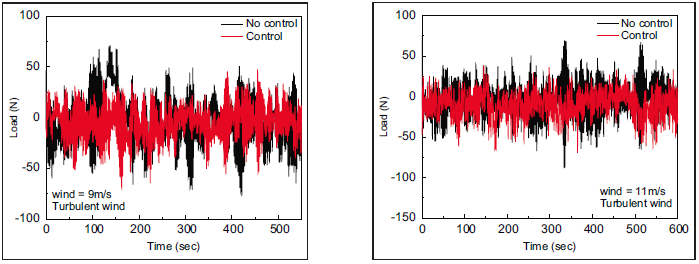
\includegraphics[scale=0.8]{tunnel.png}
\caption{The load variation in turbine blades has shown a decrease when controller was enabled at 9$ms^{-1}$ and 11$ms^{-1}$ airspeeds with gusting environments. \cite{lee}}
\centering
\end{figure}
\newline
This review of literature shows which areas have scope for improvement. It also shows the potential benefits of implementing such a control system. 
\section{Aims and objectives}
\thispagestyle{fancy}

The aim of the project is to design a control system that manages to suppress the rapid change in lift production as may be seen by the wing through a gust.
\newline
\newline
The control system should also be stable in steady conditions with no output disturbances. 
\newline
\newline
It should advance the settling time of the oscillation in lift in relation to an existing control system that settles an SPO in 0.263 seconds. The target is to settle the lift  within 50$\%$ of that time. 
\newline
\newline
The amplitude of the oscillation in lift should be smaller in the gust with the control system active than it would be without it. 
\newline
\newline
Lastly, first principles modelling will be used to determine the optimal PID gains and design the control system. Then, based on wind tunnel data heuristic techniques driven by collected data will be used to further improve the performance. Eventually, the controller will be manually tuned by trial and error to fine tune the controller gains. Comparing the gains determined by Simulink to the optimal gains determined by testing will verify whether the first principles model was valid. If not, the possible flaws in the model will be explored. This will be helpful for designing a control system for UAVs whose plants have not yet been constructed. 
\newline
\newline
In the next chapter, theory that can be applied to the project will be discussed. 
\newline
\newline
Then the instrumentation, equipment and the set up to facilitate measurement and data recording will be determined. 
\newline
\newline
Once the tools and equipment have been developed, the plant dynamics will be analysed in order to carry out simulations to obtain controller parameters. 
\newline
\newline
The implementation and the algorithm of the control program will need to be designed prior to testing. 
\newline
\newline
Finally, the control system will need to be tested in steady state conditions and in gusting environments and should clearly show that the control system manages to hold the lift at the setpoint.  




\thispagestyle{fancy}
\chapter{Theory}
\thispagestyle{fancy}
In this section, relevant theory that has been well established will be outlined. It may be helpful to first understand why SPOs occur and how control of wing lift can help solve the problem.  
\section{Flight dynamics}

This section will outline flight dynamics very briefly to help understand the mechanism of longitudinal dynamic modes such as a SPO.  

The longitudinal equations of motion can be used as a starting point :
\begin{multline}
\begin{bmatrix}\Delta\dot{u}\\\dot{w}\\\dot{q}\\\Delta\dot{\theta}\end{bmatrix} =
 \begin{bmatrix}\frac{\mathring{X}_{u}}{m}&\frac{\mathring{X}_{w}}{m}&0&-gcos\theta_{0}\\\frac{\mathring{Z}_{u}}{m-\mathring{Z}_{\dot{w}}}&\frac{\mathring{Z}_{w}}{m-\mathring{Z}_{\dot{w}}}&\frac{\mathring{Z}_{q}+mU_{\infty}}{m-\mathring{Z}_{\dot{w}}}&\frac{-mgsin\theta_{0}}{m-\mathring{Z}_{\dot{w}}}\\\frac{1}{I_{y}}\left[\mathring{M}_{u}+\frac{\mathring{M}_{\dot{w}}\mathring{Z_{u}}}{m-\mathring{Z}_{\dot{w}}}\right]&\frac{1}{I_{y}}\left[\mathring{M}_{w}+\frac{\mathring{M}_{\dot{w}}\mathring{Z_{u}}}{m-\mathring{Z}_{\dot{w}}}\right]&\frac{1}{I_{y}}\left[\mathring{M}_{q}+\frac{\mathring{M}_{\dot{w}}(\mathring{Z_{q}}+mU_{\infty})}{m-\mathring{Z}_{\dot{w}}}\right]&-\frac{M_{\dot{w}}mg\sin(\theta_{0})}{I_{y}(m-Z_{\dot{w}})}\\0&0&1&0\end{bmatrix}\begin{bmatrix}\Delta u\\w\\q\\\Delta\theta\end{bmatrix}+\\
\begin{bmatrix}\frac{\Delta \mathring{X_{c}}}{m}\\\frac{\Delta \mathring{Z_{c}}}{m-\mathring{Z}{\dot{w}}}\\\frac{\Delta \mathring{M}_{c}}{I_{y}} + \frac{\mathring{M}_{\dot{w}}}{I_{y}}\frac{\Delta \mathring{Z_{c}}}{m-\mathring{Z}{\dot{w}}}\\0\end{bmatrix}
\end{multline}


The derivations of these equations are fairly straightforward but quite lengthy and can be found in virtually any flight mechanics/dynamics textbook \cite{etkin}. The dynamics of flight (in the longitudinal direction) are heavily influenced by physical and geometric parameters such as the mass and the second moments of inertia around the y-axis (lateral direction) which influences the rotational kinematics of the aircraft. They are also influenced by the aerodynamic derivatives (e.g. $ \mathring{X}_{u,w}, \mathring{Z}_{u,w,q,\dot{w}}, \mathring{M}_{u,w,q,\dot{w}}$). 

These equations can be rewritten in the form:
\begin{equation}
\dot{\textbf{x}} = \textbf{Ax+B}
\end{equation}

Where $x$ is the state vector, $\textbf{A}$ is the system matrix (constant) and B is a vector of control forces and moments which can be considered 0.
\begin{equation}
\dot{\textbf{x}}=\textbf{Ax}
\end{equation}
This is a first order ODE which means that the solutions are in the form of
\begin{equation}
\textbf{x}=\textbf{x}_{0}e^{\lambda t}
\end{equation}
\begin{equation}
\lambda\textbf{x}_{0}=\textbf{Ax}_{0}
\end{equation}
\begin{equation}
(\textbf{A}-\lambda\textbf{I})\textbf{x}_{0}=0
\end{equation}

Non-trivial solutions occur when $det(\textbf{A}-\lambda\textbf{I})=0$. Solving this equation for any given aircraft will give a quartic equation (4th order polynomial) which when solved will give two pairs of complex conjugates. One of the pairs corresponds to the phugoid mode while the other one corresponds to the SPO. 

For example, consider the Navion aircraft \cite{navion}:
\begin{equation}
\textbf{A} = \begin{bmatrix}
-0.09148&0.04242&0&-32.17\\
10.51&-3.066&152&0\\
0.2054&-0.05581&-2.114&0\\
0&0&1&0
\end{bmatrix}
\end{equation}

Computing the eigenvalue of this matrix:
\begin{figure}[H]

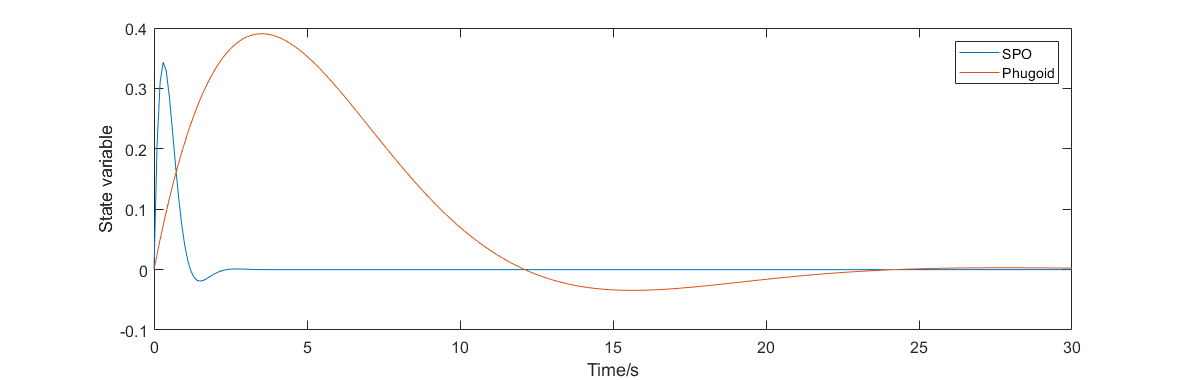
\includegraphics[width=1\textwidth,left]{DI.png}
\caption{Graph showing how the state variable (pitch rate) changes with time in SPO (blue line) and phugoid (orange line) modes. }

\end{figure}
The matrix produces two pairs of complex conjugate eigenvalues. The first pair $\lambda_{1,2}= -2.4352 \pm 2.6461i$ is the SPO mode. The decay rate (the real part) is much greater than the other pair $\lambda_{3,4} = -0.2006 \pm 0.2593i$ and so is the frequency (coefficient of i). 
\subsection{The relevance to control of wing lift}
The control vector \textbf{B} was assumed to be 0 here. In other words, this only applies if no control forces are applied. However, when the control system is active, vector \textbf{B} will not be 0. The controller will adjust this vector (specifically the third element) in order to oppose any disturbance including a dynamic mode. From equation 2.1, it can be seen that the aerodynamic derivatives relating to the pitching moment on the aircraft affect the pitch rate ($\dot{q}$). Pitching moment is influenced mostly by the aerodynamic contributions from the wing and the tailplane. Thus, controlling lift is a way of mitigating longitudinal dynamic modes.   


Controlling dynamic modes as opposed to the lift is still different because the former implies a flight test. It can be difficult to test a control system directly on an aircraft because flight tests are more expensive, more complicated to run and pose some health and safety risks. It will be much more convenient, safer and quicker to run wind tunnel tests first. Therefore, the system will not be tested in an actual SPO but through a gust (which can induce a SPO). However, it is safe to assume that if the wing lift is being damped by the control system, a SPO will be suppressed during flight because the change in pitch angle is a result of the increased wing lift as discussed above. 
\thispagestyle{fancy}
\section{SPO regulations and qualification}
By considering the laws that determine whether the SPO of an aircraft is acceptable can help explain why there has been little development in control systems that try to reject gusts. 

 
The United States of America's Federal Aviation Authority regulates SPOs in FAR Part 23.181 \cite{far} as follows:
Any short period oscillation not including combined lateral-directional oscillations occurring between the stalling speed and the maximum allowable speed appropriate to the configuration of the airplane must be heavily damped with the primary controls -

(1) Free; and

(2) In a fixed position.
\newline
United Kingdom's Civil Aviation Authority regulates SPOs in a very similar manner and can be found in CAP482 S181. 


The quality of handling is largely determined by pilot opinion. Pilot opinion is collected and visualised on "opinion contours" which take the undamped natural frequency and the damping ratio into account. These parameters need to be adjusted until the pilot finds the controls satisfactory. 


These parameters (natural frequency and damping ratio) determine whether an aircraft's SPO qualifies and also whether the controls are satisfactory to the pilot. 
\begin{figure}[H]
\centering
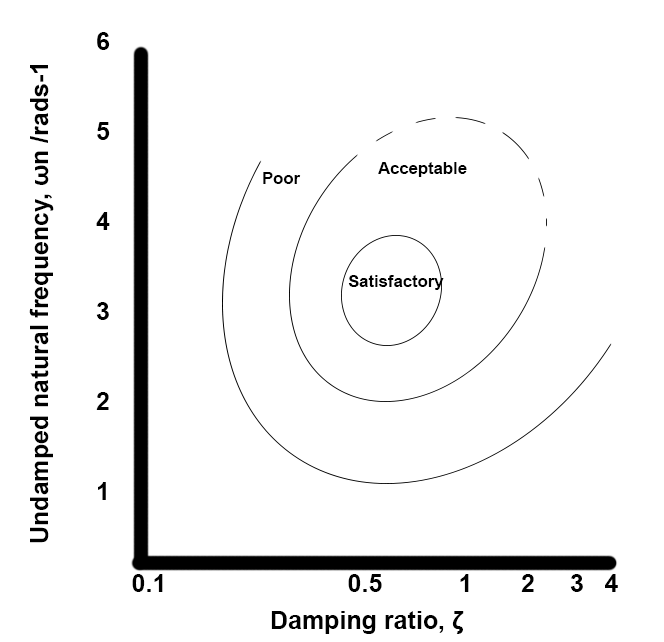
\includegraphics[width=0.6\textwidth,center]{conto.png}
\caption{Sketch illustrating what a pilot opinion contour might look like. The goal is to adjust the damping ratio and the natural frequency to bring the opinion in the 'satisfactory' region.}
\centering
\end{figure}
From SPO approximation \cite{short} the natural frequency and damping ratio can be determined:
\begin{equation}
\omega_{n}=\sqrt{\mathring{Z}_{w}\mathring{M}_{q}+\mathring{M}_{w}\mathring{Z}_{q}}
\end{equation}
\begin{equation}
\zeta = \frac{\mathring{M}_{q}+\mathring{Z}_{w}}{\omega_{n}}
\end{equation}

Therefore, simply by adjusting the aerodynamic derivatives, it is possible to conform to the regulations and to improve the pilot opinions. The regulations do not make the existence of a control system with a SPO dedicated model mandatory. This may explain the lack of development in this field.
\thispagestyle{fancy}
\section{Trailing edge flap}
\thispagestyle{fancy}
The last section established the need for a mechanism that can control wing lift. Flaps are typically used as high-lift devices deployed in conditions where the airspeed is low. Increased lift is desirable to minimise the distance to take off or to achieve slower and steeper approaches during landing because extending flaps will lower the stall speed of the aircraft. The principle of operation is quite straightforward. Deploying the flap will increase the $C_{L}$ and deflecting it upwards will decrease it. This in turn will change the lift produced as per the lift equation: 
\begin{equation}
L=\frac{1}{2} \rho V^{2} SC_{L}
\end{equation}


For a plain flap, the increase in lift can also be understood by realising that the airspeed under the wing will be slowed down when the flap is deflected downwards. Therefore, some of the dynamic pressure will be converted to static pressure increasing the pressure under the wing and consequently the lift. Deflecting the flap upwards will have the  opposite effect: the speed at the top of the of the airfoil will be slowed down which will increase the static pressure here. This increased pressure acts opposite to the direction of positive lift and thus will reduce the size of the lift or it could produce negative lift. 

A plain flap can both increase and decrease lift which will be useful to regulate lift through a gust. 


\section{PID controller}
\thispagestyle{fancy}
A mechanism has been decided to control the lift at different airspeeds. However, a command signal needs to generated to set the flap angle. A PID controller could do this task. 


While a PID controller (or it's variations) is not the only controller in existence, it is by far the most commonly used controller in industrial applications. The reason for it's popularity is most likely because it is easy to implement and gives the user the ability to fine tune the performance of the control system. For example, if the user desires a fast but less robust (allows overshoot) system, he/she can increase the integral gain. 

By adjusting the gains, you can change the rise time, peak time, settling time, percentage overshoot and the steady state error (if applicable). 

A PID output is the sum of the proportional, integral and derivative outputs. The proportional output is proportional to the error. The integral output is proportional to the integral of the error with respect to time. And finally, the derivative output is proportional to the rate of change of error. The following equation describes the output of a PID controller in the time domain. 
\begin{equation}
output = K_{p}e(t)+K_{i}\int e(t) dt+K_{d}\frac{de(t)}{dt}
\end{equation}
\thispagestyle{fancy}
Or in the laplace domain:
\begin{equation}
\mathcal{L}[output]=K_{p}+\frac{K_{i}}{s}+K_{d}s
\end{equation}
The essential theory applicable to this project has now been established. The next step would be designing the instrumentation for a feedback controller. 


\chapter{Instrumentation}
The theory required for the project has now been identified. To commence the project, the first task was to design and build the instrumentation required to measure and record the data. The computer and the programming language determines how the controller will be implemented. The sensing equipment and data processing are also very important factors because the quality of the data relies on them. 

 
\thispagestyle{fancy}
\section{Computer and programming language}
\thispagestyle{fancy}
At the moment, there are two major options for an embedded system: Arduino and Raspberry Pi. 
\newline
\newline
The Arduino Mega uses an Atmel ATmega 2560 processor with a clock speed of 16MHz. The program for the Arduino is written in a subset of the C/C++ programming language on a desktop computer and copied to the onboard flash memory over USB typically. The Arduino IDE can be used to compile and write the executable to the flash memory. It also allows for serial communication with the device which is useful for debugging. 
\newline
\newline
The Raspberry Pi 3 has a 4-core 1.2GHz Broadcom BCM2837 64bit CPU running at 1.2 GHz which is much faster than the Arduino Mega. The extra processing power allows the user to use the Raspberry Pi as a full fledged computer. The programs can even be written on the device itself. However, it will be easier to program on a desktop and push the code to the Raspberry Pi over WiFi using the Secure Shell (SSH) protocol. 
\newline
\newline
\begin{figure}[H]
\centering
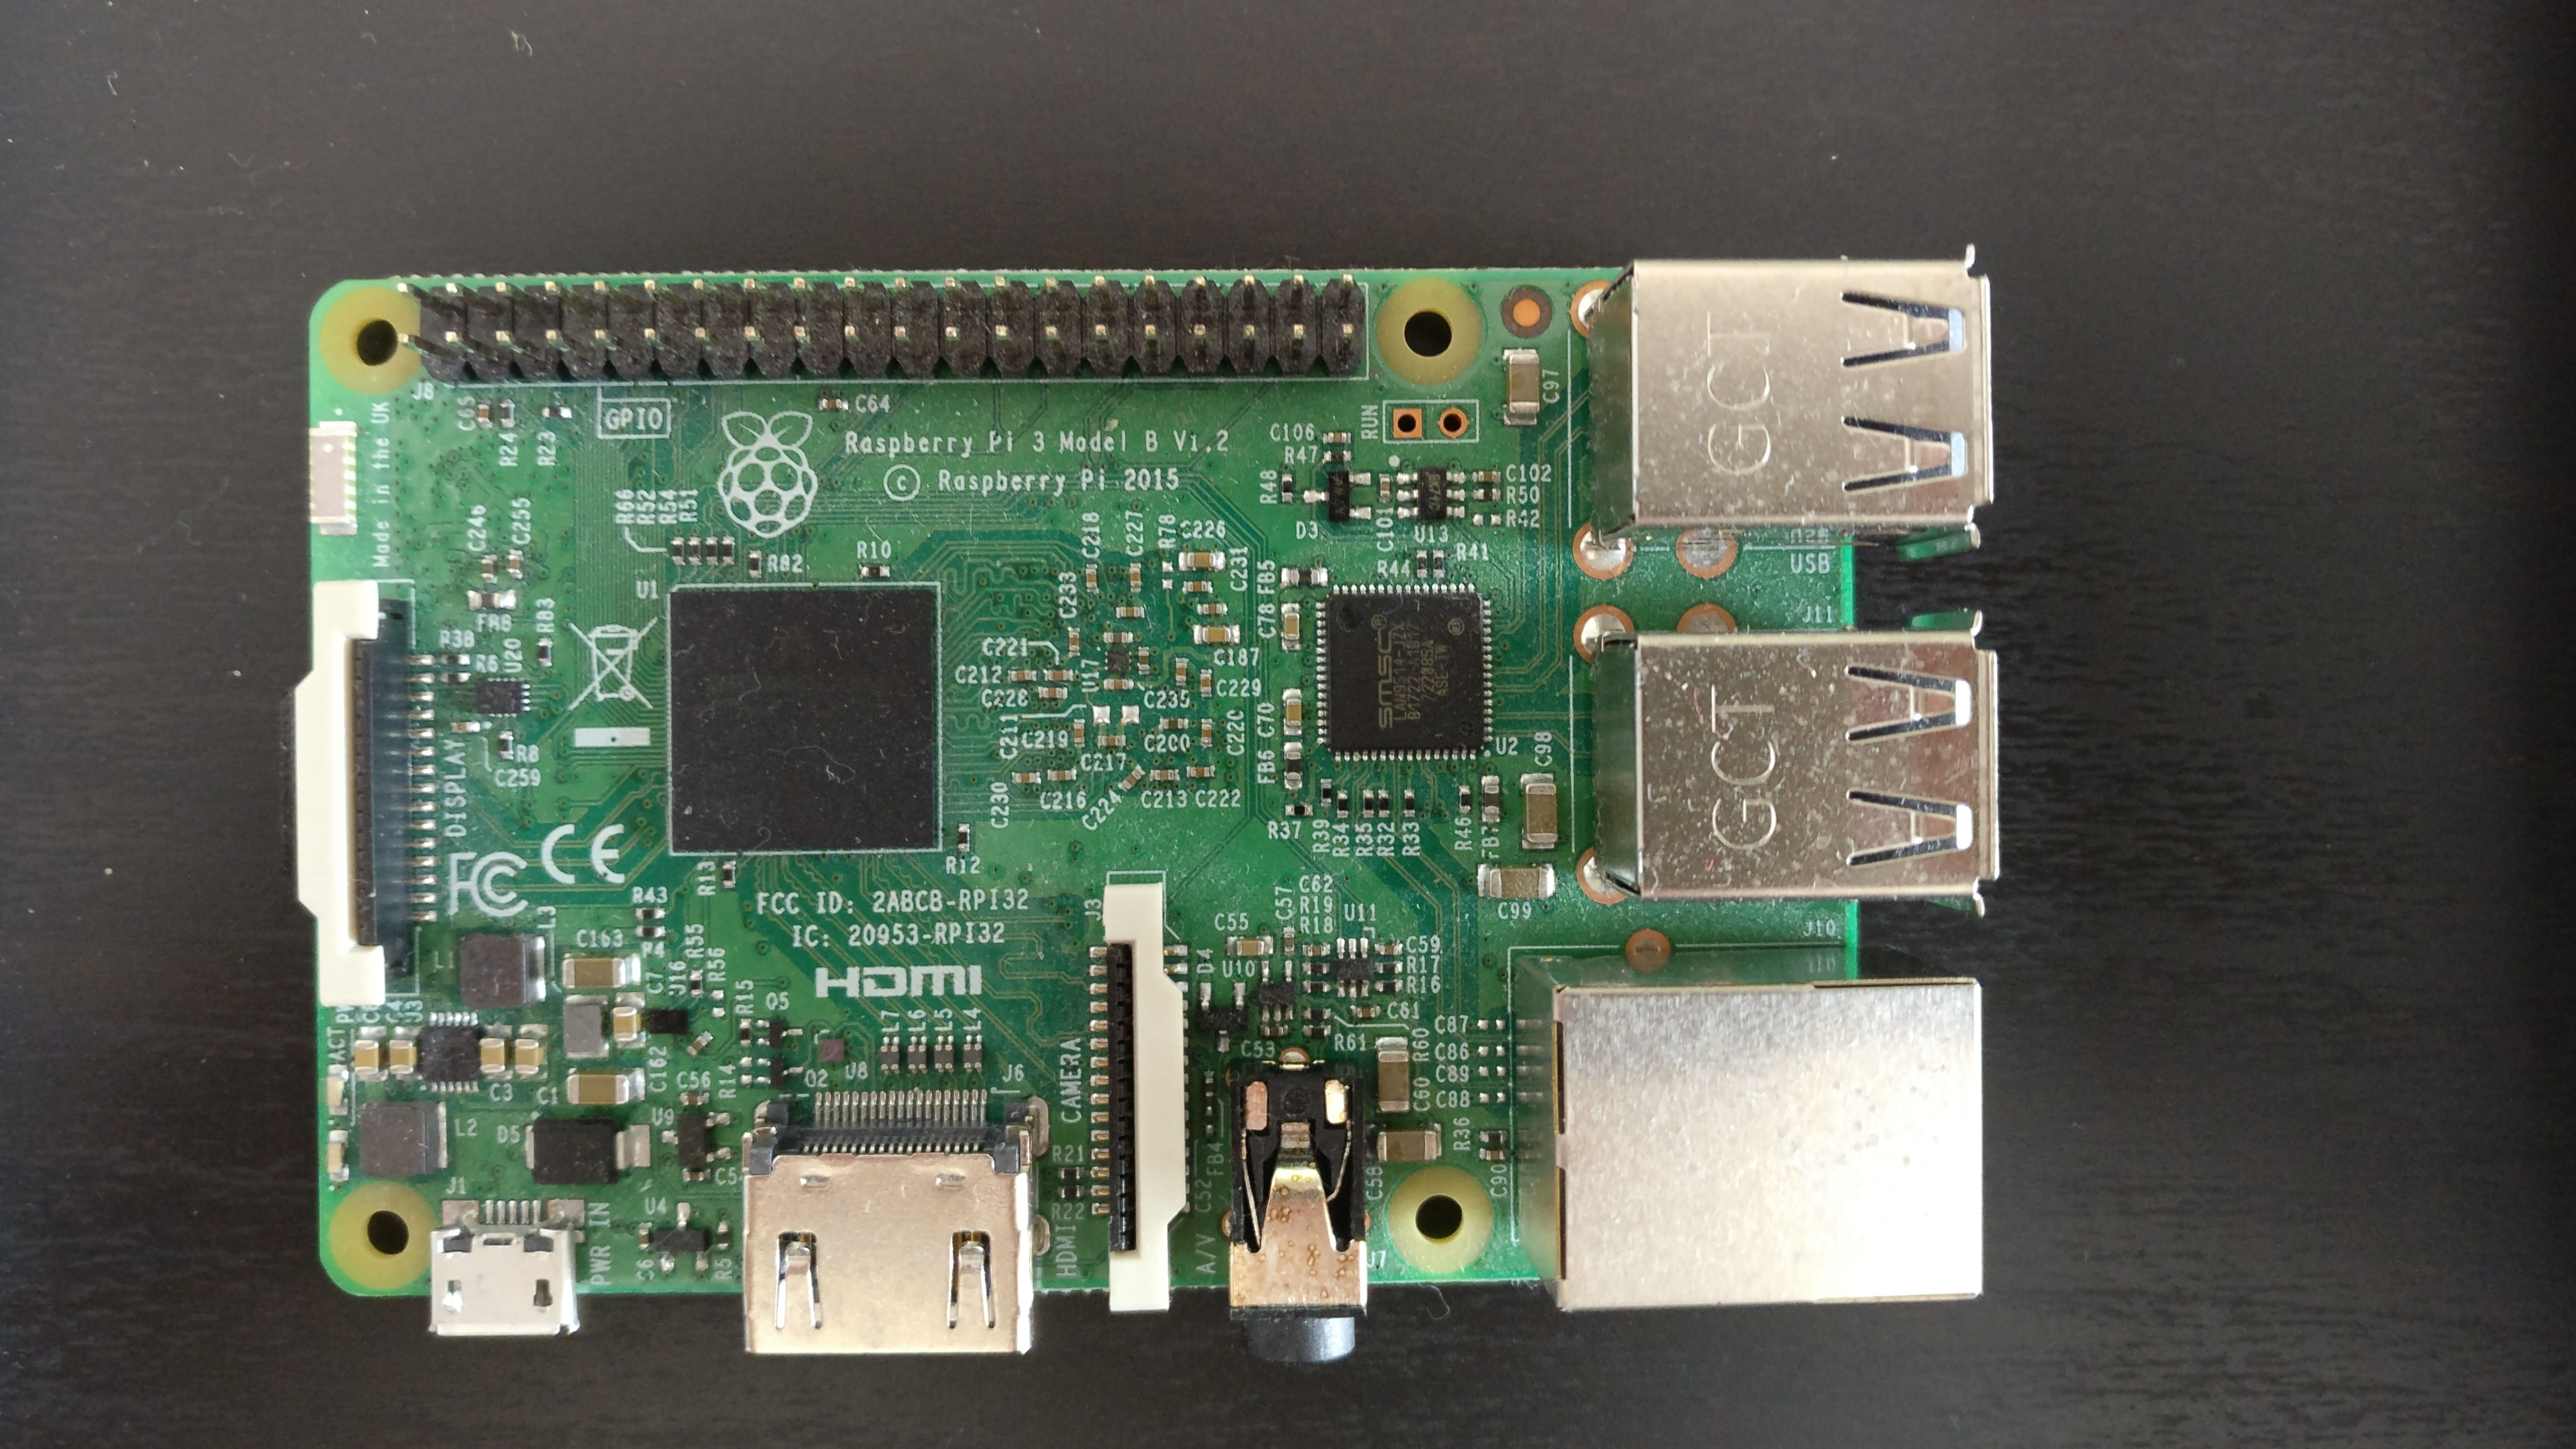
\includegraphics[scale=0.05]{rpi.jpg}
\caption{The Raspberry Pi 3 Model B microcontroller}
\end{figure}
The Raspberry Pi also gives the user a choice of programming languages to use unlike the Arduino. Python is most commonly used to code for the Raspberry Pi. However, it would be more suitable to use a compiled language like C/C++ rather than an interpreted language like Python. While C can be difficult and more time consuming than Python to write and debug, it does run faster. The table below \cite{comp} shows the results from a Mandelbrot Set test (a recursive algorithm) for Python 3 and C++ with the g++ compiler. 
\newline
\newline
$\begin{array}{ | l | l | l | l | l | l | l | }
\hline
\centering
	 source & secs & mem & gz & cpu & cpu load \\ \hline
	 Python 3 & 225.24 & 15736 & 688 & 899.25 & 100\% 100\% 100\% 100\% \\ \hline
	 C++ g++ & 1.64 & 27636 & 1002 & 6.51 & 100\% 99\% 100\% 99\% \\ \hline
\end{array}$
\newline
\newline
Speed is of the essence in this project since the objective is to minimise the rise times and settling times. Thus C++ executed on the Raspberry Pi 3 is the most suitable option.  
\section{Pressure sensors}
This is one of the most important design decision for this project because they determine the ability to detect a change in airflow and lift (process variable) which is essential for a closed-loop feedback system.

There are a variety of sensors to choose from. There are absolute pressure sensors that simply measure the gauge or absolute pressure of air at a single point. Then there are pressure sensors that measure differential pressure. These have two ports and the sensor will measure the difference in pressure the two ports are subjected to. 

To calculate the lift on the wing, the pressure distribution along the top and the bottom of the wing will be measured. A single differential pressure sensor can tell the difference in pressure at the top and bottom of a wing at a certain chord position. For the same information, two absolute pressure sensors will be required. Furthermore, the airspeed in the wind tunnel will need to be measured. Using a differential sensor, one port can be subjected to the total/stagnation pressure from a pitot probe, and the second port will be subjected to the static pressure. The sensor will instantly give the difference between the two pressures which is the dynamic pressure. The airspeed can then be easily calculated using Bernoulli's principle:
\thispagestyle{fancy} 
\begin{equation}
V=\sqrt{\frac{2(p_{0}-p)}{\rho}}
\end{equation}
Thus, for convenience a differential type sensor will be used. TE connectivity makes a sensor called MS4524DO in both differential and absolute types. There is also the option to choose between the I2C and SPI data transmission buses. 
\thispagestyle{fancy} 
There are merits to using both buses. The I2C bus is very common and many devices use it to communicate with a 'master'. The bus typically runs at 100kbps but can reach 400kbps on fast mode. It uses a data line (SDA) and a clock line (SCL) and is therefore sometimes called 'two wire interface' (TWI). 

SPI on the other hand runs much faster at around 10Mbps. The interface requires a clock line (SCLK), a MISO line (Master in Slave out), sometimes a MOSI line (Master out Slave in) and a slave select pin. 

The slave select pin allows communication with a specific device on the line. In this case, four pressure sensors are used but only one sensor can be communicated with at once. So data from consecutive sensors will be acquired sequentially. 

I2C relies on the device address. Each I2C device is given a specific address which needs to be provided before data transmission can happen. All available I2C MS4525DO sensors have the address 0x28 which creates a conflict. The I2C bus will not know which sensor to communicate with because they're all at the same address. A 'switching' mechanism will be needed to make this option viable.

The most suitable bus for this application is obviously SPI. However, there is a severe lack of availability of these sensors at a reasonable price. A compromise in speed had to be made by choosing the I2C sensor which are widely available. However, for my purpose the speed exceeds Nyquist criterion (test described in section 3.4) so the lower bus speed will not be an issue.

\section{Electronic setup}
\thispagestyle{fancy}
\begin{figure}[H]
\centering
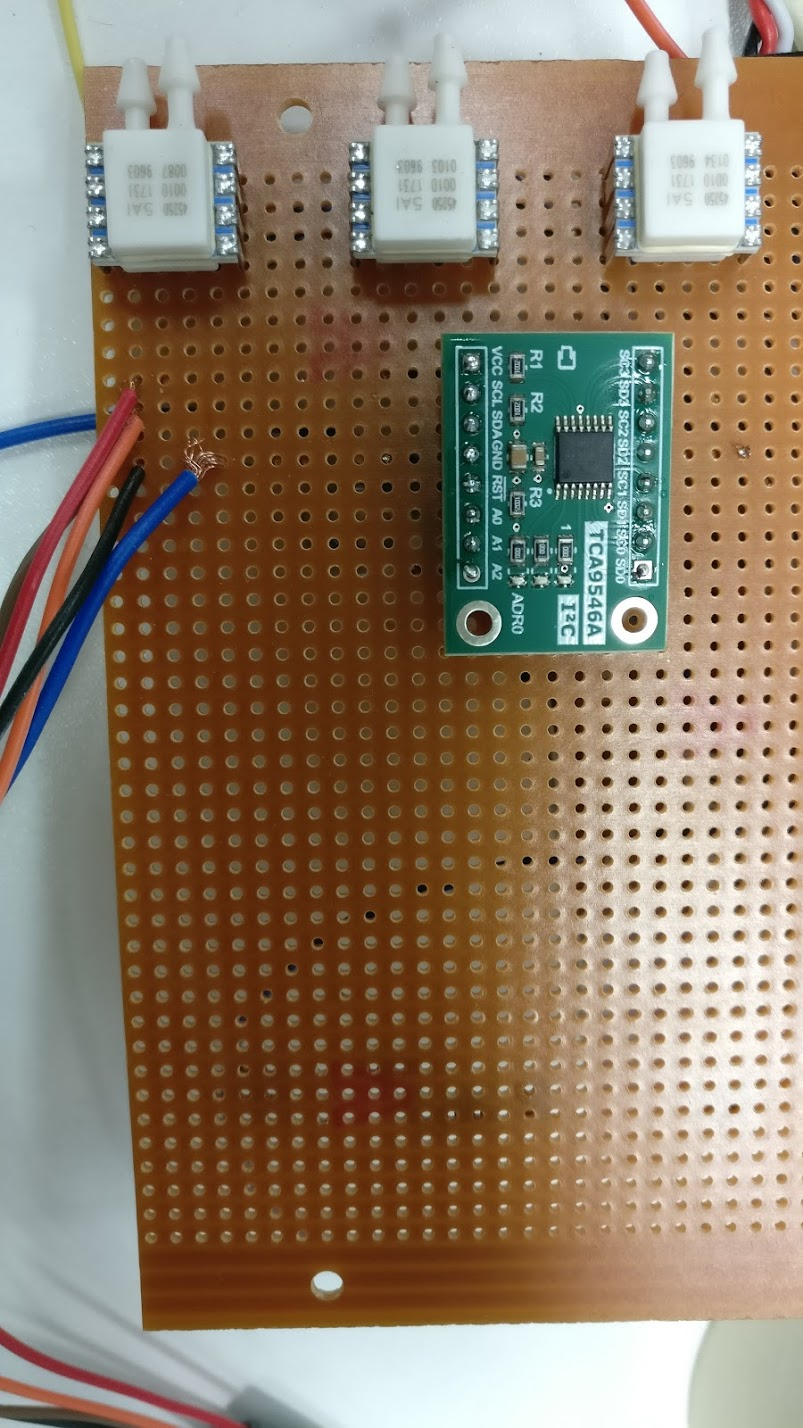
\includegraphics[scale=0.15]{elec.jpg}
\caption{Photo of the breadboard with the multiplexer and the pressure sensors}
\centering
\end{figure}
As mentioned above, the I2C pressure sensors all have the same address so are bound to create a conflict unless a switching mechanism is constructed. An I2C multiplexer called TCA9546a which is an I2C device itself was used. 

It has four channels thus can handle four I2C devices. To select a channel, a number is sent to the I2C address 0x77 (where the multiplexer is located). 
\begin{table}[H]
\label{my-label}
\begin{tabular}{lll}
Channel 0 & 0x01     \\
Channel 1 & 0x02      \\
Channel 2 & 0x04		\\
Channel 3 & 0x08
\end{tabular}
\end{table}
\thispagestyle{fancy}
\begin{sidewaysfigure}
\centering
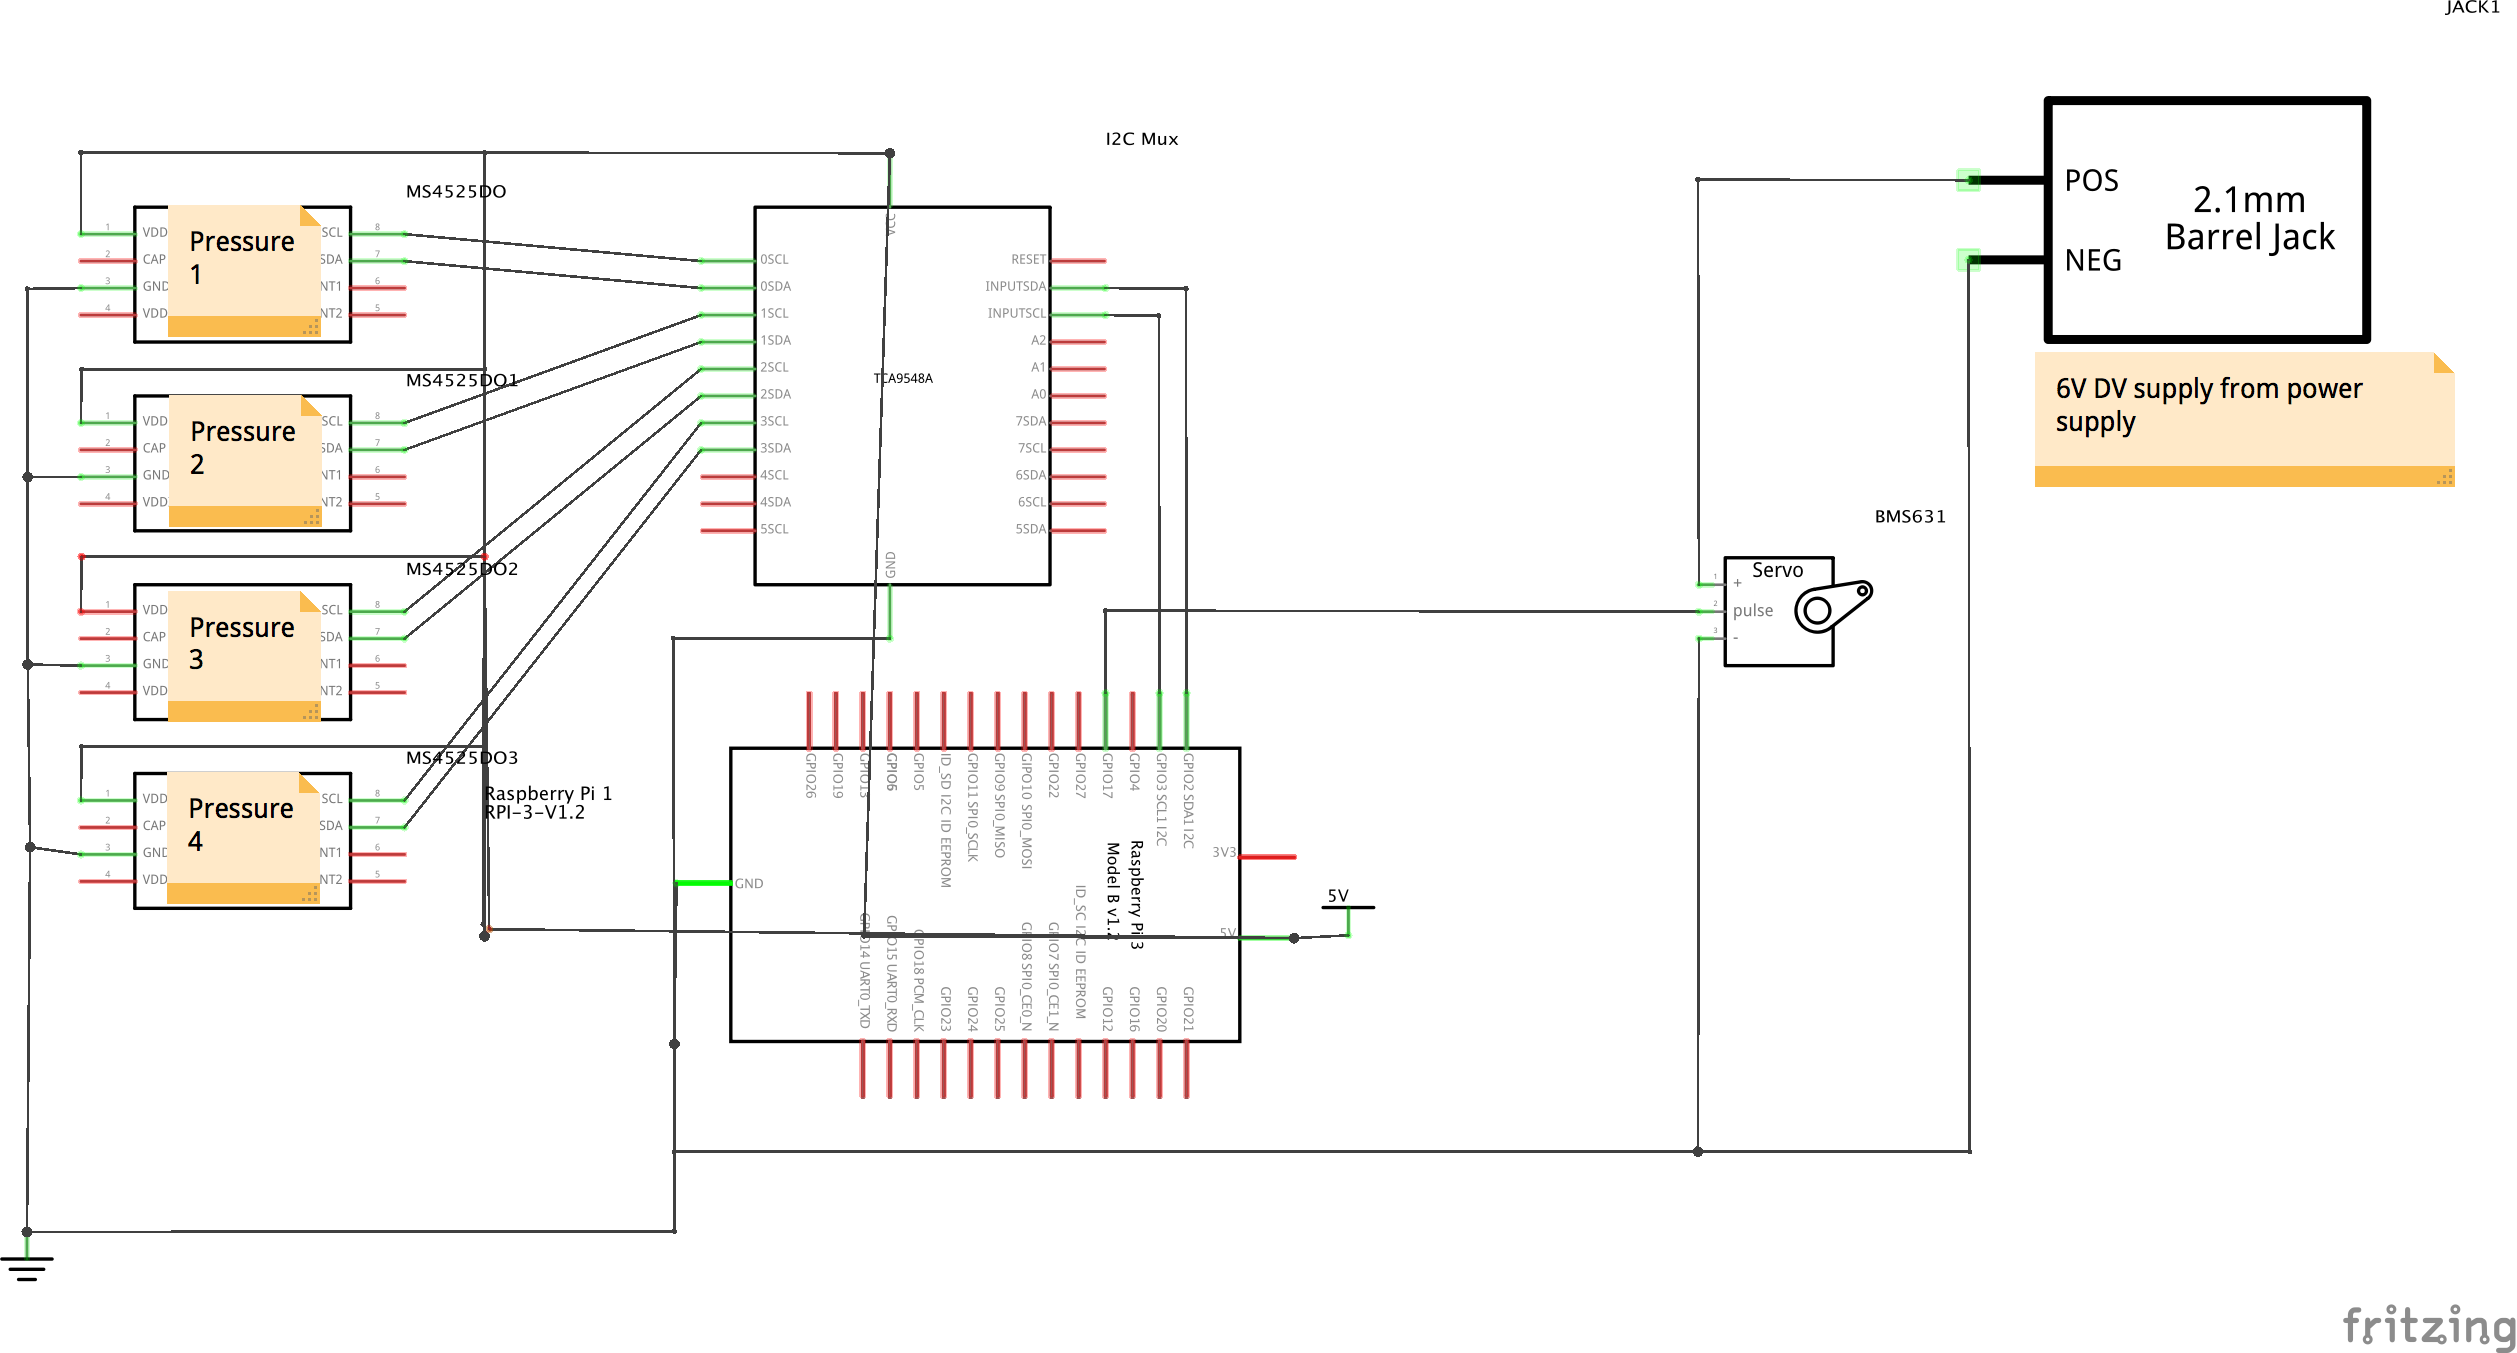
\includegraphics[scale=1]{ip.png}
\caption{Fritzing diagram illustrating the electronic set up. Note that the servo is powered externally via a 6V DC wall adapter, but the ground of the external power source and the Raspberry Pi power source are tied together because the servo and the Raspberry Pi need a common ground.}
\centering
\end{sidewaysfigure}
\thispagestyle{fancy}


Once the channel is selected, I2C communication between the Raspberry Pi and the selected pressure sensor can begin. Figure 3.3 on the next page illustrates the connection between the multiplexer and the pressure sensors. 



\newpage
\section{Sensor calibration}
\thispagestyle{fancy} 
The pressure sensors need to be calibrated against known values of pressures before they can be used. To achieve this, principles of a manometer were used. The difference in pressure heads at the two ends of the tube is proportional to the difference in pressure.
\begin{equation}
\Delta P = \rho_{w} g \Delta h
\end{equation}
\begin{figure}[H]
\centering
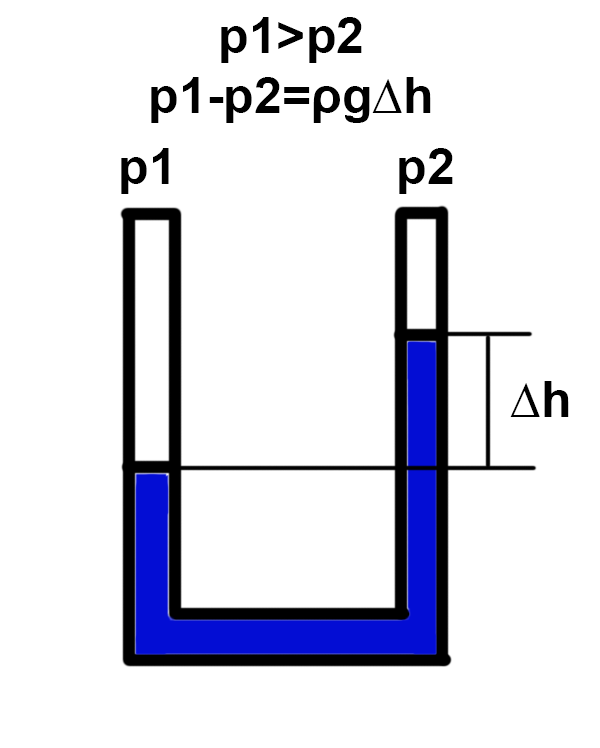
\includegraphics[width=0.5\textwidth,center]{mano.png}
\caption{Diagram illustrating principle of manometer and how the fluid level changes when the ends are subjected to different pressures \cite{jd}}
\centering
\end{figure}
Height differences of -10cm,-5cm,0cm,5cm and 10cm were created by raising the level of water in a PVC tube. Both ends were connected to the ports of the sensors to give pressure differentials of $0 Pa$, $\pm 490.5 Pa$ and $\pm 981 Pa$. The pressure sensors output the number of decimal counts. Results were collected for each sensor and are plotted below. These allowed me to convert the sensor output to pressure in pascals. The test results are shown in the figure 3.5 overleaf. 
\begin{figure}[H]
\centering
\subfloat{%
\resizebox*{8cm}{!}{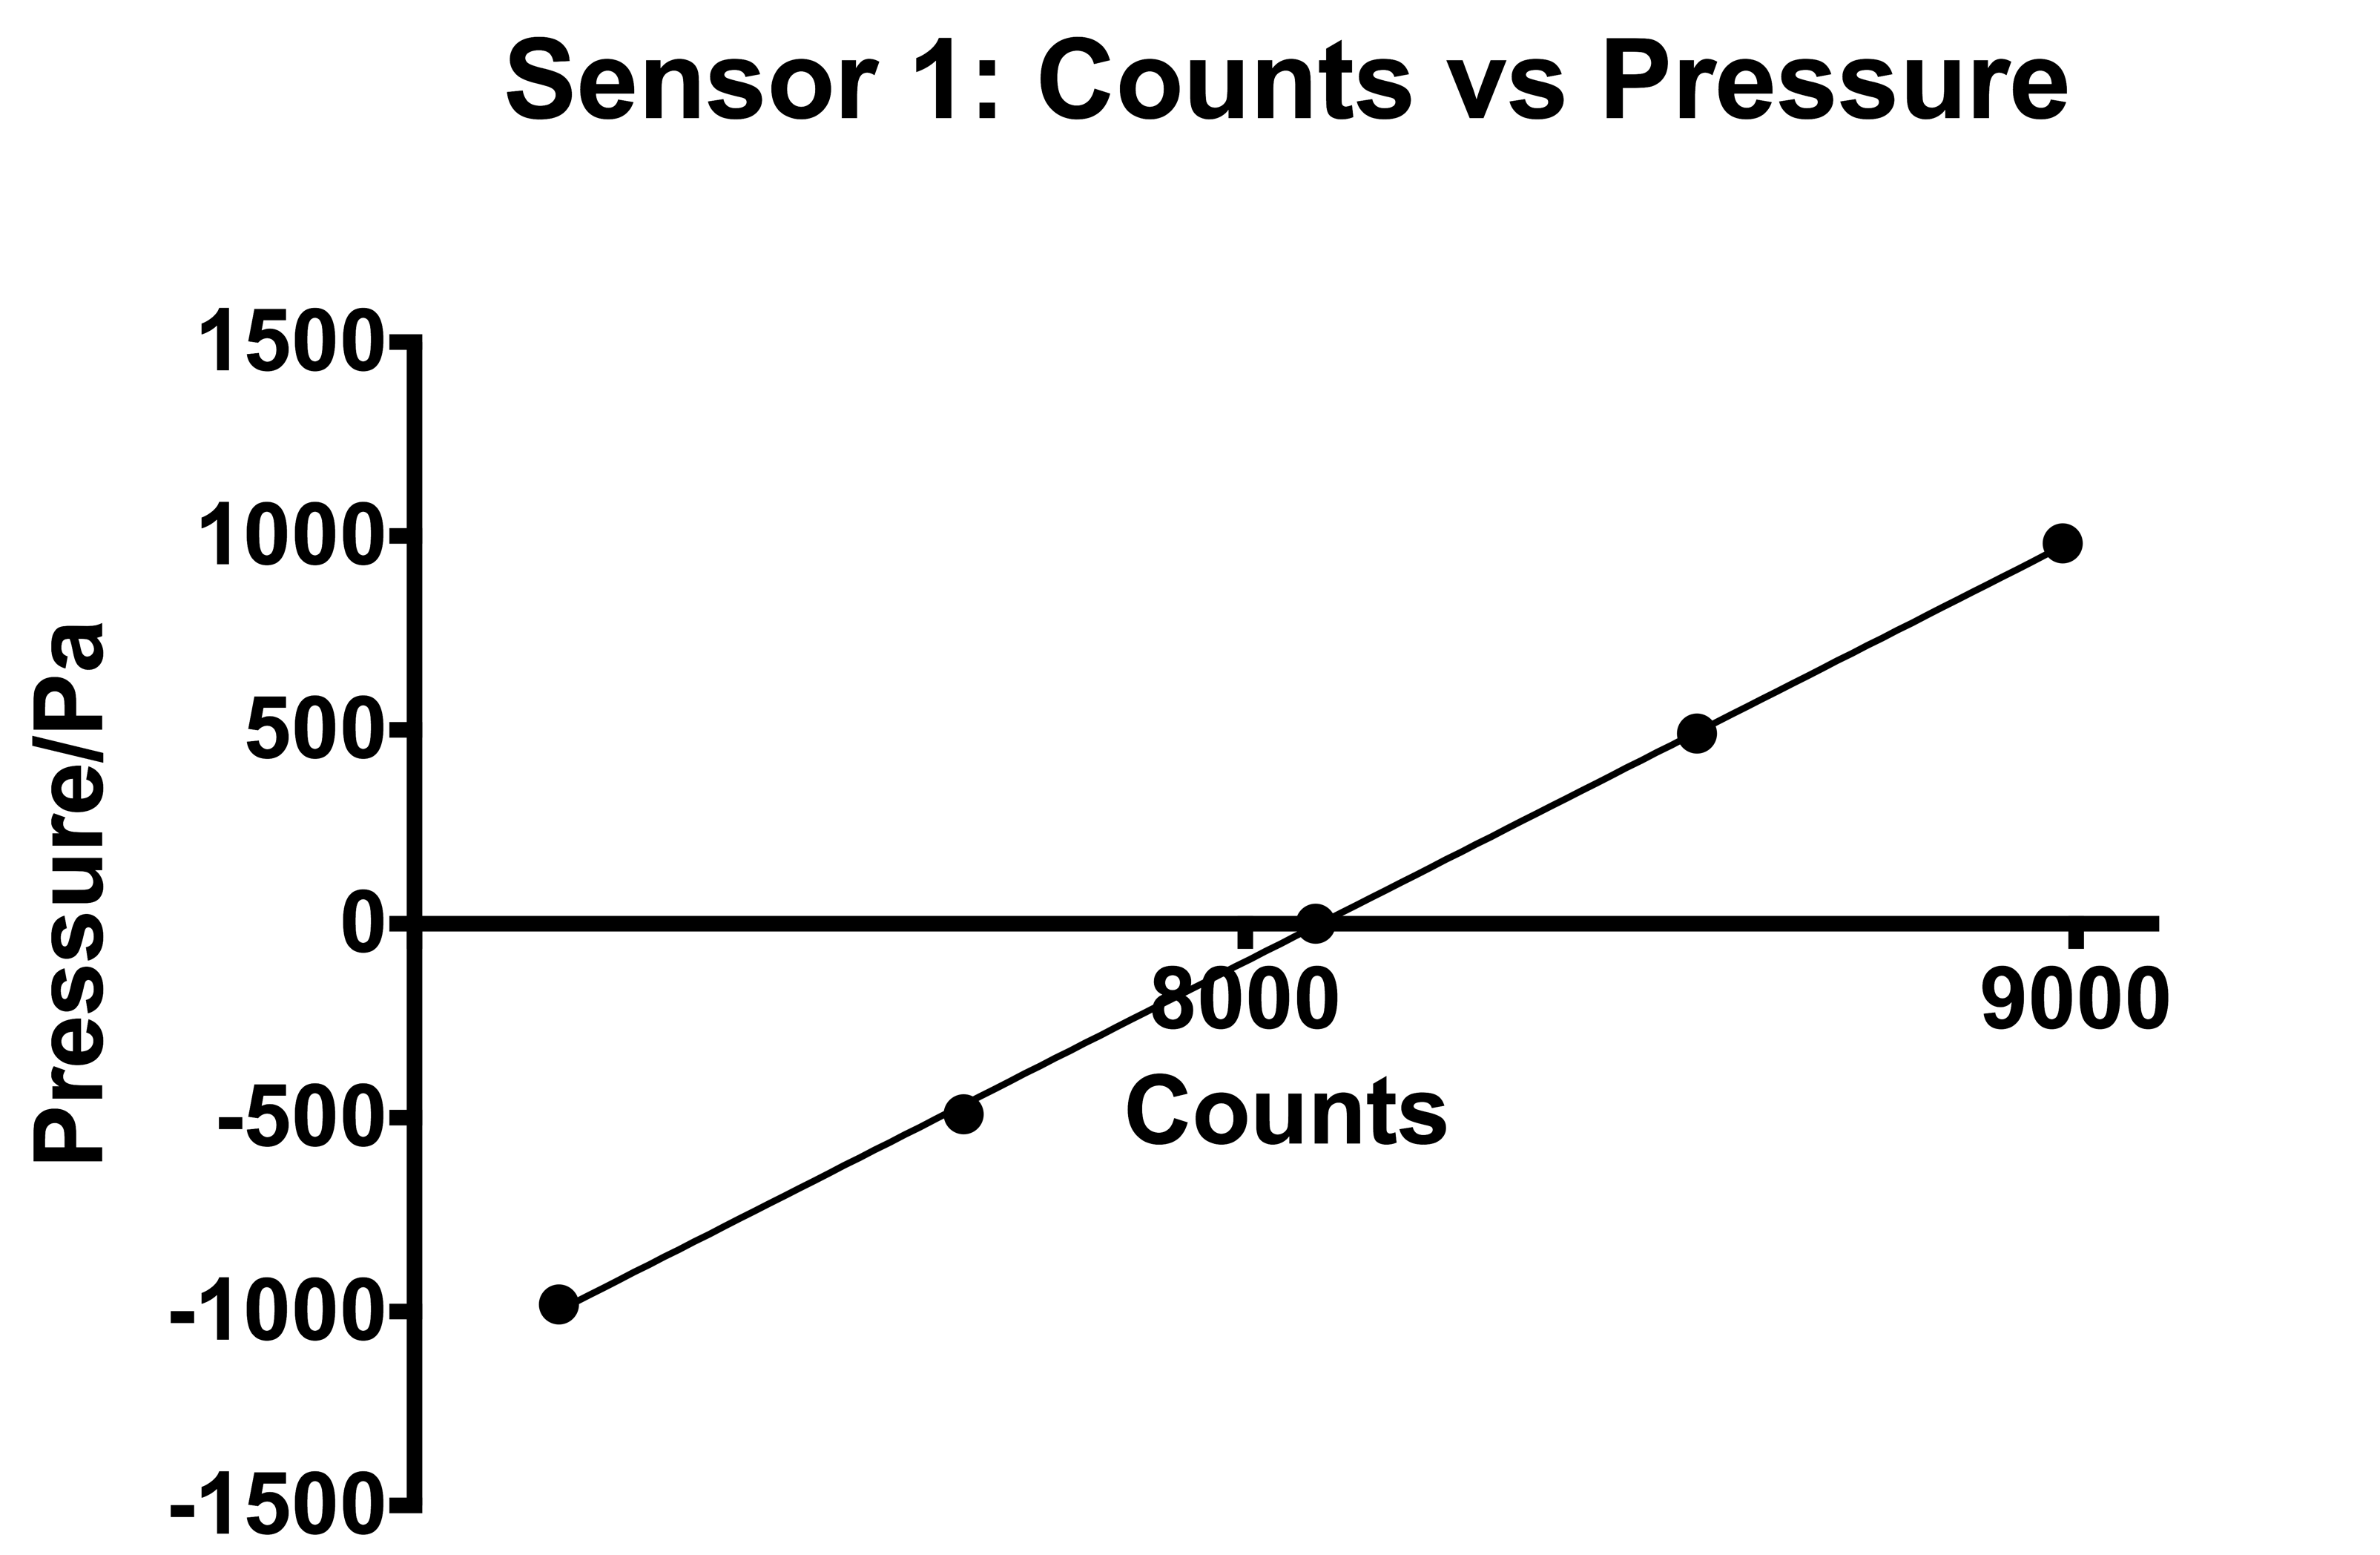
\includegraphics{s1.png}}}\hspace{5pt}
\subfloat{%
\resizebox*{8cm}{!}{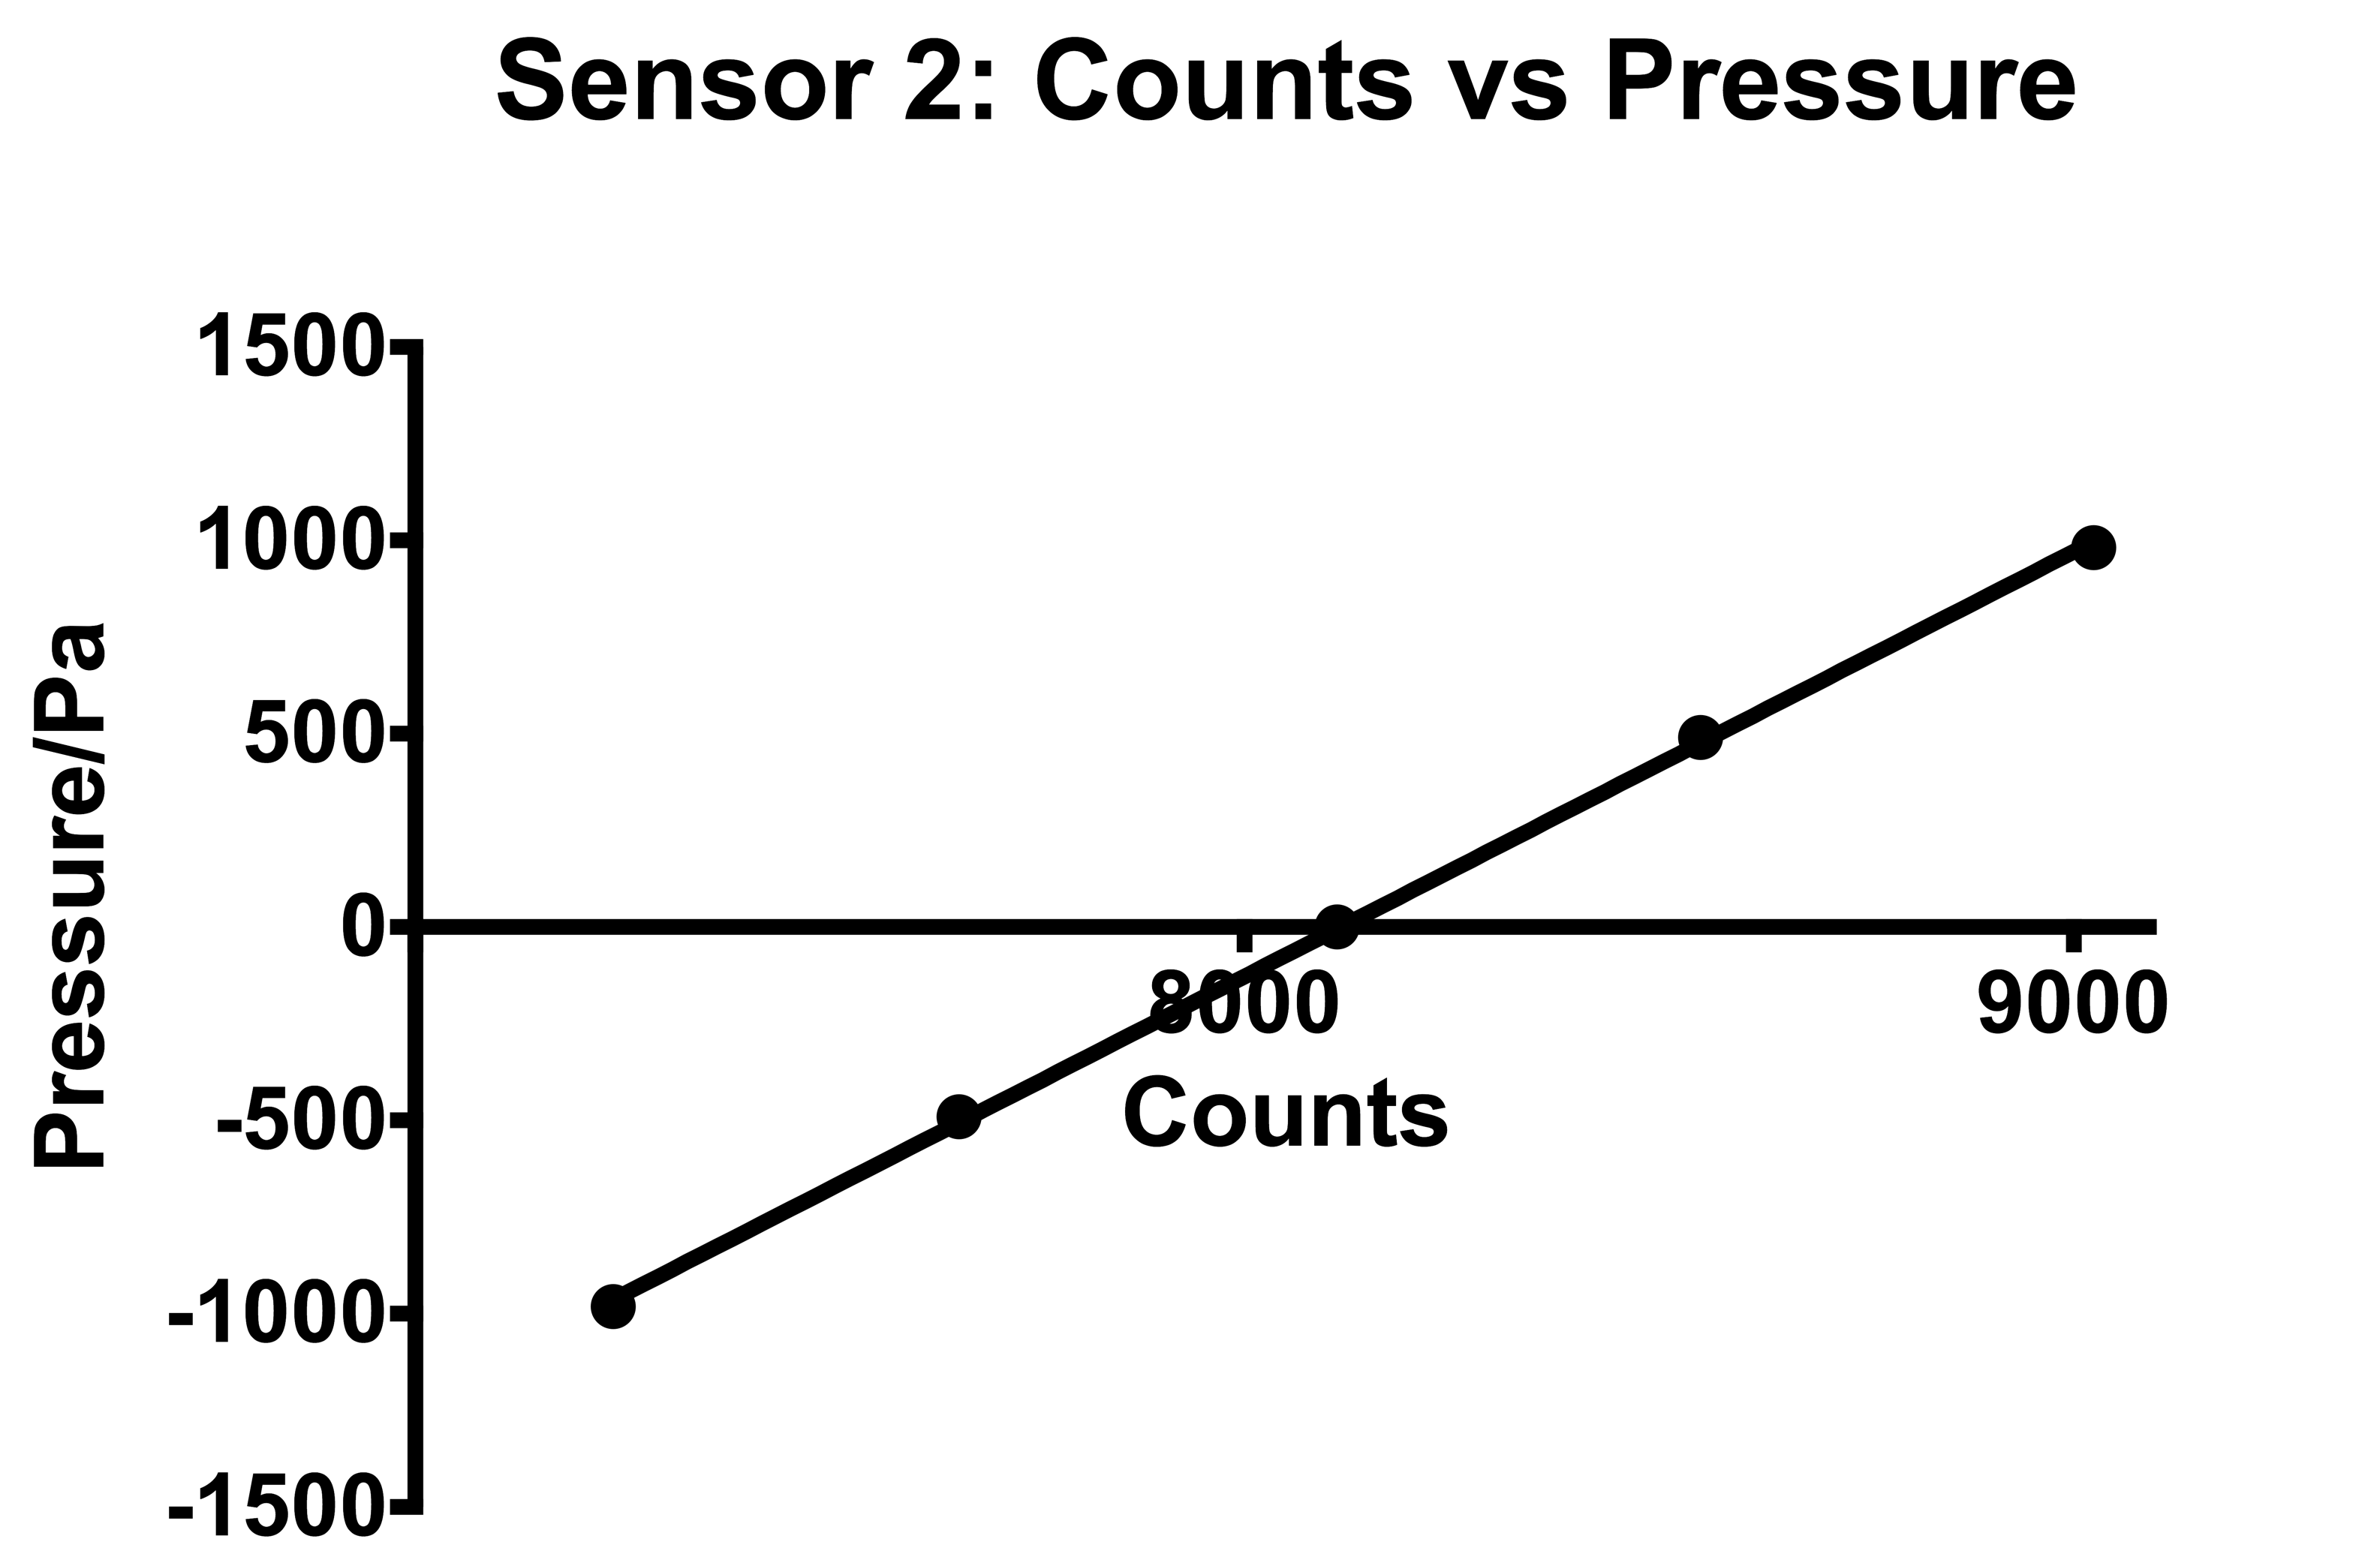
\includegraphics{s2.png}}}\hspace{5pt}
\subfloat{%
\resizebox*{8cm}{!}{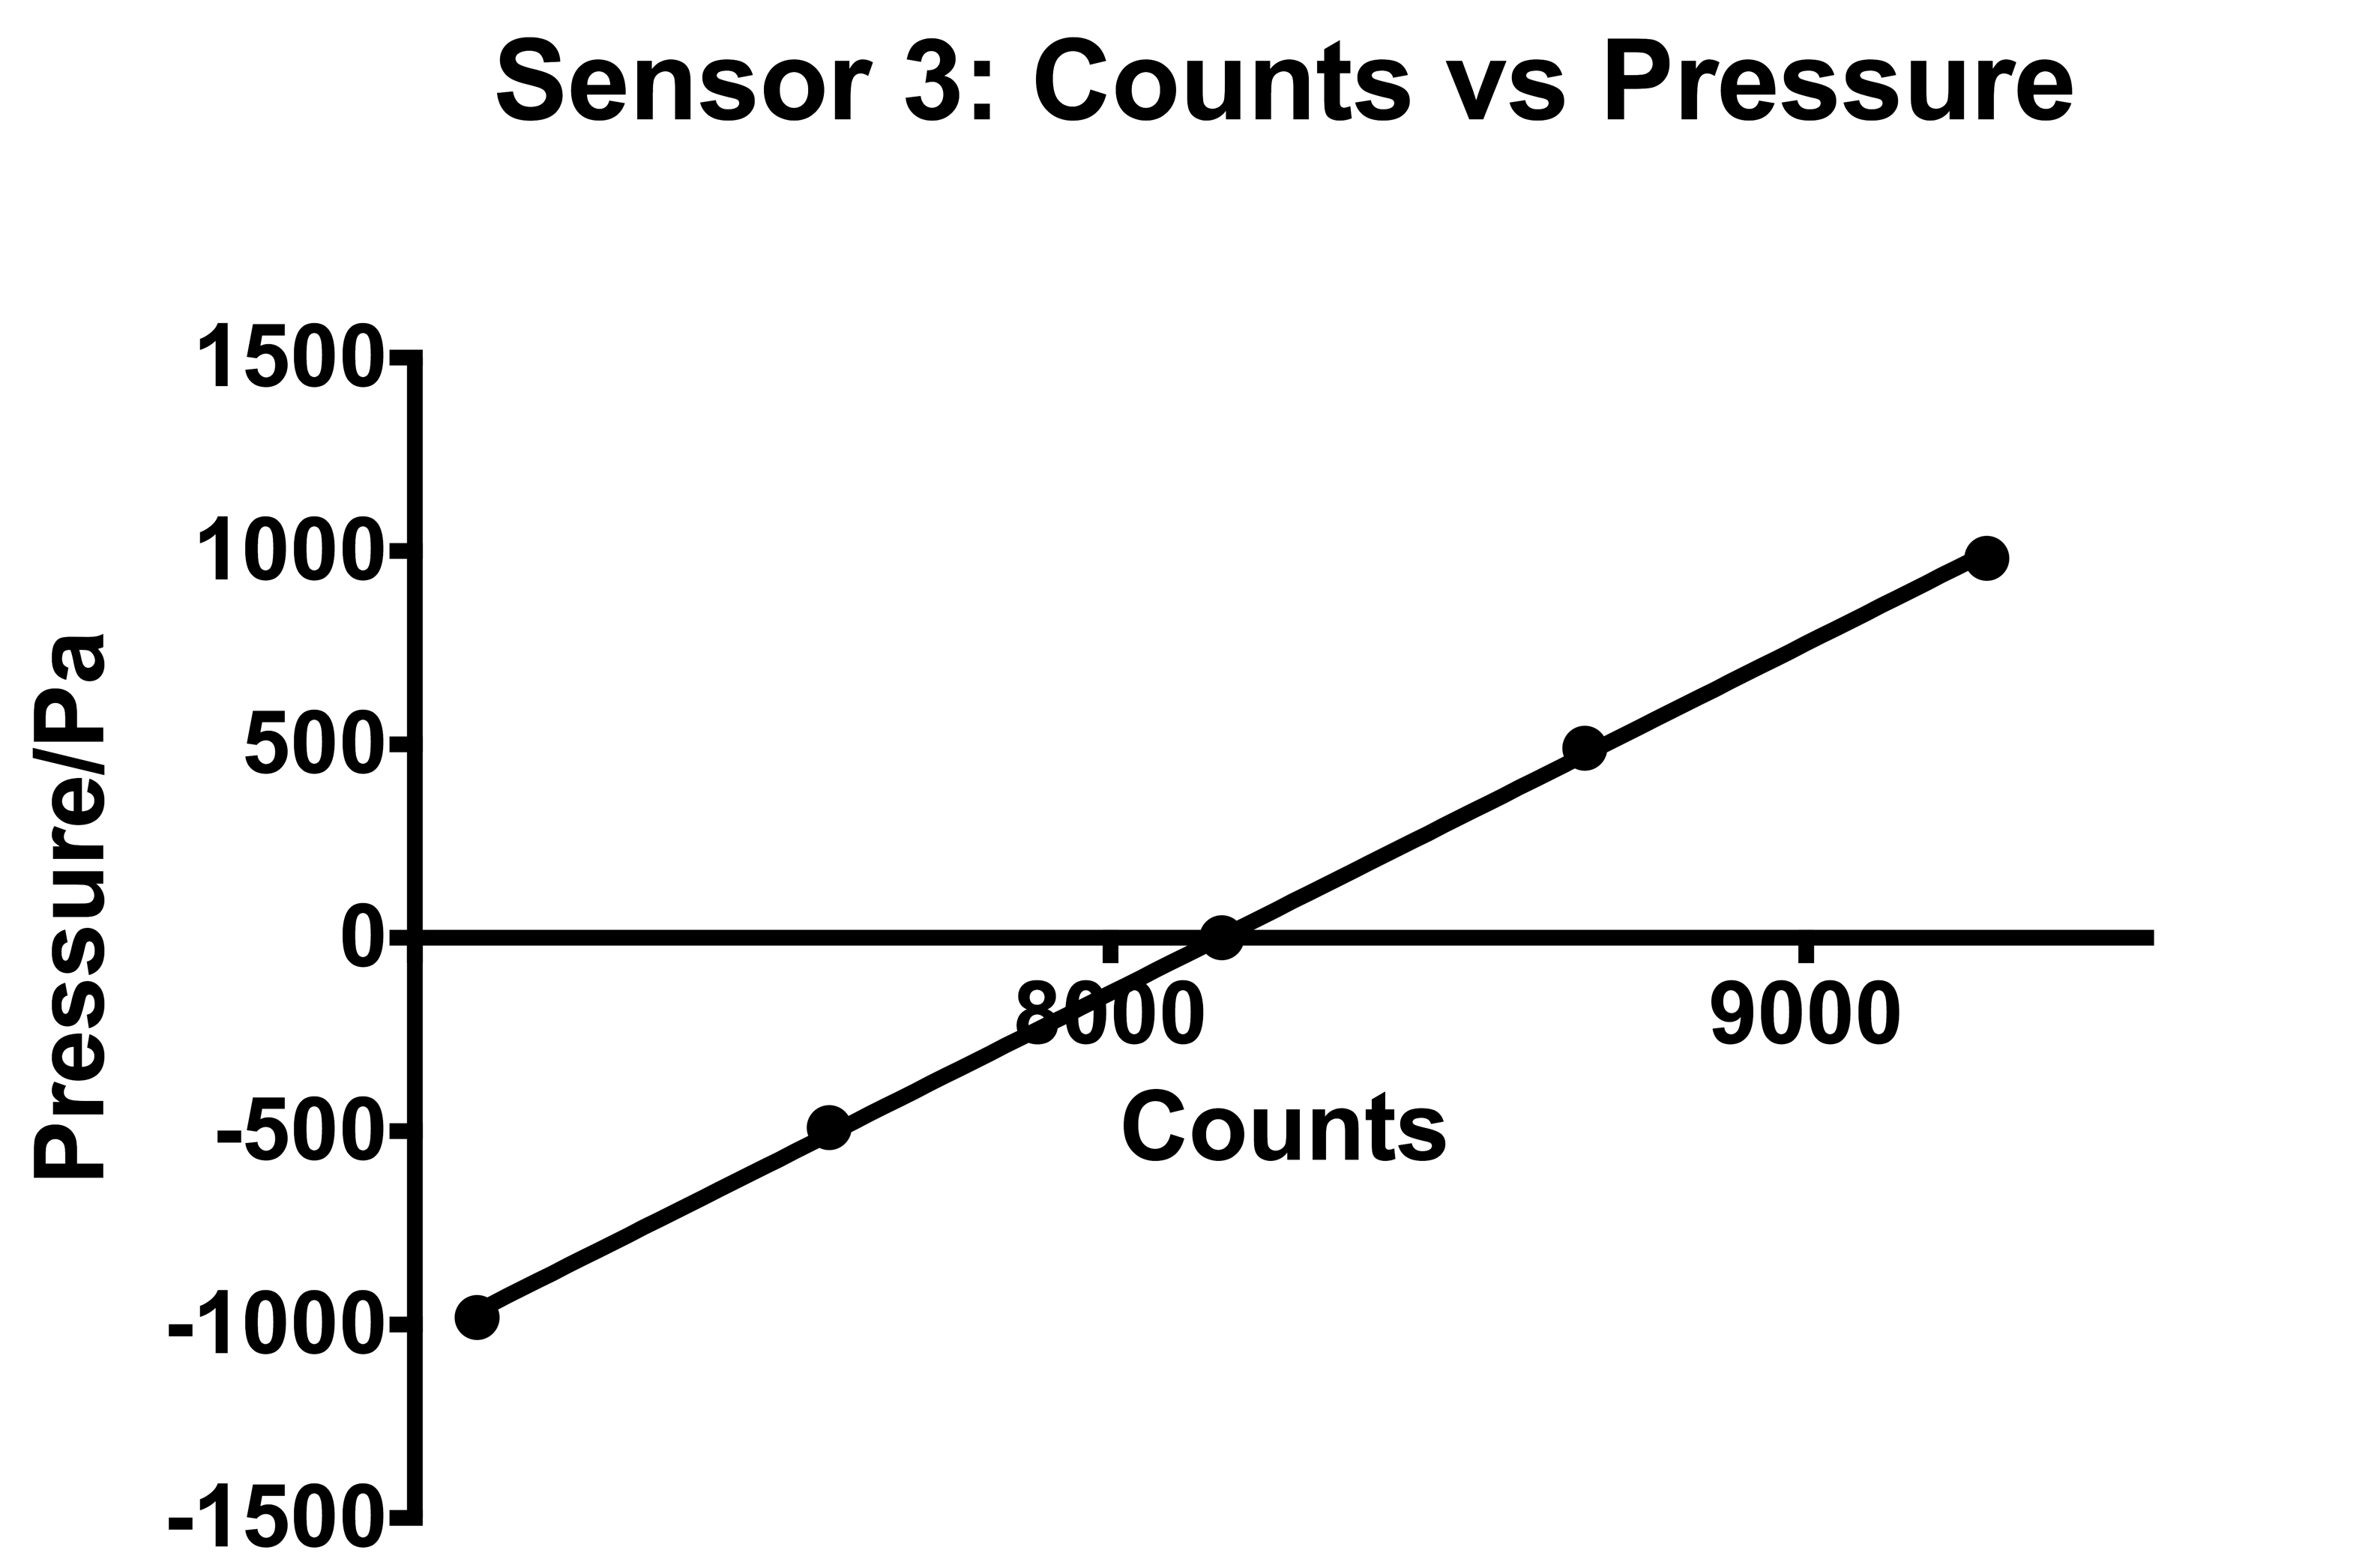
\includegraphics{s3.png}}}\hspace{5pt}
\subfloat{%
\resizebox*{8cm}{!}{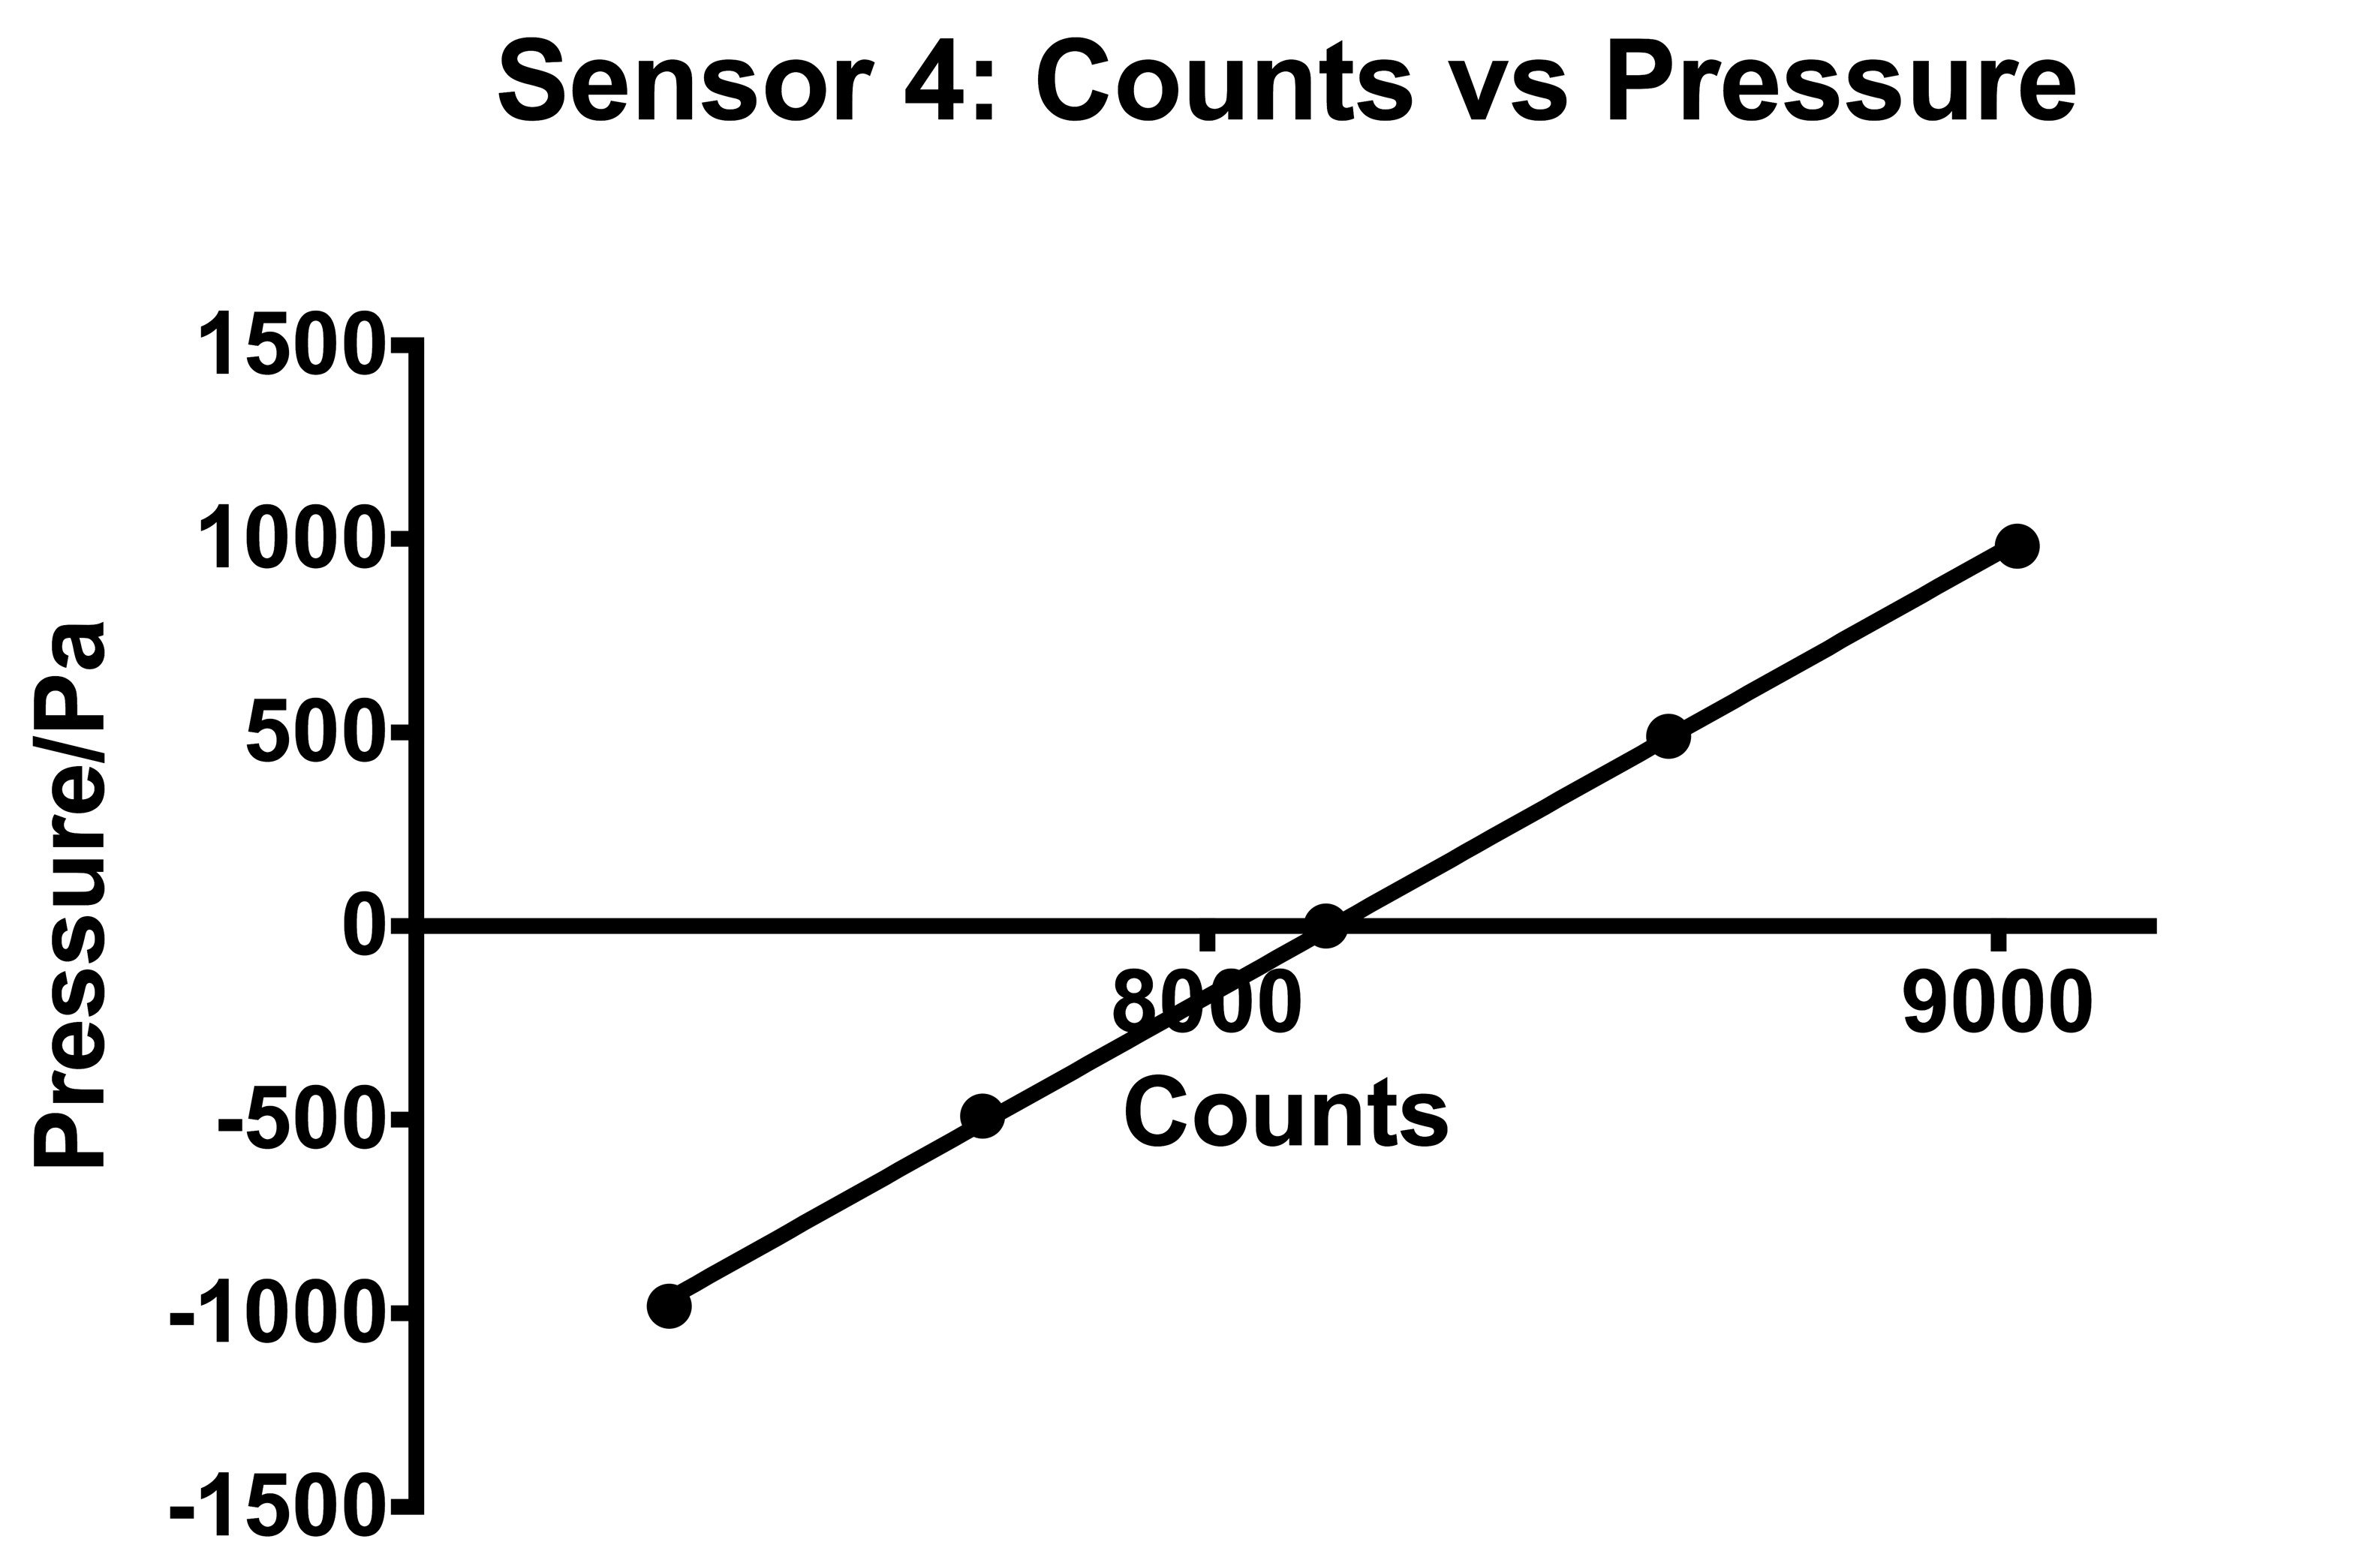
\includegraphics{s4.png}}}\hspace{5pt}
\caption{Graphs showing the relation between the decimal counts as output by the sensors and pressure on the ports in pascals exerted by a water column.} \label{fig:budgets1}
\end{figure}
\newpage
\section{Data filtering}
\thispagestyle{fancy}
The aim of this section is to filter the data that comes from the pressure sensor so that the noise of values fed into the controller is minimised. The speed of sampling also needs to be considered especially since four pressure sensors are sharing a single I2C line. There are many choices for data filters. 

A median filter takes a certain number of samples and outputs the median. This is useful when a sensor is known to output extreme values frequently. A common application of this filter is in ultrasonic range finders which work by sending out an ultrasonic pulse and receiving the reflection. The time between the pulse being sent and received is measured. The speed of sound at sea level is a constant. Thus, the distance can be calculated. Often, a sent pulse is not received and detected by the sensor which causes a timeout. In such an event, the sensor output can be extreme. A median filter however will completely disregard this value. In this project, the sensor is highly unlikely to output nonsensical values. Therefore, the use of median filter is not appropriate. 

A simple average filter on the other hand may be much more useful. The operation is quite simple. A certain number of samples is taken and averaged. The intensity of noise is minimised by increasing the window (number of samples taken). 

According to the Nyquist-Shannon theorem\cite{shan}, "\textit{If a function x(t) only contains frequencies higher than B hertz, it is completely determined by a series of points 1/(2B) seconds apart}". In other words, the sampling frequency must be more than twice the SPO frequency. As mentioned earlier, SPOs occur at around 2Hz. Therefore, the sampling frequency must be at least more than 4Hz. 

The sample time was measured as a function of the window size and the results are plotted below. 
\begin{figure}[h]
\centering
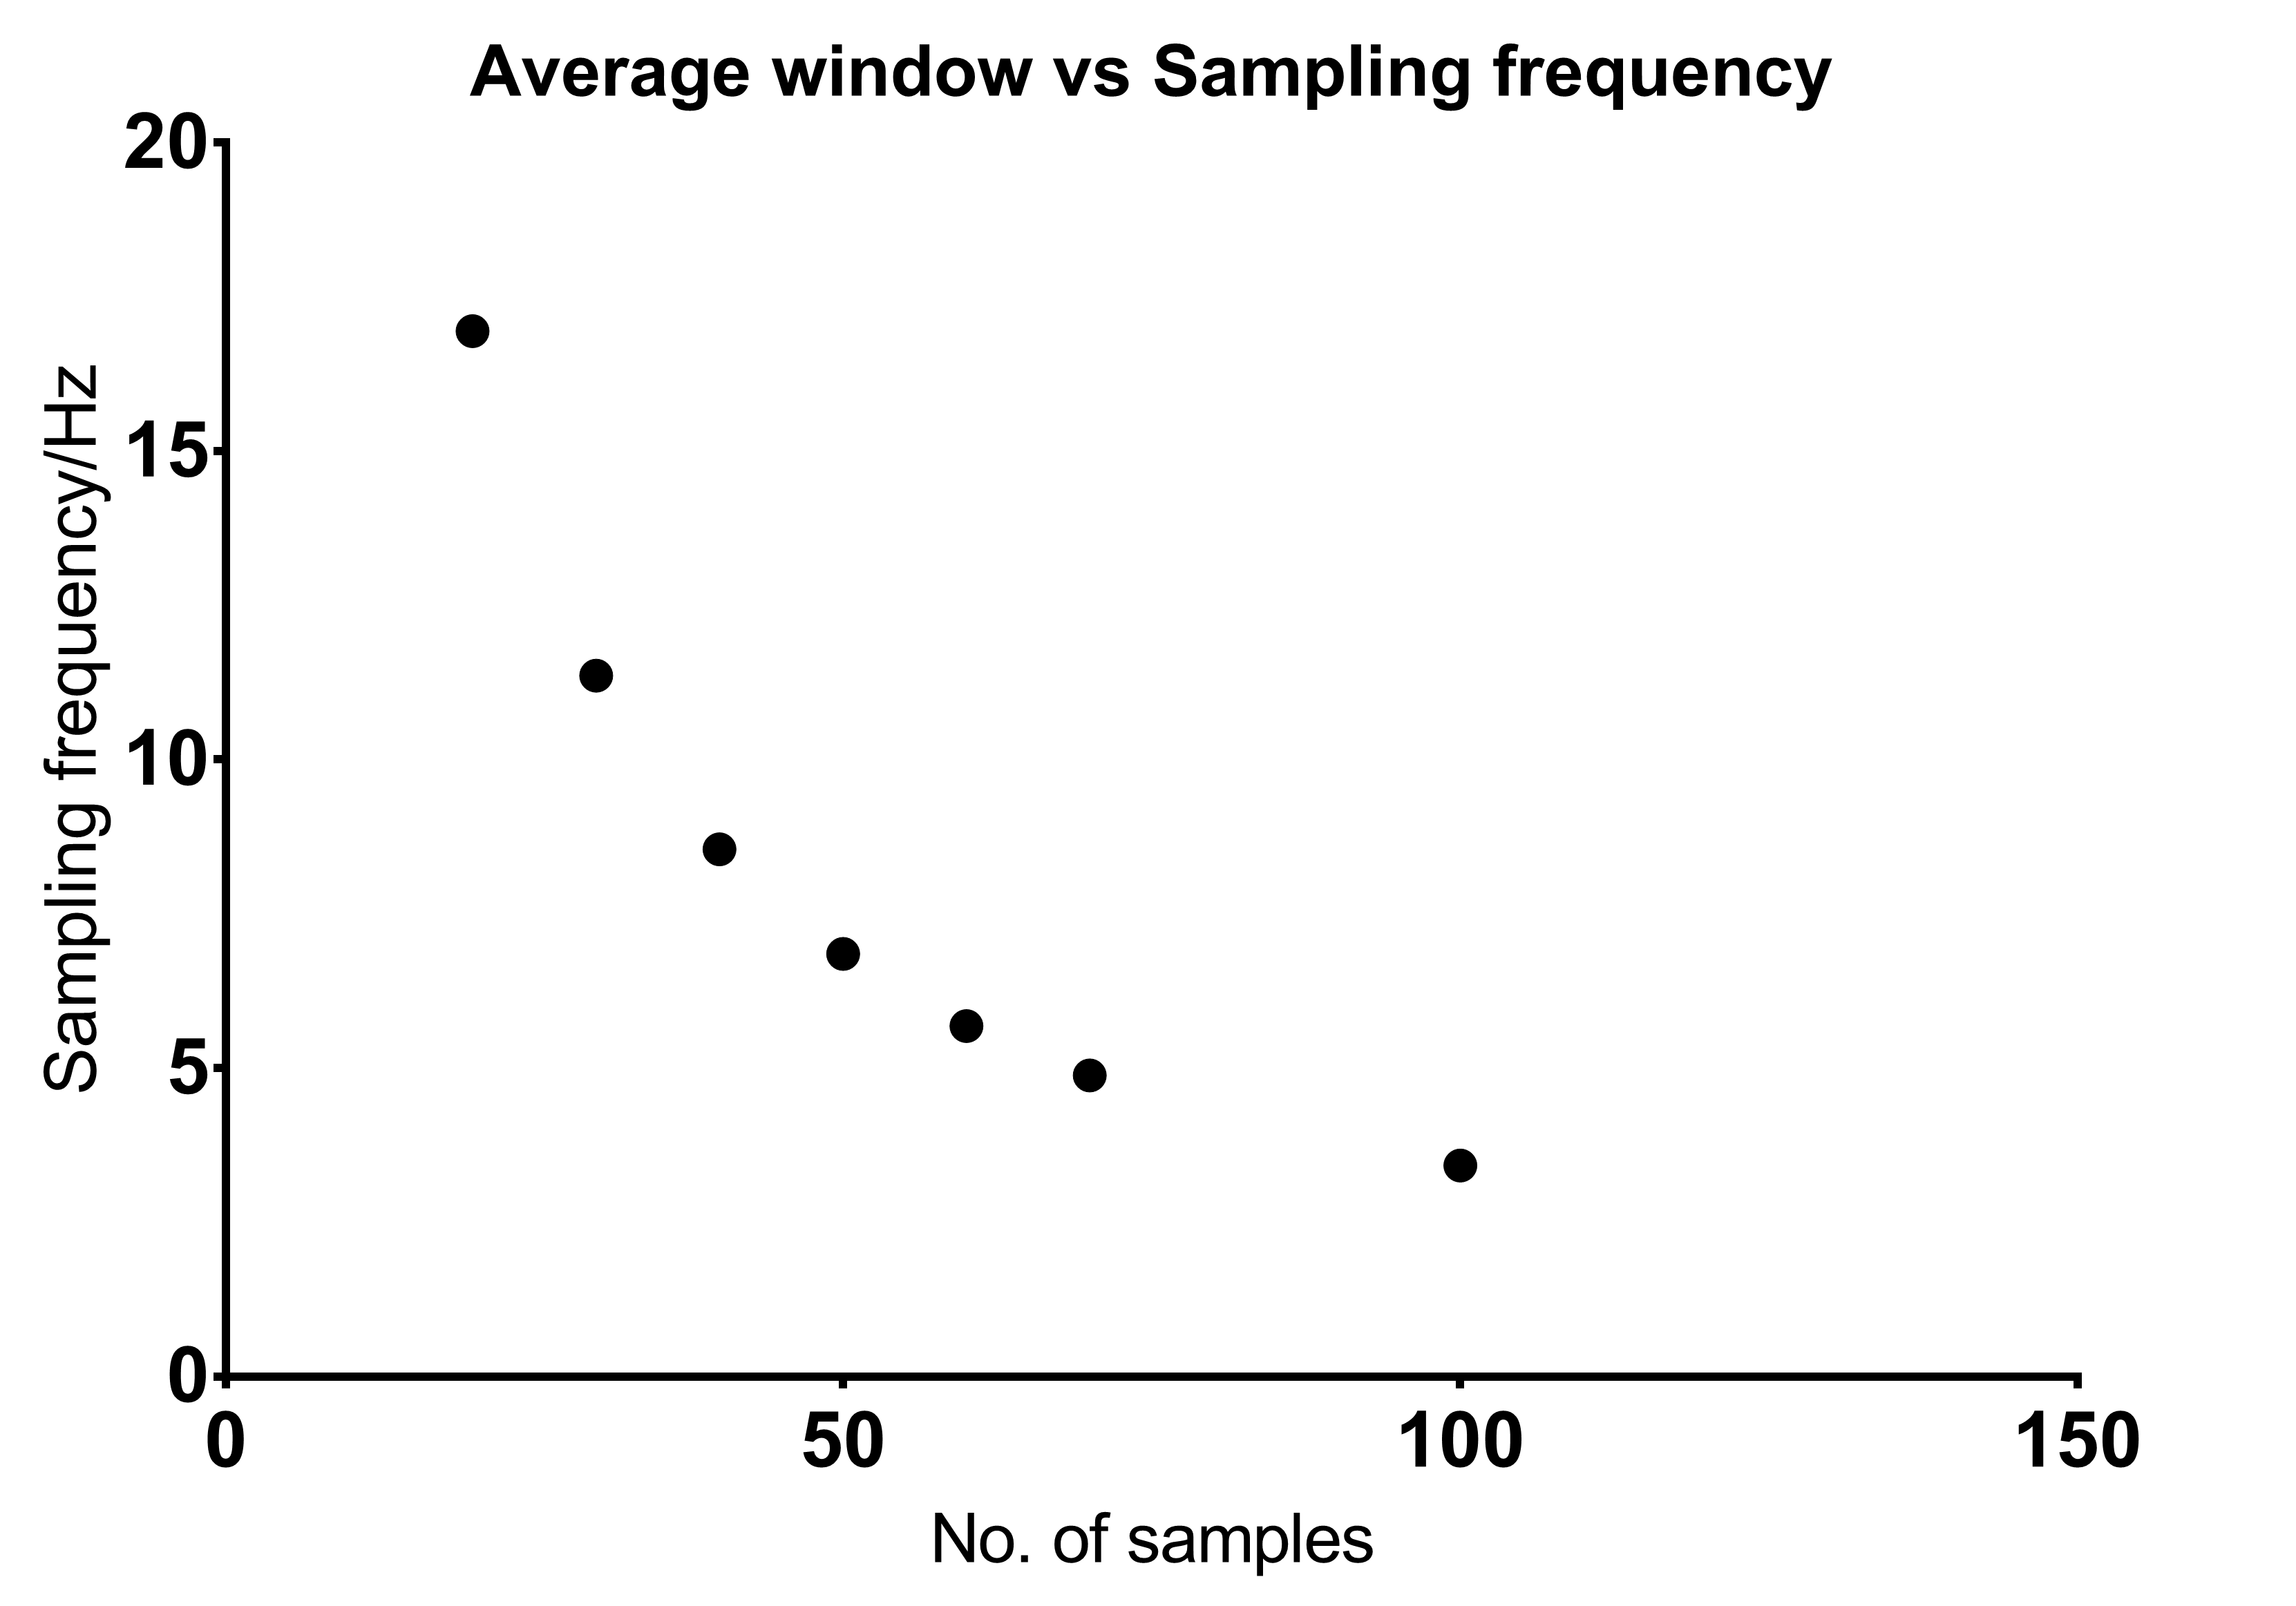
\includegraphics[scale=0.5]{samp.png}
\caption{Window size vs sampling frequency. An inversely proportional relation is apparent.}
\centering
\end{figure}

It seems that the sampling frequency is inversely proportional to the number of samples. This was confirmed by taking the log of both the frequency and the number of samples. 

\begin{equation}
N\propto\frac{1}{f}
\end{equation}
\begin{equation}
N=\frac{k}{f}
\end{equation}
\begin{equation}
\log(N)=\log(\frac{k}{f})
\end{equation}
\begin{equation}
\log(N)=\log(k)-\log(f)
\end{equation}
\newline
Plotting log(N) against log(f) gave the following result which proved the inversely proportional relation.
\begin{figure}[h]
\centering
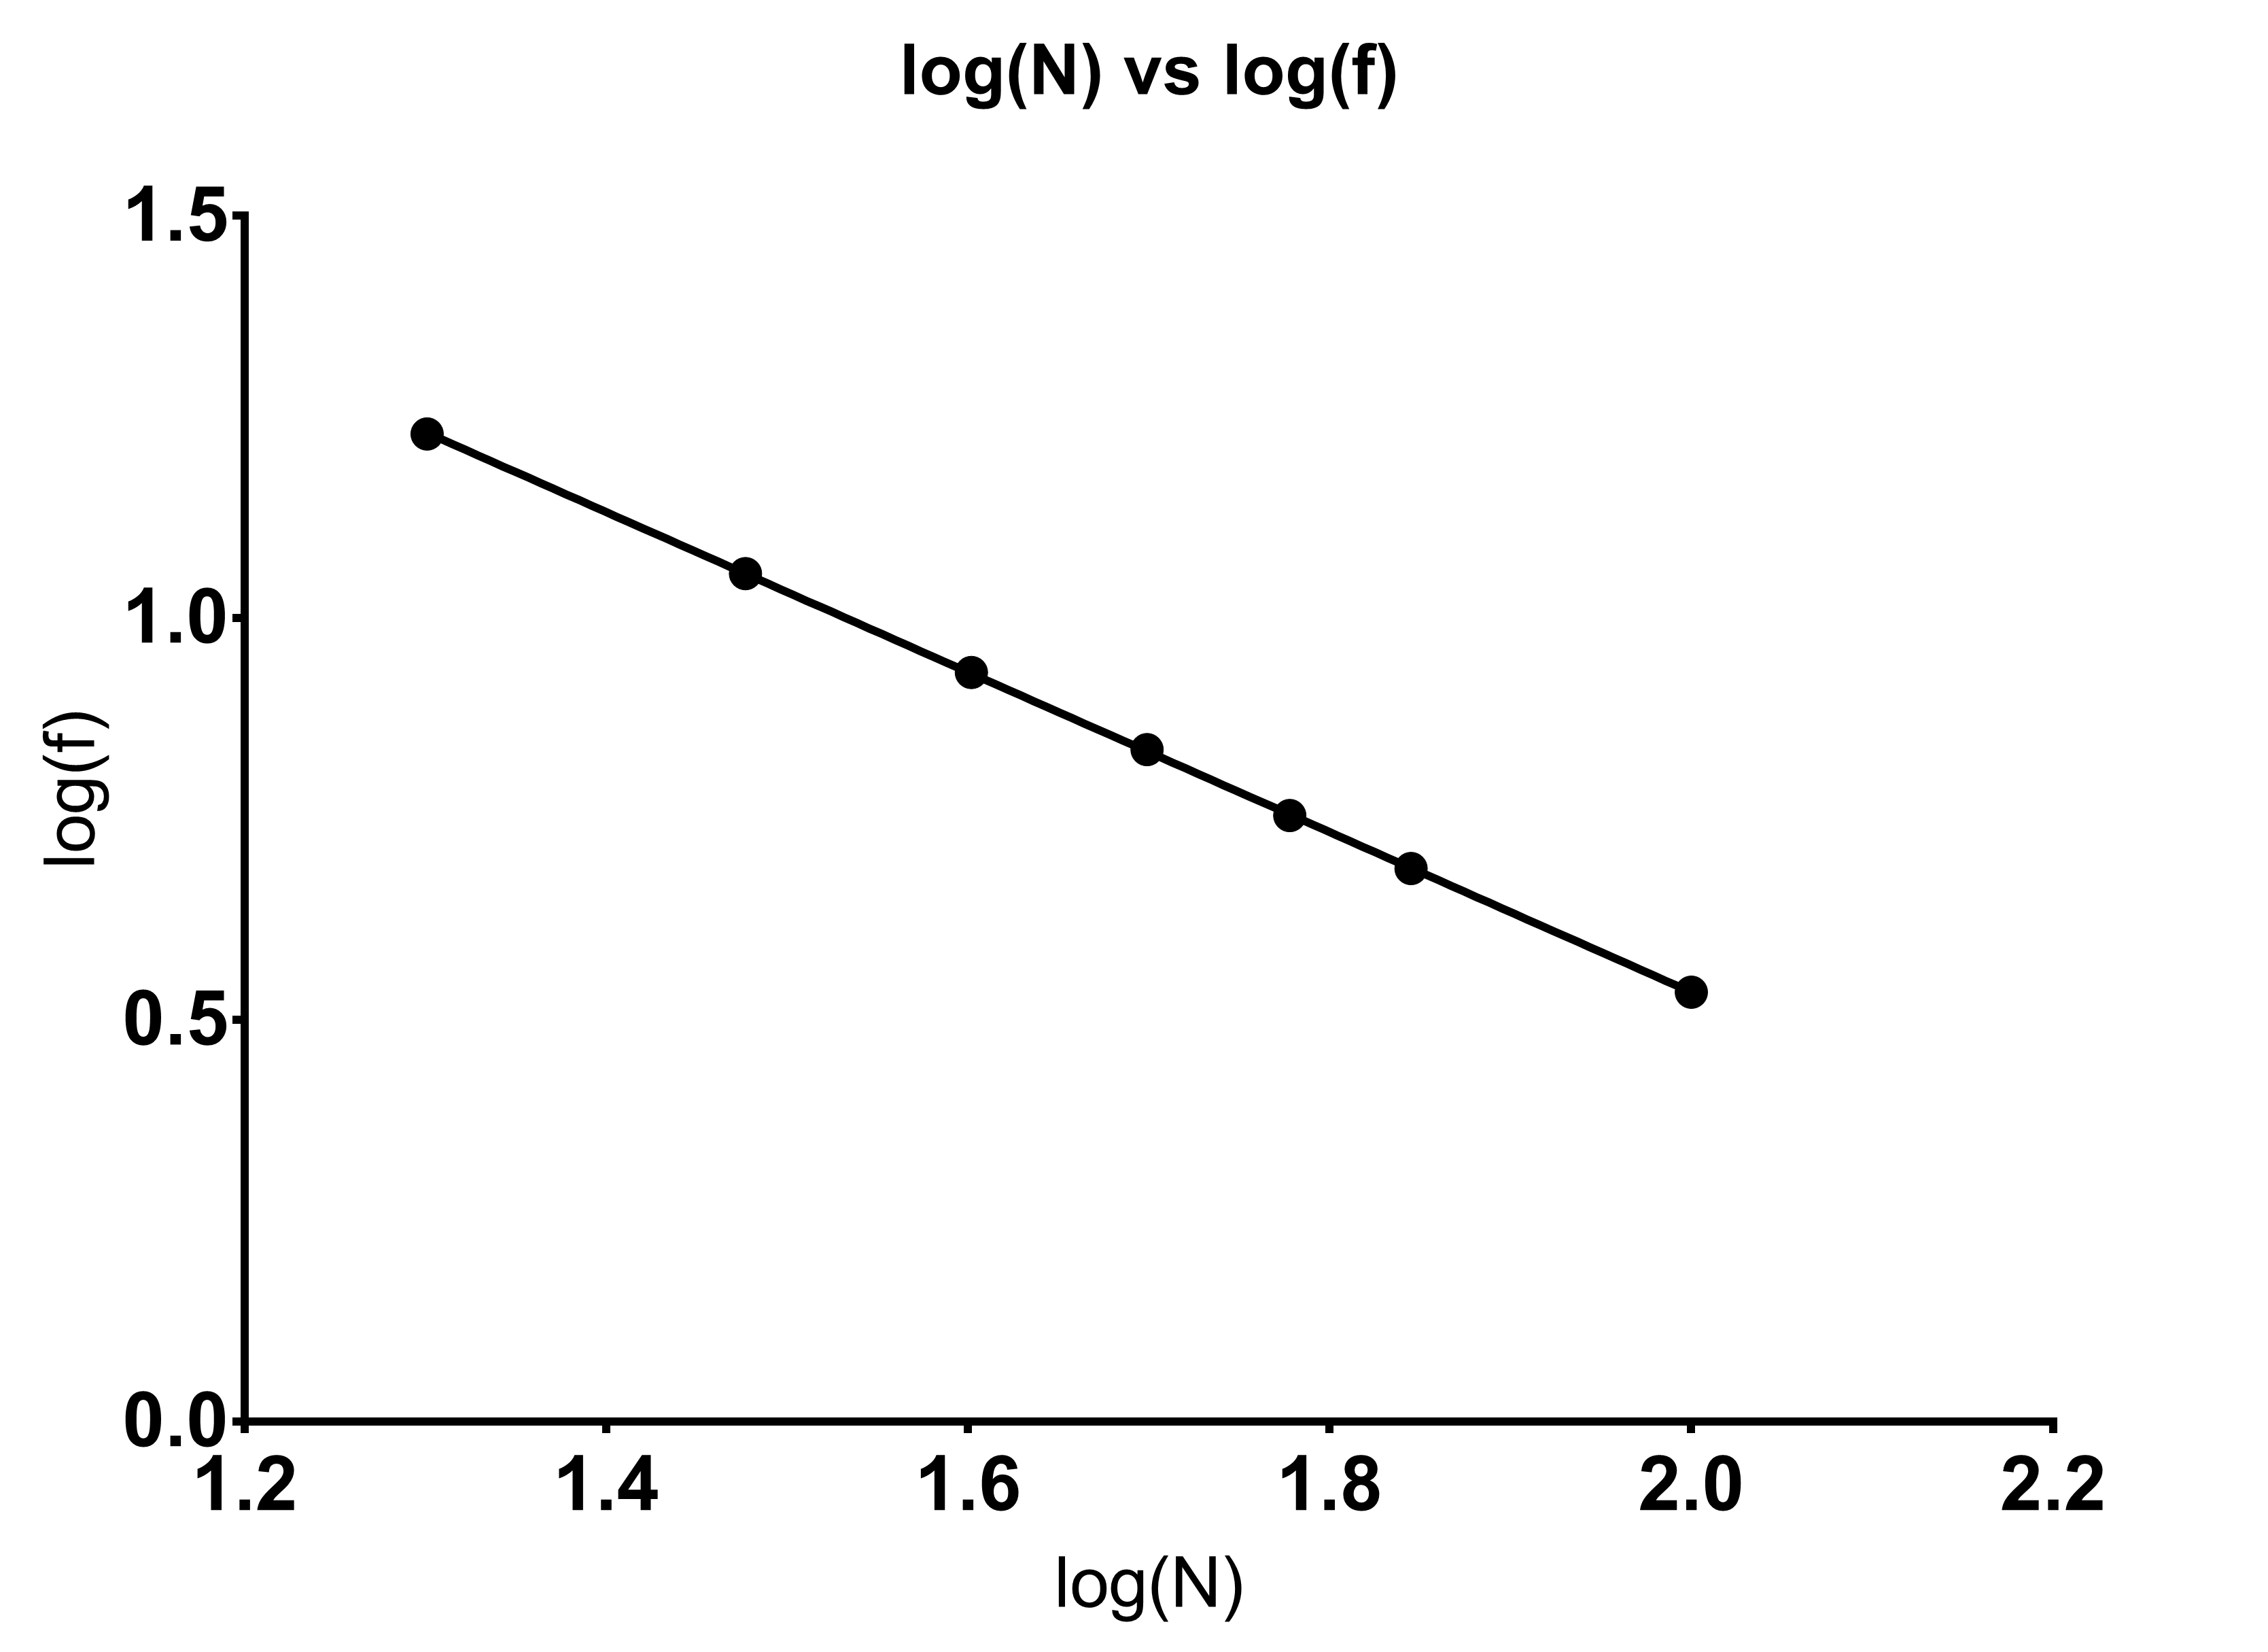
\includegraphics[scale=0.5]{log.png}
\caption{Log of N vs log of frequency. The linearity proves the inversely proportional relation. Also note that y-intercept is log of k.}
\centering
\end{figure}
\thispagestyle{fancy}
The graphing software calculated the y-intercept to be 2.525. This is also equal to log(k). Therefore k can be calculated to be $10^{2.525}$ which is 334.97. 

Now the window size at f=4Hz can be calculated. To comply with the Nyquist-Shannon theorem, the maximum window size can be 84. There needs to be a large margin to keep the system responsive which is essential to suppress a fast oscillation. Window size of 50 was chosen to ensure the system can keep up with the oscillation. 
\chapter{Physical design}
This chapter will focus on the physical design of the wing that will be placed in the wind tunnel. The mechanism to create gusts in the wind tunnel will also be outlined. 
\section{Design of Main Wing}
\thispagestyle{fancy}
To calculate the lift produced by the wing, local static pressure readings from several points along the top and the bottom of the wing are required. The easiest way to do this is by creating pressure tappings at specified points along the wing surface.
\newline
\newline
Firstly, the NACA2412 aerofoil was chosen for the wing. This decision was not entirely arbitrary. The moderate thickness of $12\%$ chord length and a camber of $2 \%$ at $40\%$ chord length. This increases the L/D ratio and is good for low speed flight which is the regime most UAVs fly in.  
\newline
\newline
The wing has a chord of 0.25m and a span of 0.35m. The trailing edge flap begins at x/c of 0.75. The pressure tappings are at x/c of 0.2, 0.4 and 0.6. There are probably better locations for these pressure tappings which will yield better lift estimates. However, finding the optimum locations is a large task and can be a separate project. For my project, the accuracy of the lift estimate is not highly important. The aim is to produce a controller that responds well to a change in airflow. Therefore, a lift estimator that can give values within 10$\%$ of the actual lift on average will be acceptable to test the response of the control system. The lift estimator is described in chapter 6. 
\begin{figure}[H]
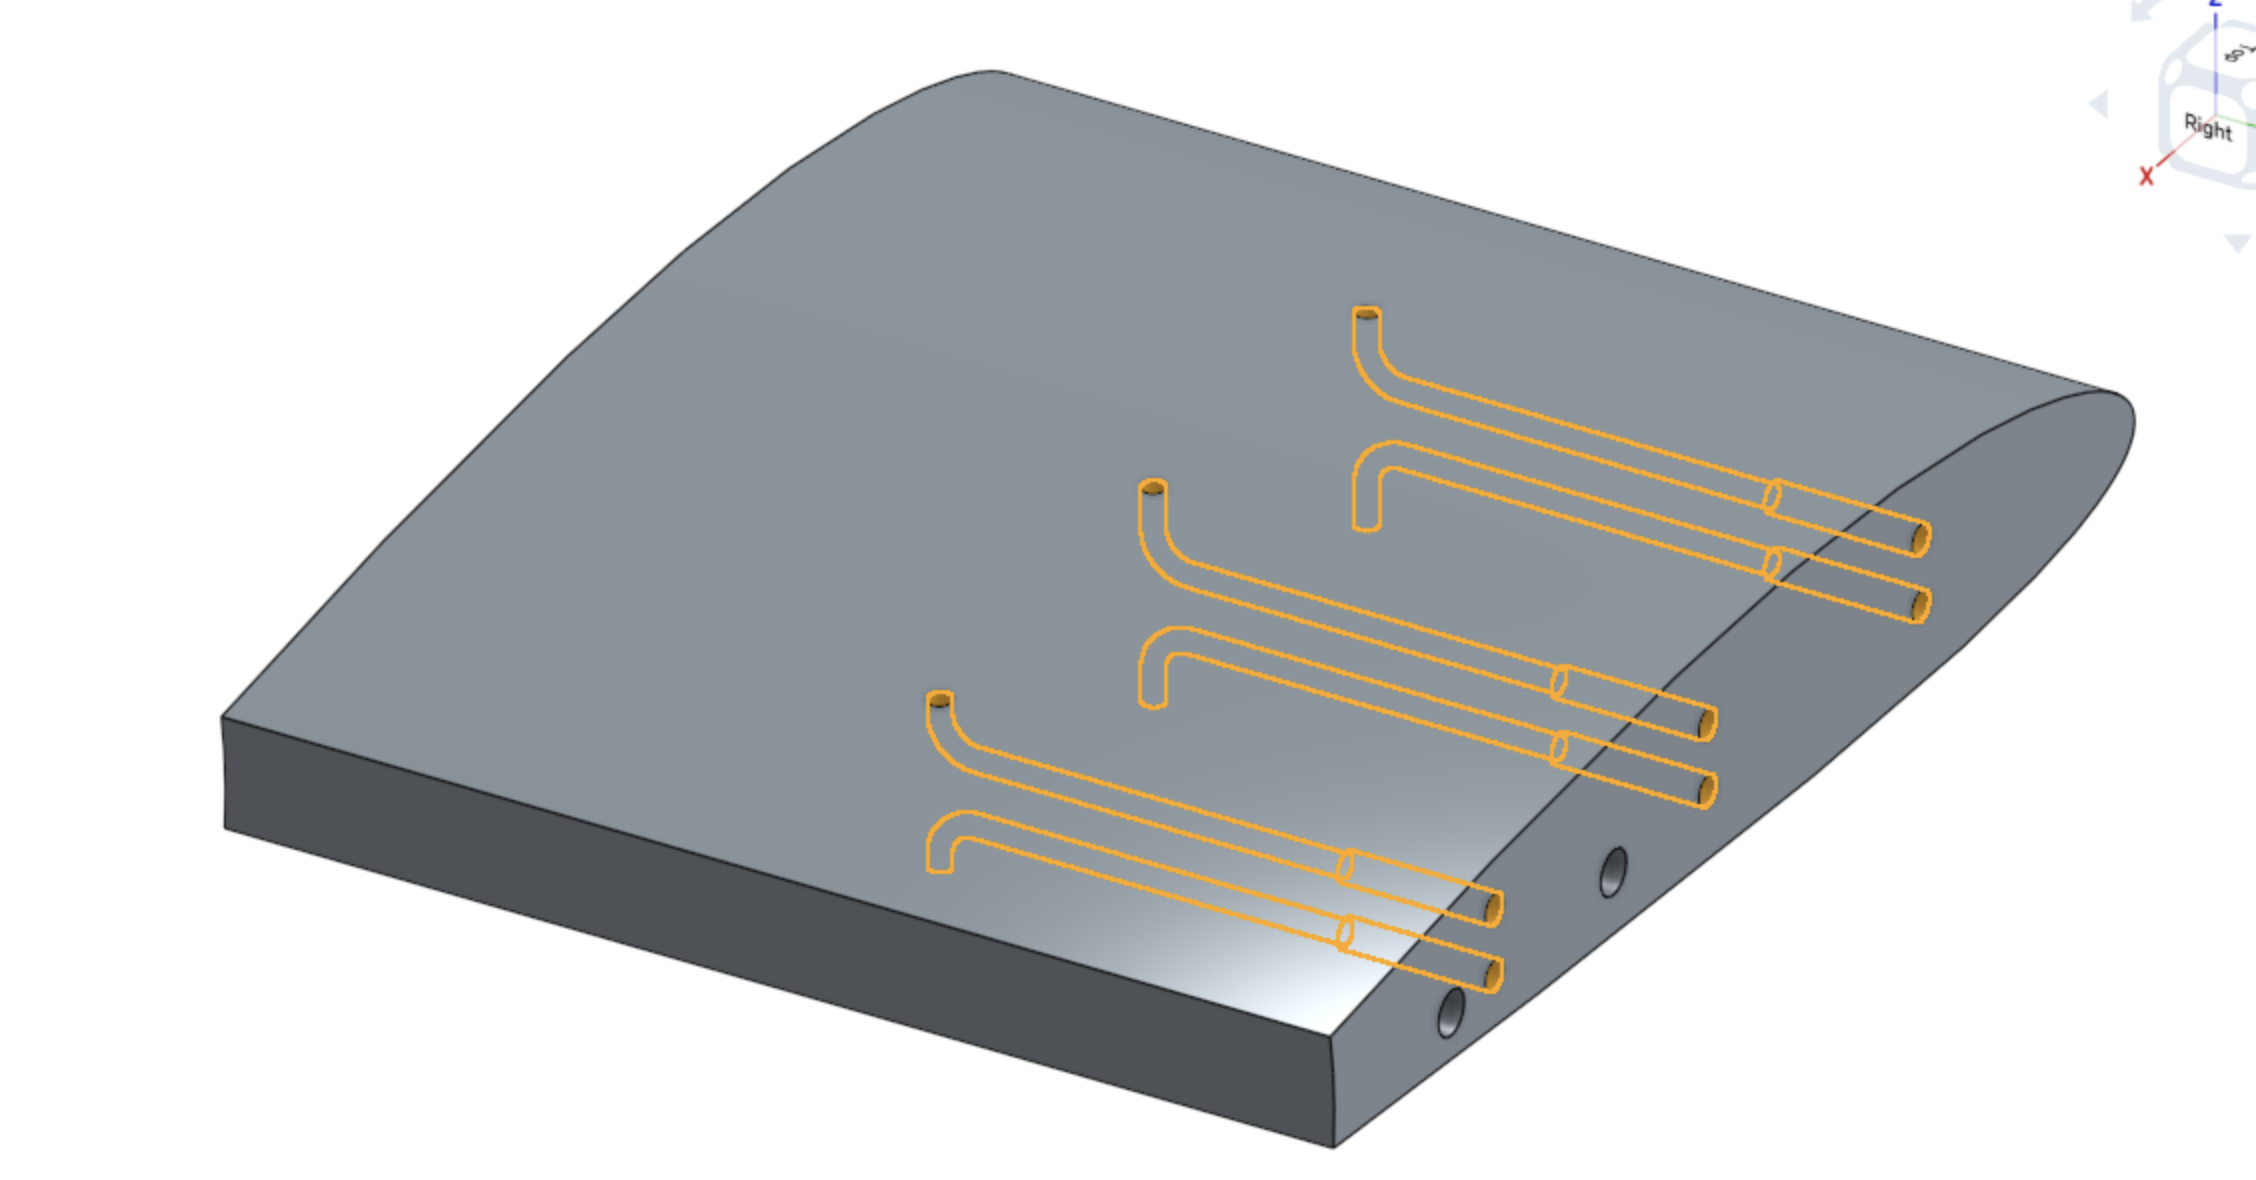
\includegraphics[width=0.7\textwidth,center]{wingmid.png}
\caption{Midsection of the wing with the internal tubing highlighted. The trailing edge flap is not included.}
\end{figure}
\newpage
\section{Gust Generator}
\thispagestyle{fancy}

To simulate an impulsive change in airspeed, a "gust generator" will be placed upstream from the wing. This consists of two NACA0015 airfoils with chord of 0.25 m and 0.5m span coupled to servos. The diagram below illustrates the configuration.

As the flaps move closer together, the airspeed of the flow between them will increase because of the decreasing cross-sectional area. This is simply due to conservation of mass. 
\begin{equation}
\dot{m} = \rho V A
\end{equation}
\begin{figure}[H]
\centering
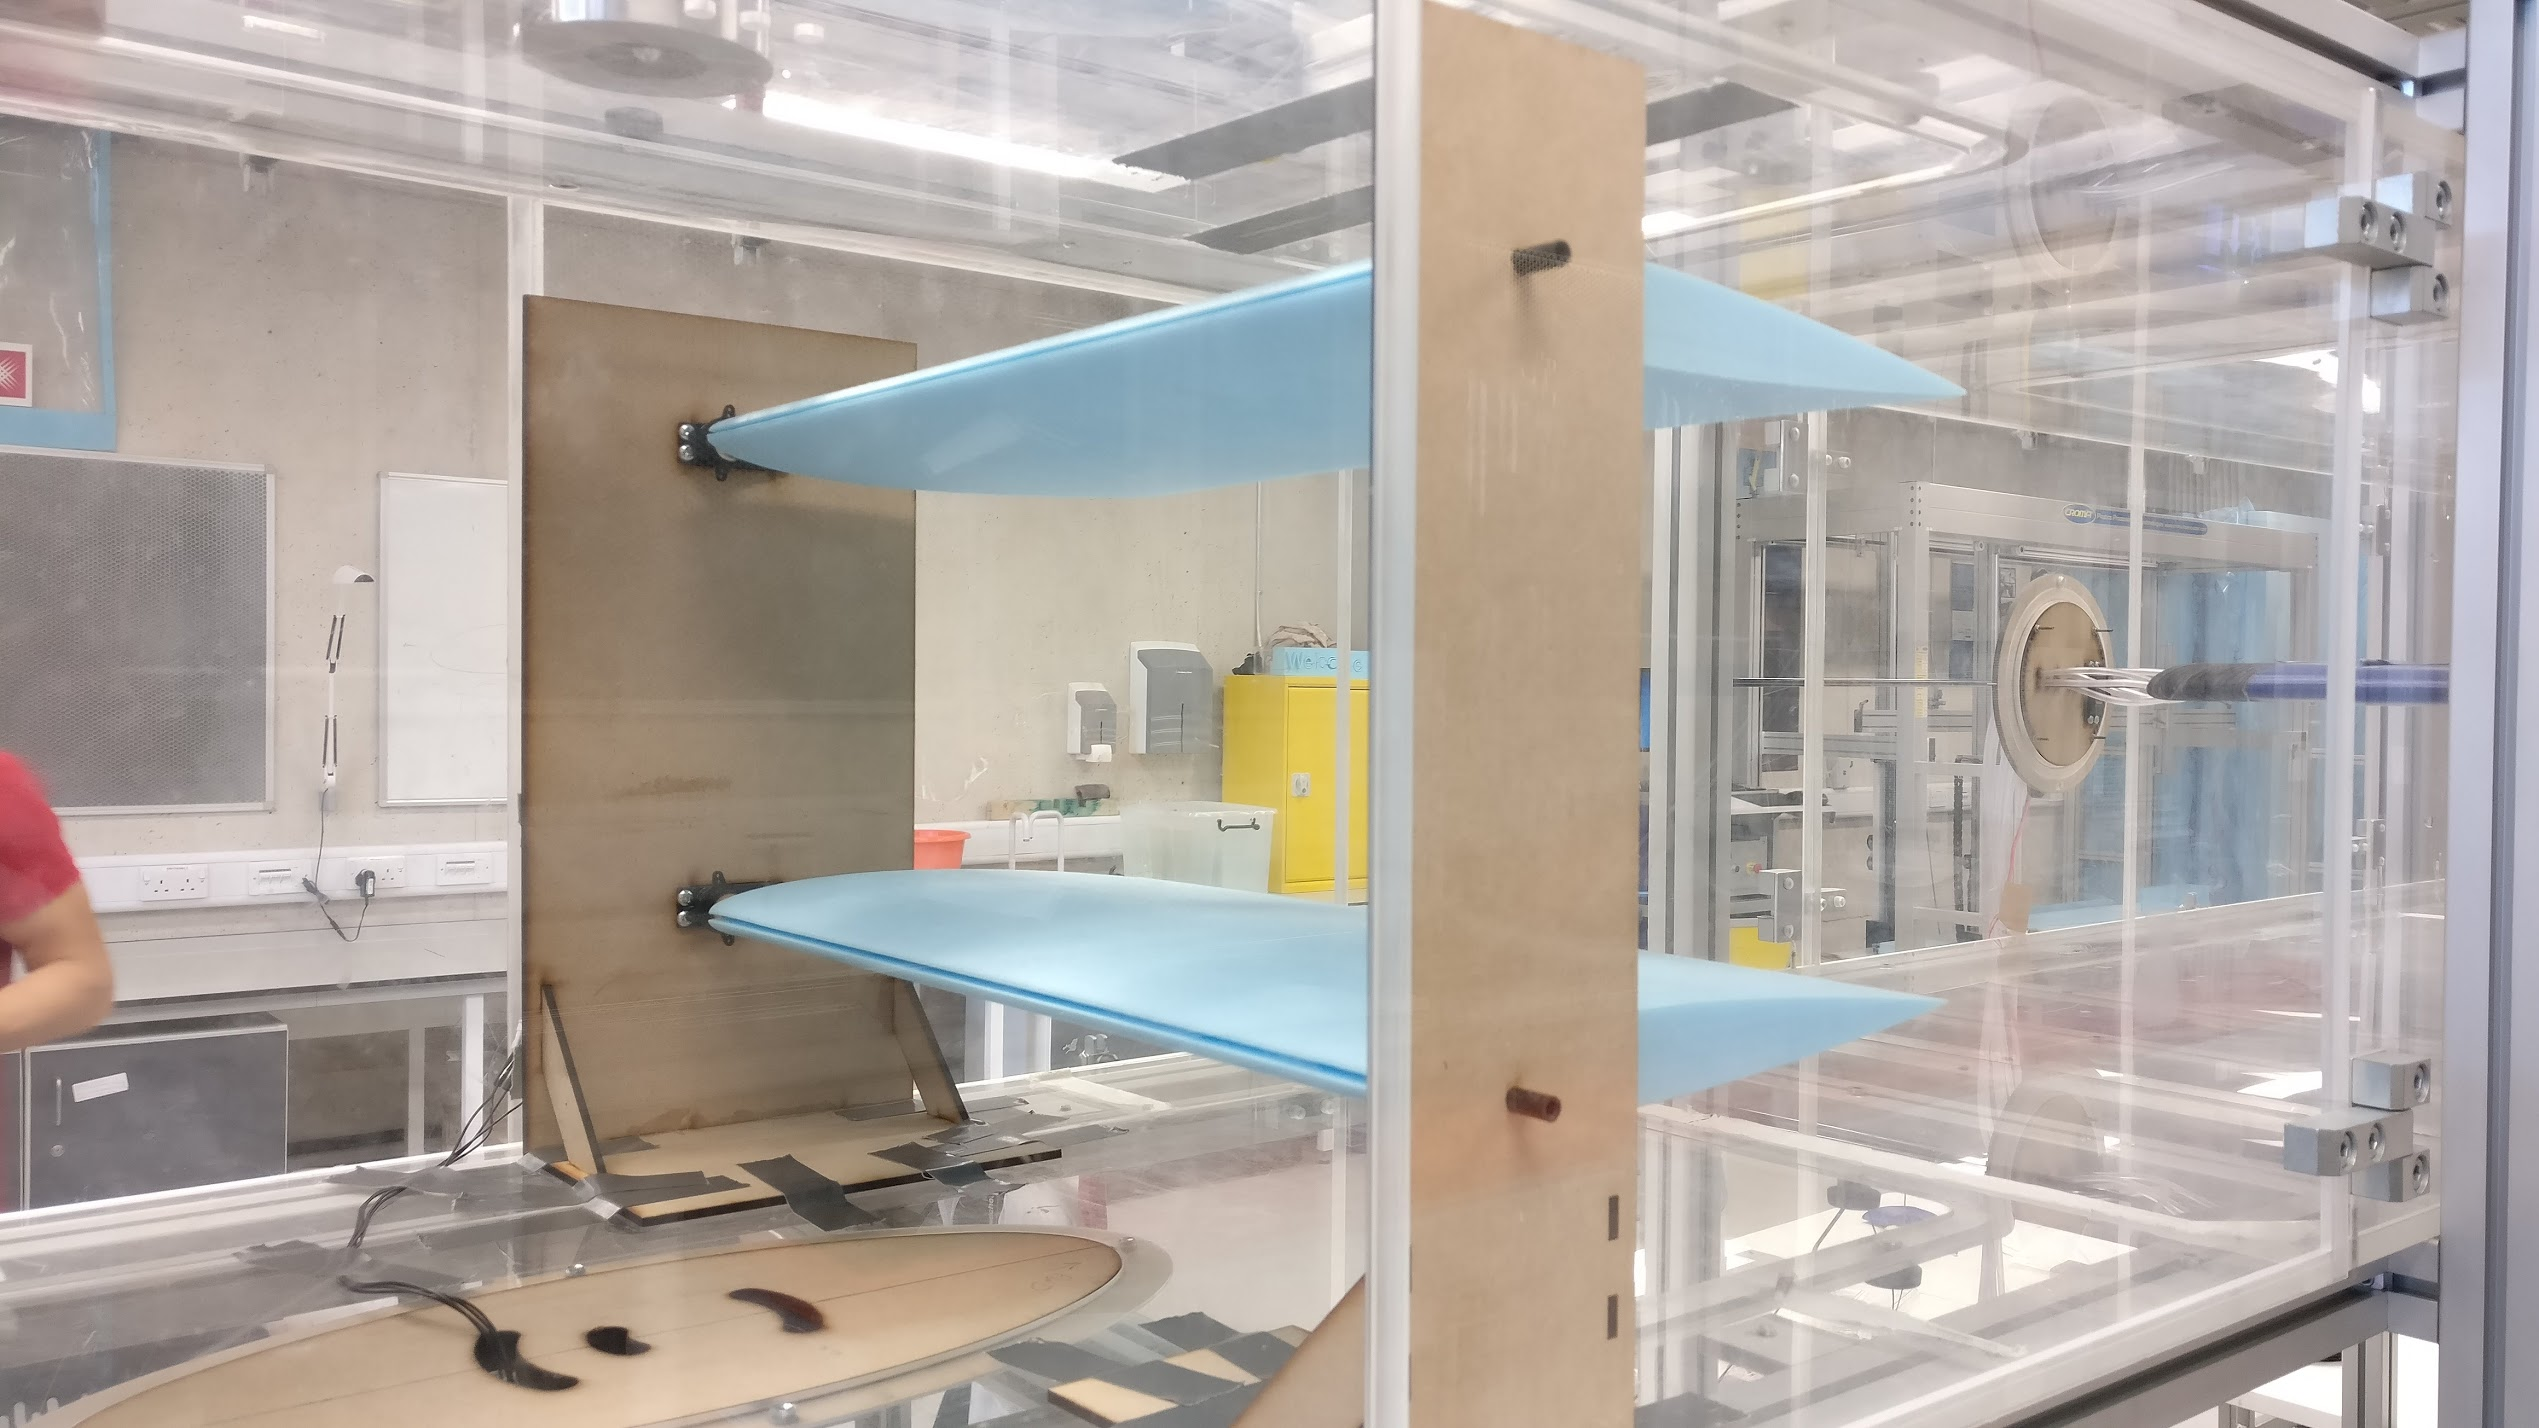
\includegraphics[scale=0.1]{gust.jpg}
\caption{Gust generator in the wind tunnel}
\centering
\end{figure}
A detailed description of the entire setup and manufacturing processes used can be found in Appendix A.
\newpage
\thispagestyle{fancy}
\chapter{Plant dynamics and Simulink modelling}
In this section, the dynamics of the plant will be estimated and analysed in MATLAB/Simulink to get initial estimates for the PID gains. There are two blocks in the plant for which a transfer function is needed. The first section will investigate how an input signal (PWM) translates to an angular displacement in the servo. Then, how the angle changes the $C_{L}$ and consequently the lift production will need to be understood. Firstly, an actuator needs to be chosen to move the flap. 
\section{Actuator}
\thispagestyle{fancy}
The SPO is a short lived and fast changing phenomenon. It is important to have a mechanism that does not create too much lag between the generation of the control signal and the actuation completing. A significant lag can even reinforce the oscillation and create dynamic instability. In this case the system response would have to be slowed down to stabilise the system. This will increase the settling time and would be a great compromise. A BMS-631 servo coupled to the trailing edge flap of the wing was used. The manufacturer states that it can turn 60$^{\circ}$ in 0.10 secs at 5V input voltage and 0.08 secs at 6V. This is
extremely fast compared to other servos on the market and is the most suitable device for this project. The manufacturer does not provide information on exactly how the angular displacement changes with time. The speed mentioned above is not sufficient information to give an accurate representation of the servo dynamics which many sources \cite{etkin} claim is a first order function. The performance of the servo will be measured so that a close approximation of the plant can be analysed before testing commences. 
\begin{figure}[H]
\centering
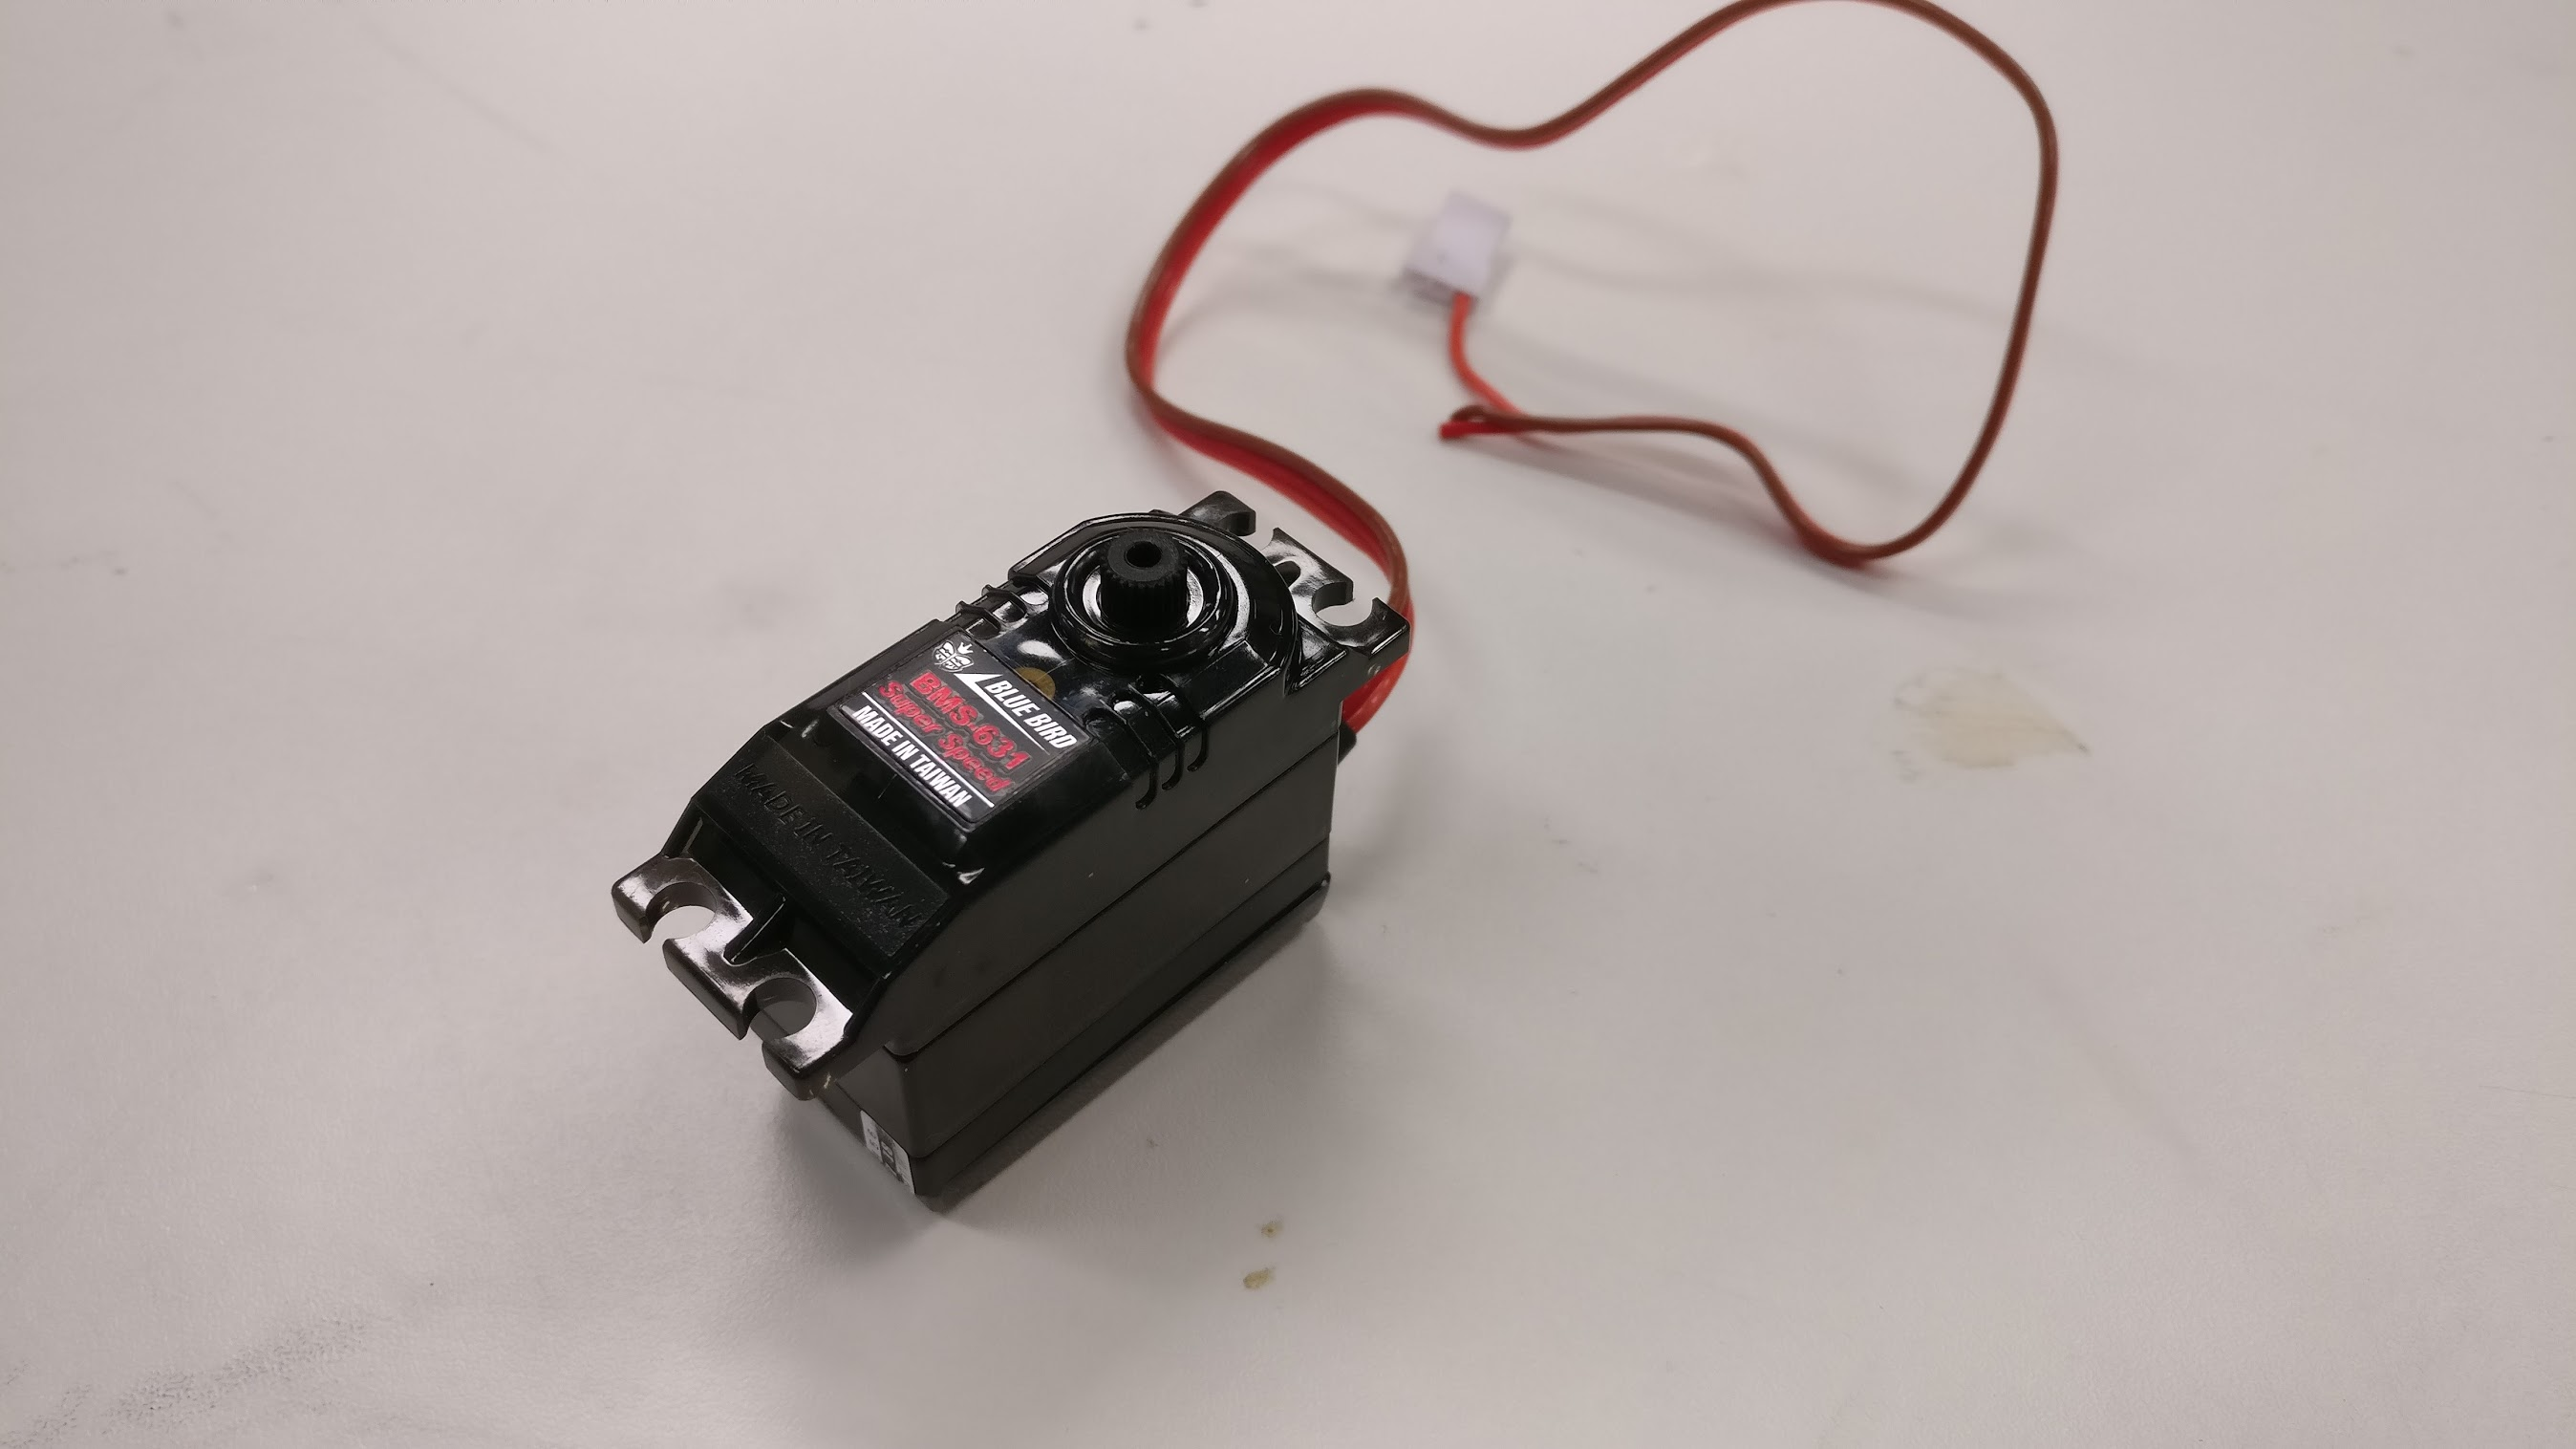
\includegraphics[scale=0.08]{servo.jpg}
\caption{The BMS-631 servo used to deflect the flap}
\centering
\end{figure}
\section{Dynamics of the servo}
\begin{figure}[h]
\centering
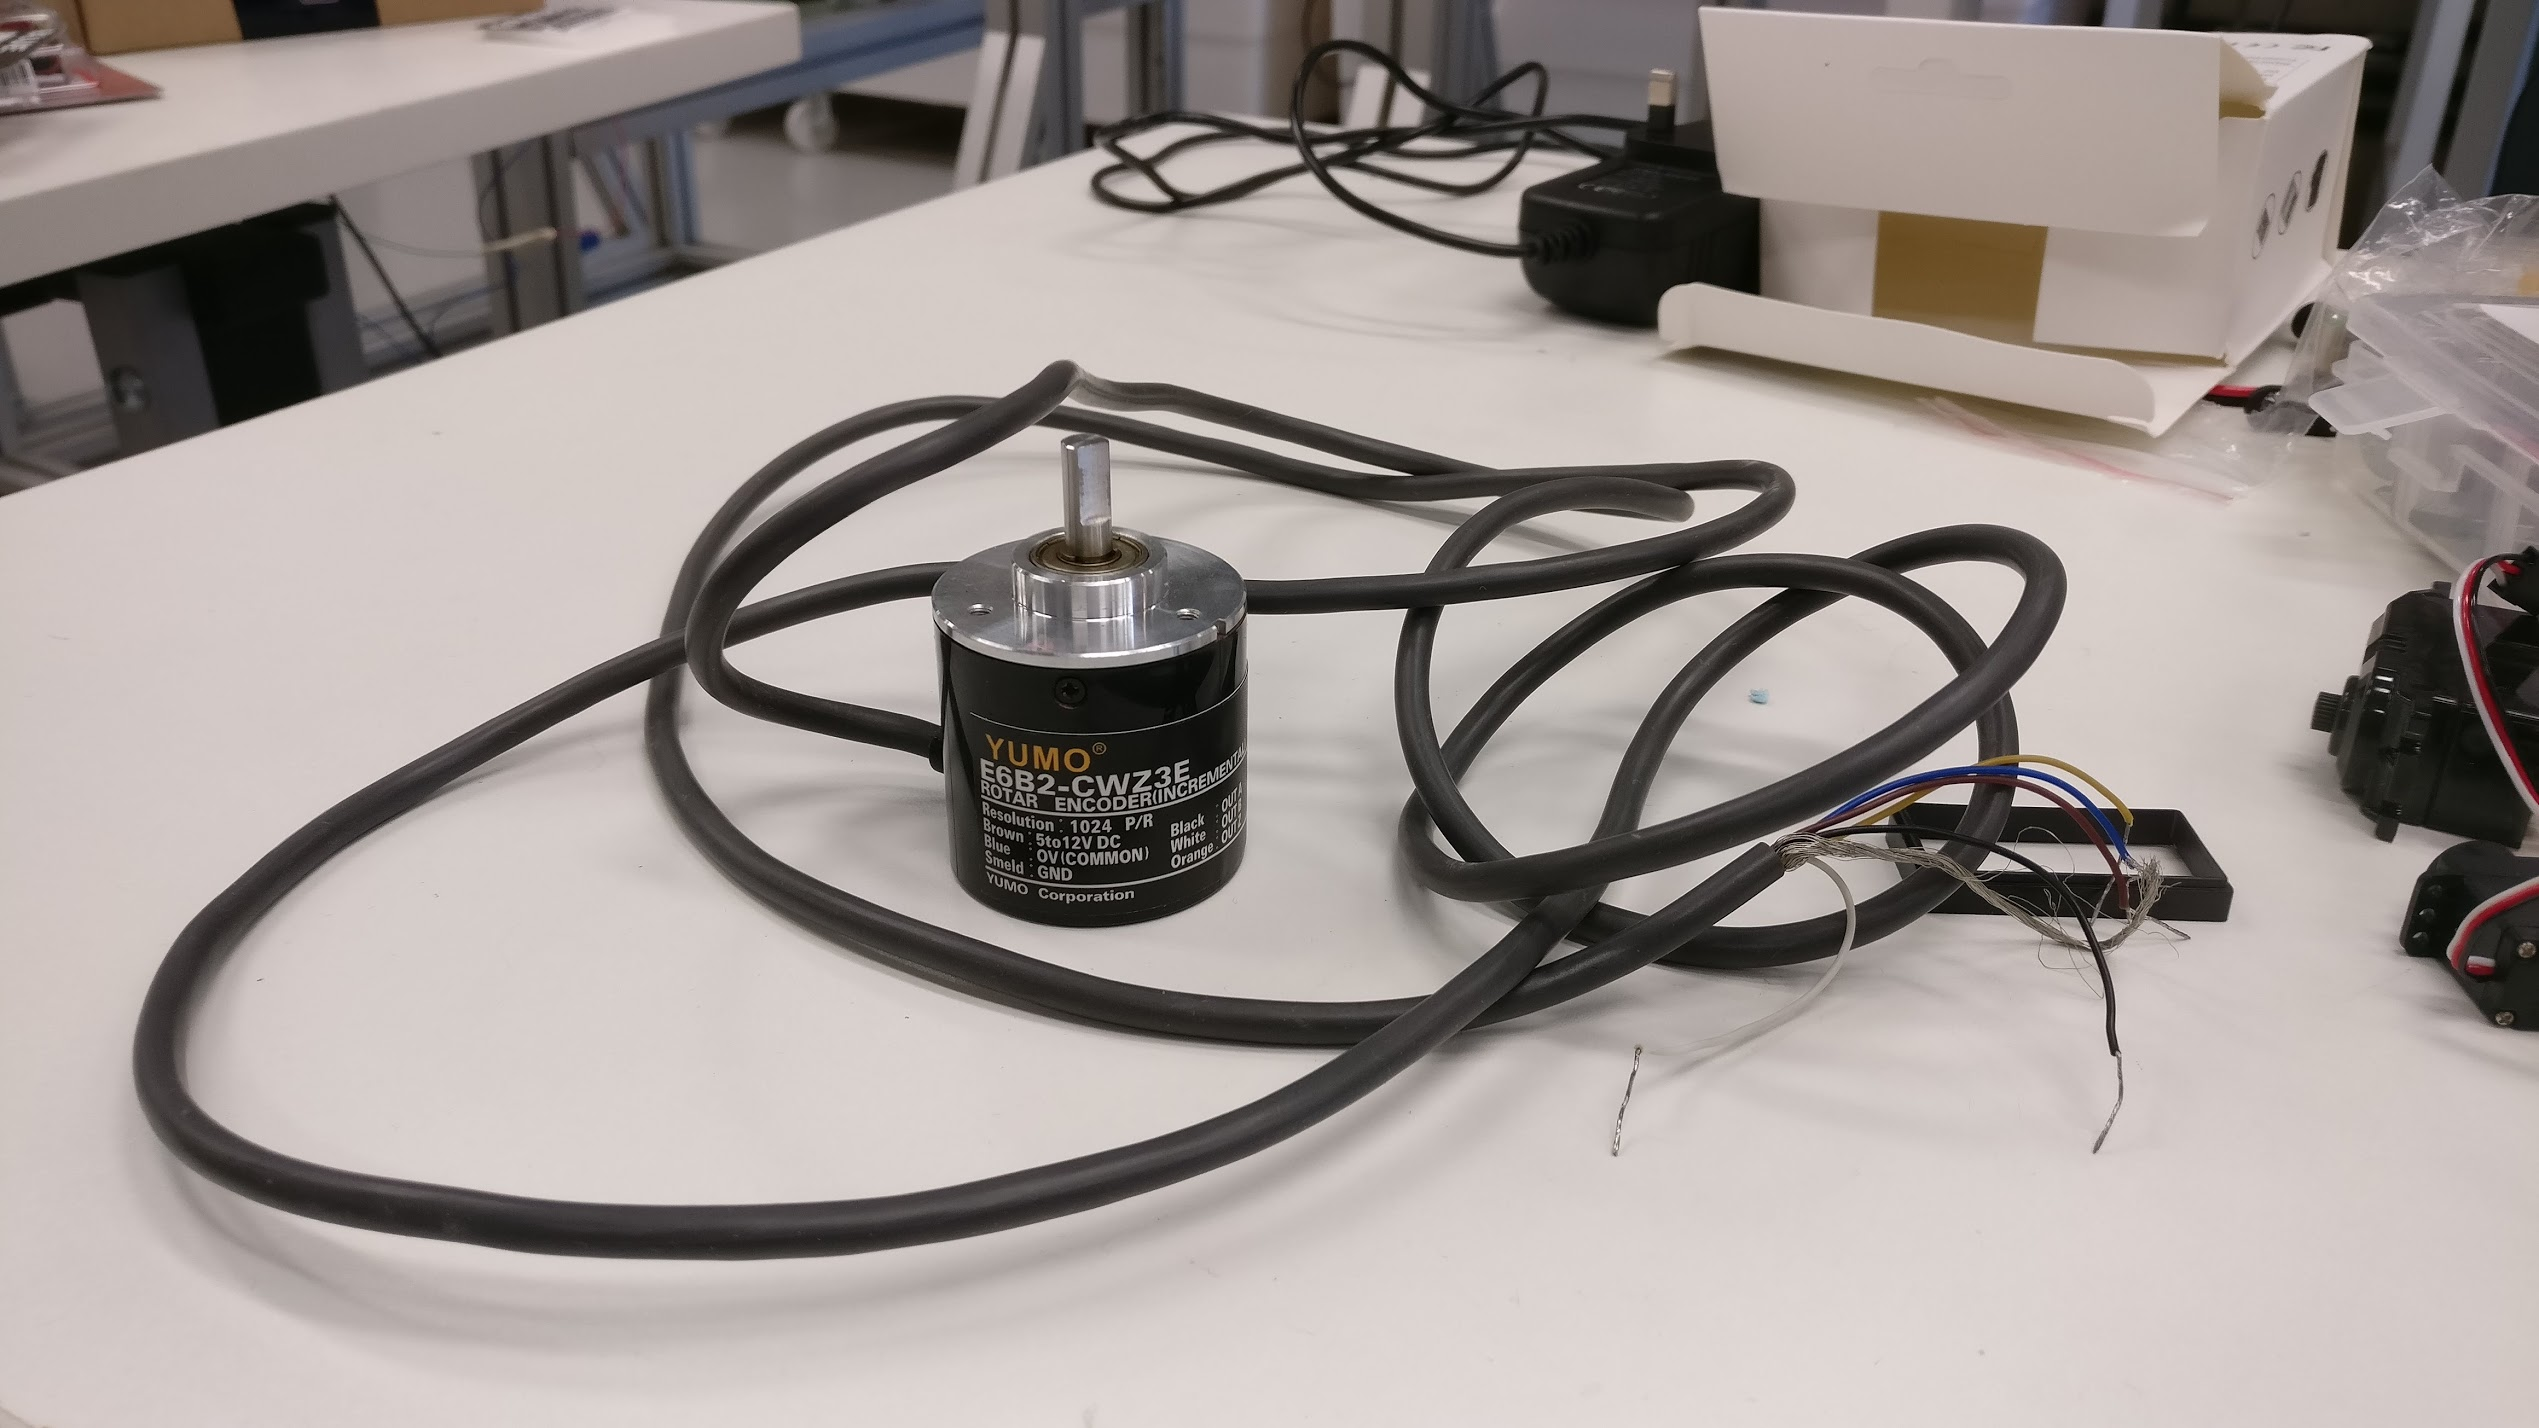
\includegraphics[scale=0.1]{rot.jpg}
\caption{YUMO E6B2-CWZ3E rotary encoder to record the angular position of servo}
\centering
\end{figure}
To measure the performance of the servo, a rotary encoder was used. This device converts the angular position into digital signals. The typical quadrature rotary encoders work using two signals: A and B. These are 90 degrees out-of-phase and operate on two logic levels. For clockwise rotation the A and B transition occurs in 4 phases: 

\begin{table}[h]
\centering
\caption{Phases of quadrature rotary encoders}
\thispagestyle{fancy}
\label{my-label}
\begin{tabular}{lll}
        & A & B \\
Phase 1 & 0 & 0 \\
Phase 2 & 0 & 1 \\
Phase 3 & 1 & 1 \\
Phase 4 & 1 & 0
\end{tabular}
\end{table}
Signals produced during anticlockwise rotation occur in exactly the opposite sequence: signal A leads signal B. 

Each phase change increments a counter. Each counter increment corresponds to a very small angular displacement. Thus, this device will be helpful to understand the dynamics of the servo. 

The rotary encoder was coupled to the servo and the step response was monitored. The highest point was assumed to be 120 degrees because the manufacturer claims that 120 degrees is the throw of the servo. The following graph shows how the angle changes with time. The initial part of the graph is linear which implies  that the servo has clearly reached the maximum speed it can achieve because the angular velocity is fairly constant. Right before the servo angle converges to the final value, the first order dynamics of the servo are visible. 
\begin{figure}[h]
\centering
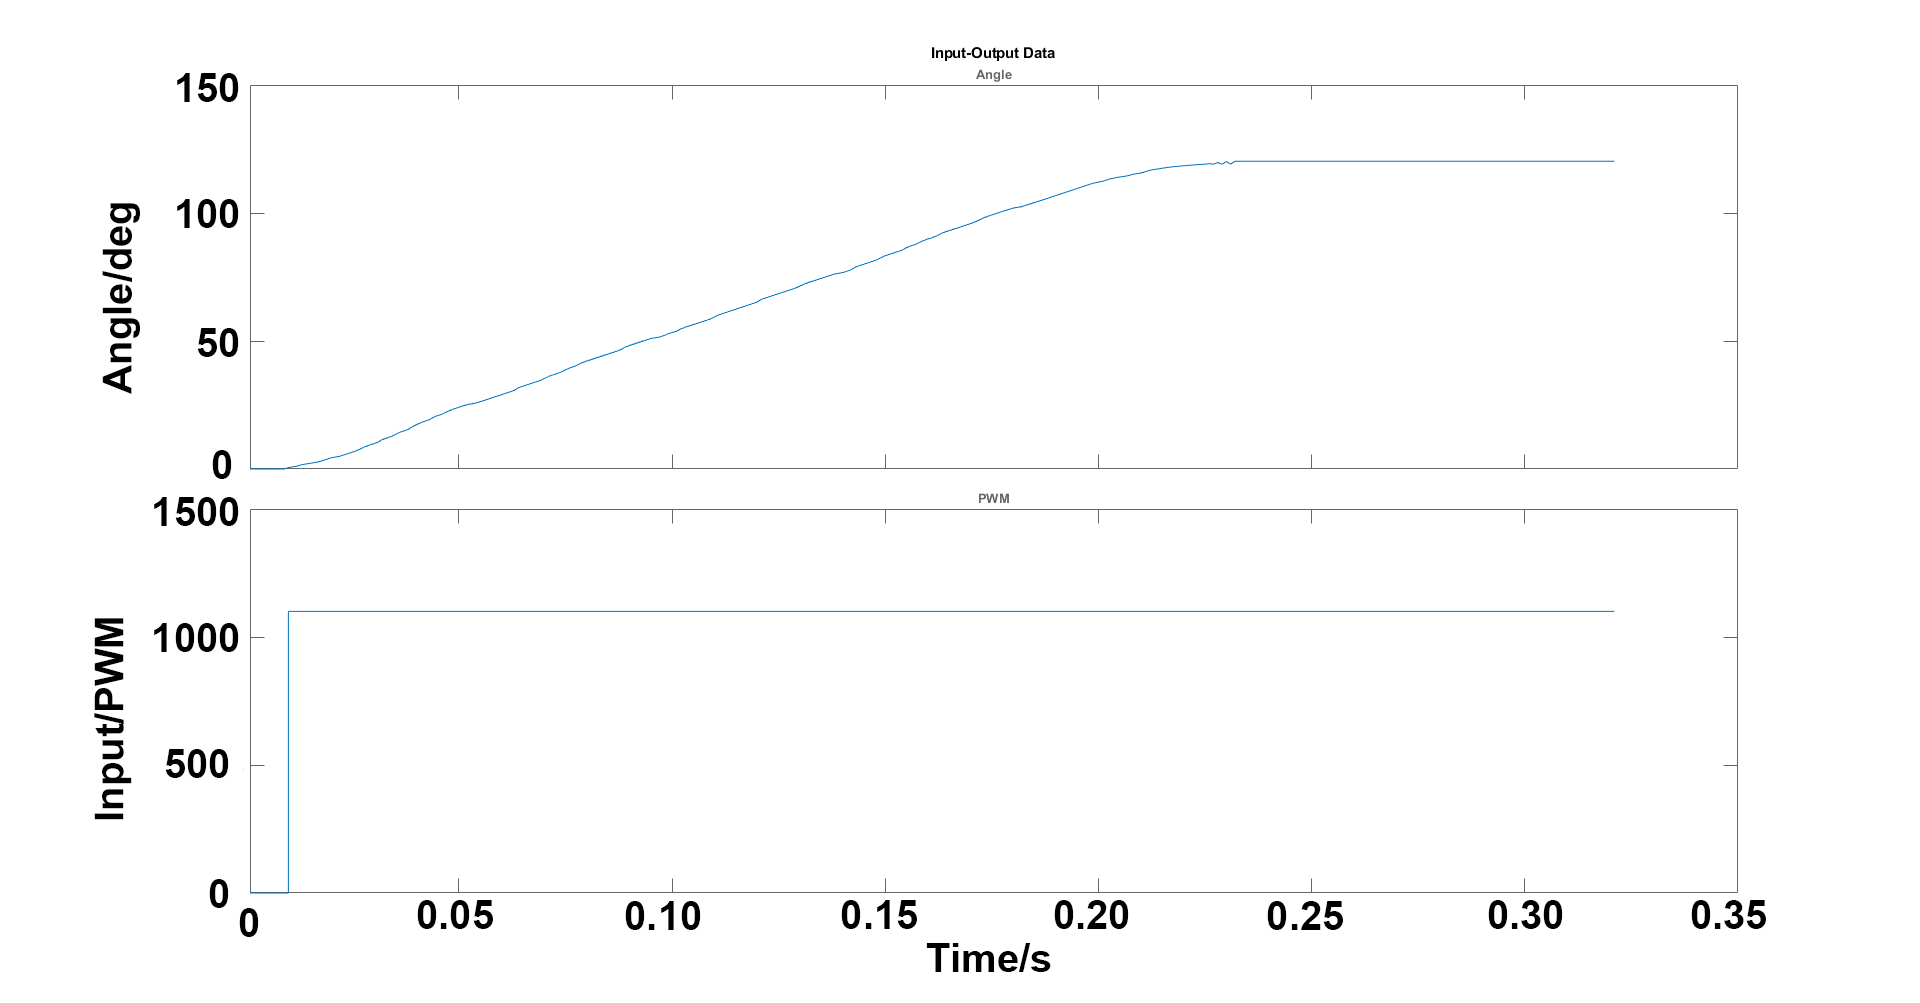
\includegraphics[scale=0.3]{iodat.png}
\caption{Step response of servo to an input of 1100 at around 0.01s.}
\centering
\end{figure}
\thispagestyle{fancy}
If that portion of the graph isolated and analysed how it converges, the time constant can be found assuming that the servo follows first order dynamics (simple lag) \cite{etkin}. 
\thispagestyle{fancy}
The following expression is the transfer function for a first order system. 
\begin{equation}
\frac{K}{Ts+1}
\end{equation}
\newpage
\thispagestyle{fancy}
When subjected to a step input $1/s$, the following transfer function is obtained.
\begin{equation}
\theta(s) = \frac{1100K}{s(Ts+1)}
\end{equation}

\thispagestyle{fancy}
This can be decompose into partial fractions.
\begin{equation}
\theta(s)=\frac{1100K}{s}-\frac{1100KT}{Ts+1}
\end{equation}


Then an inverse Laplace transform is applied to find the transfer function in the time domain. 
\begin{equation}
\mathcal{L}^{-1}\left(\frac{1100K}{s(Ts+1)}\right)=1100K(1-e^{\frac{t}{T}})
\end{equation}

According to the data collected, the servo reaches to 94.799$\%$ within 0.195s. So the time constant can be found. 

\begin{equation}
(1-e^{-0.195/T})=0.94799
\end{equation}

$$T=0.06596 s$$

\begin{figure}[H]
\centering
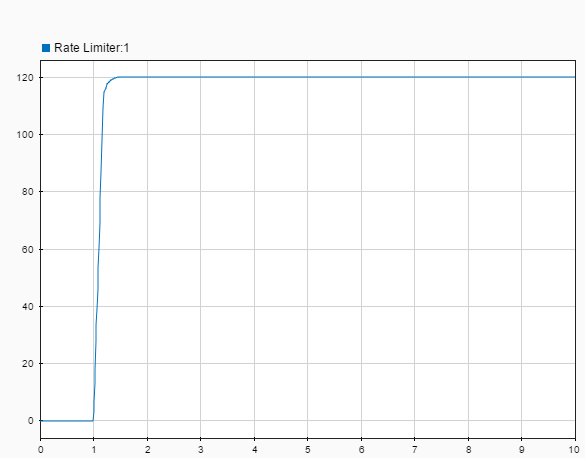
\includegraphics[scale=0.8]{servosim.png}
\caption{Servo approximation output in Simulink to a step input to displace servo from 0 to 120 deg.}
\centering
\end{figure}
The maximum speed can be found by taking the gradient at the straight line section of the graph.
\thispagestyle{fancy}
\begin{equation}
\dot{\theta}_{MAX}=0.599^{\circ}ms^{-1}
\end{equation}
Finally, the gain is simply the ratio between the output and the input which is 120/1100. 
\begin{equation}
K=0.10909
\end{equation}
This model of the servo gives a very close approximation of the real servo. A Simulink model of the servo was made which incorporates the first order transfer function and a rate limiter set to 599. When a step input of 1100 is applied to the system, the output (figure 5.4) matches the graph of the measured data as shown in figure 5.3.  


\section{Dynamics of the flap}
\begin{figure}[H]
\centering
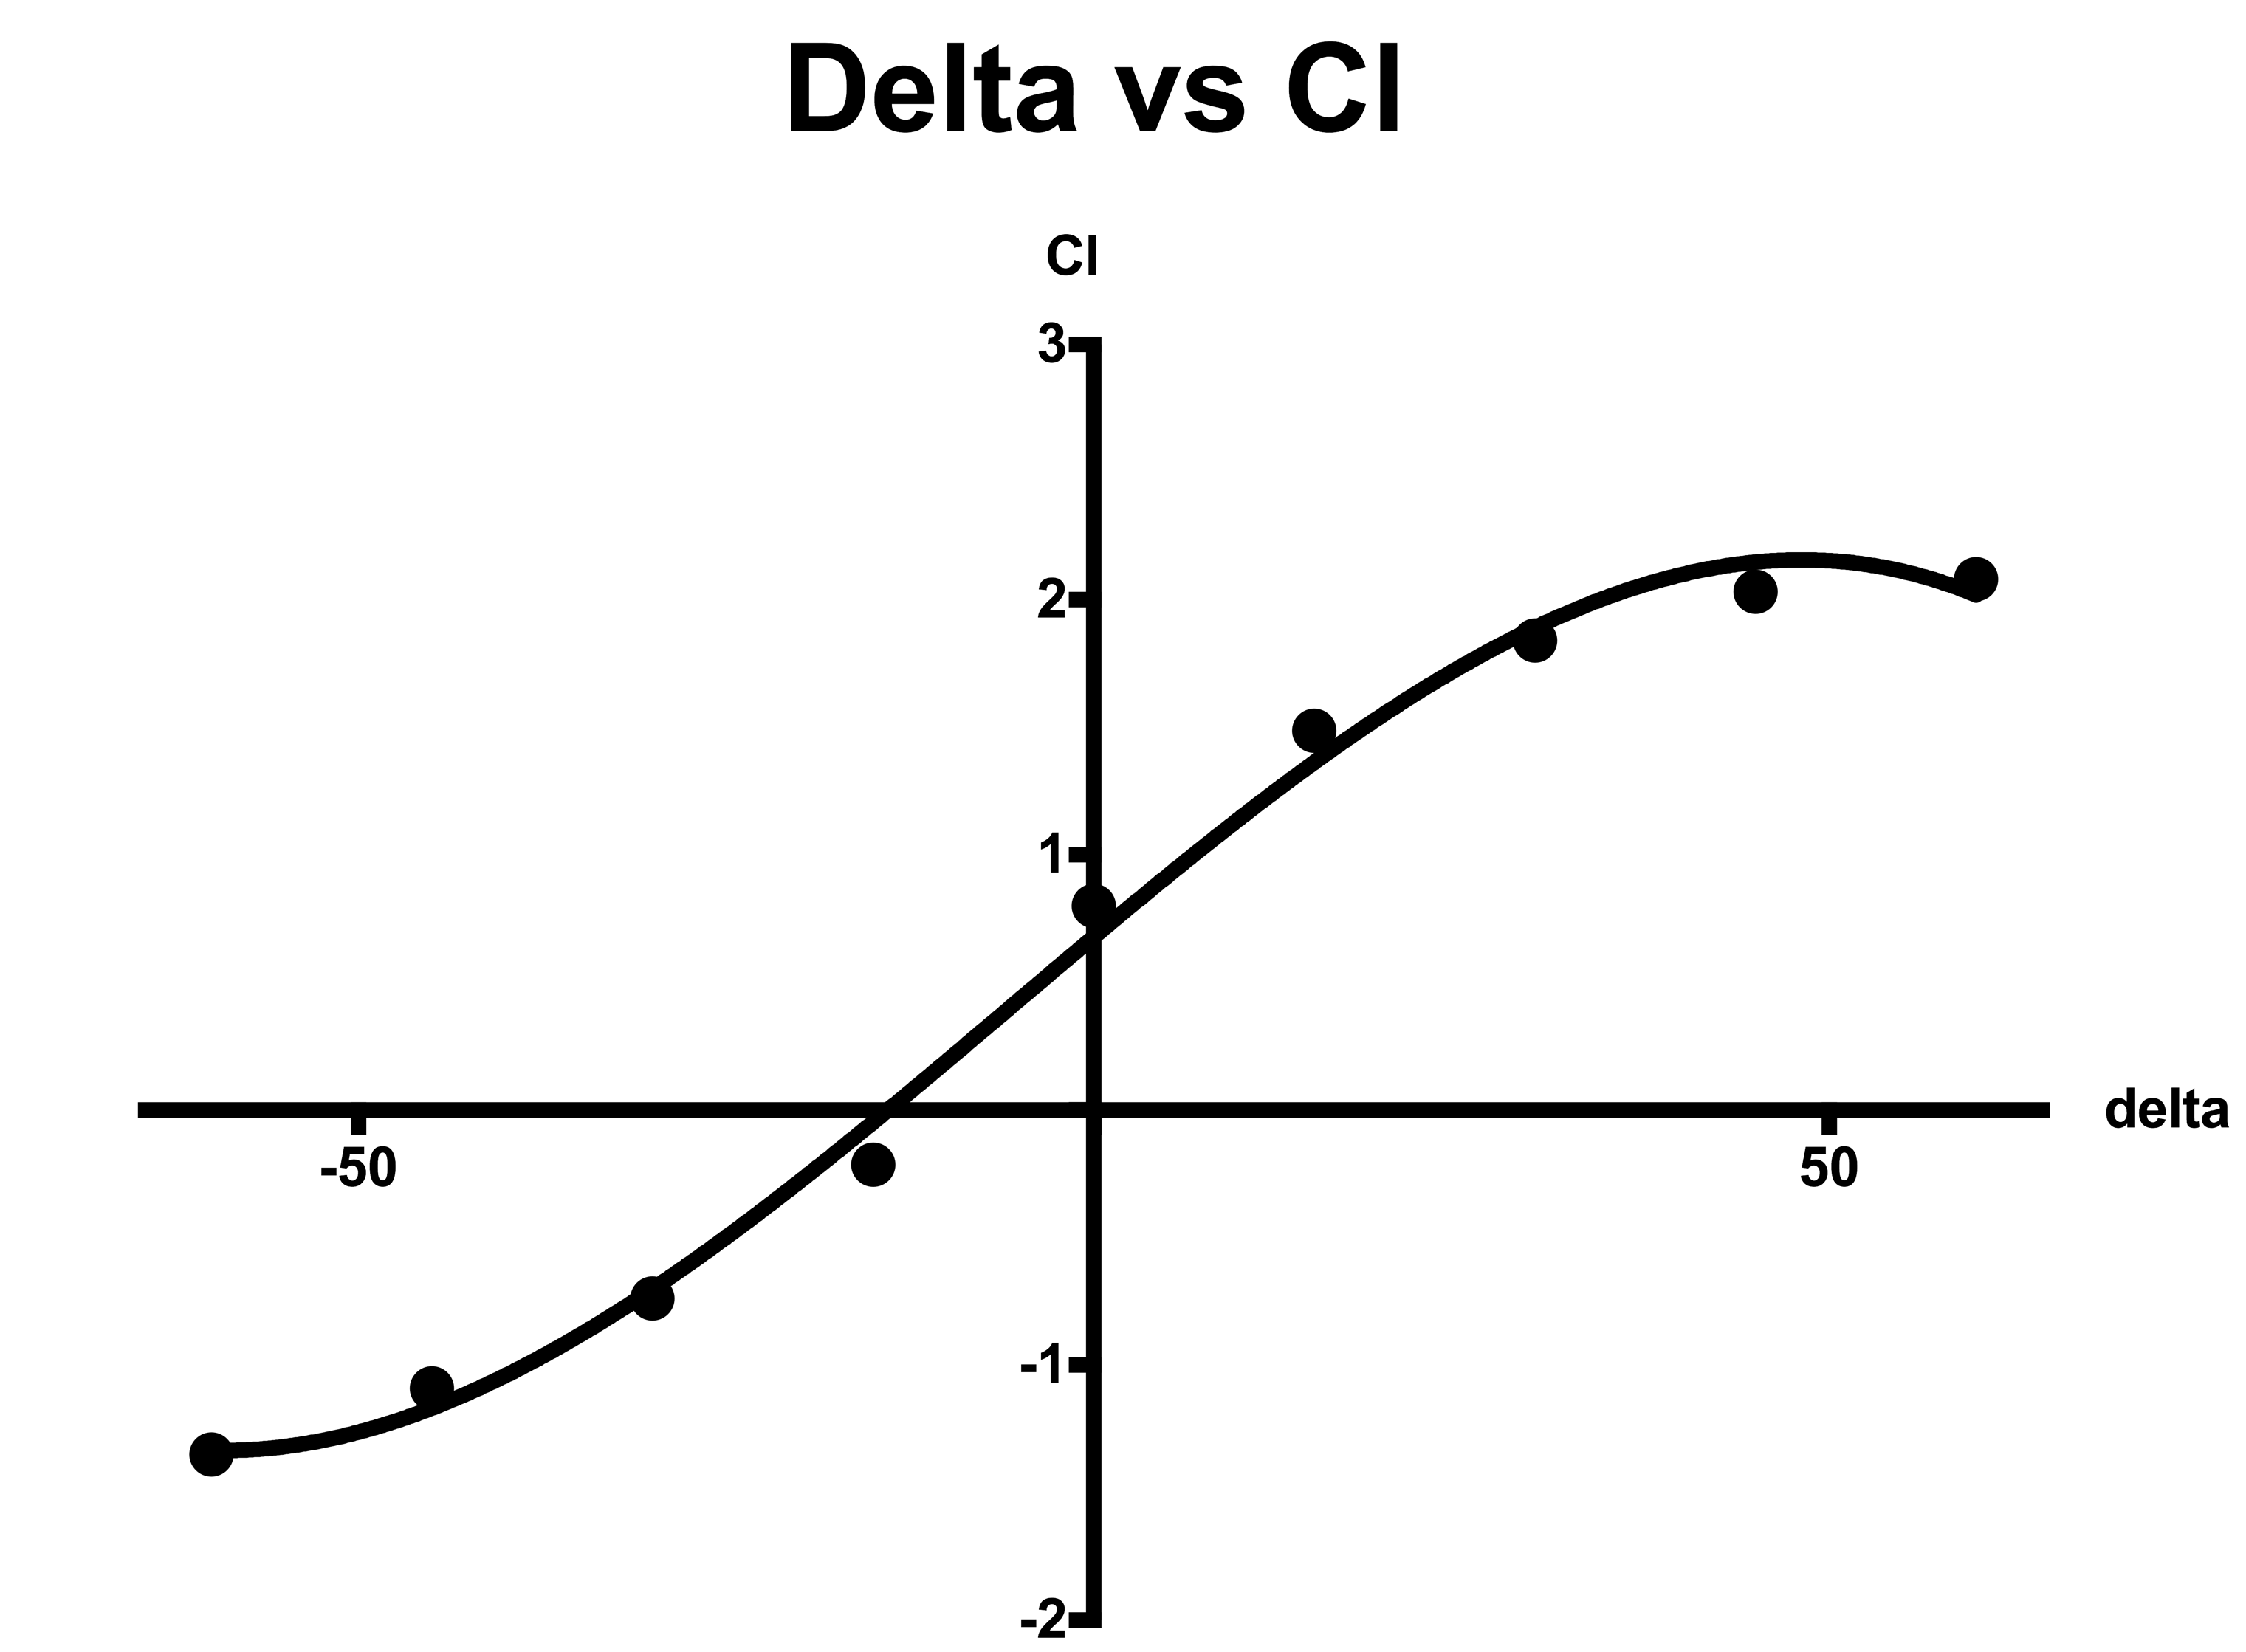
\includegraphics[scale=0.3]{dvcl.png}
\caption{Flap deflection vs Coefficient of Lift. The solid line is a cubic function.}
\centering
\end{figure}
\thispagestyle{fancy}
It is now known how the angular displacement of the flap changes with time. There is now a need to know how that change in angle affects the coefficient of lift and consequently the lift. 

To do this, Xfoil was used to see how the $C_{L}$ changes with deflection of the flap.

The graphing software shows that a cubic function is a good fit for the data. However, a cubic function was not used to approximate the flap dynamics because at the maximum/minimum point, it is not clear which direction the flap must deflect to increase/decrease the lift coefficient. 

A better approximation is a linear function with saturation on both ends because it is monotonic. There is no ambiguity in which way the flap needs to deflect to increase/decrease $C_{L}$. 


\begin{equation}
C_{L}(\delta)=0.04257\delta+0.6665
\end{equation}
\begin{equation}
-1.35\leq C_{L}\leq2.08
\end{equation}


\section{Simulink first principles modelling}
\thispagestyle{fancy}
The last two sections identified the dynamics of the plant. It is now possible to import the models developed into Simulink and use the PID tuner app in MATLAB to tune controller for output disturbance rejection (impulse in output). 
\begin{figure}[H]
\centering
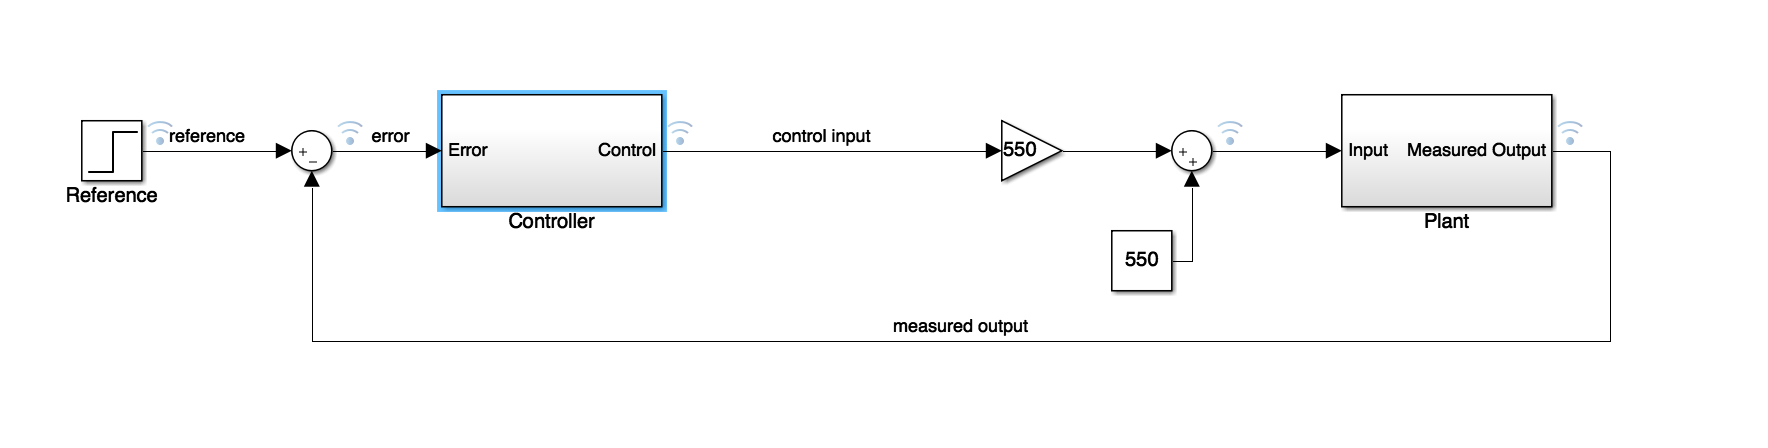
\includegraphics[scale=0.5]{simu.png}
\caption{Simulink model. Note that the PID output signal is converted to a PWM value before entering the plant.}
\centering
\end{figure}
The image below is a screenshot of the Simulink model. The reference signal is a step signal that has a magnitude of 3.2 from 0s. The error signal is converted to a command signal or a 'control input' which ranges from -1 to 1. -1 corresponds to the flap being all the way up (-60 deg) which requires a PWM input of 0. On the other hand, for deflecting the flap all the way down (60 deg) a PWM value of 1100 is sent. 

Therefore, to convert the controller output to a PWM output, a gain of 550 is applied and a constant 550 is added. 

The PWM signal is consequently fed into the plant. 
\thispagestyle{fancy}
\begin{figure}[H]
\centering
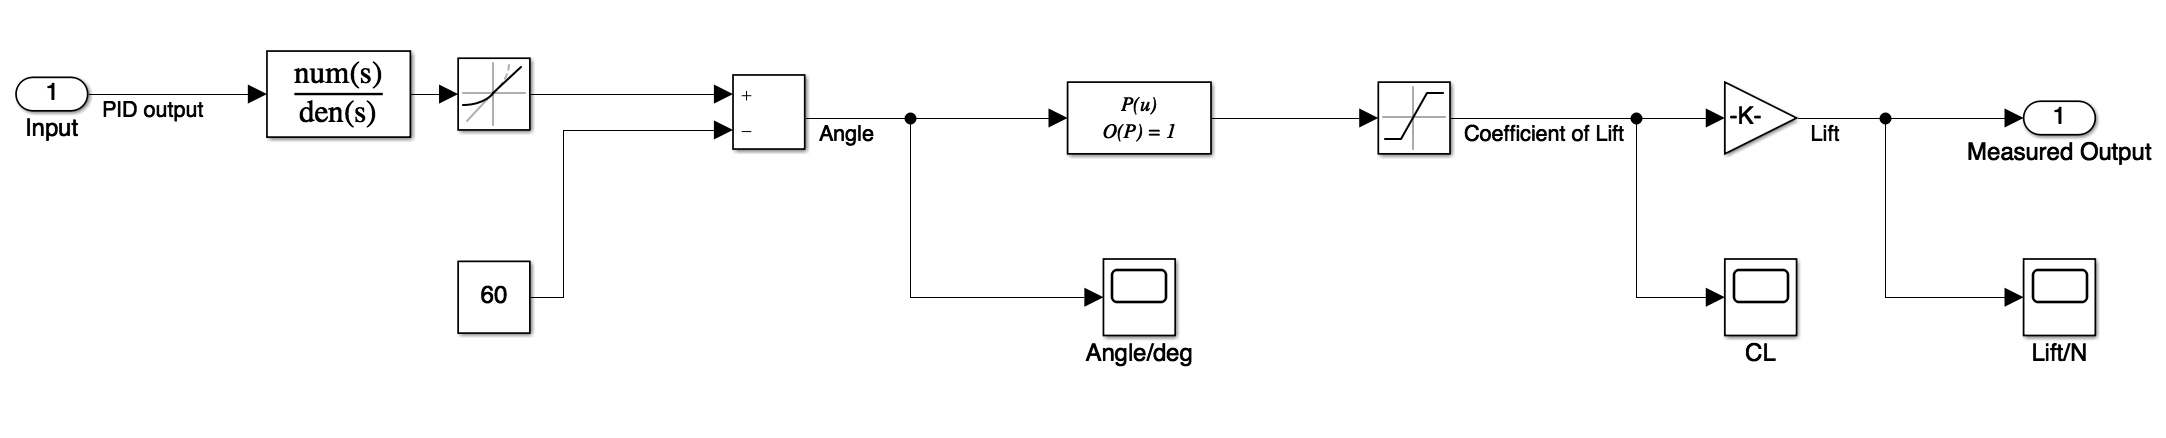
\includegraphics[scale=0.40]{plants.png}
\caption{Simulink model of the plant. The control signal enters as a PWM value and the output of the whole plant is the lift (process variable)}
\centering
\end{figure}
\thispagestyle{fancy} 
In figure 5.7, on the far left the controller generated PWM signal comes in. This goes through a transfer function and a rate limiter as outlined in section 5.2. The output is the flap deflection angle. This signal then goes through a first order polynomial (refer to eq 5.8 and 5.9). The output is the coefficient of lift. This can be converted to lift by applying a gain of 6.615. 
\begin{equation}
L=\frac{1}{2}\rho V^{2}SC_{L} = \frac{1}{2} \cdot 1.225 \cdot 12^{2} \cdot 0.30 \cdot 0.25 \cdot C_{L} = 6.615C_{L}
\end{equation}

This completes the model that was used for tuning the controller. To begin testing, the software will calculate the optimum PID gains.

 

\begin{figure}[H]
\centering
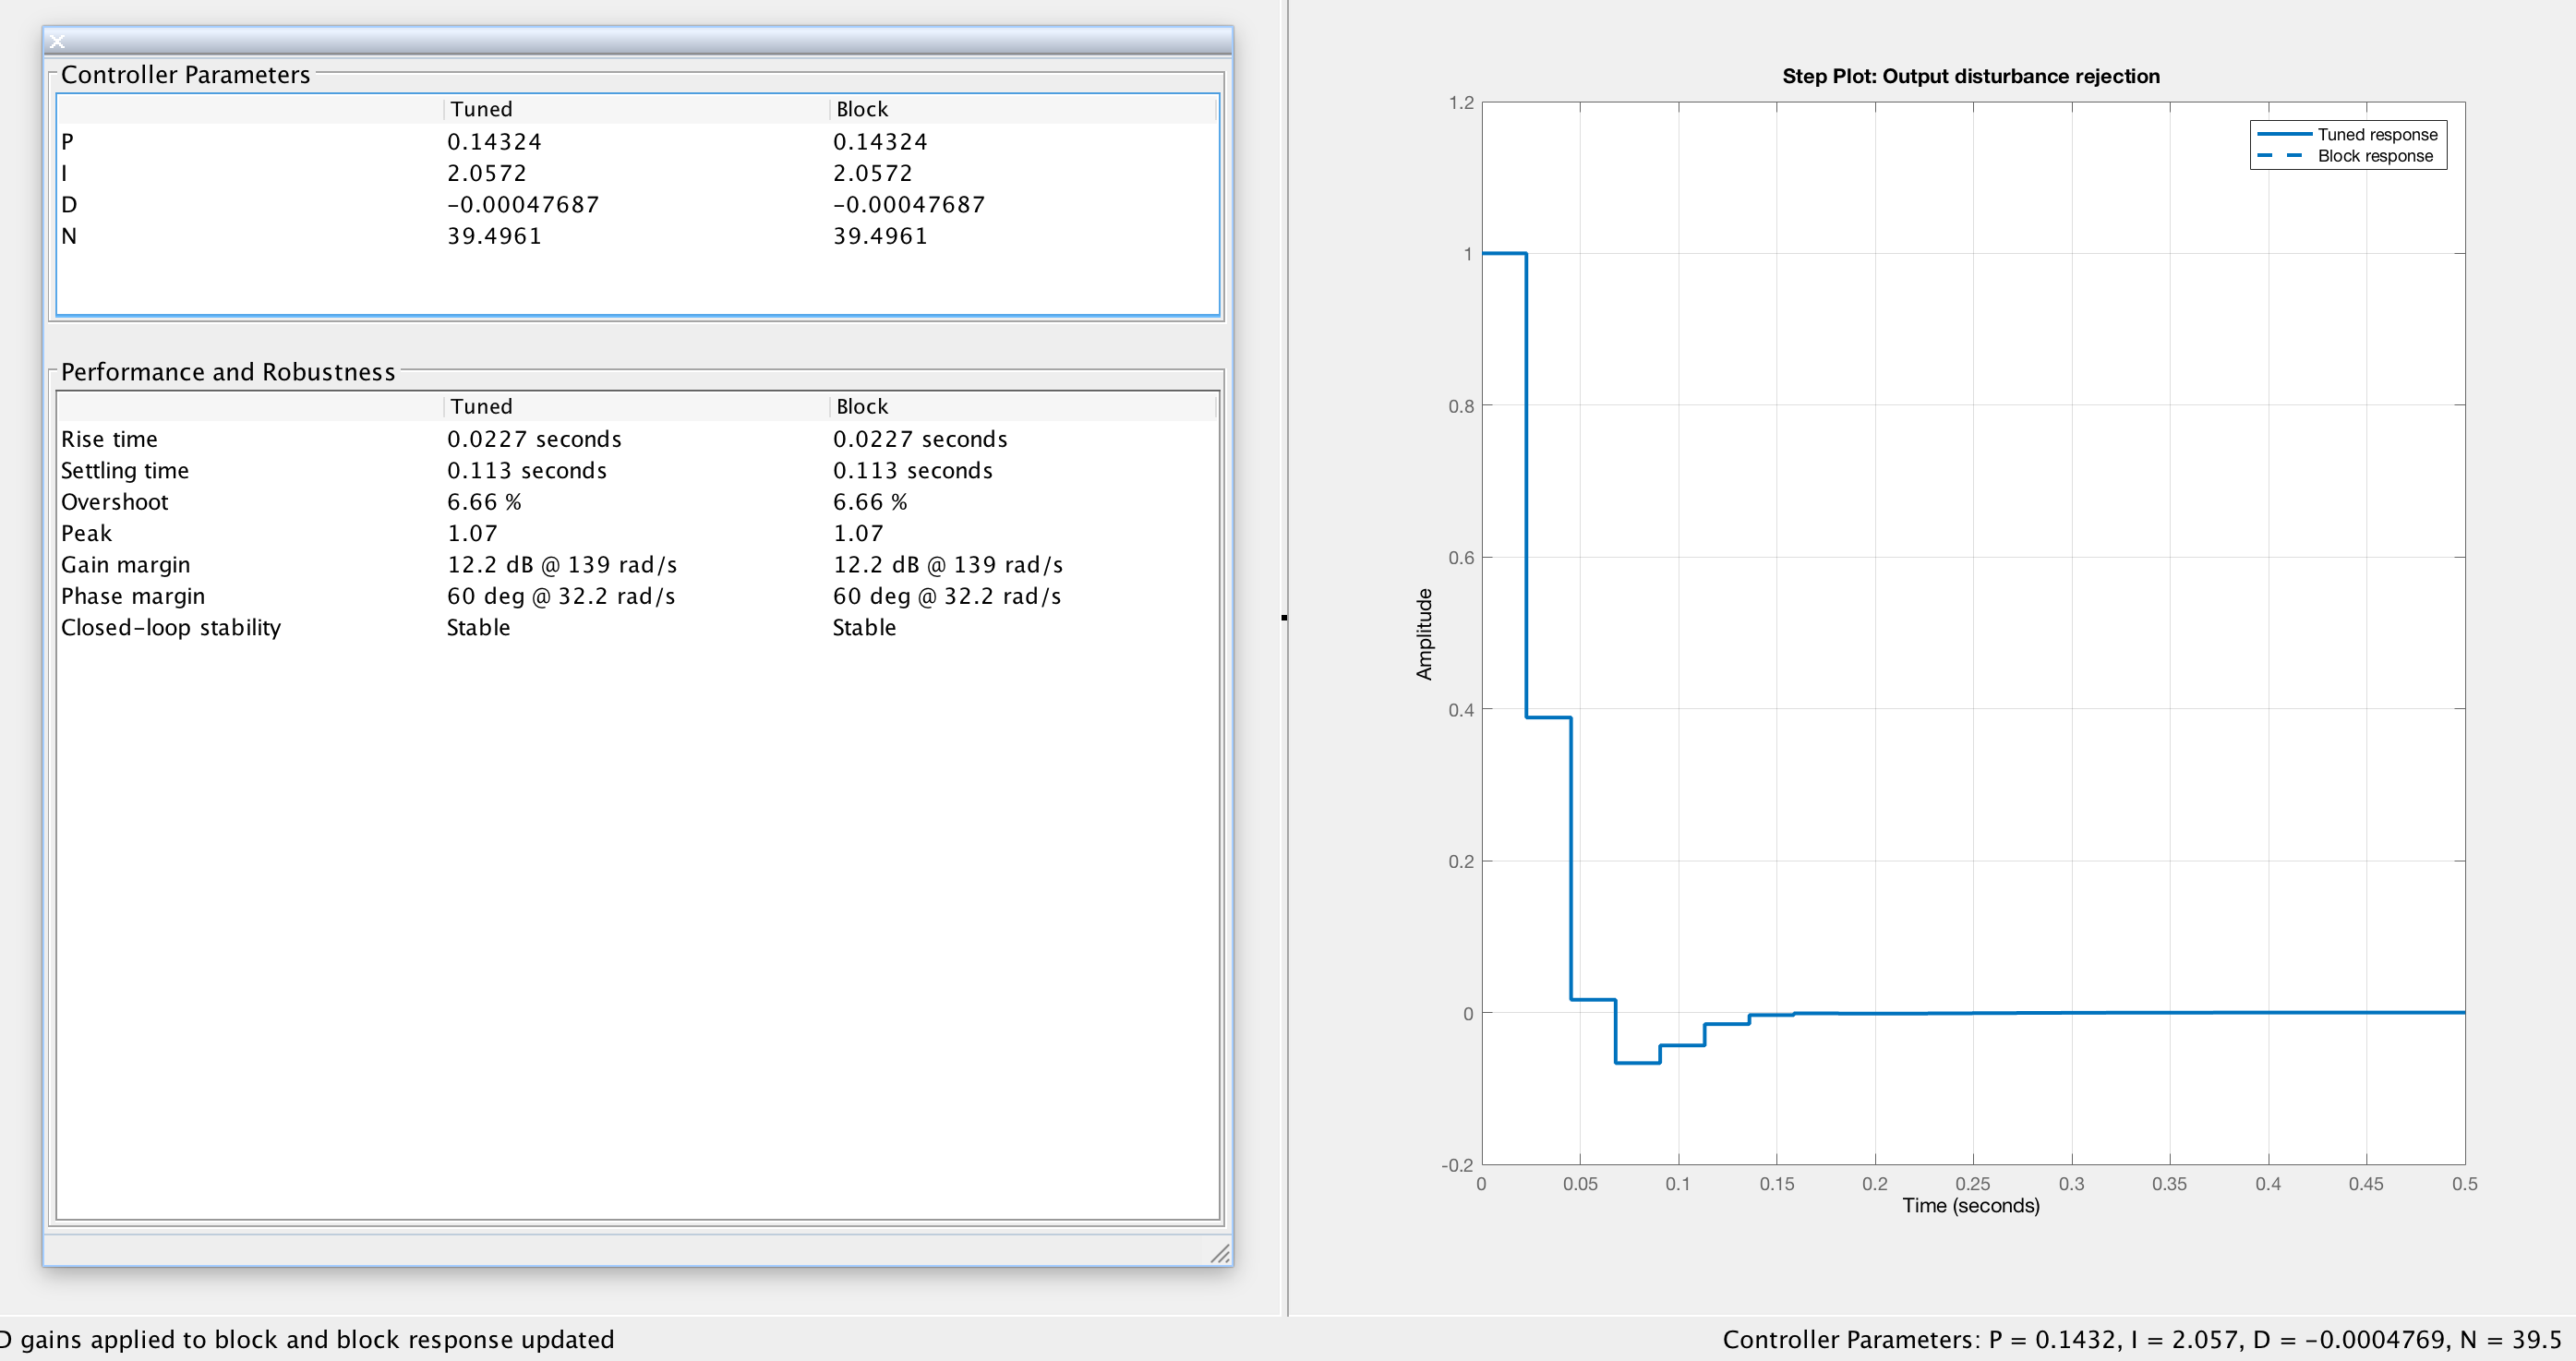
\includegraphics[scale=0.32]{pidt.png}
\caption{Tuner app with the performance parameters and the optimised gains in the bottom right}
\centering
\end{figure}
As mentioned earlier, the PID tuner app in MATLAB was used to determine these gains. 

The optimisation process was started by tracking the output disturbance rejection plot (gust) and then adjusting the response time until it was under 0.13s. The percentage overshoot was kept under 10$\%$ by adjusting the robustness of the system. The optimal gains found are shown in the table below. 
\begin{table}[H]
\centering
\caption{Matlab predicted PID gains}
\label{my-label}
\begin{tabular}{ll}
$K_{p}$ & 0.14324     \\
$K_{i}$ & 2.0572      \\
$K_{d}$ & -0.00047687
\end{tabular}
\end{table}
\thispagestyle{fancy} 
\chapter{Lift estimation and implementation}
\section{Lift Estimation}
\thispagestyle{fancy}
In chapter 3, pressure in pascals was obtained from the pressure sensors. This section will deal with using the pressure data from the sensors to calculate the lift produced by the wing. A good lift estimate is essential for feedback. 
\newline
\newline
Lift and drag are both aerodynamic forces that are a result of an unequal pressure (thus force) distribution along the surface of the wing. If the force due to pressure normal to the direction of the free stream is resolved, the result would be the lift on the wing. Similarly, the component of pressure forces parallel to the free stream is resolved to find the drag. 
\begin{equation}
\overrightarrow{F_{N}}=\oint{p{\hat{\textbf{n}}}}dS
\end{equation}
\begin{equation}
L=\overrightarrow{F_{N}}\cdot\hat{\textbf{n}}\cos\alpha
\end{equation}
\begin{equation}
D=\overrightarrow{F_{N}}\cdot\hat{\textbf{n}}\sin\alpha
\end{equation}
These equations cannot be directly applied to measured data because there are pressure readings over finite discrete points along the wing surface. But if the wing has a large number of pressure tappings, the lift can be estimated by just summing the product of the individual pressure readings and the distance between consecutive tappings. 
\begin{equation}
L=\sum_{i=1}^{n}{(p_{li}-p_{ui})}\delta A
\end{equation}
Linear interpolation between consecutive points can further improve the estimation.
\newline
\newline 
\thispagestyle{fancy}
The size of the wing in this project is unfortunately constrained due to the dimensions of the wind tunnel. Fitting a large number of pressure tappings within the wing was therefore not possible. A large number of pressure tappings also require a large number of pressure sensors which is not economically viable. So the lift estimation is expected to be a very rough approximation but the error should be under $10\%$. An empirical approach was used instead for this problem. 
\newline
\newline
It can be assumed that the lift is estimated by the following equation:
\begin{equation}
L=\sum_{i=1}^{3}{w_{i}(p_{li}-p_{ui})}
\end{equation}
$w_{1}$,$w_{2}$ and$w_{3}$ are weights given to the differential pressure readings from each location on the wing. These weights will be determined using Xfoil and Excel. 
\thispagestyle{fancy}
Xfoil was used to sweep through $\alpha$ between -5 and 10 and $\delta$ between $-60^{\circ}$ and $60^{\circ}$. The coefficient of pressure at $C_{p}$ at the top and bottom of the wing at x/c values of the pressure tappings will be recorded. These can be converted to pressure.
\begin{equation}
p=p_{\infty}+\frac{1}{2}\rho V_{\infty}^{2} C_{p}
\end{equation}

The pressure values should roughly be what the pressure sensors will actually measure. The $C_{L}$ is also recorded for each test. This can be used to find the actual lift on the wing. 
\newline
\newline
The results were all entered into an excel spreadsheet. A column for the estimated lift took the xfoil predicted pressure at each tapping, multiplied it by the corresponding weight and added them. The square of the error was calculated by taking the difference between the actual lift and the estimated lift and squaring the resulting value. 
\newline
\newline
Excel has a solver function which is carries out an optimisation routine. The sum of the squared error values for all tests (across all angles of attacks and flap deflections) was minimised by allowing the solver to adjust the weights. 
\thispagestyle{fancy}
The following values were determined by excel solver. The average percentage error was about $7.3\%$.
\begin{table}[h]
\label{my-label}
\begin{tabular}{ll}
$w_{1}$ & 0.021042611     \\
$w_{2}$ & -0.022570784      \\
$w_{3}$ & 0.025133973
\end{tabular}
\end{table}
\newline
\newline
Considering a wide range of flap deflection angles and angle-of-attack when estimating the weightings gave me a lift estimator that works fairly well for different operating conditions the system is likely to see during testing.   
The full Excel spreadsheet can be found in the appendix. 
\newpage
\section{Implementing the controller}
\thispagestyle{fancy}
\begin{wrapfigure}{r}{0.5\textwidth}
  \begin{center}
    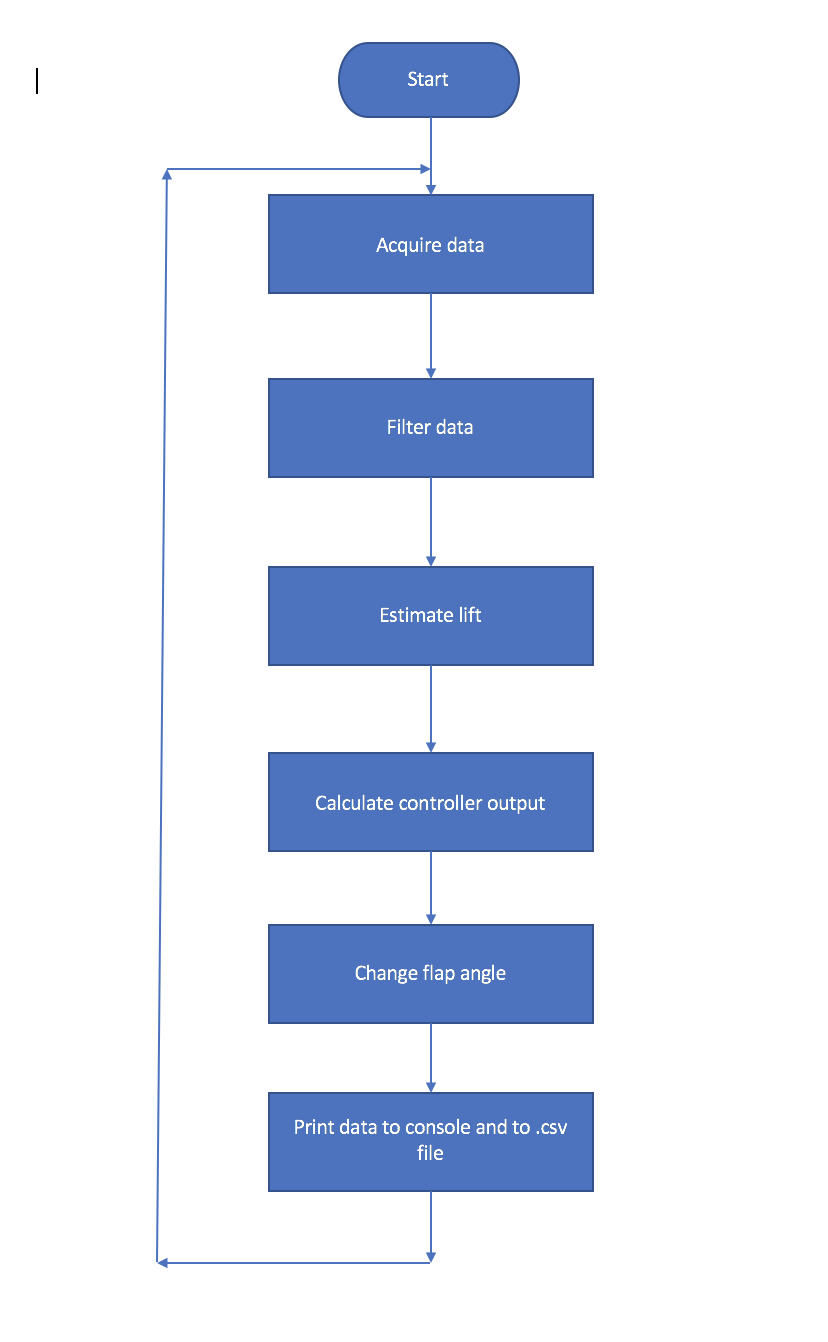
\includegraphics[width=0.48\textwidth]{flow.png}
  \end{center}
  \caption{Flowchart showing the sequence of code blocks}
\end{wrapfigure}
Before testing can begin, the code has to be written that will collect the data from the sensors and use it to calculate the lift. It should then control the flap angle in accordance to the controller that was designed in the preceding chapter. 

Figure 6.1 shows the sequence of tasks that need to be carried out when the code is compiled and executed. The 'main' function in my code ran an iterative loop that called different functions, each with a dedicated purpose. Roughly each block in figure 6.1 had its own function.  The main function was also used to set up the I2C devices and the servo. Both the I2C devices and the servo were implemented using the wiringPi and wiringPiI2C libraries both of which are made publicly available by Gordon\cite{gordon} under GNU LGPLv3 license. 
\newline
\newline
\newline
The iterative loop mentioned above was done via an endless while loop as given below. The 'clockgettime' function was called at the beginning and the end of the loop to calculate the loop/sample time which is useful for the PID calculation and also to understand whether the program was running fast enough to keep up with the oscillation. 
\begin{lstlisting}[style=CStyle]
	while(1){
		clock_gettime(CLOCK_REALTIME, &gettime_now);
		start_time = gettime_now.tv_nsec;
		counter+=1; 
		daq(fd, fd2); //acquire data from sensors and filter them
		estimateLift(); //estimate lift
		control(); //run a PID iteration
		printdata(); //record data and print to console
		clock_gettime(CLOCK_REALTIME, &gettime_now);
		if(gettime_now.tv_nsec - start_time>0){
			dt = (gettime_now.tv_nsec - start_time)/1000000000;
		}
	}
\end{lstlisting}
\thispagestyle{fancy}
The 'control' function was responsible for the PID calculations. There is a high probability of integral wind-up during initialisation and gust tests because the error temporarily will be very high. The prolonged saturation caused can lead to the integral error accumulating to a very large value. This can cause the output of the controller to stay saturated long after the cause of the error has gone away. 
\newline
\newline
Anti-windup protection can help avoid this. The output of the controller is clamped to the maximum/minimum value and nothing is added to the integral error term until the output is within the acceptable range. The code can be found in its entirety in appendix E. 
\thispagestyle{fancy}
\chapter{Wind tunnel testing}
\thispagestyle{fancy}
All the tools, equipment and resources required for the project have been gathered and assembled as discussed in the preceding chapters. This chapter will outline how the testing was carried out in chronological order. As with most things, the first iteration of any design is likely to be flawed. But this chapter will show how the system was improved and optimised the in each successive iteration.   
\section{Measuring wind tunnel airspeed}
The wind tunnel is operated using a control panel which displayed a frequency. This frequency is proportional to the airspeed in the wind tunnel. However, the exact relation between this frequency and the airspeed was unknown. Thus, the speed of the wind tunnel had to be measured at different frequencies to make sure that the airspeed was kept at 12 meters per second since this was assumed when designing the lift estimator.

Using a pitot probe and one of the differential pressure sensors a clear linear relation between the frequency and the airspeed could be seen. The following figure shows this relation. 
\begin{figure}[H]
\centering
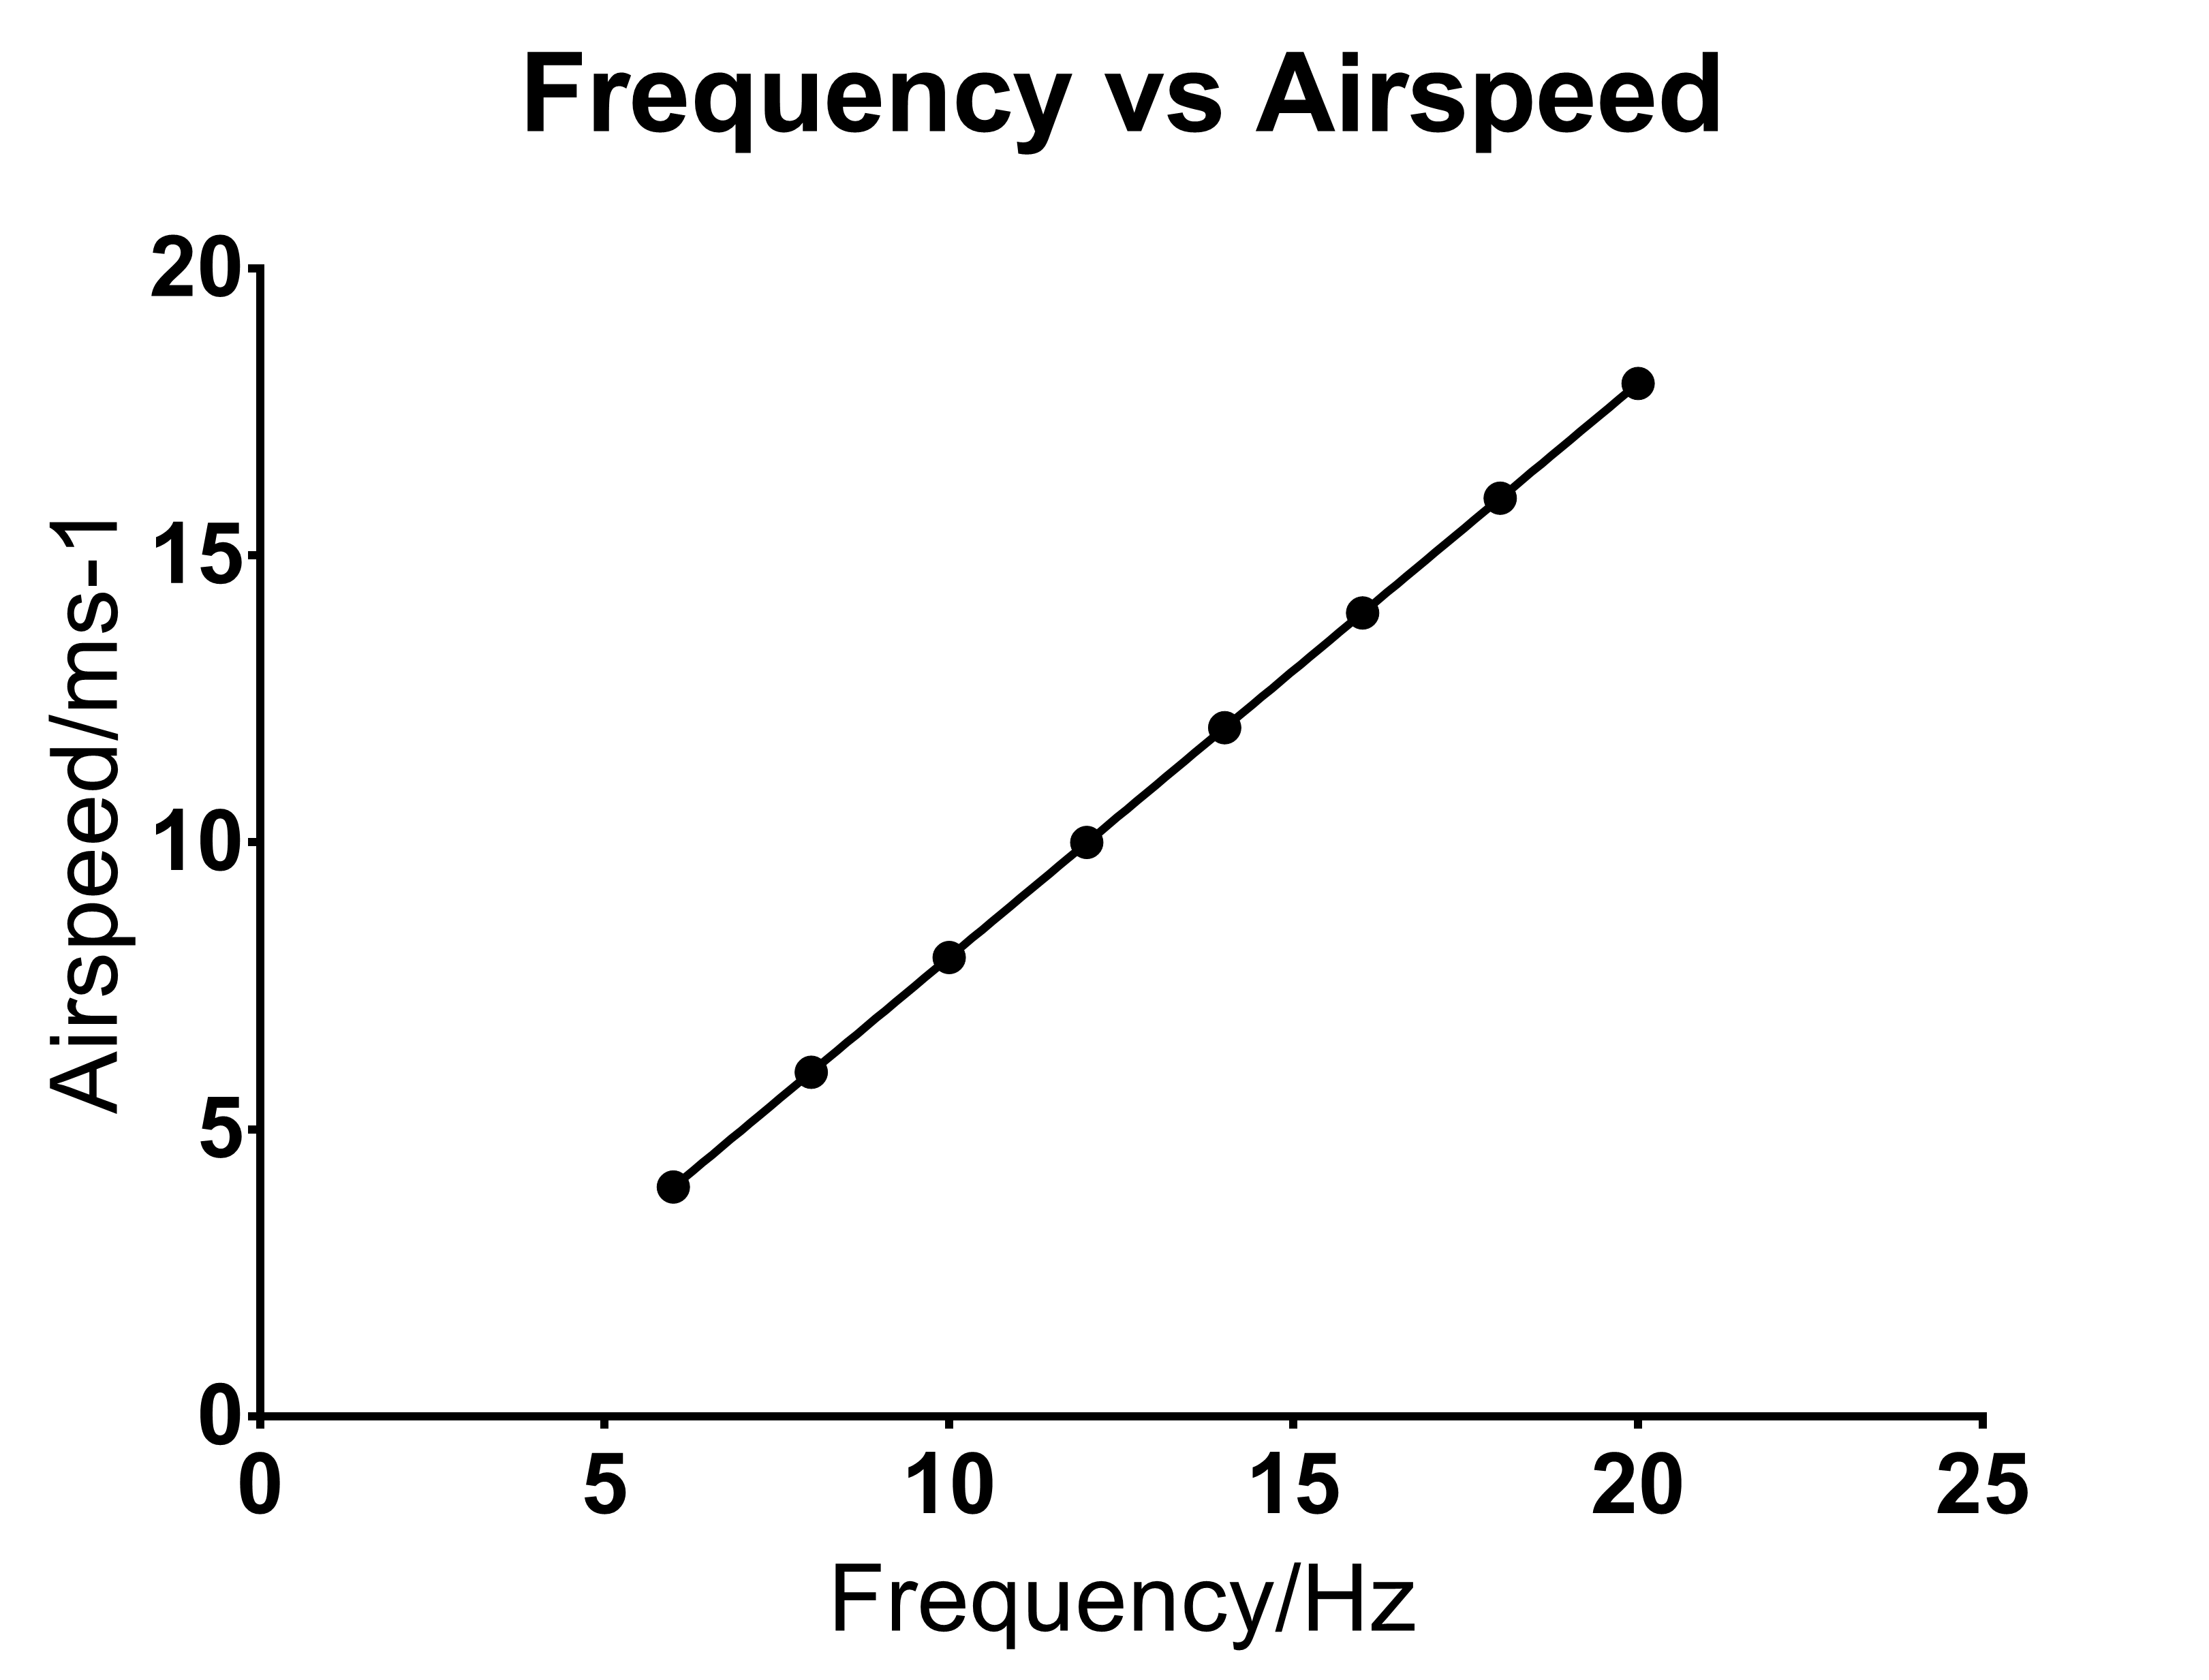
\includegraphics[width=0.6\textwidth,center]{wtu.png}
\caption{Relation between the frequency and the airspeed in the wind tunnel}
\centering
\end{figure}

To keep the test conditions constant, all tests will be run  at a constant speed of $12ms^{-1}$ (except the airspeed sweep test). The angle of attack will be kept at $5^{\circ}$ which according to the lift estimator should give me a lift of 4.6 N. The setpoint will be at 3.2N. 

\section{First test}
\thispagestyle{fancy}
It was logical to test the control system at steady conditions before moving on to the gust tests. The wind tunnel was set to $12ms^{-1}$. The controller should be able to hold the lift at roughly 3.2N. 
\begin{figure}[H]
\centering
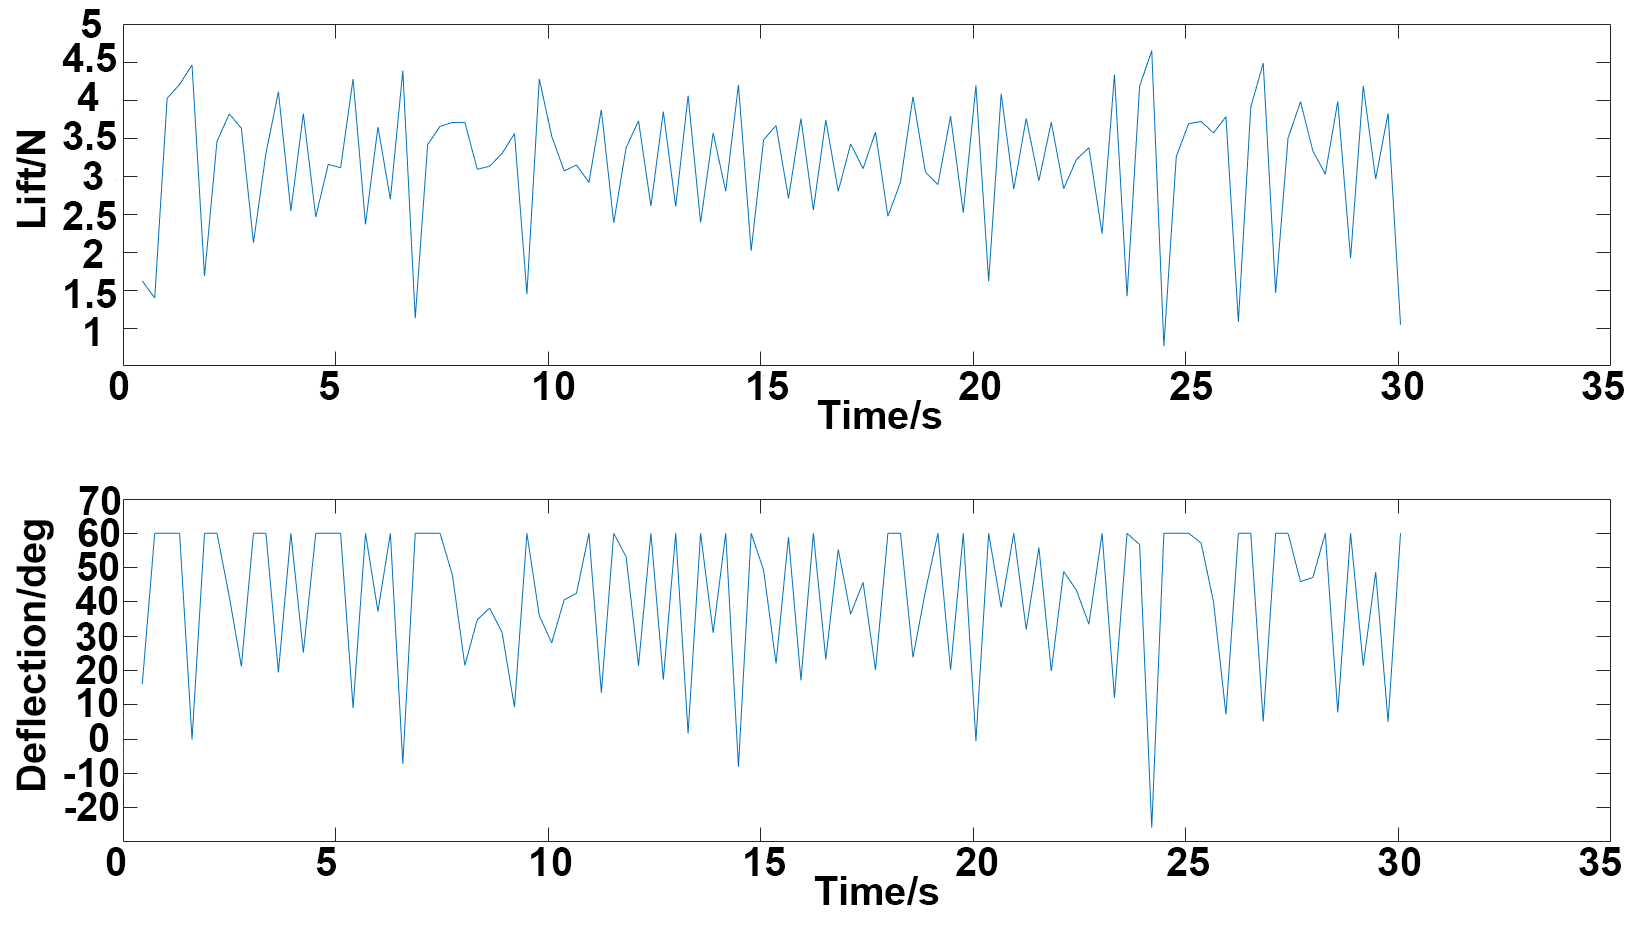
\includegraphics[width=1\textwidth,left]{osc.png}
\caption{The controller was unable to converge the lift to the setpoint. Controller is tuned too aggressively.}
\centering
\end{figure}


The above result was expected. The controller was unable to stabilise the system and oscillated violently. As you can see from figure 7.2, the flap angle repeatedly saturated at $60^{\circ}$ (flap down position). This was expected because the controller was tuned very aggressively. There is also a considerable amount of noise in the data to which the controller was hypersensitive. One solution to this issue would be to increase the averaging window size to reduce noise. However, this would mean that the sample rate decreases below the Nyquist frequency. It may also mask the gust to the point where the impulse will go undetected. 
\thispagestyle{fancy}

In order to fix the controller, a different approach was used. By considering the system response to a specific input, the plant can be approximated and the appropriate gains can be found. A heuristic method called Cohen and Coon\cite{cohen} tuning helped improve the system.
\newpage  
\section{Cohen and Coon tuning}
\thispagestyle{fancy}
This method involves using the plant in open loop. A step input is given to the system and the output is monitored. A step input from -60 degrees to 60 degrees was applied to the system and the figure below shows the response. 
\begin{figure}[H]
\centering
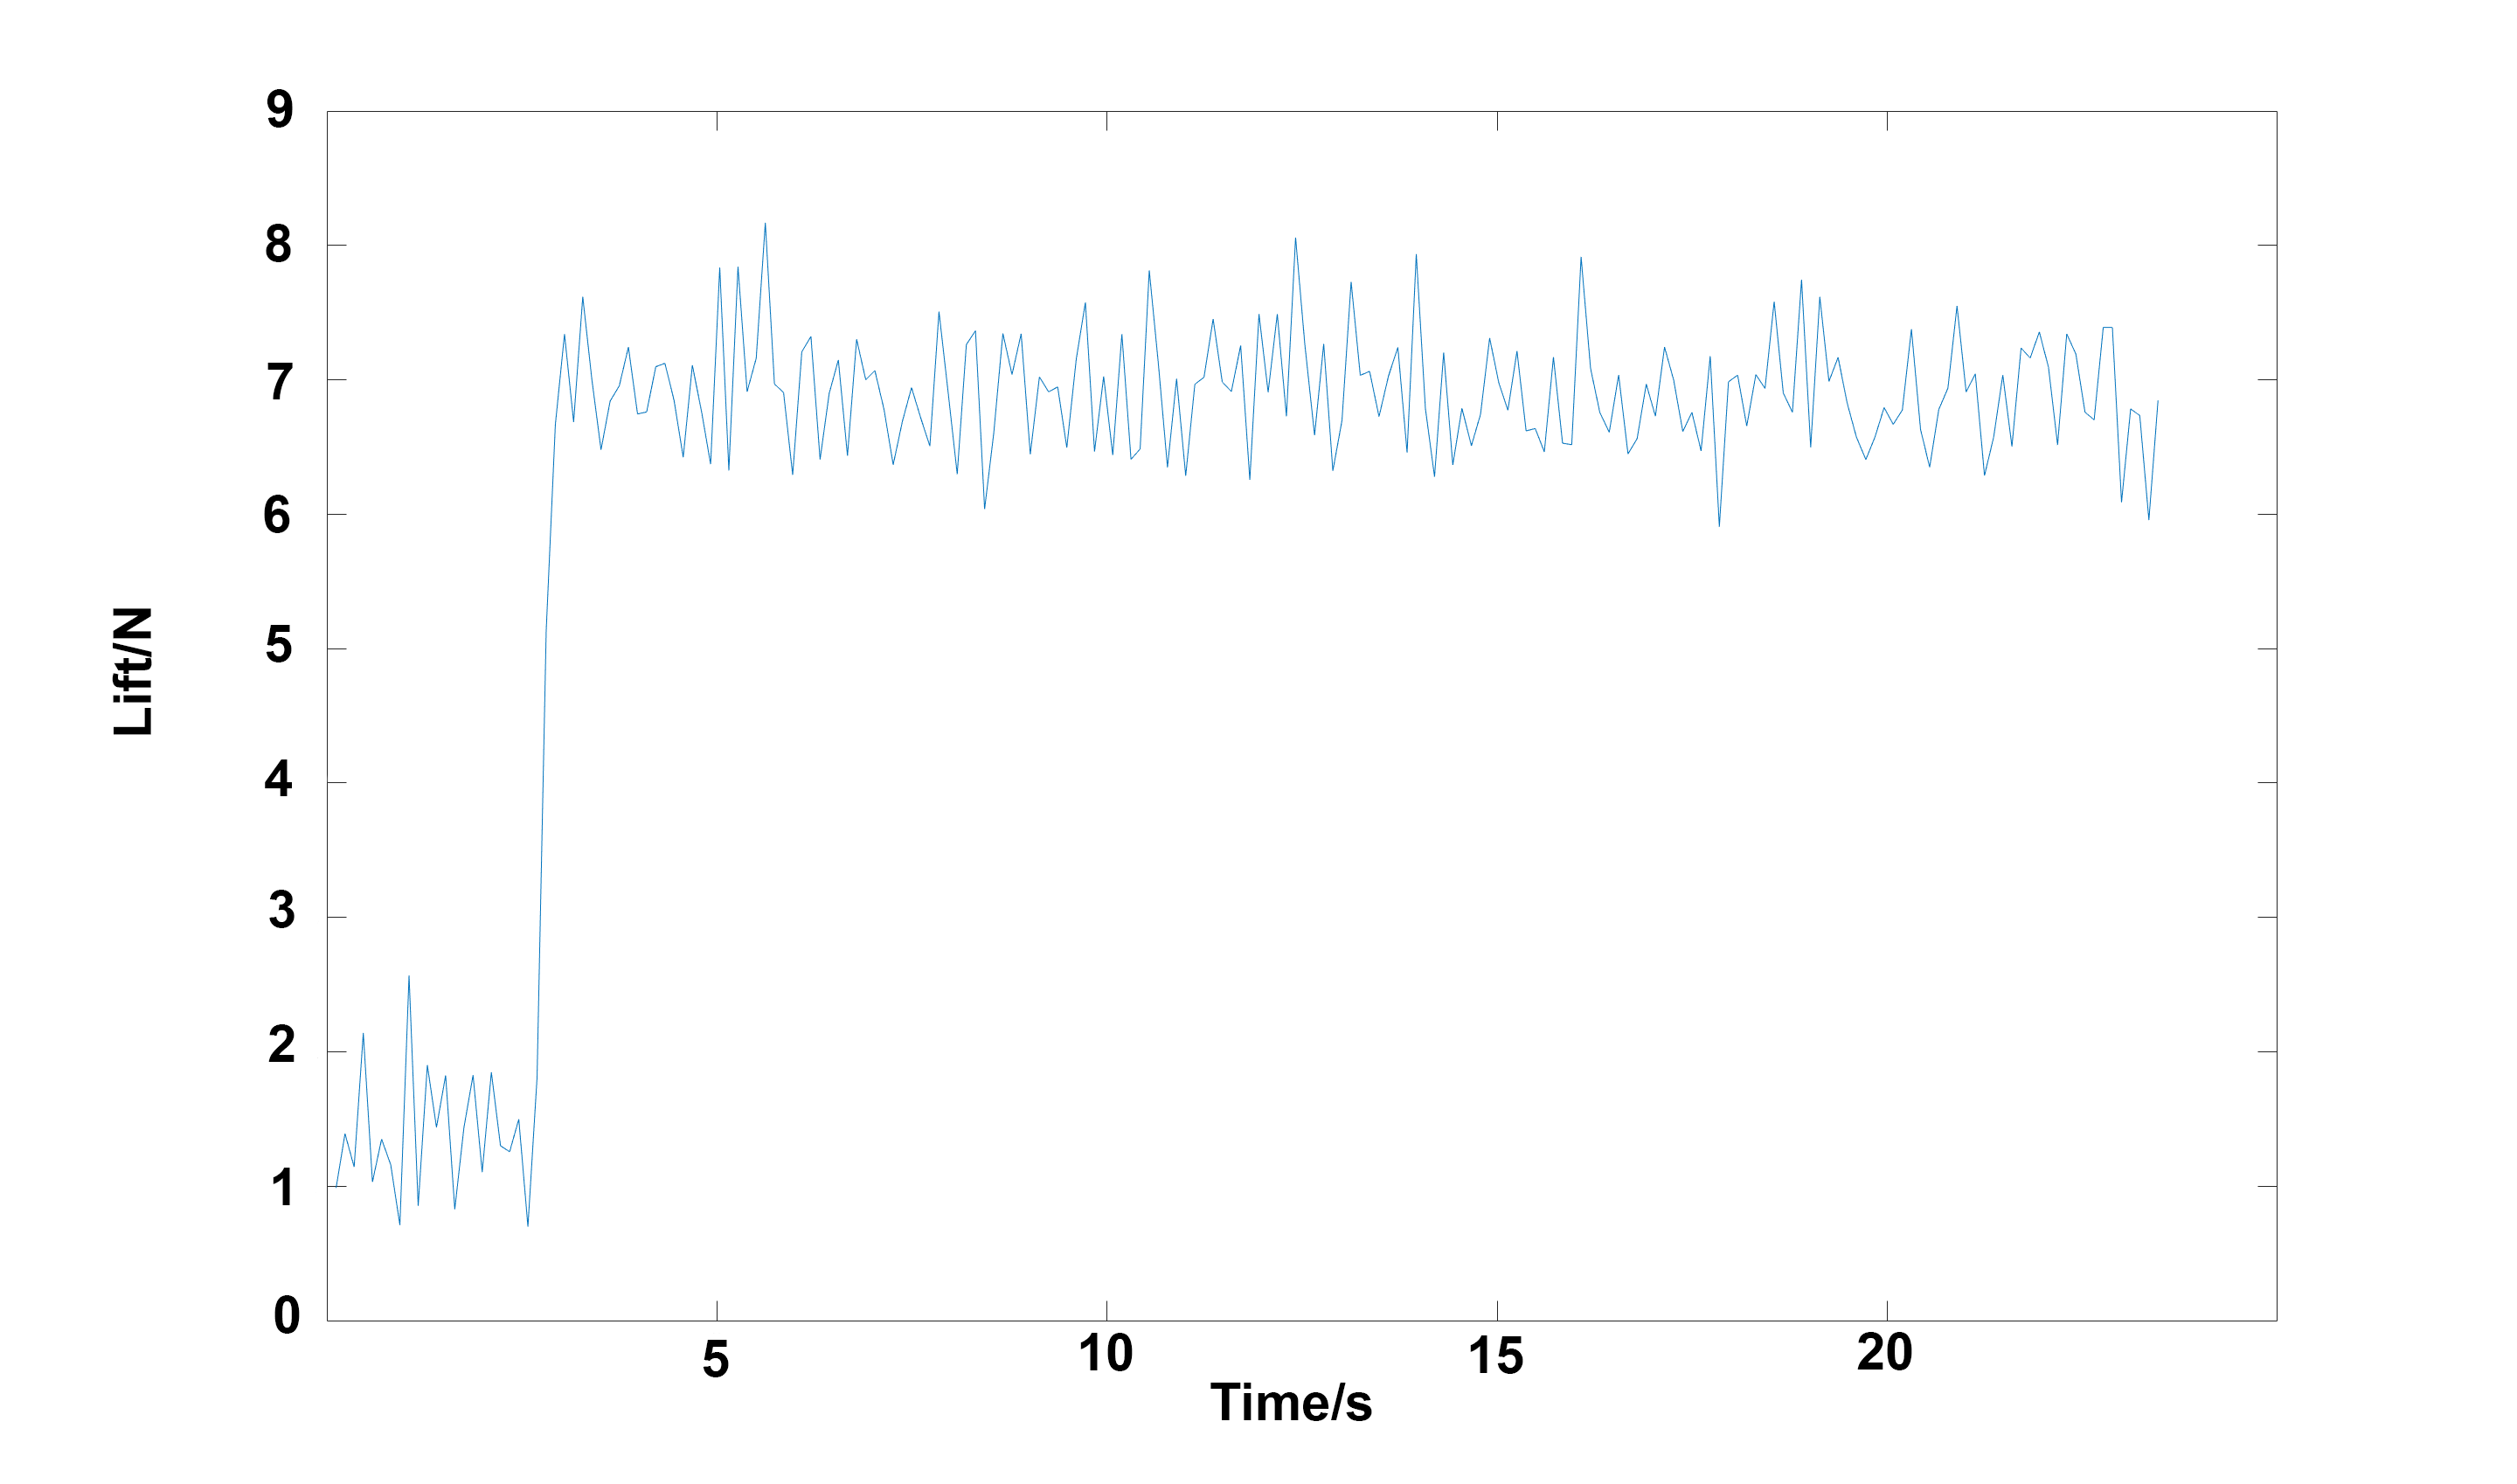
\includegraphics[width=1\textwidth,left]{fr.png}
\caption{Step response. The process variable (lift) changes as the flap moves from -60 deg to 60 deg.}
\centering
\end{figure}
The process begins by identifying when the step input was initiated($t_{0}$). From the data, is found that $t_{0}=2.577s$.

The half-way point $t_{2}$(when the lift is halfway between the initial value and the final value) and the time when 63.2$\%$ of the value between the initial and final lift occurs ($t_{3}$) is also found.  $t_{2}=2.771s$ and $t_{3} = 2.799s$.
The end of deadtime can be calculated ($t_{1}$). This is the time when the process variable (lift) starts rising. 
\begin{equation}
t_{1}=\frac{t_{2}-ln(2)t_{3}}{1-ln(2)}=2.708s
\end{equation}
$\tau$ is the time between the end of deadtime and the 63.2$\%$ point ($t_{3}$). 
\begin{equation}
\tau=t_{3}-t_{1}-0.091s
\end{equation}
$\tau_{del}$ is the duration between the step input initiation and the end of deadtime. 
\begin{equation}
\tau_{del}=t_{1}-t_{0}=0.13127s
\end{equation}
K is the ratio between the final and the initial value which is roughly 6/2=3. The last value needed to calculate the gains is $r$: 
\begin{equation}
r=\frac{\tau_{del}}{\tau}
\end{equation}
When all of the above parameters have been calculated, the gains can be calculated. 
\begin{equation}
K_{p}=\frac{1}{Kr}\left(\frac{4}{3}+\frac{r}{4}\right)=0.391
\end{equation}
\begin{equation}
t_{i}=\tau_{del}\frac{32+6r}{13+8r}
\end{equation}
\begin{equation}
K_{i}=\frac{K_{p}}{t_{i}}=1.7990
\end{equation}
\begin{equation}
t_{d}=\tau_{del}\frac{4}{11+2r}
\end{equation}
\begin{equation}
K_{d}=K_{p}t_{d}=0.0148
\end{equation}
\thispagestyle{fancy}
Using these values yielded a much improved result albeit not perfect.

\section{Airspeed Sweep test}
\thispagestyle{fancy}
\begin{figure}[H]
\centering
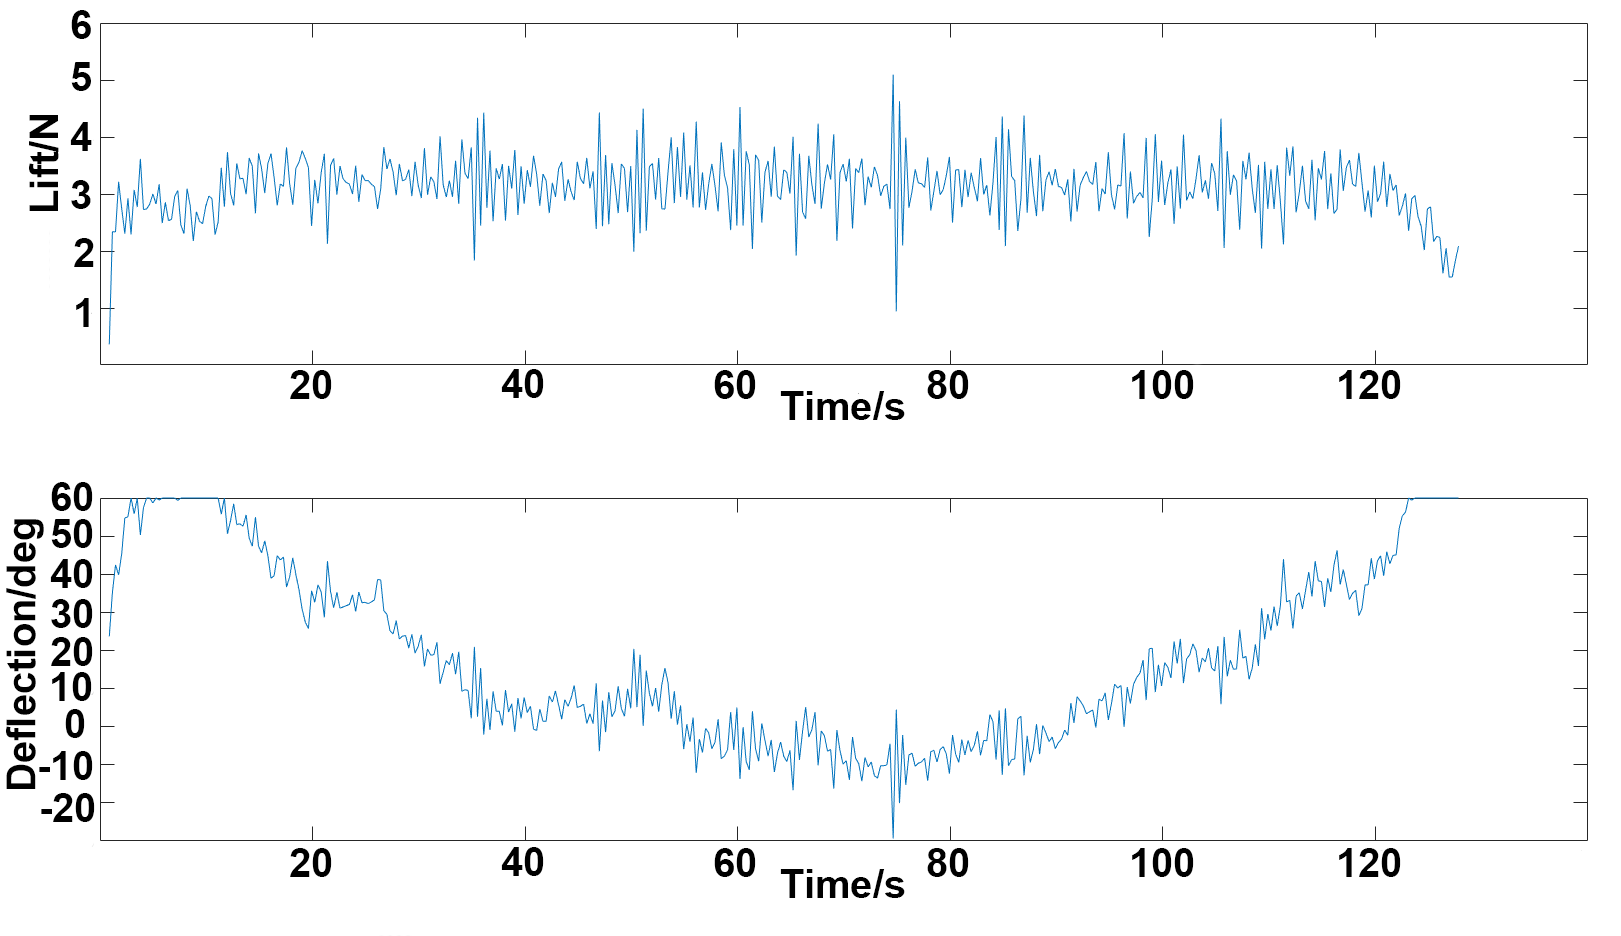
\includegraphics[width=1.1\textwidth,left]{sio.png}
\caption{Self-induced oscillations were noticed with the Cohen and Coon tuned controller. However, steady angles were also observed at steady conditions (around the 40s mark for instance).}
\centering
\end{figure}


This test was able to verify that the control system attempts to correct the lift when there is a change in airflow and is able to converge to a value when the conditions are held steady. By changing the airspeed in the wind tunnel, the controller should change the flap setting in order to maintain the lift. Eventually, a steady state flap angle should be observable. During high speeds, the flap should be at a relatively high angle to avoid excessive lift. Similarly at low speeds, the lift will be kept at the setpoint by a relatively low flap deflection angle. This test is different to gust tests because the airspeed changes more gradually than in a gust (which is characterised by an impulse in airspeed). 


Figure 7.4 shows the result from the airspeed sweep test. It shows that the controller is certainly responding to changing airspeeds and on averages holds the lift at 3.2N. Discrete sections are observable where the flap angle is roughly constant such as between 40s and 50s. During these times, the speed in the wind tunnel has stabilised at the setpoint. However, it is also inducing a few oscillations by itself. A major oscillation is visible at around 75s. This was again expected because the Cohen and Coon tuning method is used for fast response. This means that the controller is still a little too aggressive. 

The proportional gain had to be reduced to 0.02 to remove all self-induced oscillations. The integral and derivative gains were kept unchanged. 

The airspeed sweep test was repeated with the more robust controller and the results can be seen in figure 7.5 below.
\thispagestyle{fancy}
\begin{figure}[H]
\centering
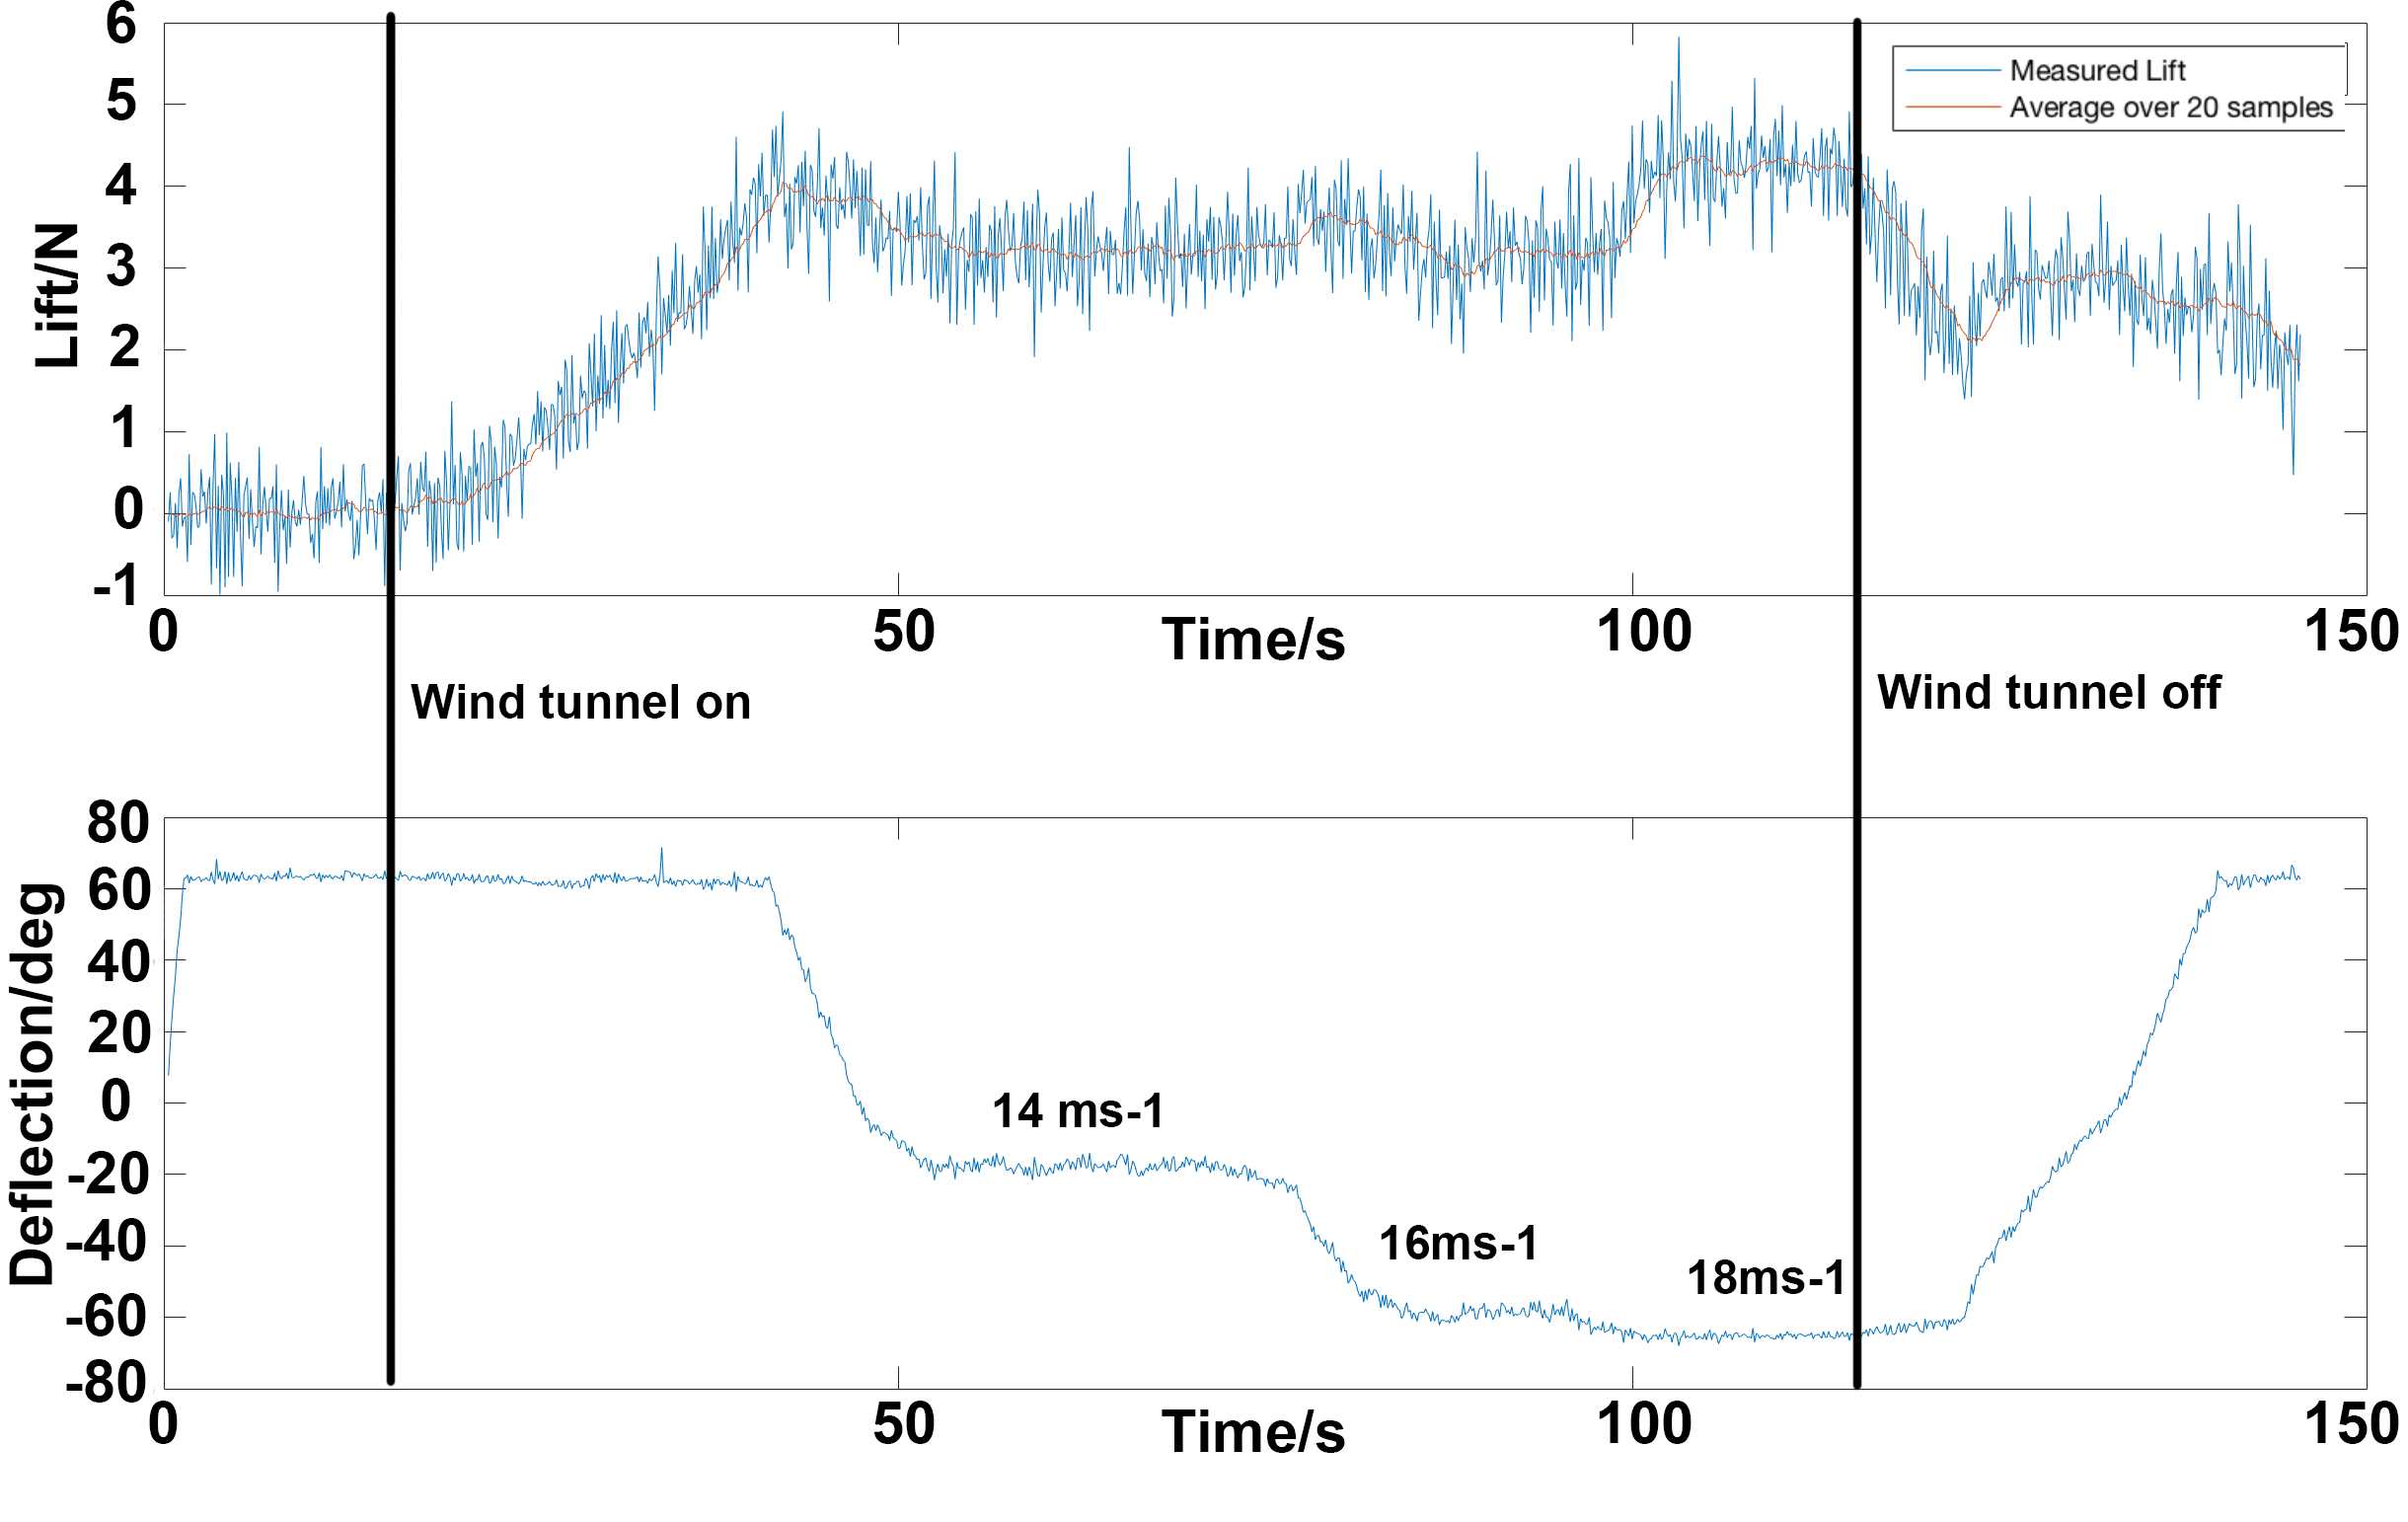
\includegraphics[width=1\textwidth,left]{sweep.png}
\caption{Airspeed sweep test. Note the steady states achieved by controller at different airspeeds with small overshoots. Compare this with the earlier iteration of the controller in figure 7.4}
\centering
\end{figure}

It can be seen that the controller is far less jittery than it was before in figure 7.4. It also clearly shows the controller's ability to converge to a certain value. The lift is held steady at 14 meters per second airspeed when the flap is at roughly -20 degrees (seen between 50s and 70s). As the wind tunnel airspeed ramps up, it can be seen the controller manages to keep the lift fairly constant. The only exception is when the system is saturated. This is seen when the wind tunnel is off or ramping up to $14ms^{-1}$ (between 0s and 40s). The flap is fully down while the speed is not high enough to produce the setpoint lift. The opposite situation is also observed. At $18ms^{-1}$ (between 100s and 120s), the speed is too high. Even when the flap is saturated at $-60^{\circ}$, the lift cannot be reduced to the setpoint. 

The test shows that the control system works very well in steady conditions as long as the actuator is not saturated. 

\section{Gust Response}
\thispagestyle{fancy}
\begin{figure}[H]
\centering
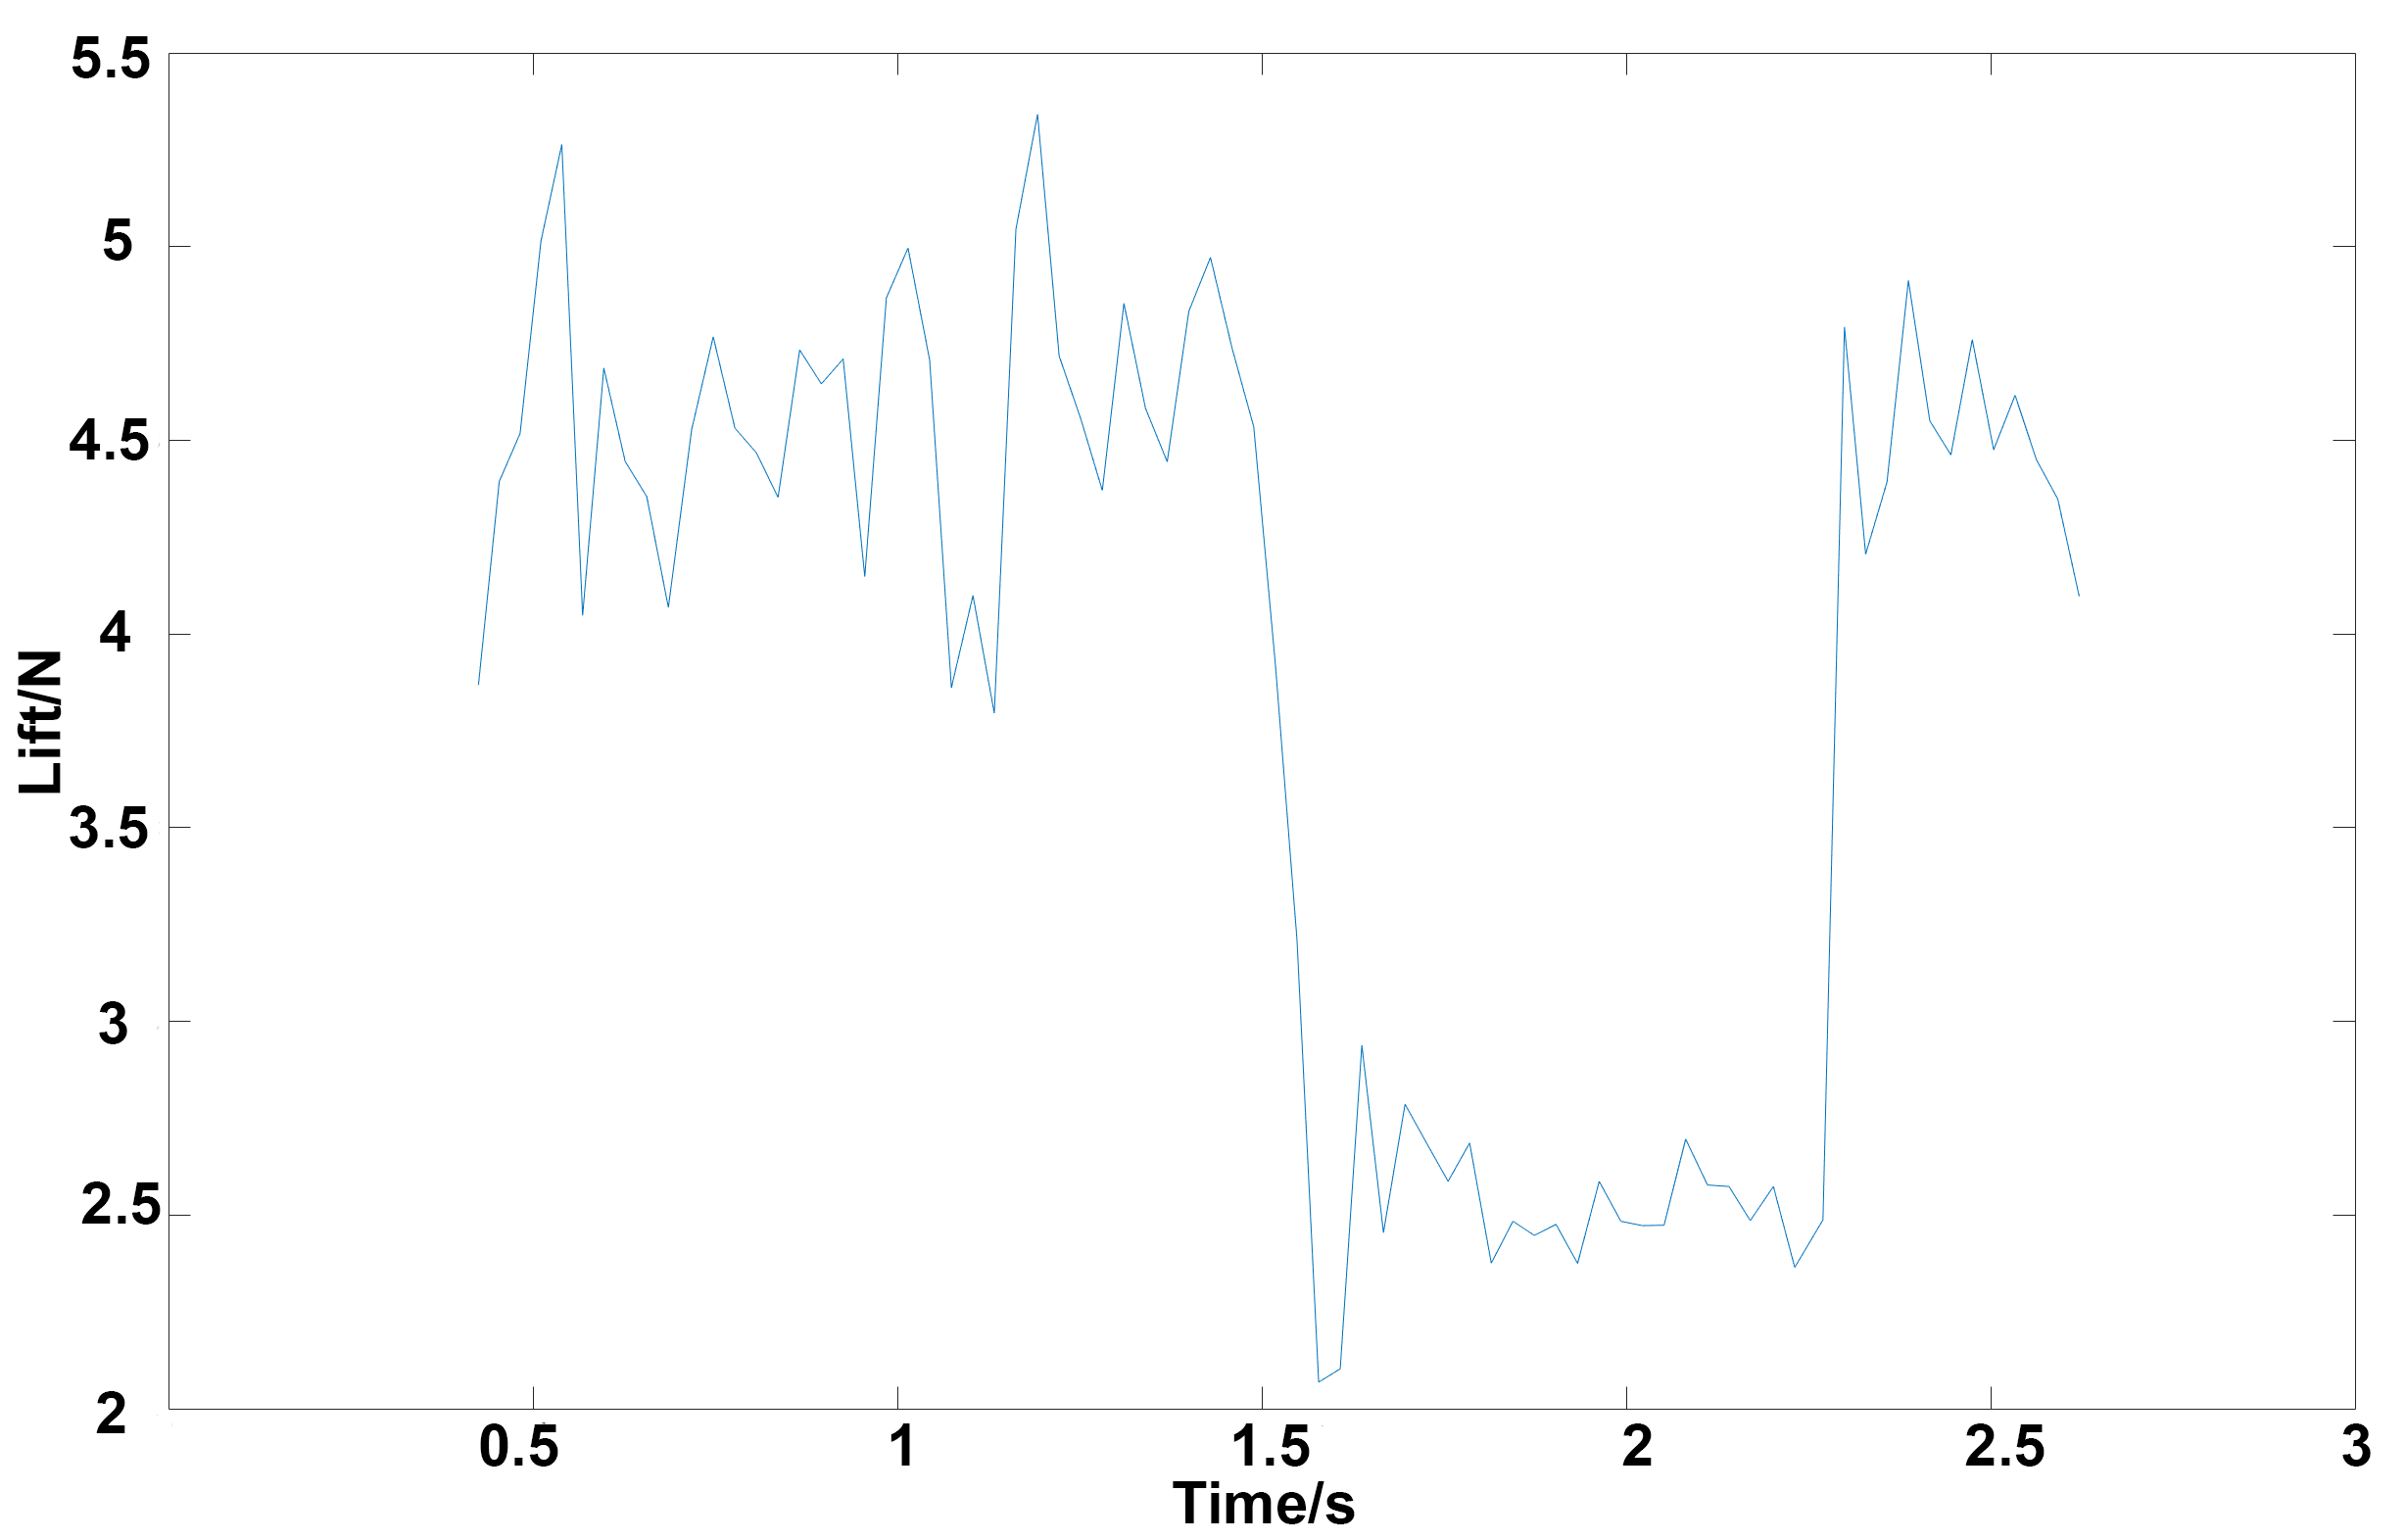
\includegraphics[width=1\textwidth,left]{grnc.png}
\caption{Impulse in lift as a result of the gust. Note the nominal lift is at 4.6N. This agrees with Xfoil.}
\end{figure}
The airspeed sweep test confirmed that the control system works in normal conditions. In this test, the controller will be tested through an impulse. The gust generator will be used to produce a large and a short lived drop in airspeed and the lift. To achieve this, the gust flaps were held steady at 10 degrees angle of attack towards each other. Then the flaps were suddenly deflected away from each other at 30 degrees. This caused a drop in airspeed and the lift. 
\newline
\newline
To get an idea of how well the system performs, the lift through a gust was measured with the controller disabled. A definitive drop in lift was observed.   
\newline
\newline
\thispagestyle{fancy} 
Figure 7.6 above shows the lift on the wing changes through a gust when the controller is disabled and the trailing edge flap is set to 0 degrees. As a side note, this test also shows that the lift estimator corroborates with Xfoil predictions (see Appendix C). 
\newline
\newline
\newpage
The controller was enabled and the same test was repeated. Figure 7.7 below shows the graph of the test. 
\newline
\newline
\thispagestyle{fancy}
The gust was initiated at roughly 27.5s and is clearly visible as a great drop in lift. This is counteracted by the controller's attempt to increase lift by increasing the flap deflection angle by over 30 degrees. The lift production returns very quickly to the original value which confirms that the control system works well. The lift crosses 3.2N roughly 0.2s after the gust but it is difficult to identify the settling time because of the noisy data. However, the relatively quick recovery of the loss of lift makes this project a resounding success. 
\begin{figure}[H]
\centering
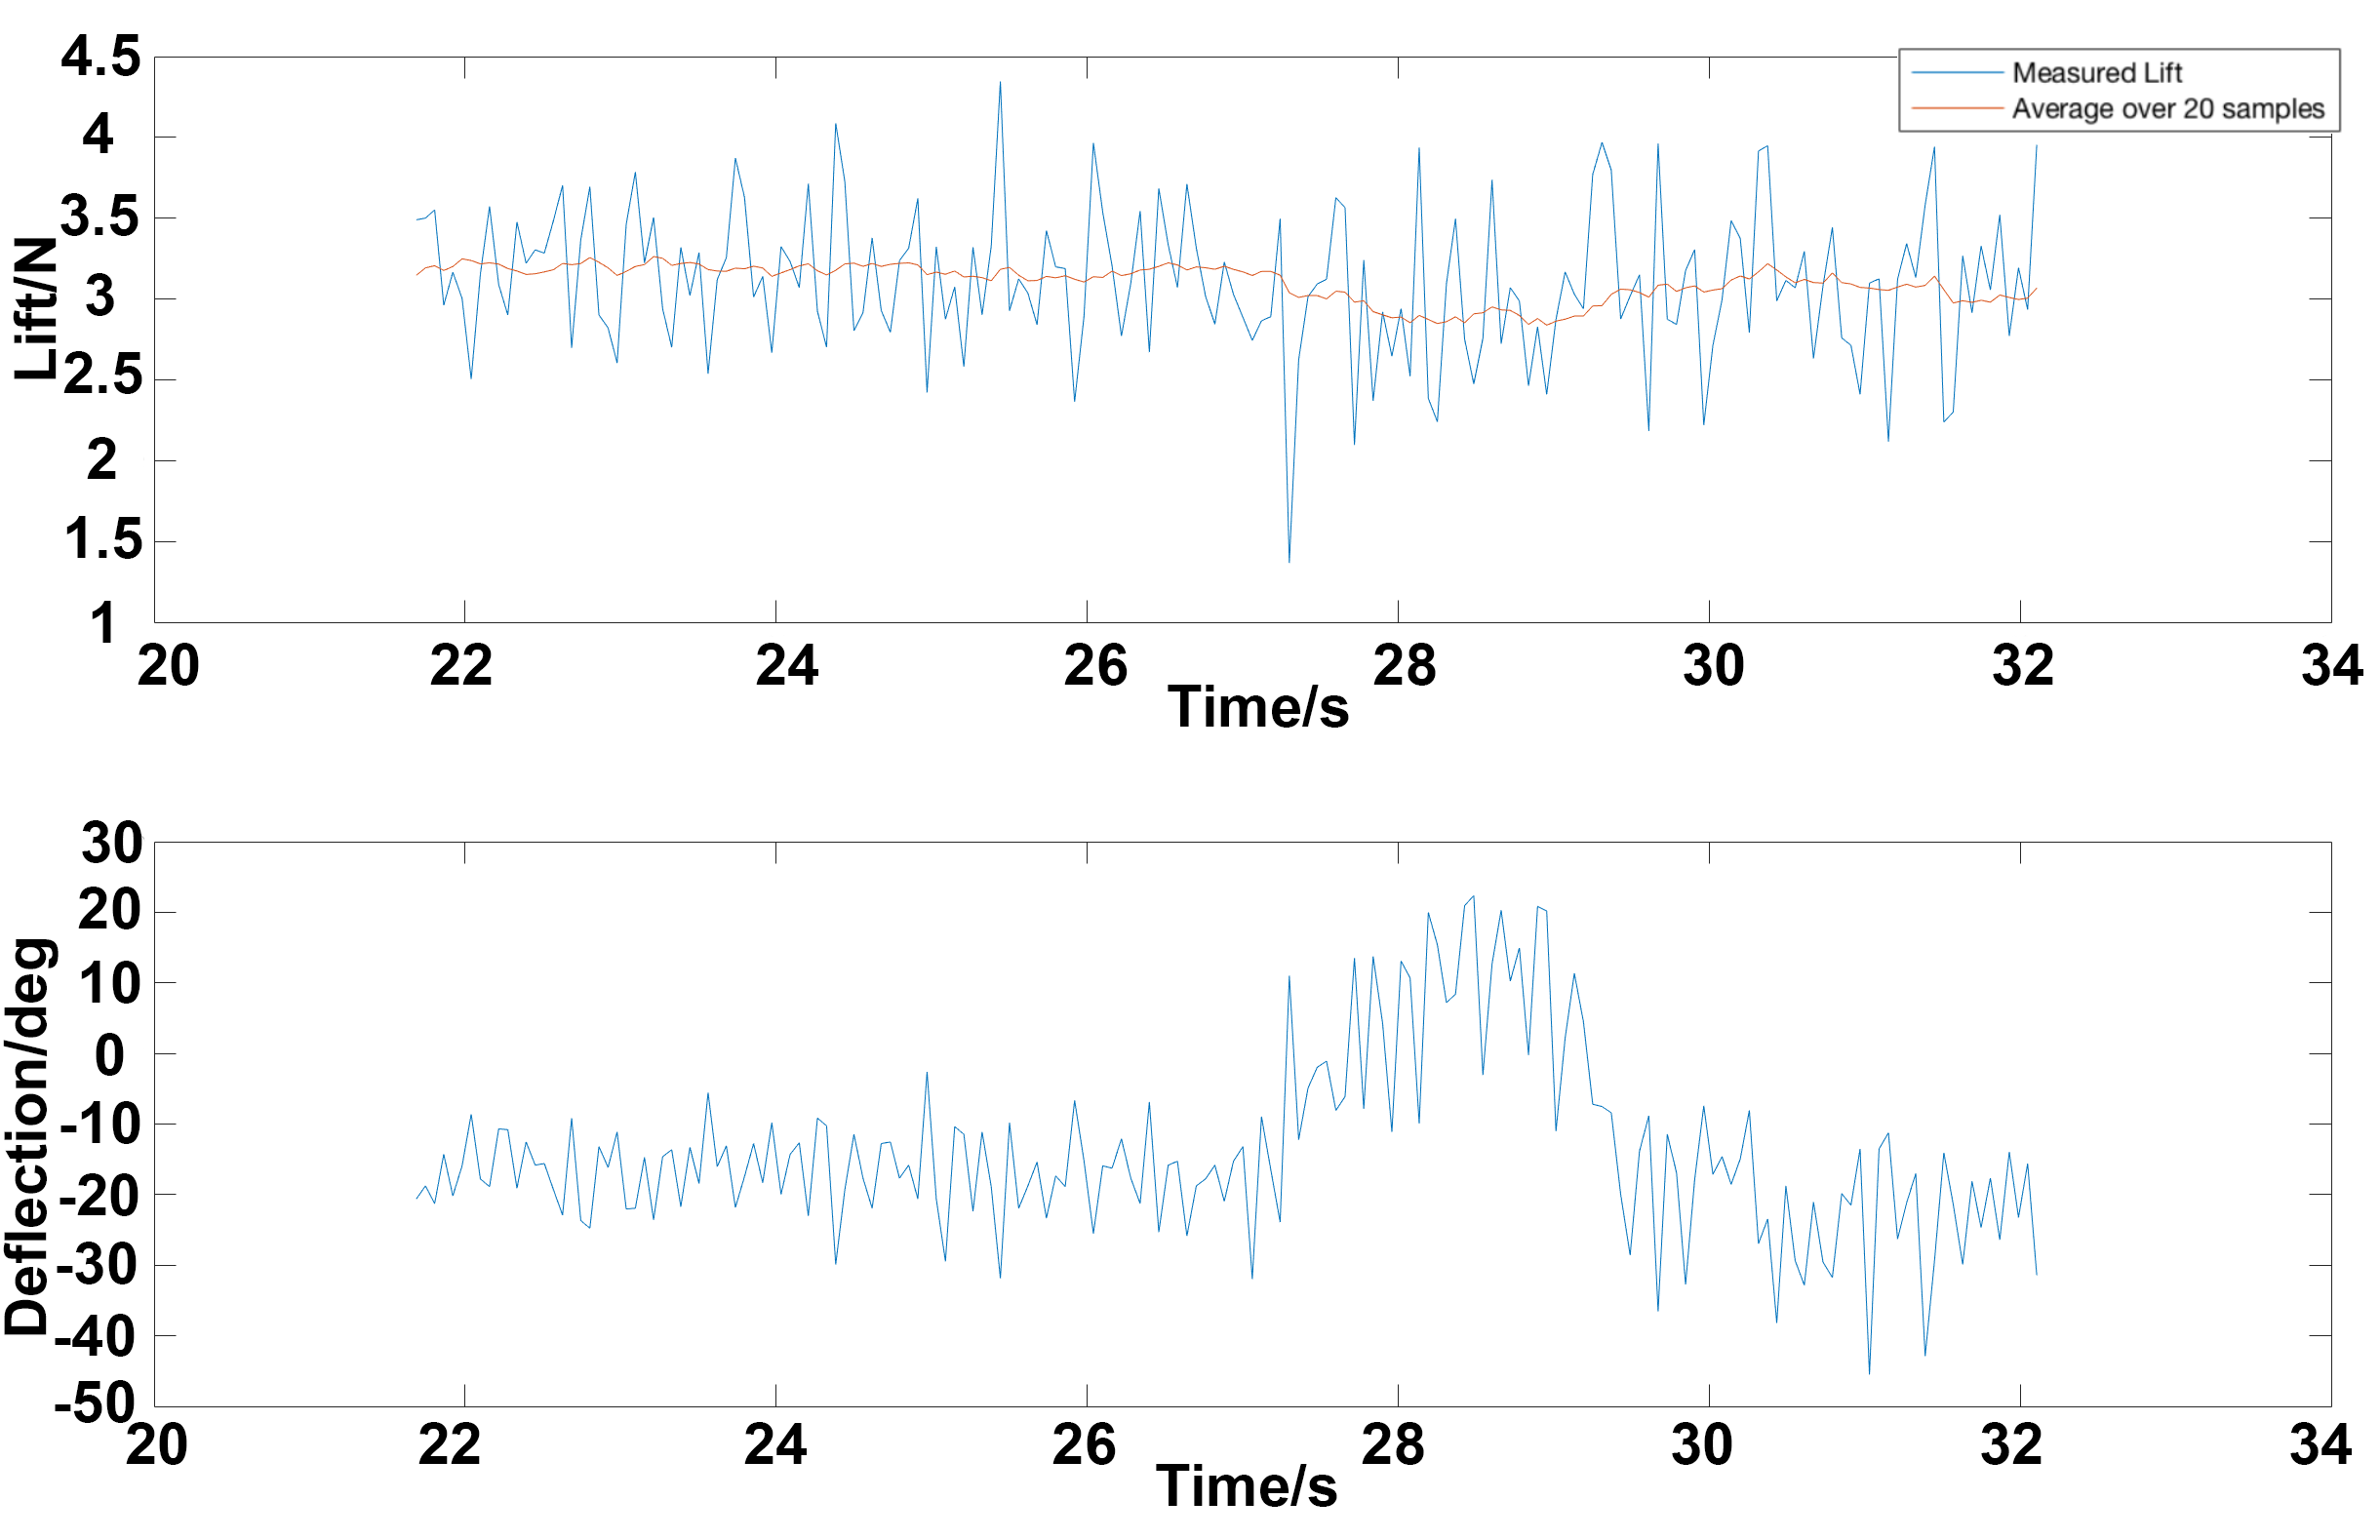
\includegraphics[width=1\textwidth,left]{gr.png}
\caption{Lift and flap angle vs time. Note the big drop in lift and the consequent increase in flap angle in an attempt to recover the lost lift.}
\centering
\end{figure}
\newpage
\section{Discussion of results}
\thispagestyle{fancy}
This section compares the results obtained with the aims and objectives that were set out at the beginning of the project. 
\newline
\newline
First and foremost, the aim of the project was to design a control system than can suppress the rapid change in lift production seen by the wing through a gust. The study compared how the lift changed when the flap wasn't controlled to when it was controlled and the test confirms that this objective was fulfilled. The amplitude of the oscillation as well as the time within which the lift was returned to the nominal values was reduced. 
\newline
\newline
The system was also aimed to be good at holding the lift at steady state conditions. This objective was definitely met as shown by the airspeed sweep test. As the airspeed was changed, the flap settled at a new value but any deviation from the setpoint lift was negligible. 
\newline
\newline
Thirdly, a qualitative target was set. The settling time of the process variable should be about 0.13s. Although the exact settling time cannot be identified from the noisy data, the system crosses 3.2N for the first time 0.2s after the gust. Therefore, the settling time is definitely more than 0.13s. The control system is still more robust than what has been achieved by similar systems thus far. It was noticed that aggressively tuned controller will be very sensitive to noise. Specifically the derivative gain will react quite a lot to noise since the rate of change of the error will be quite high throughout. Therefore, this was always the smallest gain among the three.  
\newline
\newline
The amplitude of the oscillation on the wing should have been lower with controller present than without. With no control, the lift dropped from 4.5N to 2.5N which gives a $\Delta L$ of 2N. 
\newline
\newline
With control, the lift dropped from 3.2N to 1.5N. This gives a $\Delta L$ of 1.7N. In this regard, the controller did slightly better. 
\newline
\newline
With all the tests it can also be assumed that in a positive gust, the controller will behave similarly because lift change is roughly linear with flap deflection (see section 5.3). Positive gusts were created in the wind tunnel by the flaps deflecting inwards. However, the lift became a lot more noisier and the controller found it impossible to control it. It was believed to be the effect of a turbulent wake from the gust generator which the wing would be in the middle of.  
\newline
\newline
The last aim was to design the control system from first principles and then validate it during testing. It is quite clear that the model is flawed because the estimated PID gains and manually tuned PID gains are vastly different. But the reasons why the Simulink model did not work are also quite clear and discussed in the further recommendations chapter. So the study can give advice on how to get a better approximation of the plant. 
\newpage
\chapter{Conclusion}
A new approach to control the flight trajectory was investigated in this study with an emphasis on gusts and short period oscillations. Using pressure sensors to control lift was theoretically proven to have several benefits over simply correcting the flight attitude. 
\newline
\newline
A simulation model was made to get first estimates for controller parameters. Consequently, the controller was tested in a wind tunnel. 
\newline
\newline
The tests showed that the Simulink model can be improved and this will be discussed in the next section. Cohen and Coon tuning and manual adjustments improved the performance of the system. 
\newline
\newline
The tuned controller performed very well in gradually changing airspeeds as shown in the airspeed sweep test. 
\newline
\newline
It also performed very well in gusts. This can be useful for mitigating short period oscillations or gusts in general.   
\section{Further recommendations}
\thispagestyle{fancy} 
The successful outcome of this project shows that it might be worthwhile to carry out further work in order to implement this on a real flight and test the controller through a real SPO. 
\newline
\newline
After completing this project, it is clear to me that several things can be done in the future to obtain a faster and more robust system. 
\newline
\newline
Firstly, it's worth understanding why the self-induced oscillations occurred after Cohen and Coon tuning. The system is certainly stable because the oscillations do not increase and the controller always manages to remove them. Ideally, after a steady state is achieved there would be no reason for the controller action to oscillate. This phenomenon is most likely excited by the noise in the data. Reducing this noise can be effectively done by simply increasing the average window size. But this was not desirable because increasing the window size increases the loop time. According to Nyquist's theorem, the frequency of the loop should be at least twice than the oscillation's frequency. But by experimentation it was seen that in practice the loop time has to be many times faster than this so that the system actually responds to disturbance. 
\newpage
The window had to be reduced to 20 samples to make the system responsive enough.  
\newline
\newline
A severe bottleneck was caused by the relatively slow I2C bus. In the future, it will certainly be beneficial to invest in faster sensors such as the ones based on the SPI bus. This will allow averaging over more samples reducing the noise. 
\newline
\newline
\thispagestyle{fancy} 
Alternatively, advanced filters such as a Kalman filter should be strongly considered. A problem with the Kalman filter is that it is difficult to determine the tuning parameters.  \cite{kf1} Some fairly advanced systems have been developed to calculate these parameters such as "reinforcement learning"\cite{kf2} which involved some trial and error and dynamic programming in order to optimise the filer. 
\newline
\newline
The Simulink model that was made had a few flaws that may have given an inaccurate representation of the system. 
\newline
\newline
\thispagestyle{fancy} 
Adding white-noise to the Simulink model would ensure that the sensor noise is accounted for when calculating the PID gains. 
\newline
\newline
\thispagestyle{fancy} 
It was noticed that the servo throw was visibly reduced by 20-30 degrees when the flap was subjected to an aerodynamic torque in the wind tunnel. Clearly, the servo dynamics are different when a resistive torque is applied to it. This was not considered when approximating the servo dynamics in chapter 5. 
\newline
\newline
\thispagestyle{fancy}
Lastly, there were some minor concerns with the manufacturing quality of the laser cut parts. The surface of these parts were quite rough and could potentially cause turbulent flow. However these parts were either downstream of the pressure tappings or far away from them so the influence the surface roughness would have on the pressure readings is unlikely to amount to much.  
\thispagestyle{fancy}
\newline
\newline
On the whole, this study was a solid start to a new and unique application of control systems for flight trajectory control, and has brought to light what areas can be investigated next.   
\newpage

%----------------------------------------------------------------------------------------
%	BIBLIOGRAPHY
%----------------------------------------------------------------------------------------
\renewcommand{\bibname}{References}
\begin{thebibliography}{9}
\thispagestyle{fancy}
\addcontentsline{toc}{chapter}{References}
\bibitem{ama}
"Amazon Prime Air", Amazon.com, 2018. [Online]. Available:\url{ https://www.amazon.com/Amazon-Prime-Air/b?ie=UTF8&node=8037720011}. [Accessed: 22- Apr- 2018]. 
\bibitem{etkin}
B. Etkin and L. Reid, Dynamics of flight. Chichester: Wiley, 1996, pp. 15, 174,175.
\bibitem{huang}
C. Huang, Q. Shao, P. Jin, Z. Zhu and B. Zhang, "Pitch Attitude Controller Design and Simulation for a Small Unmanned Aerial Vehicle," 2009 International Conference on Intelligent Human-Machine Systems and Cybernetics, Hangzhou, Zhejiang, 2009, 
URL: \url{http://ieeexplore.ieee.org/stamp/stamp.jsp?tp=&arnumber=5336043&isnumber=5335881}
\bibitem{liu}
N. Li and M. Balas, "Aeroelastic Control of Wind Turbine Blade Using Trailing-Edge Flap", Wind Engineering, vol. 38, no. 5, p. 1, 2014.
\bibitem{lee}
J. Lee, J. Han, H. Shin and H. Bang, "Active load control of wind turbine blade section with trailing edge flap: Wind tunnel testing", Journal of Intelligent Material Systems and Structures, vol. 25, no. 18, pp. 2253-2255, 2014.
\bibitem{navion} 
R. Catterall  "State-Space Modeling of the Rigid-Body Dynamics of a Navion Airplane From Flight Data, Using Frequency-Domain Identification Techniques", 2003.
\bibitem{far}
"14 CFR 23.181 - Dynamic stability.", LII / Legal Information Institute, 2011. [Online]. Available: https://www.law.cornell.edu/cfr/text/14/23.181. [Accessed: 03- Feb- 2018].
\bibitem{chung} 
H. Chun and C. Chang, "Longitudinal stability and dynamic motions of a small passenger WIG craft", Ocean Engineering, vol. 29, no. 10, p. 1161, 2002.
\bibitem{short}
B. Aliyu, C. Osheku, P. Okeke, F. Opara and B. Okere, "Oscillation Analysis for Longitudinal Dynamics of a Fixed-Wing UAV Using PID Control Design", Advances in Research, vol. 5, no. 3, p. 6, 2015.
\bibitem{comp}
Python 3 vs C gcc (64-bit Ubuntu quad core) | Computer Language Benchmarks Game. [online] Available at: \url{https://benchmarksgame.alioth.debian.org/u64q/compare.php?lang=python3&lang2=gcc} [Accessed 13 Apr. 2018].
\bibitem{jd}
Anderson, Fundamentals of aerodynamics. New York: McGraw-Hill, 2011, p. 55.
\bibitem{shan}
C. Shannon, "Communication in the presence of noise", Proceedings of the IEEE, vol. 72, no. 9, p. 11, 1984.
\bibitem{gordon}
"Raspberry Pi | Wiring | Gordons Projects", Projects.drogon.net, 2018. [Online]. Available: \url{https://projects.drogon.net/raspberry-pi/wiringpi/}. [Accessed: 01- Feb- 2018].
\bibitem{cohen}
"Cohen Coon Tuning Method", Pages.mtu.edu, 2018. [Online]. Available: \url{http://pages.mtu.edu/~tbco/cm416/cctune.html}. [Accessed: 06- Apr- 2018].
\bibitem{kf1}
Saha, M., Goswami, B. and Ghosh, R. "Two novel metrics for determining the tuning parameters of the Kalman Filter". p.1, 2013.
\bibitem{kf2}
Goodall, C. and El-Sheimy, N. INTELLIGENT TUNING OF A KALMAN FILTER USING LOW-COST MEMS INERTIAL SENSORS. p.1, n.d.
\thispagestyle{fancy}

\thispagestyle{fancy}

\end{thebibliography}


%----------------------------------------------------------------------------------------
%----------------------------------------------------------------------------------------
%	THESIS CONTENT - APPENDICES
%----------------------------------------------------------------------------------------

\appendix % Cue to tell LaTeX that the following "chapters" are Appendices

% Include the appendices of the thesis as separate files from the Appendices folder
% Uncomment the lines as you write the Appendices

% Appendix A
\chapter{Manufacturing and assembly}

The main wing was split into four parts: the two ends of the wings, the middle section (as shown in figure 4.1) and the flap. Different manufacturing processes had to be utilised to obtain these parts quickly and of sufficient quality. 

\thispagestyle{fancy}
The middle section is geometrically complex due to the presence of the pressure tappings. It is not very practical to hand craft the part and not feasible through 2D processes such as laser cutting or foam cutting due to the 3D geometric features. 3D printing is the only process that is suitable and available for this component. Unfortunately, the span of the wing is too great (30cm) for the 3D printer so to ends of the wing need to be extended. The 3D printed part was made 20cm wide. 

To extend the wing by 5cm each side, the profile of the middle section was saved as a .dxf file. This profile was laser cut out of a 5mm thick plywood 20 times and glued together side-to-side. 

The flap was made similarly. The profile was laser cut 60 times and glued together. 

The main wing has been supported and mounted through two 6mm carbon fibre rods that go through the wing and attach to some fixtures on the walls of the tunnel. These fixtures were designed specifically for this project. 
\begin{figure}[H]
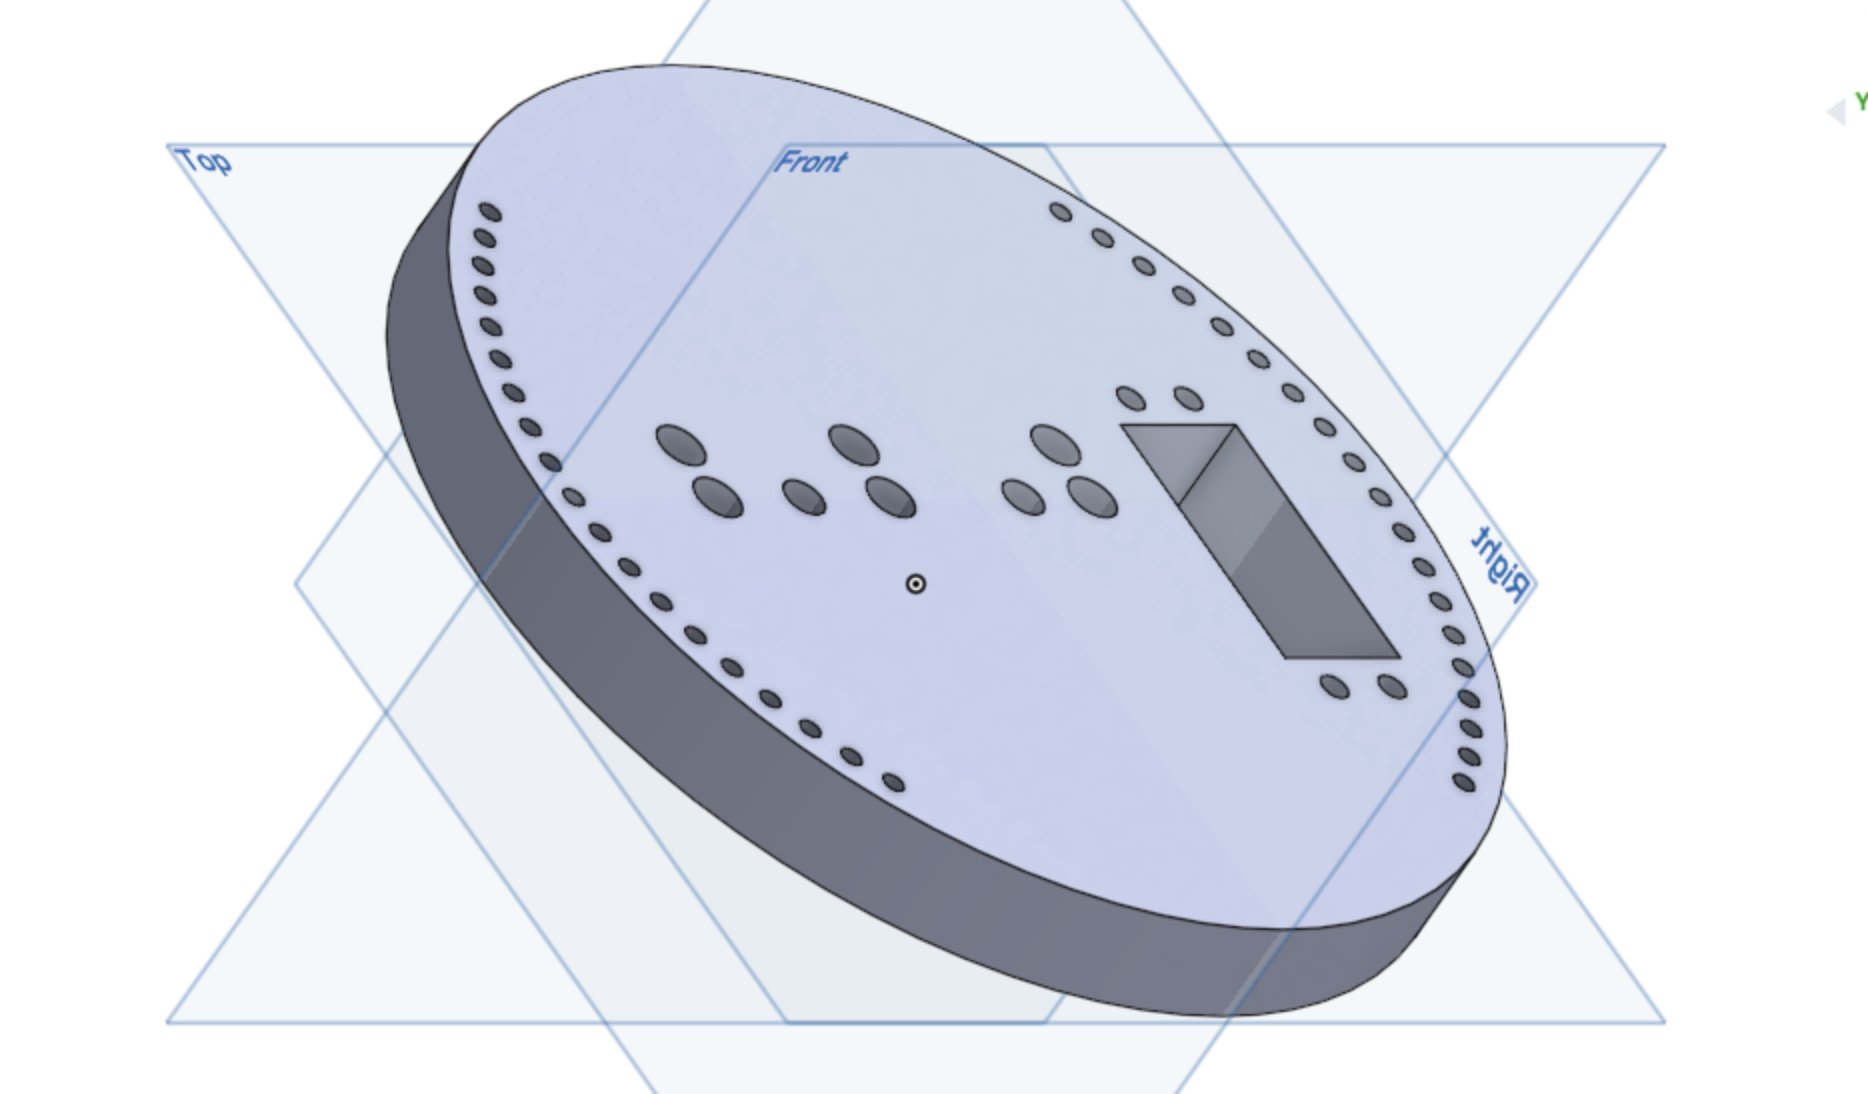
\includegraphics[scale=0.45]{fix.png}
\caption{Fixture on the right hand side of the wind tunnel}
\end{figure}
Looking upstream, the fixture disc on the right hand side (Figure 4.3) has holes for the carbon fibre rods, a cut out for the flap servo to be mounted in, six holes for the PVC tubes connecting the pressure tappings to the sensors and several holes near the edges to allow changing the angle of attack of the wing to a desired setting. The angular separation between these holes is 5$^{\circ}$. 
\thispagestyle{fancy}
\begin{figure}[h]
\centering
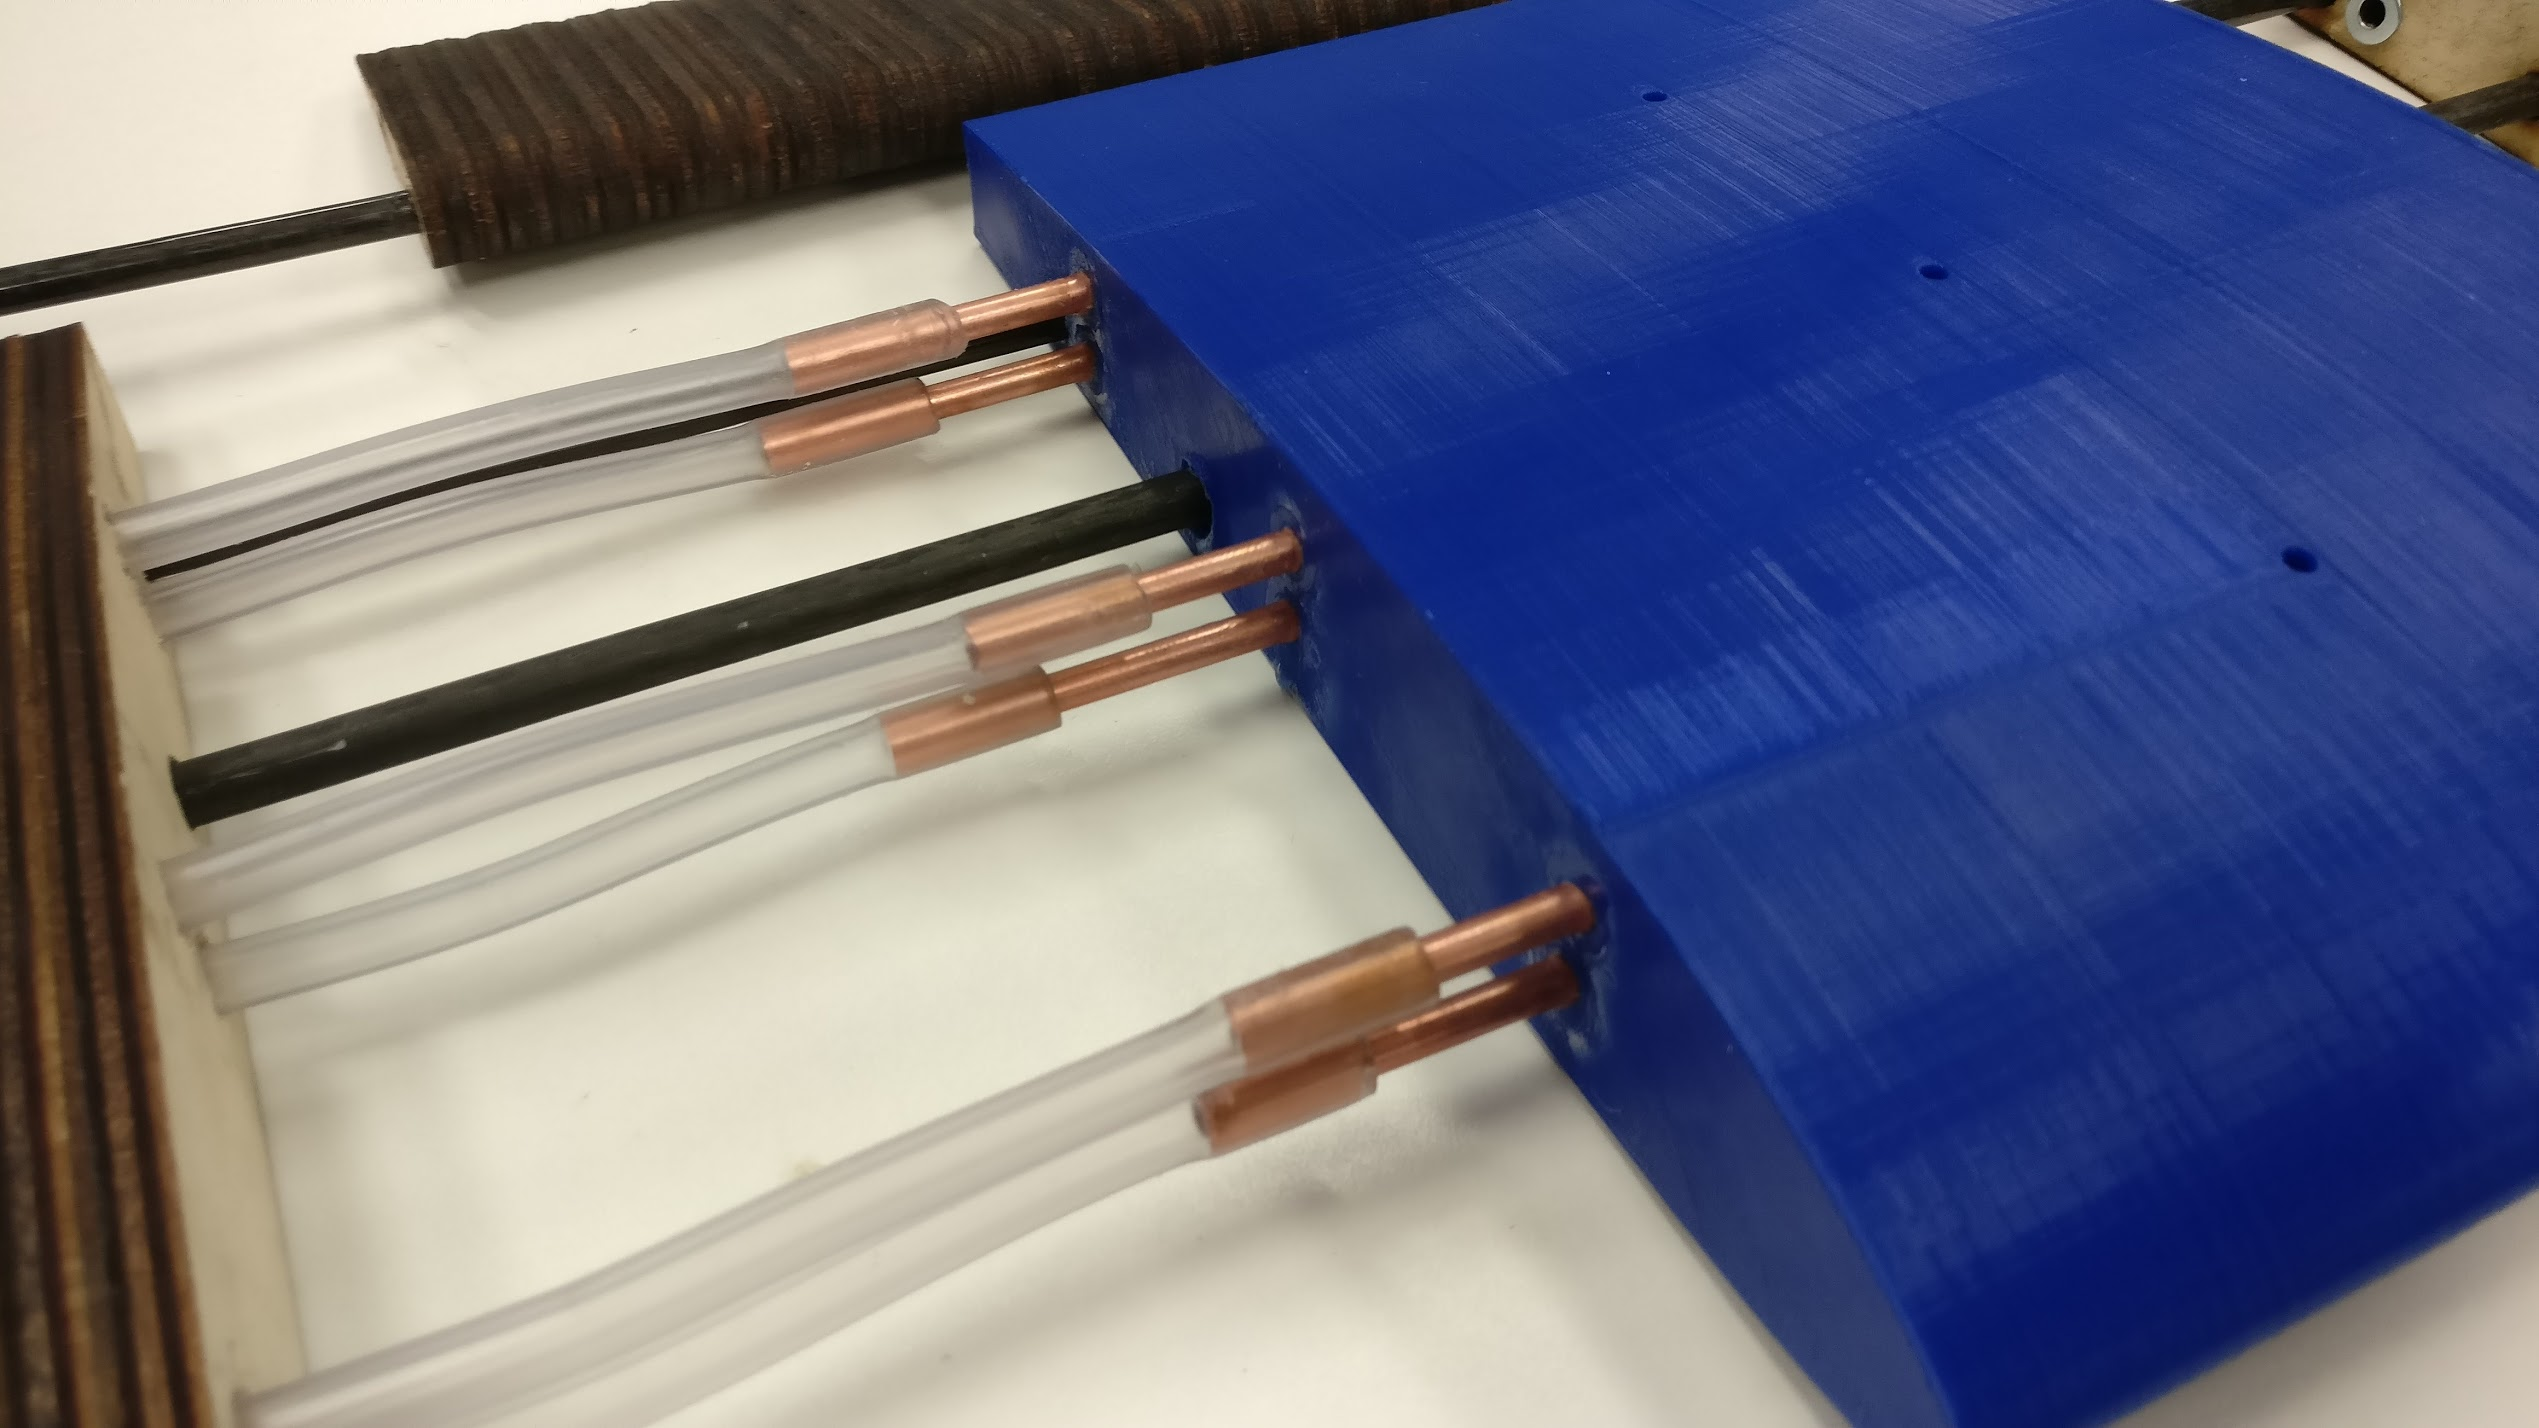
\includegraphics[scale=0.1]{pipe.jpg}
\caption{Picture of the PVC tubing and the midsection of the wing}
\centering
\end{figure}
The pressure tappings end at the right side of the middle section of the wing. Sections of a 4mm (outer diameter) copper pipe were placed in these holes and glued in place. \thispagestyle{fancy} These created "ports" which allowed easy and secure connection of the pressure tappings to the pressure sensors. Six equal sections of 3mm PVC tube(inner diameter) were cut to facilitate this connection. One end of each tube was secured to the pressure sensor ports, the other end had to be heated and expanded to fit onto the larger copper ports on the wing. This provided an excellent tight seal which is beneficial because less pressure will be lost. 
\thispagestyle{fancy}

\thispagestyle{fancy}
\newpage
\begin{figure}[H]
\centering
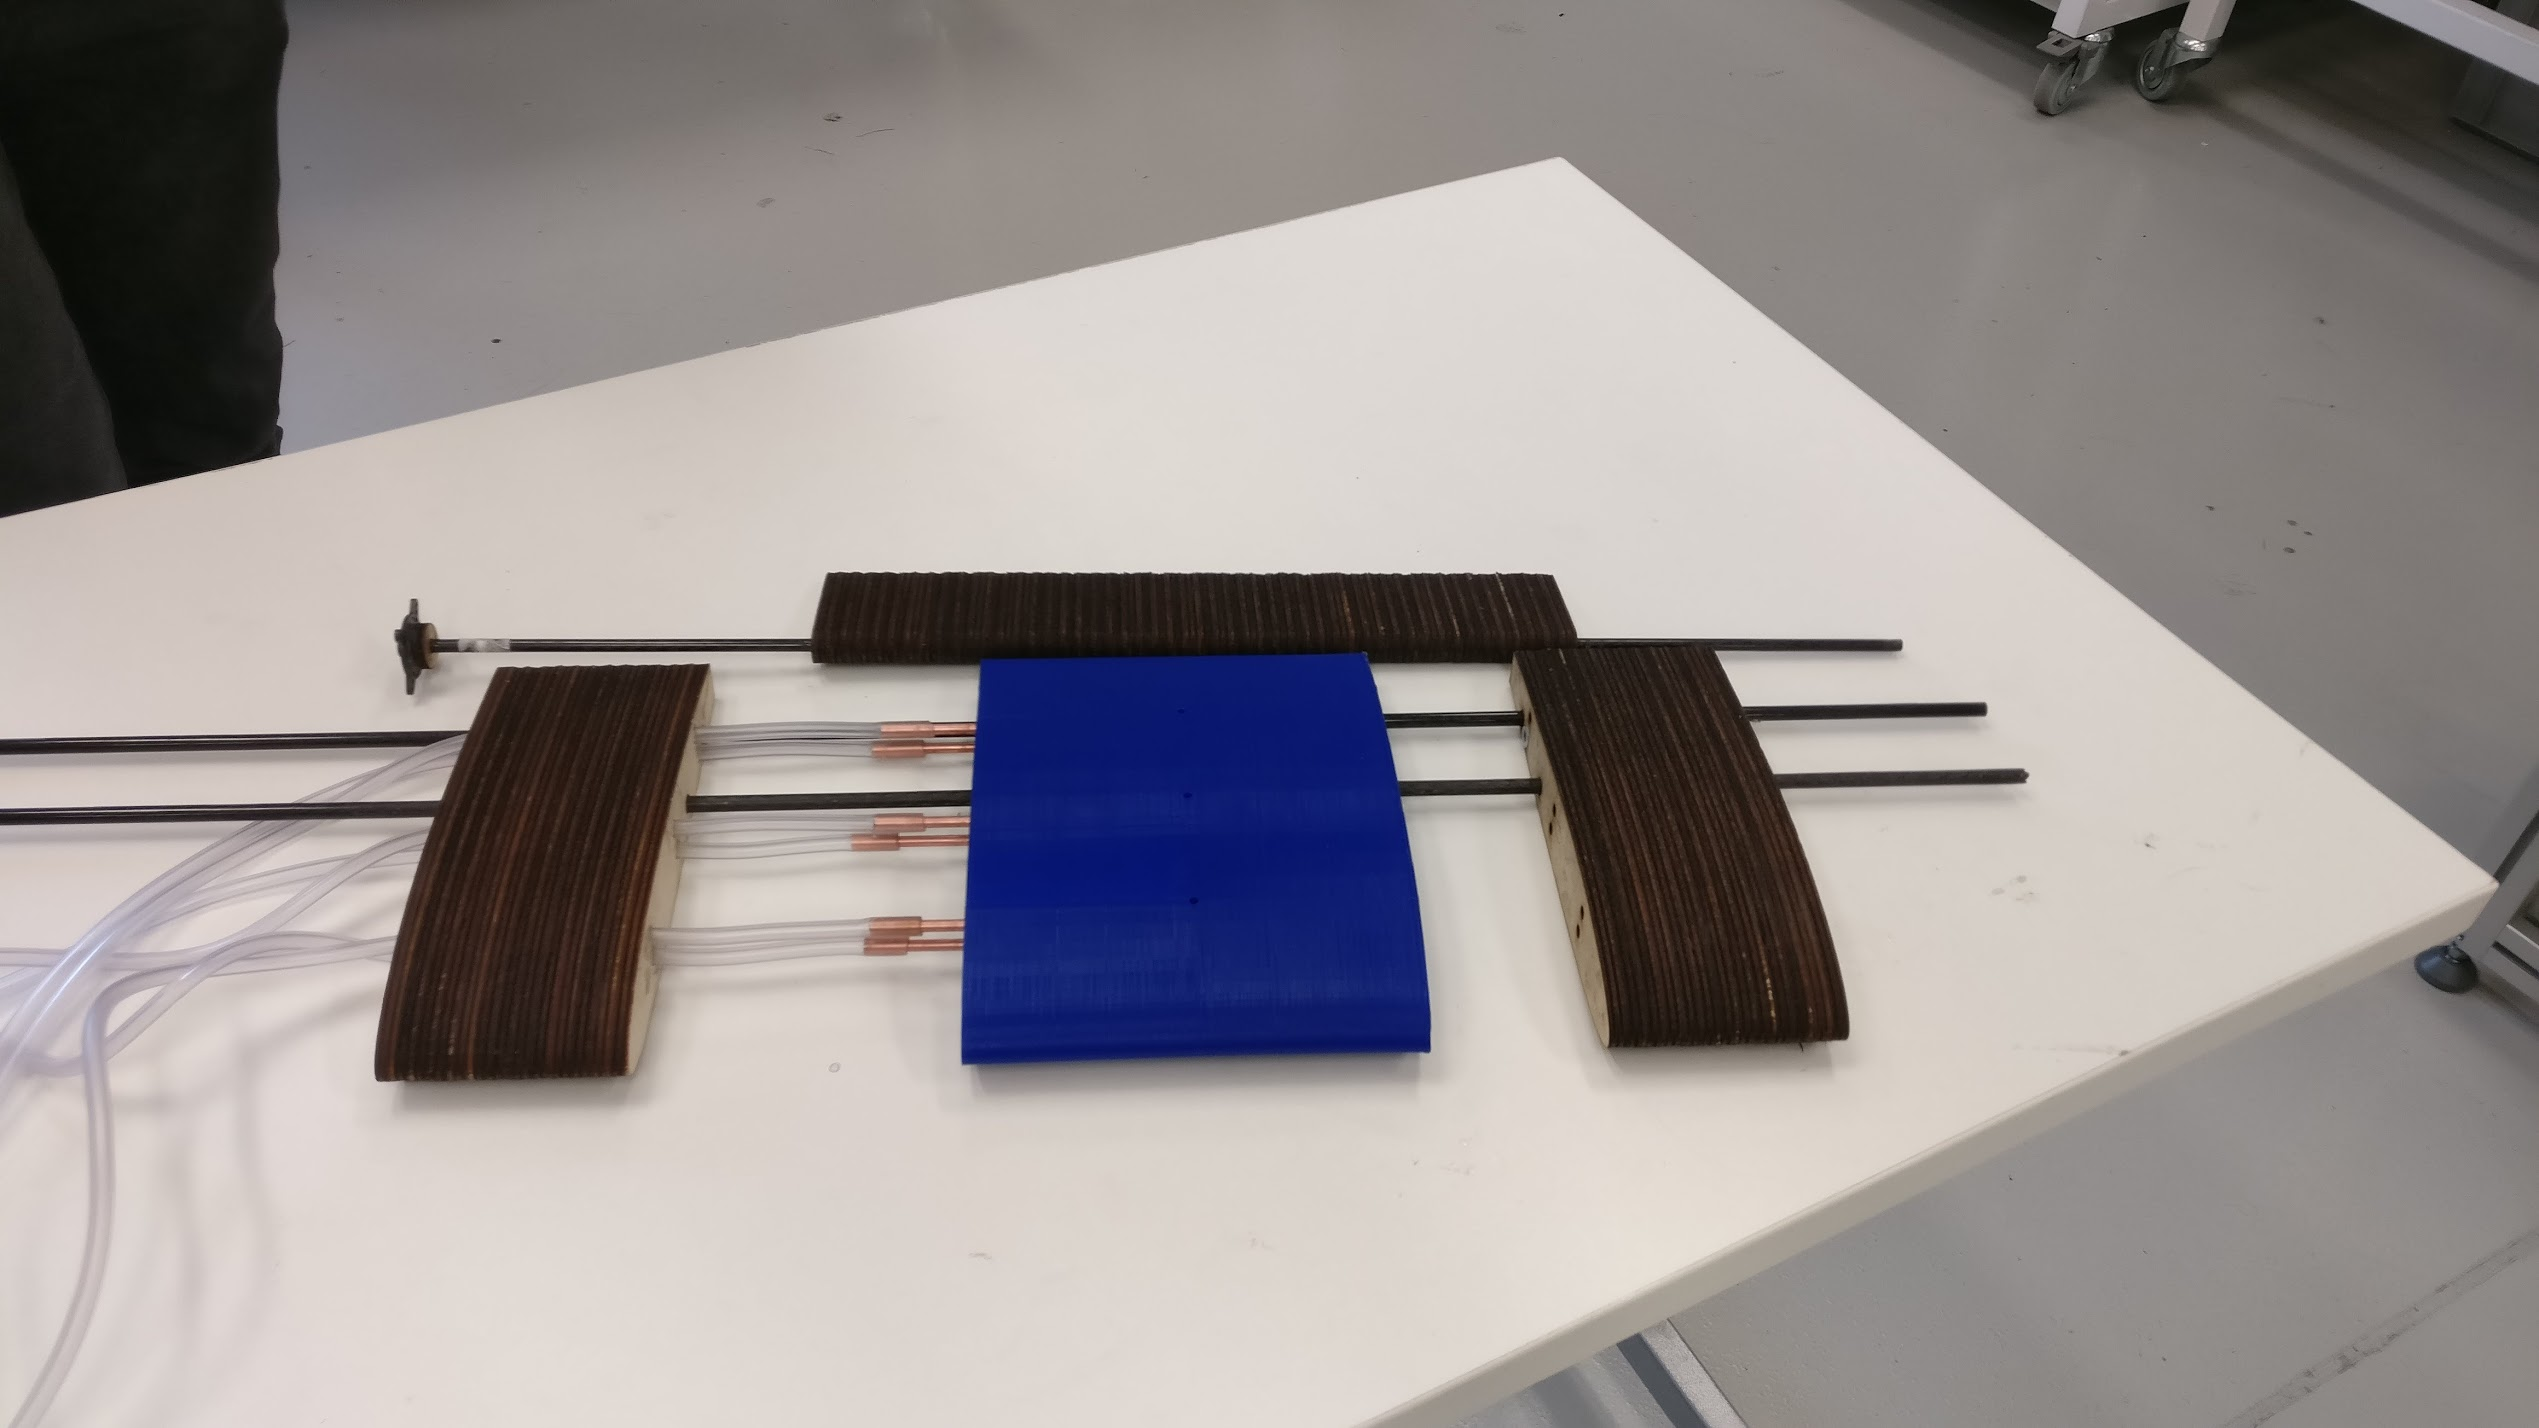
\includegraphics[scale=0.12]{integ.jpg}
\caption{Picture showing how the different parts of the wing were integrated}
\centering
\end{figure}
\begin{figure}[H]
\centering
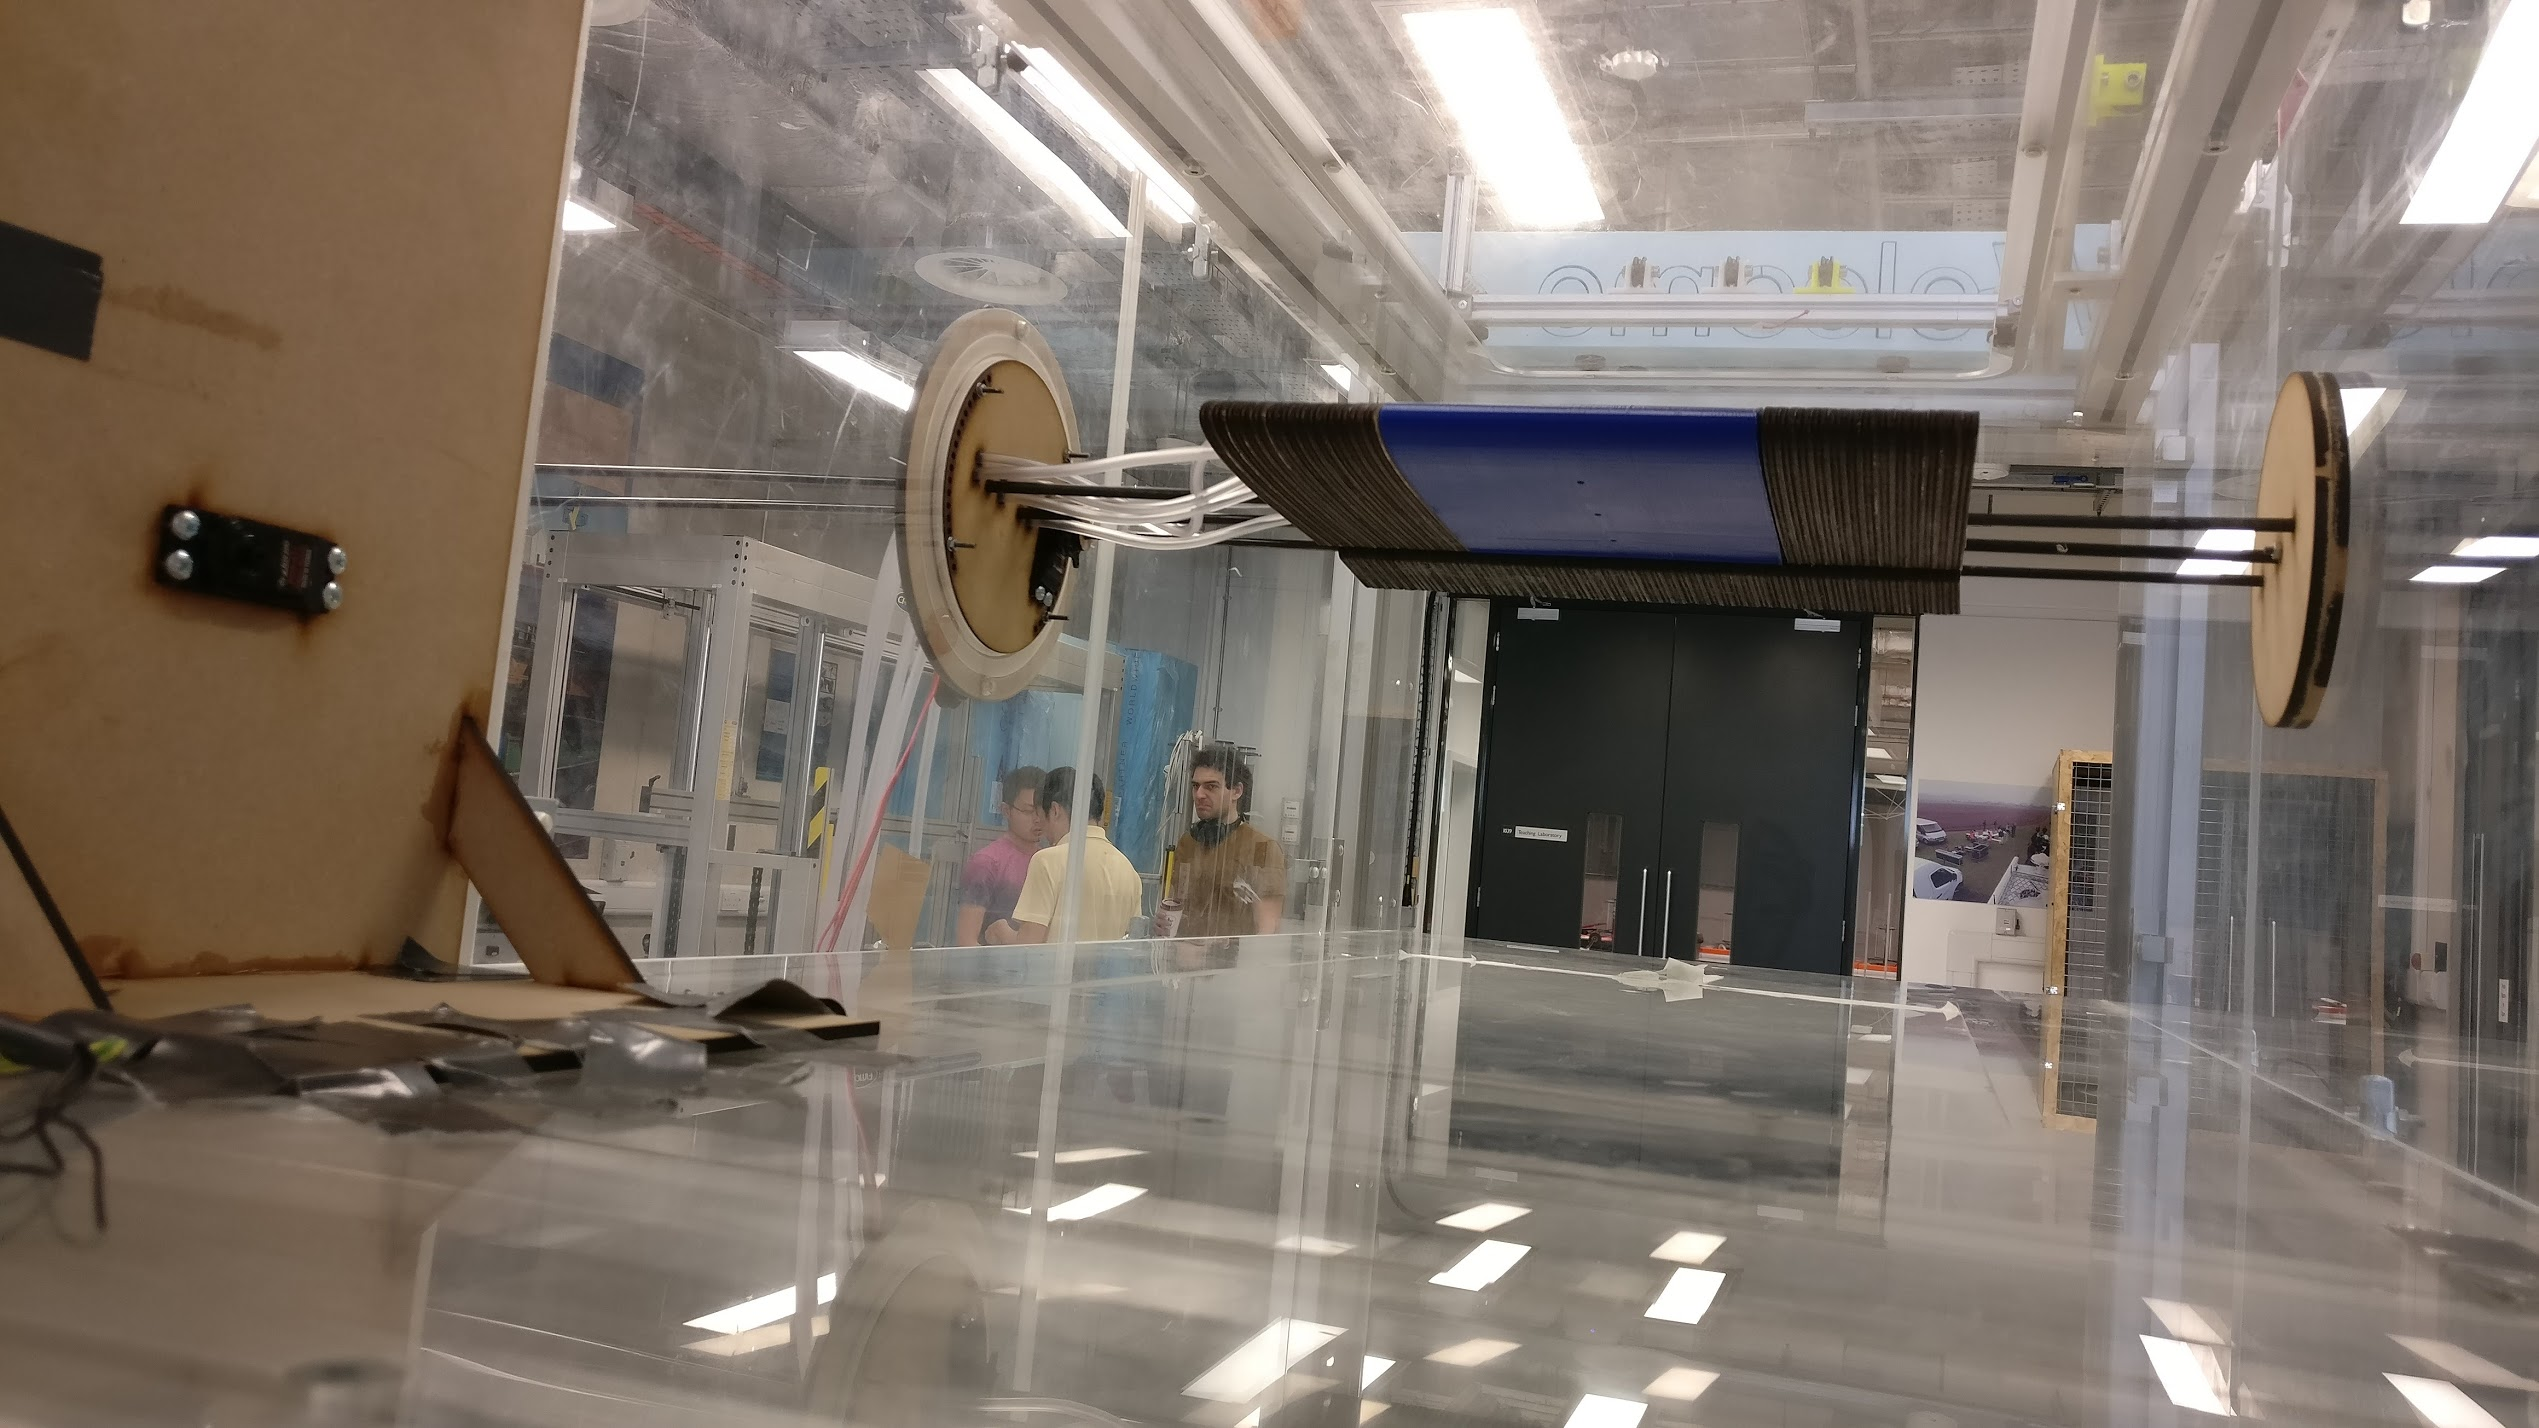
\includegraphics[scale=0.15]{wind.jpg}
\caption{Picture showing the main wing assembly in the wind tunnel}
\centering
\end{figure}

\chapter{Risk Assessment} % Main appendix title
\thispagestyle{fancy}
\begin{figure}[H]
\centering
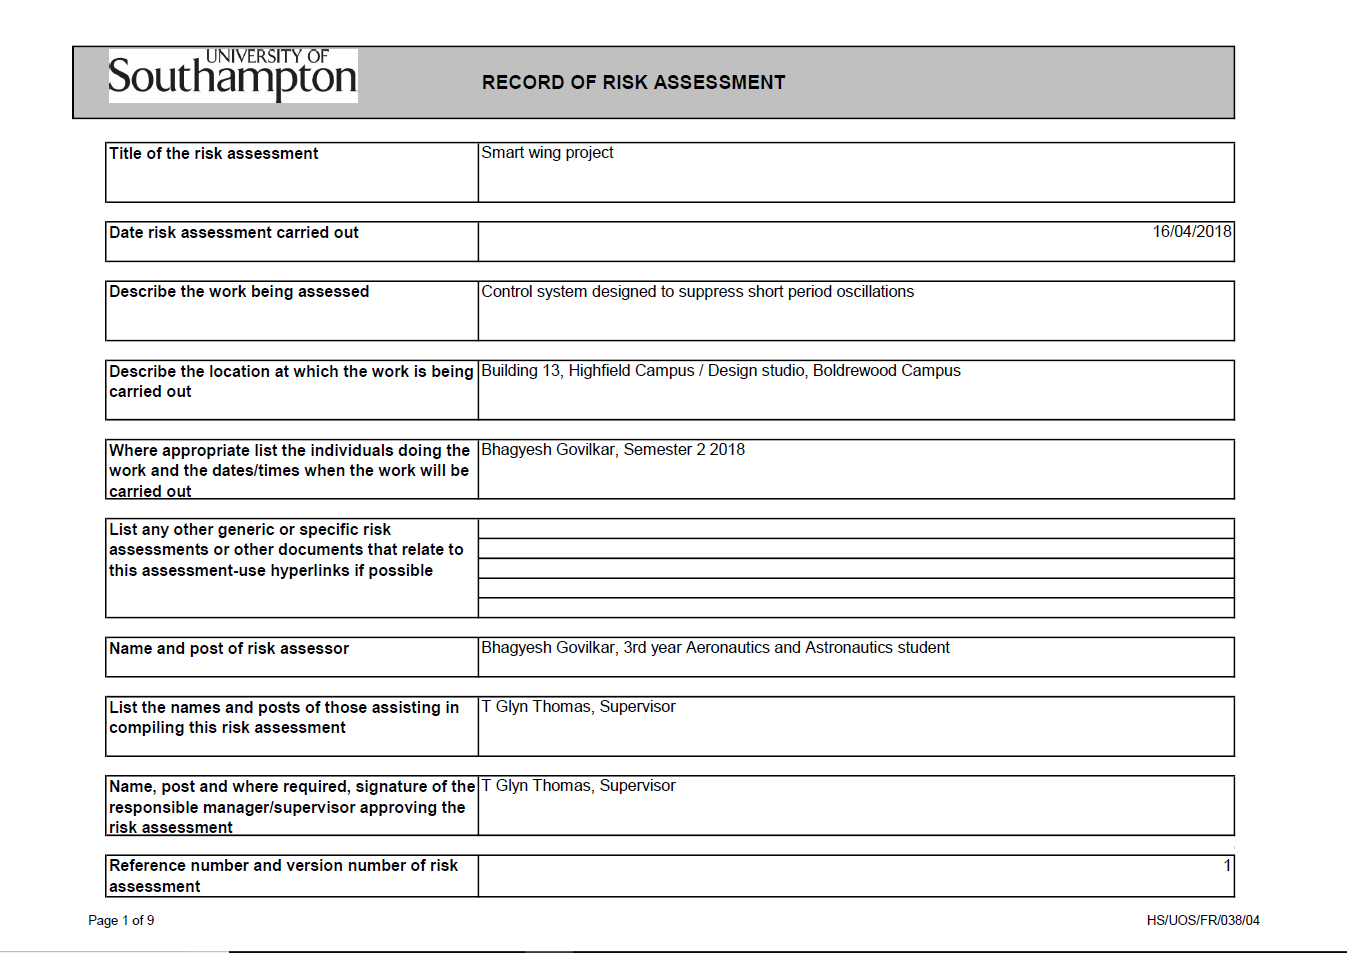
\includegraphics[scale=0.5]{ra1.png}
\caption{Section A}
\centering
\end{figure}
\newpage
\begin{sidewaysfigure}
\centering
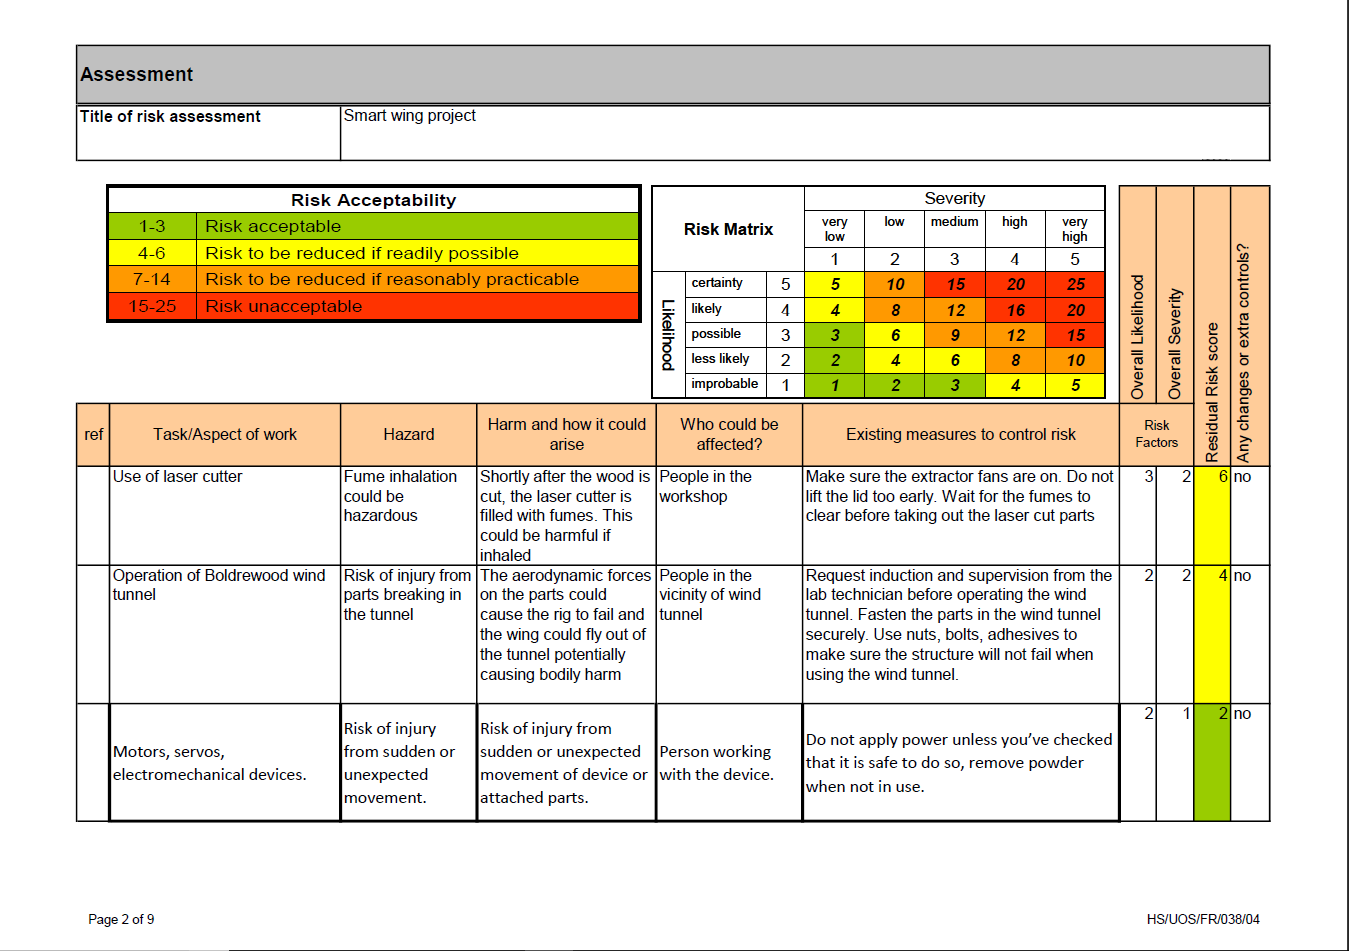
\includegraphics[scale=0.6]{ra2.png}
\caption{Section B}
\centering
\end{sidewaysfigure}
\newpage
\begin{sidewaysfigure}
\centering
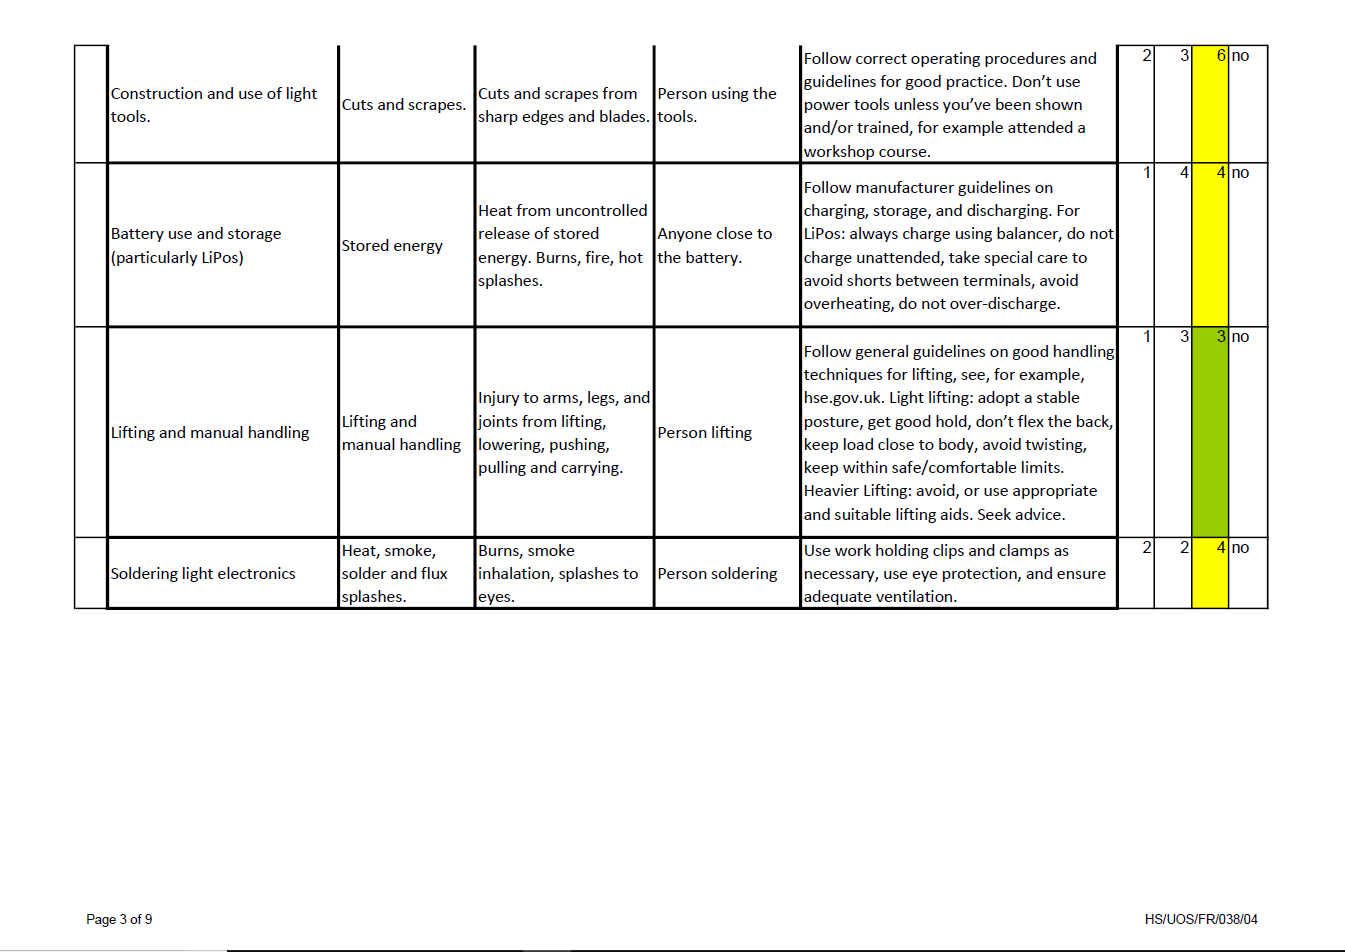
\includegraphics[scale=0.6]{ra3.png}
\caption{Section B}
\centering
\end{sidewaysfigure}
\newpage
\begin{sidewaysfigure}
\centering
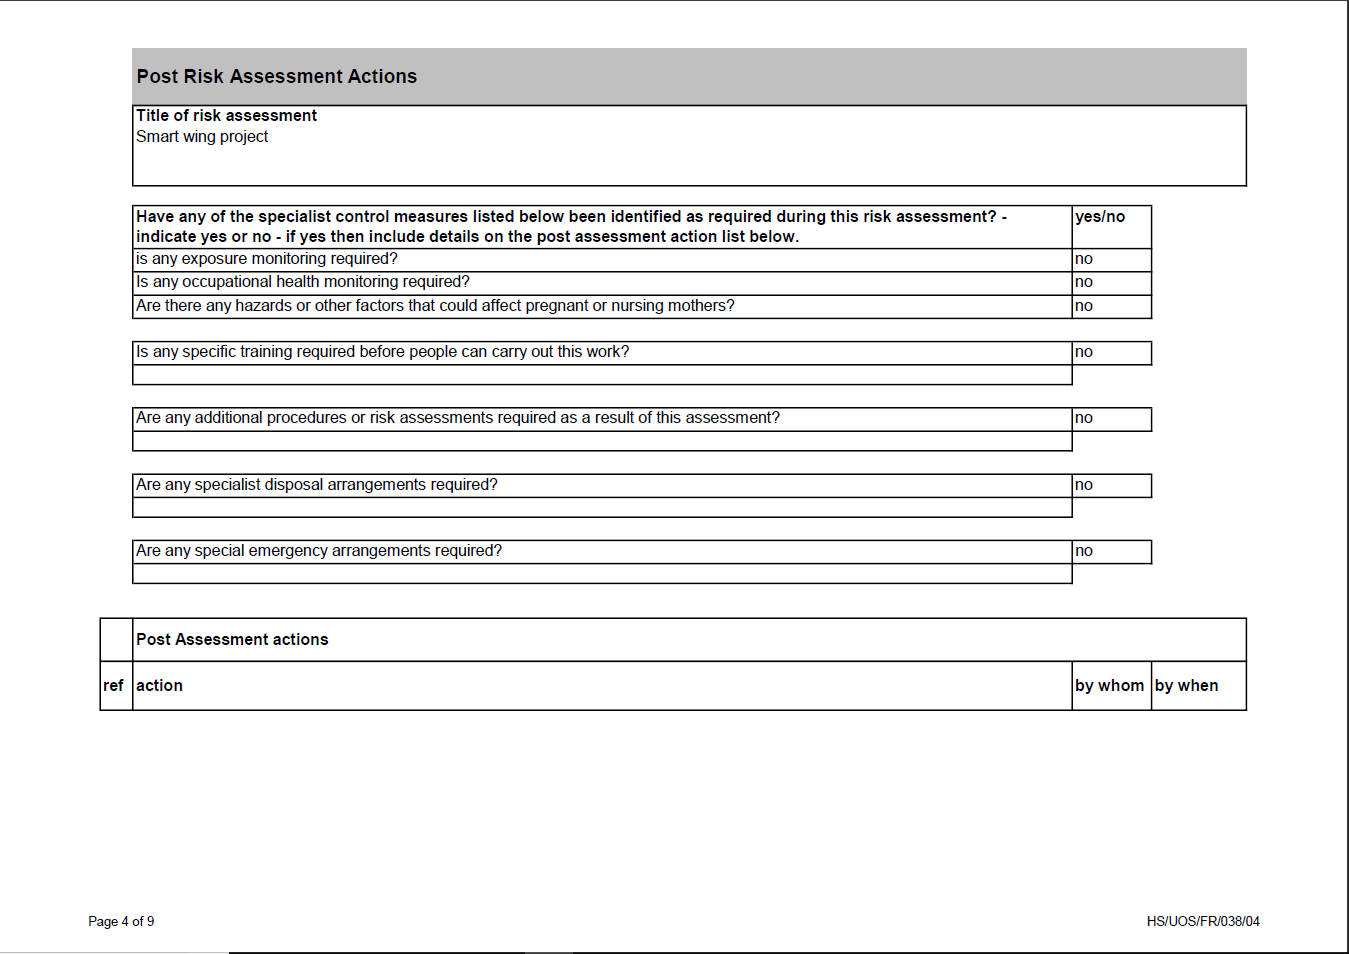
\includegraphics[scale=0.6]{ra4.png}
\caption{Section C}
\centering
\end{sidewaysfigure}

\chapter{Method Statement}
\thispagestyle{fancy}
This method statement is in reference to the project “Active Control of Wing Lift: Suppressing SPOs”. The scope of the work to be done is as follows: analysis of SPOs, design of controller, design of wing and the rig, building the wing, the rig and the gust generator and then finally testing the controller in a wind tunnel.
\newline
\newline
Most of the risk arises from manufacturing the parts and testing the controller in the wind tunnel. The wing will be split into four parts: the central section, the two ends of the wing and the movable trailing edge flap. The central section of the wing has pressure tappings which complicate the geometry of the part. 3D printing will therefore be necessary to produce this part. The ends of the wing are the same profile as the 3D printed parts. Due to the simple geometry of the part, the same profile can be laser cut several times and the laser cut parts can be stuck together side to side in order to extend the span of the wing. The flap will also be made similarly since all features of the flap are two dimensional. A RC servo will actuate the flap.
The wing will be mounted using some fixtures on the left and right walls of the wind tunnel. These are circular discs with holes in them for the carbon fibre rods and some more holes for the PVC tubes connected to the pressure tappings of the wing. These fixtures will be made exclusively by laser cutting.
\newline
\newline
The gust generator consists of two NACA0015 flaps which are 250mm in chord and 500mm in span. Due to the simple geometry, these can be foam cut. Laser cutting will be very inconvenient for this part due to the size of the flaps. The gust generator will operate by using two RC servos to deflect the flaps. Some carbon fibre rods will be used to provide structural support to the flaps. The rods will also serve as a shaft to connect the flap to the RC servos. The rods will be supported by a stand on either side of the flap as outlined in the diagram. These stands will be laser cut out of MDF.
\newline
\newline
Once the wing and gust generator is manufactured and mounted, the electronics need to be built. I will have to solder some differential pressure sensors onto a breadboard. These will be connected to a Raspberry Pi 3 (a microcontroller). The Raspberry Pi 3 will be connected to my laptop via WiFi through the Secure Shell protocol. This will allow me to monitor the data for my test. The Raspberry Pi will be running a code to implement my controller. It will use the pressure data to estimate the lift and remove the error by adjusting the flap angle through the RC servo mentioned above. The entire setup is outlined in the diagram on the next page.
\newline
\newline
The project will finish after testing the wing in the wind tunnel. I will use the Boldrewood wing tunnel (600mm by 400mm). I will firstly request induction and supervision from the lab supervisor. When testing, the wind tunnel will be turned on and the gust generator will be programmed to produce an impulsive gust by deflecting the flaps very quickly. The system should attempt to correct the lift change caused by the gust by moving the flap.
\begin{figure}[H]
\centering
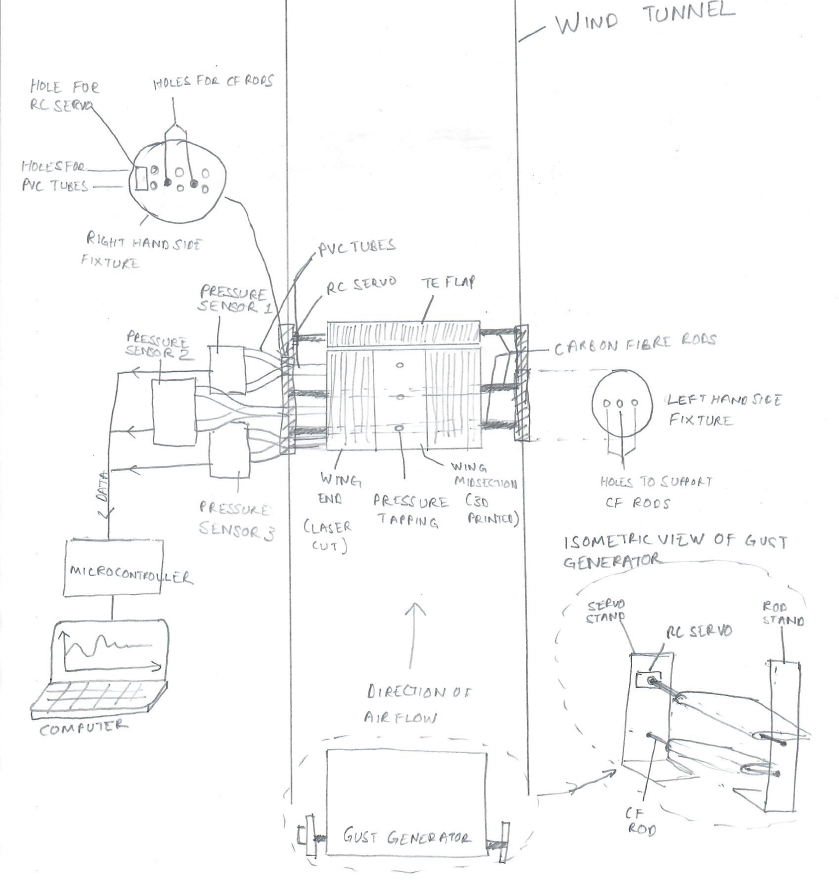
\includegraphics[scale=0.8]{msp.png}
\caption{Diagram of the setup}
\centering
\end{figure}
\chapter{Lift Estimator}
\thispagestyle{fancy}


\tiny
\begin{longtable}{|l|l|l|l|l|l|l|l|l|l|l|l|l|}
\caption{Lift estimator values and xfoil predicted values}
\label{tab:mylabel}
\tabularnewline
\hline
delta & alpha & Cp1     & Cp2     & Cp3     & p1       & p2       & p3       & Cl       & Actual Lift & Estimated Lift & Error\textasciicircum{}2 & \%Error     \\ \hline
0     & -5    & -0.5629 & -0.1619 & -0.0523 & -137.911 & -39.6655 & -12.8135 & -0.3757  & -2.485256   & -2.328769747   & 0.024488                 & 6.296565995 \\ \hline
0     & -4.5  & -0.4513 & -0.101  & -0.0122 & -110.569 & -24.745  & -2.989   & -0.3034  & -2.006991   & -1.84326134    & 0.026807                 & 8.157966835 \\ \hline
0     & -4    & -0.3476 & -0.0319 & 0.0351  & -85.162  & -7.8155  & 8.5995   & -0.223   & -1.475145   & -1.399489283   & 0.005724                 & 5.128696979 \\ \hline
0     & -3.5  & -0.3279 & 0.0311  & 0.0736  & -80.3355 & 7.6195   & 18.032   & -0.1551  & -1.025987   & -1.409230972   & 0.146876                 & 37.35375389 \\ \hline
0     & -3    & -0.2003 & 0.0998  & 0.1116  & -49.0735 & 24.451   & 27.342   & -0.0901  & -0.596012   & -0.897299727   & 0.090775                 & 50.55074051 \\ \hline
0     & -2.5  & -0.099  & 0.0947  & 0.1499  & -24.255  & 23.2015  & 36.7255  & -0.0306  & -0.202419   & -0.111006851   & 0.008356                 & 45.15986598 \\ \hline
0     & -2    & -0.01   & 0.1603  & 0.1742  & -2.45    & 39.2735  & 42.679   & 0.020367 & 0.1347255   & 0.134704751    & 4.31E-10                 & 0.01540107  \\ \hline
0     & -1.5  & 0.0744  & 0.2118  & 0.1779  & 18.228   & 51.891   & 43.5855  & 0.071333 & 0.47187     & 0.307820941    & 0.026912                 & 34.76573182 \\ \hline
0     & -1    & 0.1557  & 0.2578  & 0.2125  & 38.1465  & 63.161   & 52.0625  & 0.1223   & 0.8090145   & 0.685646144    & 0.01522                  & 15.24921447 \\ \hline
0     & -0.5  & 0.2402  & 0.3048  & 0.2465  & 58.849   & 74.676   & 60.3925  & 0.1734   & 1.147041    & 1.070744217    & 0.005821                 & 6.651617747 \\ \hline
0     & 0     & 0.3389  & 0.3626  & 0.2914  & 83.0305  & 88.837   & 71.393   & 0.2391   & 1.5816465   & 1.536447515    & 0.002043                 & 2.857717242 \\ \hline
0     & 0.5   & 0.4536  & 0.4322  & 0.3497  & 111.132  & 105.889  & 85.6765  & 0.3213   & 2.1253995   & 2.101900546    & 0.000552                 & 1.105625287 \\ \hline
0     & 1     & 0.5769  & 0.5086  & 0.417   & 141.3405 & 124.607  & 102.165  & 0.413    & 2.731995    & 2.729507842    & 6.19E-06                 & 0.091038158 \\ \hline
0     & 1.5   & 0.6637  & 0.5559  & 0.458   & 162.6065 & 136.1955 & 112.21   & 0.4685   & 3.0991275   & 3.167909238    & 0.004731                 & 2.219390401 \\ \hline
0     & 2     & 0.7423  & 0.5977  & 0.4959  & 181.8635 & 146.4365 & 121.4955 & 0.516    & 3.41334     & 3.575360908    & 0.026251                 & 4.746697009 \\ \hline
0     & 2.5   & 0.8211  & 0.641   & 0.5364  & 201.1695 & 157.045  & 131.418  & 0.5634   & 3.726891    & 3.991559243    & 0.070049                 & 7.101582601 \\ \hline
0     & 3     & 0.9001  & 0.6867  & 0.5217  & 220.5245 & 168.2415 & 127.8165 & 0.6109   & 4.0411035   & 4.055605192    & 0.00021                  & 0.358854756 \\ \hline
0     & 3.5   & 0.9791  & 0.7356  & 0.4583  & 239.8795 & 180.222  & 112.2835 & 0.6584   & 4.355316    & 3.802069646    & 0.306082                 & 12.70278331 \\ \hline
0     & 4     & 1.0583  & 0.7882  & 0.4727  & 259.2835 & 193.109  & 115.8115 & 0.7058   & 4.668867    & 4.008183434    & 0.436503                 & 14.15083286 \\ \hline
0     & 4.5   & 1.1376  & 0.8446  & 0.5056  & 278.712  & 206.927  & 123.872  & 0.753    & 4.981095    & 4.307719099    & 0.453435                 & 13.51863196 \\ \hline
0     & 5     & 1.2175  & 0.9047  & 0.5365  & 298.2875 & 221.6515 & 131.4425 & 0.8004   & 5.294646    & 4.577571966    & 0.514195                 & 13.54338013 \\ \hline
0     & 5.5   & 1.2981  & 0.9683  & 0.5642  & 318.0345 & 237.2335 & 138.229  & 0.8474   & 5.605551    & 4.811974158    & 0.629764                 & 14.15698193 \\ \hline
0     & 6     & 1.3801  & 0.9185  & 0.5891  & 338.1245 & 225.0325 & 144.3295 & 0.894    & 5.91381     & 5.663436156    & 0.062687                 & 4.233714715 \\ \hline
0     & 6.5   & 1.4644  & 0.9275  & 0.6113  & 358.778  & 227.2375 & 149.7685 & 0.9388   & 6.210162    & 6.184974825    & 0.000634                 & 0.405579992 \\ \hline
0     & 7     & 1.5562  & 0.9788  & 0.6301  & 381.269  & 239.806  & 154.3745 & 0.9809   & 6.4886535   & 6.490330372    & 2.81E-06                 & 0.025843141 \\ \hline
0     & 7.5   & 1.6219  & 1.0202  & 0.6452  & 397.3655 & 249.949  & 158.074  & 1.02     & 6.7473      & 6.693090432    & 0.002939                 & 0.803426084 \\ \hline
0     & 8     & 1.6171  & 1.0535  & 0.6567  & 396.1895 & 258.1075 & 160.8915 & 1.0566   & 6.989409    & 6.555015548    & 0.188698                 & 6.215024075 \\ \hline
0     & 8.5   & 1.6936  & 1.0822  & 0.6655  & 414.932  & 265.139  & 163.0475 & 1.0912   & 7.218288    & 6.844889064    & 0.139427                 & 5.172957019 \\ \hline
0     & 8     & 1.7583  & 1.1083  & 0.6721  & 430.7835 & 271.5335 & 164.6645 & 1.1245   & 7.4385675   & 7.07475877     & 0.132357                 & 4.890843973 \\ \hline
0     & 9.5   & 1.8145  & 1.1292  & 0.6737  & 444.5525 & 276.654  & 165.0565 & 1.1531   & 7.6277565   & 7.2587733      & 0.136149                 & 4.83737519  \\ \hline
0     & 10    & 2.1254  & 1.7566  & 1.7207  & 520.723  & 430.367  & 421.5715 & 1.1817   & 7.8169455   & 11.83941768    & 16.18028                 & 51.45836292 \\ \hline
15    & -5    & 0.4177  & 0.6491  & 0.7953  & 102.3365 & 159.0295 & 194.8485 & 0.728    & 4.81572     & 3.461323619    & 1.83439                  & 28.12448358 \\ \hline
15    & -4.5  & 0.5579  & 0.7427  & 0.8796  & 136.6855 & 181.9615 & 215.502  & 0.7856   & 5.196744    & 4.185627561    & 1.022356                 & 19.45672981 \\ \hline
15    & -4    & 0.7666  & 0.895   & 1.0023  & 187.817  & 219.275  & 245.5635 & 0.8432   & 5.577768    & 5.174937811    & 0.162272                 & 7.222067849 \\ \hline
15    & -3.5  & 0.8569  & 0.9405  & 1.0341  & 209.9405 & 230.4225 & 253.3545 & 0.9008   & 5.958792    & 5.584684986    & 0.139956                 & 6.278235821 \\ \hline
15    & -3    & 0.9472  & 0.9832  & 1.0652  & 232.064  & 240.884  & 260.974  & 0.9584   & 6.339816    & 6.005605243    & 0.111697                 & 5.271616034 \\ \hline
15    & -2.5  & 1.0045  & 1.0116  & 1.0731  & 246.1025 & 247.842  & 262.9095 & 0.9841   & 6.5098215   & 6.192611228    & 0.100622                 & 4.872795232 \\ \hline
15    & -2    & 1.0338  & 1.015   & 1.0337  & 253.281  & 248.675  & 253.2565 & 0.9804   & 6.485346    & 6.082245906    & 0.16249                  & 6.215552625 \\ \hline
15    & -1.5  & 1.0824  & 1.0342  & 1.0464  & 265.188  & 253.379  & 256.368  & 0.9971   & 6.5958165   & 6.304831666    & 0.084672                 & 4.411657513 \\ \hline
15    & -1    & 1.1377  & 1.0599  & 1.056   & 278.7365 & 259.6755 & 258.72   & 1.021    & 6.753915    & 6.506925645    & 0.061004                 & 3.656980506 \\ \hline
15    & -0.5  & 1.2023  & 1.0984  & 1.0691  & 294.5635 & 269.108  & 261.9295 & 1.054    & 6.97221     & 6.707735617    & 0.069947                 & 3.793264739 \\ \hline
15    & 0     & 1.2673  & 1.0869  & 1.0566  & 310.4885 & 266.2905 & 258.867  & 1.0864   & 7.186536    & 7.02945959     & 0.024673                 & 2.185704068 \\ \hline
15    & 0.5   & 1.3339  & 1.1346  & 1.0581  & 326.8055 & 277.977  & 259.2345 & 1.1218   & 7.420707    & 7.118275142    & 0.091465                 & 4.075512722 \\ \hline
15    & 1     & 1.4024  & 1.1728  & 1.0755  & 343.588  & 287.336  & 263.4975 & 1.1583   & 7.6621545   & 7.367328922    & 0.086922                 & 3.847815625 \\ \hline
15    & 1.5   & 1.4771  & 1.2083  & 1.0918  & 361.8895 & 296.0335 & 267.491  & 1.1952   & 7.906248    & 7.656503396    & 0.062372                 & 3.158825831 \\ \hline
15    & 2     & 1.5129  & 1.2449  & 1.1099  & 370.6605 & 305.0005 & 271.9255 & 1.2352   & 8.170848    & 7.75013252     & 0.177002                 & 5.148981838 \\ \hline
15    & 2.5   & 1.6046  & 1.2801  & 1.1276  & 393.127  & 313.6245 & 276.262  & 1.2757   & 8.4387555   & 8.137229375    & 0.090918                 & 3.573111281 \\ \hline
15    & 3     & 1.6818  & 1.3176  & 1.1455  & 412.041  & 322.812  & 280.6475 & 1.3177   & 8.7165855   & 8.438085282    & 0.077562                 & 3.195060935 \\ \hline
15    & 3.5   & 1.7543  & 1.3546  & 1.1633  & 429.8035 & 331.877  & 285.0085 & 1.3601   & 8.9970615   & 8.71685976     & 0.078513                 & 3.114369503 \\ \hline
15    & 4     & 1.8288  & 1.3906  & 1.1802  & 448.056  & 340.697  & 289.149  & 1.4026   & 9.278199    & 9.00593292     & 0.074129                 & 2.934471232 \\ \hline
15    & 4.5   & 1.9024  & 1.4263  & 1.1967  & 466.088  & 349.4435 & 293.1915 & 1.4451   & 9.5593365   & 9.289562006    & 0.072778                 & 2.822104797 \\ \hline
15    & 5     & 1.9747  & 1.462   & 1.2116  & 483.8015 & 358.19   & 296.842  & 1.4869   & 9.8358435   & 9.556636504    & 0.077957                 & 2.838668554 \\ \hline
15    & 5.5   & 2.0451  & 1.4971  & 1.2259  & 501.0495 & 366.7895 & 300.3455 & 1.5279   & 10.107059   & 9.813538877    & 0.086154                 & 2.904105316 \\ \hline
15    & 6     & 2.1167  & 1.5305  & 1.2389  & 518.5915 & 374.9725 & 303.5305 & 1.5684   & 10.374966   & 10.07802334    & 0.088175                 & 2.862107318 \\ \hline
15    & 6.5   & 2.1844  & 1.5625  & 1.2505  & 535.178  & 382.8125 & 306.3725 & 1.6073   & 10.63229    & 10.32152241    & 0.096576                 & 2.92286142  \\ \hline
15    & 7     & 2.2507  & 1.5934  & 1.2605  & 551.4215 & 390.383  & 308.8225 & 1.6454   & 10.884321   & 10.55403418    & 0.109089                 & 3.034519299 \\ \hline
15    & 7.5   & 2.3164  & 1.6236  & 1.2693  & 567.518  & 397.782  & 310.9785 & 1.6822   & 11.127753   & 10.77993418    & 0.120978                 & 3.125687794 \\ \hline
15    & 8     & 2.3806  & 1.6513  & 1.2764  & 583.247  & 404.5685 & 312.718  & 1.7176   & 11.361924   & 11.00145733    & 0.129936                 & 3.172584742 \\ \hline
15    & 8.5   & 2.4403  & 1.6774  & 1.2811  & 597.8735 & 410.963  & 313.8695 & 1.7509   & 11.582204   & 11.19384998    & 0.150818                 & 3.353019353 \\ \hline
15    & 9     & 2.4986  & 1.7021  & 1.2838  & 612.157  & 417.0145 & 314.531  & 1.7829   & 11.793884   & 11.37445113    & 0.175924                 & 3.556355003 \\ \hline
15    & 9.5   & 2.5559  & 1.7243  & 1.2848  & 626.1955 & 422.4535 & 314.776  & 1.8135   & 11.996303   & 11.55325316    & 0.196293                 & 3.693215816 \\ \hline
15    & 10    & 2.6103  & 1.7441  & 1.2826  & 639.5235 & 427.3045 & 314.237  & 1.8412   & 12.179538   & 11.71067099    & 0.219836                 & 3.849628825 \\ \hline
30    & -5    & 1.6576  & 1.6272  & 1.8181  & 406.112  & 398.664  & 445.4345 & 0.9964   & 6.591186    & 10.74303655    & 17.23786                 & 62.9909481  \\ \hline
30    & -4.5  & 1.5026  & 1.4945  & 1.6624  & 368.137  & 366.1525 & 407.288  & 1.0399   & 6.8789385   & 9.718980337    & 8.065838                 & 41.2860478  \\ \hline
30    & -4    & 1.4287  & 1.4285  & 1.5911  & 350.0315 & 349.9825 & 389.8195 & 1.0834   & 7.166691    & 9.263910112    & 4.398328                 & 29.26342313 \\ \hline
30    & -3.5  & 1.1681  & 1.1739  & 1.2518  & 286.1845 & 287.6055 & 306.691  & 1.1269   & 7.4544435   & 7.238950837    & 0.046437                 & 2.890794777 \\ \hline
30    & -3    & 1.2413  & 1.2164  & 1.2848  & 304.1185 & 298.018  & 314.776  & 1.1704   & 7.742196    & 7.584518907    & 0.024862                 & 2.036593916 \\ \hline
30    & -2.5  & 1.3197  & 1.2644  & 1.3101  & 323.3265 & 309.778  & 320.9745 & 1.2139   & 8.0299485   & 7.879065893    & 0.022766                 & 1.878998444 \\ \hline
30    & -2    & 1.4016  & 1.3162  & 1.3359  & 343.392  & 322.469  & 327.2955 & 1.2634   & 8.357391    & 8.173722429    & 0.033734                 & 2.197678335 \\ \hline
30    & -1.5  & 1.4808  & 1.3268  & 1.358   & 362.796  & 325.066  & 332.71   & 1.3091   & 8.6596965   & 8.659504826    & 3.67E-08                 & 0.002213403 \\ \hline
30    & -1    & 1.558   & 1.3779  & 1.3793  & 381.71   & 337.5855 & 337.9285 & 1.353    & 8.950095    & 8.906091479    & 0.001936                 & 0.491654229 \\ \hline
30    & -0.5  & 1.6451  & 1.4207  & 1.4018  & 403.0495 & 348.0715 & 343.441  & 1.398    & 9.24777     & 9.257004064    & 8.53E-05                 & 0.099851789 \\ \hline
30    & 0     & 1.6922  & 1.4636  & 1.424   & 414.589  & 358.582  & 348.88   & 1.4433   & 9.5474295   & 9.399298728    & 0.021943                 & 1.551525174 \\ \hline
30    & 0.5   & 1.7804  & 1.5014  & 1.4443  & 436.198  & 367.843  & 353.8535 & 1.4861   & 9.8305515   & 9.769984295    & 0.003668                 & 0.616111975 \\ \hline
30    & 1     & 1.856   & 1.54    & 1.4631  & 454.72   & 377.3    & 358.4595 & 1.5282   & 10.109043   & 10.06205071    & 0.002208                 & 0.464853965 \\ \hline
30    & 1.5   & 1.9291  & 1.5774  & 1.4778  & 472.6295 & 386.463  & 362.061  & 1.5701   & 10.386212   & 10.32261727    & 0.004044                 & 0.612294813 \\ \hline
30    & 2     & 2.0044  & 1.6137  & 1.4835  & 491.078  & 395.3565 & 363.4575 & 1.6116   & 10.660734   & 10.5451882     & 0.013351                 & 1.08384468  \\ \hline
30    & 2.5   & 2.0787  & 1.6495  & 1.467   & 509.2815 & 404.1275 & 359.415  & 1.6526   & 10.931949   & 10.62866494    & 0.091981                 & 2.774290851 \\ \hline
30    & 3     & 2.1499  & 1.6842  & 1.4779  & 526.7255 & 412.629  & 362.0855 & 1.6925   & 11.195888   & 10.870967      & 0.105573                 & 2.902141511 \\ \hline
30    & 3.5   & 2.2209  & 1.7179  & 1.493   & 544.1205 & 420.8855 & 365.785  & 1.7315   & 11.453873   & 11.14363068    & 0.09625                  & 2.708619499 \\ \hline
30    & 4     & 2.2893  & 1.7496  & 1.5061  & 560.8785 & 428.652  & 368.9945 & 1.7692   & 11.703258   & 11.40163424    & 0.090977                 & 2.577263144 \\ \hline
30    & 4.5   & 2.3546  & 1.7811  & 1.5179  & 576.877  & 436.3695 & 371.8855 & 1.8057   & 11.944706   & 11.63675675    & 0.094832                 & 2.578119246 \\ \hline
30    & 5     & 2.421   & 1.81    & 1.5278  & 593.145  & 443.45   & 374.311  & 1.8409   & 12.177554   & 11.88022796    & 0.088402                 & 2.441586801 \\ \hline
30    & 5.5   & 2.4823  & 1.8377  & 1.5357  & 608.1635 & 450.2365 & 376.2465 & 1.8746   & 12.400479   & 12.09172659    & 0.095328                 & 2.489842574 \\ \hline
30    & 6     & 2.5465  & 1.863   & 1.5406  & 623.8925 & 456.435  & 377.447  & 1.906    & 12.60819    & 12.31297415    & 0.087152                 & 2.341460955 \\ \hline
30    & 6.5   & 2.6051  & 1.8871  & 1.5447  & 638.2495 & 462.3395 & 378.4515 & 1.9371   & 12.813917   & 12.5070608     & 0.09416                  & 2.394706545 \\ \hline
30    & 7     & 2.662   & 1.9092  & 1.5449  & 652.19   & 467.754  & 378.5005 & 1.9654   & 13.001121   & 12.67942738    & 0.103487                 & 2.474352964 \\ \hline
30    & 7.5   & 2.7149  & 1.9276  & 1.5407  & 665.1505 & 472.262  & 377.4715 & 1.9903   & 13.165835   & 12.82453819    & 0.116483                 & 2.592287748 \\ \hline
30    & 8     & 2.7652  & 1.9429  & 1.5336  & 677.474  & 476.0105 & 375.732  & 2.0132   & 13.317318   & 12.95552967    & 0.130891                 & 2.716675588 \\ \hline
30    & 8.5   & 2.8135  & 1.9586  & 1.5265  & 689.3075 & 479.857  & 373.9925 & 2.0367   & 13.472771   & 13.07399834    & 0.159019                 & 2.959837814 \\ \hline
30    & 9     & 2.8571  & 1.969   & 1.5121  & 699.9895 & 482.405  & 370.4645 & 2.055    & 13.593825   & 13.1525925     & 0.194686                 & 3.245830361 \\ \hline
30    & 9.5   & 2.8951  & 1.975   & 1.4924  & 709.2995 & 483.875  & 365.638  & 2.0698   & 13.691727   & 13.19401104    & 0.247721                 & 3.635158396 \\ \hline
30    & 10    & 2.935   & 1.982   & 1.474   & 719.075  & 485.59   & 361.13   & 2.0867   & 13.803521   & 13.24770024    & 0.308936                 & 4.02665584  \\ \hline
45    & -5    & 2.0434  & 1.952   & 2.1479  & 500.633  & 478.24   & 526.2355 & 1.3171   & 8.7126165   & 12.96676264    & 18.09776                 & 48.82742333 \\ \hline
45    & -4.5  & 1.9784  & 1.8978  & 2.0908  & 484.708  & 464.961  & 512.246  & 1.3595   & 8.9930925   & 12.57976479    & 12.86422                 & 39.88252412 \\ \hline
45    & -4    & 1.9245  & 1.8549  & 2.0427  & 471.5025 & 454.4505 & 500.4615 & 1.4019   & 9.2735685   & 12.2429255     & 8.817081                 & 32.01957266 \\ \hline
45    & -3.5  & 1.888   & 1.8055  & 1.9825  & 462.56   & 442.3475 & 485.7125 & 1.4443   & 9.5540445   & 11.95722519    & 5.775277                 & 25.15354293 \\ \hline
45    & -3    & 1.834   & 1.7343  & 1.8848  & 449.33   & 424.9035 & 461.776  & 1.4867   & 9.8345205   & 11.47093685    & 2.677858                 & 16.63951334 \\ \hline
45    & -2.5  & 1.7773  & 1.6115  & 1.6686  & 435.4385 & 394.8175 & 408.807  & 1.5291   & 10.114997   & 10.52636661    & 0.169225                 & 4.066932771 \\ \hline
45    & -2    & 1.8208  & 1.6509  & 1.6843  & 446.096  & 404.4705 & 412.6535 & 1.5715   & 10.395473   & 10.62943028    & 0.054736                 & 2.250573832 \\ \hline
45    & -1.5  & 1.9057  & 1.6898  & 1.6993  & 466.8965 & 414.001  & 416.3285 & 1.6134   & 10.672641   & 10.94438361    & 0.073844                 & 2.546160874 \\ \hline
45    & -1    & 1.9805  & 1.7271  & 1.7121  & 485.2225 & 423.1395 & 419.4645 & 1.6533   & 10.93658    & 11.20256753    & 0.07075                  & 2.432095241 \\ \hline
45    & -0.5  & 2.053   & 1.7623  & 1.7236  & 502.985  & 431.7635 & 422.282  & 1.6921   & 11.193242   & 11.45250144    & 0.067216                 & 2.316218554 \\ \hline
45    & 0     & 2.1234  & 1.7959  & 1.7339  & 520.233  & 439.9955 & 424.8055 & 1.7298   & 11.442627   & 11.69306728    & 0.06272                  & 2.188660691 \\ \hline
45    & 0.5   & 2.1931  & 1.8287  & 1.7432  & 537.3095 & 448.0315 & 427.084  & 1.7667   & 11.686721   & 11.92829036    & 0.058356                 & 2.067045792 \\ \hline
45    & 1     & 2.2619  & 1.8599  & 1.7518  & 554.1655 & 455.6755 & 429.191  & 1.8024   & 11.922876   & 12.16341082    & 0.057857                 & 2.01742285  \\ \hline
45    & 1.5   & 2.3277  & 1.8892  & 1.7583  & 570.2865 & 462.854  & 430.7835 & 1.8368   & 12.150432   & 12.38064024    & 0.052996                 & 1.894650634 \\ \hline
45    & 2     & 2.3917  & 1.9186  & 1.7633  & 585.9665 & 470.057  & 432.0085 & 1.8696   & 12.367404   & 12.57880014    & 0.044688                 & 1.709300821 \\ \hline
45    & 2.5   & 2.4531  & 1.9445  & 1.7658  & 601.0095 & 476.4025 & 432.621  & 1.9004   & 12.571146   & 12.76751578    & 0.038561                 & 1.562067492 \\ \hline
45    & 3     & 2.5151  & 1.9691  & 1.767   & 616.1995 & 482.4295 & 432.915  & 1.9301   & 12.767612   & 12.95850832    & 0.036442                 & 1.495164698 \\ \hline
45    & 3.5   & 2.5735  & 1.9917  & 1.7668  & 630.5075 & 487.9665 & 432.866  & 1.9583   & 12.954155   & 13.13338       & 0.032122                 & 1.383536867 \\ \hline
45    & 4     & 2.63    & 2.0135  & 1.764   & 644.35   & 493.3075 & 432.18   & 1.9851   & 13.131437   & 13.28686988    & 0.02416                  & 1.183673882 \\ \hline
45    & 4.5   & 2.6848  & 2.0334  & 1.7597  & 657.776  & 498.183  & 431.1265 & 2.0104   & 13.298796   & 13.43286548    & 0.017975                 & 1.008132482 \\ \hline
45    & 5     & 2.7338  & 2.0494  & 1.7494  & 669.781  & 502.103  & 428.603  & 2.0317   & 13.439696   & 13.53357897    & 0.008814                 & 0.698553577 \\ \hline
45    & 5.5   & 2.7862  & 2.0646  & 1.7386  & 682.619  & 505.827  & 425.957  & 2.0538   & 13.585887   & 13.65316592    & 0.004526                 & 0.495211849 \\ \hline
45    & 6     & 2.8305  & 2.0742  & 1.7189  & 693.4725 & 508.179  & 421.1305 & 2.0706   & 13.697019   & 13.7071563     & 0.000103                 & 0.074010968 \\ \hline
45    & 6.5   & 2.8754  & 2.0863  & 1.6969  & 704.473  & 511.1435 & 415.7405 & 2.0896   & 13.822704   & 13.73625234    & 0.007474                 & 0.625432367 \\ \hline
45    & 7     & 2.9151  & 2.0924  & 1.6674  & 714.1995 & 512.638  & 408.513  & 2.104    & 13.91796    & 13.72553546    & 0.037027                 & 1.382562786 \\ \hline
45    & 7.5   & 2.9506  & 2.0948  & 1.6262  & 722.897  & 513.226  & 398.419  & 2.1152   & 13.992048   & 13.64157963    & 0.122828                 & 2.504768216 \\ \hline
45    & 8     & 2.9859  & 2.0968  & 1.5853  & 731.5455 & 513.716  & 388.3985 & 2.1275   & 14.073413   & 13.56065199    & 0.262923                 & 3.643469634 \\ \hline
45    & 8.5   & 3.0167  & 2.0946  & 1.5436  & 739.0915 & 513.177  & 378.182  & 2.1367   & 14.134271   & 13.47482395    & 0.43487                  & 4.665586039 \\ \hline
45    & 9     & 3.038   & 2.0853  & 1.4983  & 744.31   & 510.8985 & 367.0835 & 2.1408   & 14.161392   & 13.35711295    & 0.646865                 & 5.679378512 \\ \hline
45    & 9.5   & 3.0624  & 2.0738  & 1.4491  & 750.288  & 508.081  & 355.0295 & 2.1453   & 14.19116    & 13.24353395    & 0.897994                 & 6.677576647 \\ \hline
45    & 10    & 3.0852  & 2.0613  & 1.3962  & 755.874  & 505.0185 & 342.069  & 2.1502   & 14.223573   & 13.10445214    & 1.252431                 & 7.86807126  \\ \hline
60    & -5    & 2.8981  & 2.6236  & 2.7989  & 710.0345 & 642.782  & 685.7305 & 1.5257   & 10.092506   & 17.66801805    & 57.38839                 & 75.06077212 \\ \hline
60    & -4.5  & 2.0694  & 1.9289  & 2.0895  & 507.003  & 472.5805 & 511.9275 & 1.5613   & 10.328      & 12.86892654    & 6.45631                  & 24.60231568 \\ \hline
60    & -4    & 2.0209  & 1.8818  & 2.031   & 495.1205 & 461.041  & 497.595  & 1.5969   & 10.563494   & 12.51911061    & 3.824438                 & 18.51297686 \\ \hline
60    & -3.5  & 1.9676  & 1.8034  & 1.9045  & 482.062  & 441.833  & 466.6025 & 1.6325   & 10.798988   & 11.89890063    & 1.209809                 & 10.1853357  \\ \hline
60    & -3    & 2.0345  & 1.8354  & 1.9131  & 498.4525 & 449.673  & 468.7095 & 1.6681   & 11.034482   & 12.11980188    & 1.17792                  & 9.83571707  \\ \hline
60    & -2.5  & 2.104   & 1.87    & 1.9244  & 515.48   & 458.15   & 471.478  & 1.7037   & 11.269976   & 12.35635581    & 1.180222                 & 9.639597786 \\ \hline
60    & -2    & 2.1718  & 1.904   & 1.9321  & 532.091  & 466.48   & 473.3645 & 1.7384   & 11.499516   & 12.56529523    & 1.135885                 & 9.268035546 \\ \hline
60    & -1.5  & 2.2379  & 1.936   & 1.9377  & 548.2855 & 474.32   & 474.7365 & 1.7721   & 11.722442   & 12.76359866    & 1.084008                 & 8.881743276 \\ \hline
60    & -1    & 2.3036  & 1.9658  & 1.9405  & 564.382  & 481.621  & 475.4225 & 1.8029   & 11.926184   & 12.95476366    & 1.057977                 & 8.624554202 \\ \hline
60    & -0.5  & 2.3633  & 1.9935  & 1.9401  & 579.0085 & 488.4075 & 475.3245 & 1.8328   & 12.123972   & 13.10690366    & 0.966155                 & 8.107340199 \\ \hline
60    & 0     & 2.4253  & 2.0194  & 1.9376  & 594.1985 & 494.753  & 474.712  & 1.8645   & 12.333668   & 13.26792345    & 0.872834                 & 7.574843    \\ \hline
60    & 0.5   & 2.485   & 2.0432  & 1.9348  & 608.825  & 500.584  & 474.026  & 1.8926   & 12.519549   & 13.42685105    & 0.823197                 & 7.247082566 \\ \hline
60    & 1     & 2.5439  & 2.0664  & 1.9303  & 623.2555 & 506.268  & 472.9235 & 1.9198   & 12.699477   & 13.57450391    & 0.765672                 & 6.89025942  \\ \hline
60    & 1.5   & 2.5991  & 2.0871  & 1.9226  & 636.7795 & 511.3395 & 471.037  & 1.9463   & 12.874775   & 13.69720121    & 0.676386                 & 6.38789216  \\ \hline
60    & 2     & 2.6515  & 2.1055  & 1.9118  & 649.6175 & 515.8475 & 468.391  & 1.9693   & 13.02692    & 13.79909266    & 0.596251                 & 5.927519278 \\ \hline
60    & 2.5   & 2.7039  & 2.1223  & 1.9     & 662.4555 & 519.9635 & 465.5    & 1.9915   & 13.173773   & 13.90367404    & 0.532756                 & 5.540565866 \\ \hline
60    & 3     & 2.7536  & 2.138   & 1.8838  & 674.632  & 523.81   & 461.531  & 2.0136   & 13.319964   & 13.97332414    & 0.426879                 & 4.905119384 \\ \hline
60    & 3.5   & 2.8005  & 2.1498  & 1.8686  & 686.1225 & 526.701  & 457.807  & 2.0317   & 13.439696   & 14.05626321    & 0.380156                 & 4.587661277 \\ \hline
60    & 4     & 2.8472  & 2.1607  & 1.8466  & 697.564  & 529.3715 & 452.417  & 2.0504   & 13.563396   & 14.10127485    & 0.289314                 & 3.965664994 \\ \hline
60    & 4.5   & 2.8864  & 2.1679  & 1.8244  & 707.168  & 531.1355 & 446.978  & 2.0652   & 13.661298   & 14.12684954    & 0.216738                 & 3.407813381 \\ \hline
60    & 5     & 2.9289  & 2.175   & 1.796   & 717.5805 & 532.875  & 440.02   & 2.081    & 13.765815   & 14.13181167    & 0.133954                 & 2.658735901 \\ \hline
60    & 5.5   & 2.9654  & 2.1775  & 1.7661  & 726.523  & 533.4875 & 432.6945 & 2.0929   & 13.844534   & 14.12204169    & 0.077011                 & 2.004460388 \\ \hline
60    & 6     & 2.9975  & 2.176   & 1.7282  & 734.3875 & 533.12   & 423.409  & 2.1026   & 13.908699   & 14.06244456    & 0.023638                 & 1.105391387 \\ \hline
60    & 6.5   & 3.0307  & 2.1759  & 1.6877  & 742.5215 & 533.0955 & 413.4865 & 2.1138   & 13.982787   & 13.9847663     & 3.92E-06                 & 0.014155228 \\ \hline
60    & 7     & 3.0584  & 2.1706  & 1.6434  & 749.308  & 531.797  & 402.633  & 2.122    & 14.03703    & 13.88408856    & 0.023391                 & 1.089556968 \\ \hline
60    & 7.5   & 3.0848  & 2.1614  & 1.59    & 755.776  & 529.543  & 389.55   & 2.1282   & 14.078043   & 13.74223895    & 0.112764                 & 2.385303502 \\ \hline
60    & 8     & 3.102   & 2.1449  & 1.5254  & 759.99   & 525.5005 & 373.723  & 2.1306   & 14.093919   & 13.52435951    & 0.324398                 & 4.041171851 \\ \hline
60    & 8.5   & 3.1239  & 2.1291  & 1.4662  & 765.3555 & 521.6295 & 359.219  & 2.1348   & 14.121702   & 13.360092      & 0.58005                  & 5.393188429 \\ \hline
60    & 9     & 3.1387  & 2.1082  & 1.404   & 768.9815 & 516.509  & 343.98   & 2.1372   & 14.137578   & 13.16894959    & 0.938241                 & 6.851445182 \\ \hline
60    & 9.5   & 3.1515  & 2.0817  & 1.344   & 772.1175 & 510.0165 & 329.28   & 2.1387   & 14.147501   & 13.01201063    & 1.289337                 & 8.026081125 \\ \hline
60    & 10    & 3.1578  & 2.047   & 1.3008  & 773.661  & 501.515  & 318.696  & 2.1367   & 14.134271   & 12.97035745    & 1.354694                 & 8.234687791 \\ \hline
-15   & -5    & -1.5325 & -0.9498 & -0.8876 & -375.463 & -232.701 & -217.462 & -1.2972  & -8.580978   & -8.114151402   & 0.217927                 & 5.440249328 \\ \hline
-15   & -4.5  & -1.4534 & -0.9063 & -0.8626 & -356.083 & -222.044 & -211.337 & -1.245   & -8.235675   & -7.792958666   & 0.195998                 & 5.375592573 \\ \hline
-15   & -4    & -1.3735 & -0.8624 & -0.8371 & -336.508 & -211.288 & -205.09  & -1.1924  & -7.887726   & -7.466774604   & 0.1772                   & 5.336790298 \\ \hline
-15   & -3.5  & -1.2929 & -0.8183 & -0.8121 & -316.761 & -200.484 & -198.965 & -1.1396  & -7.538454   & -7.141166614   & 0.157837                 & 5.270144062 \\ \hline
-15   & -3    & -1.212  & -0.7733 & -0.7867 & -296.94  & -189.459 & -192.742 & -1.0865  & -7.187198   & -6.816525721   & 0.137398                 & 5.157389638 \\ \hline
-15   & -2.5  & -1.131  & -0.7287 & -0.761  & -277.095 & -178.532 & -186.445 & -1.0333  & -6.83528    & -6.48731       & 0.121083                 & 5.090786709 \\ \hline
-15   & -2    & -1.0478 & -0.6837 & -0.7353 & -256.711 & -167.507 & -180.149 & -0.9798  & -6.481377   & -6.148964248   & 0.110498                 & 5.128736564 \\ \hline
-15   & -1.5  & -0.9662 & -0.6381 & -0.7095 & -236.719 & -156.335 & -173.828 & -0.9263  & -6.127475   & -5.821569323   & 0.093578                 & 4.99235333  \\ \hline
-15   & -1    & -0.8834 & -0.5924 & -0.6832 & -216.433 & -145.138 & -167.384 & -0.8724  & -5.770926   & -5.485461942   & 0.08149                  & 4.94659016  \\ \hline
-15   & -0.5  & -0.8007 & -0.5459 & -0.6569 & -196.172 & -133.746 & -160.941 & -0.8186  & -5.415039   & -5.15429398    & 0.067988                 & 4.815201153 \\ \hline
-15   & 0     & -0.7158 & -0.4991 & -0.6304 & -175.371 & -122.28  & -154.448 & -0.7645  & -5.057168   & -4.812211437   & 0.060003                 & 4.843740345 \\ \hline
-15   & 0.5   & -0.633  & -0.4481 & -0.6039 & -155.085 & -109.785 & -147.956 & -0.7105  & -4.699958   & -4.504180656   & 0.038329                 & 4.165502441 \\ \hline
-15   & 1     & -0.5488 & -0.4199 & -0.5768 & -134.456 & -102.876 & -141.316 & -0.6558  & -4.338117   & -4.059157164   & 0.077819                 & 6.430435974 \\ \hline
-15   & 1.5   & -0.463  & -0.3702 & -0.5498 & -113.435 & -90.699  & -134.701 & -0.601   & -3.975615   & -3.725392356   & 0.062611                 & 6.293935496 \\ \hline
-15   & 2     & -0.379  & -0.3189 & -0.5225 & -92.855  & -78.1305 & -128.013 & -0.5461  & -3.612452   & -3.407907741   & 0.041838                 & 5.662187002 \\ \hline
-15   & 2.5   & -0.2943 & -0.2702 & -0.4952 & -72.1035 & -66.199  & -121.324 & -0.4914  & -3.250611   & -3.072436728   & 0.031746                 & 5.481254823 \\ \hline
-15   & 3     & -0.2083 & -0.2228 & -0.4677 & -51.0335 & -54.586  & -114.587 & -0.4362  & -2.885463   & -2.721843284   & 0.026771                 & 5.670483948 \\ \hline
-15   & 3.5   & -0.1226 & -0.1757 & -0.4404 & -30.037  & -43.0465 & -107.898 & -0.3812  & -2.521638   & -2.372369084   & 0.022281                 & 5.919522005 \\ \hline
-15   & 4     & -0.0371 & -0.1276 & -0.4126 & -9.0895  & -31.262  & -101.087 & -0.3258  & -2.155167   & -2.026376902   & 0.016587                 & 5.975875558 \\ \hline
-15   & 4.5   & 0.0487  & -0.08   & -0.3853 & 11.9315  & -19.6    & -94.3985 & -0.2707  & -1.790681   & -1.679152079   & 0.012439                 & 6.228270255 \\ \hline
-15   & 5     & 0.1348  & -0.0325 & -0.3572 & 33.026   & -7.9625  & -87.514  & -0.2149  & -1.421564   & -1.324901381   & 0.009344                 & 6.799704605 \\ \hline
-15   & 5.5   & 0.2346  & 0.0157  & -0.3291 & 57.477   & 3.8465   & -80.6295 & -0.1588  & -1.050462   & -0.903892049   & 0.021483                 & 13.95290371 \\ \hline
-15   & 6     & 0.2959  & 0.0635  & -0.3007 & 72.4955  & 15.5575  & -73.6715 & -0.1024  & -0.677376   & -0.677307862   & 4.64E-09                 & 0.010059167 \\ \hline
-15   & 6.5   & 0.3864  & 0.1113  & -0.2729 & 94.668   & 27.2685  & -66.8605 & -0.0461  & -0.304952   & -0.303879529   & 1.15E-06                 & 0.351521911 \\ \hline
-15   & 7     & 0.4761  & 0.1578  & -0.2443 & 116.6445 & 38.661   & -59.8535 & 0.0102   & 0.067473    & 0.077539506    & 0.000101                 & 14.91930995 \\ \hline
-15   & 7.5   & 0.5618  & 0.2072  & -0.2165 & 137.641  & 50.764   & -53.0425 & 0.066    & 0.43659     & 0.417373981    & 0.000369                 & 4.401387826 \\ \hline
-15   & 8     & 0.6458  & 0.2619  & -0.188  & 158.221  & 64.1655  & -46.06   & 0.12255  & 0.8106683   & 0.723446521    & 0.007608                 & 10.75923827 \\ \hline
-15   & 8.5   & 0.7319  & 0.3011  & -0.1599 & 179.3155 & 73.7695  & -39.1755 & 0.1791   & 1.1847465   & 1.123594909    & 0.00374                  & 5.161576015 \\ \hline
-15   & 9     & 0.816   & 0.3466  & -0.1312 & 199.92   & 84.917   & -32.144  & 0.23565  & 1.5588248   & 1.482289105    & 0.005858                 & 4.909829955 \\ \hline
-15   & 9.5   & 0.9018  & 0.394   & -0.1008 & 220.941  & 96.53    & -24.696  & 0.2922   & 1.932903    & 1.849709149    & 0.006921                 & 4.304088231 \\ \hline
-15   & 10    & 0.9354  & 0.4119  & -0.0862 & 229.173  & 100.9155 & -21.119  & 0.34875  & 2.3069813   & 2.013851972    & 0.085925                 & 12.7061838  \\ \hline
-30   & -5    & -2.0184 & -1.3441 & -1.3023 & -494.508 & -329.305 & -319.064 & -1.7167  & -11.35597   & -10.99241219   & 0.132175                 & 3.201472836 \\ \hline
-30   & -4.5  & -1.9454 & -1.3052 & -1.2828 & -476.623 & -319.774 & -314.286 & -1.6698  & -11.04573   & -10.71109839   & 0.111976                 & 3.029484696 \\ \hline
-30   & -4    & -1.872  & -1.2659 & -1.263  & -458.64  & -310.146 & -309.435 & -1.6229  & -10.73548   & -10.42808701   & 0.094493                 & 2.863368877 \\ \hline
-30   & -3.5  & -1.7979 & -1.2275 & -1.2431 & -440.486 & -300.738 & -304.56  & -1.5757  & -10.42326   & -10.13587417   & 0.082588                 & 2.757116773 \\ \hline
-30   & -3    & -1.7215 & -1.1858 & -1.2216 & -421.768 & -290.521 & -299.292 & -1.5269  & -10.10044   & -9.840199792   & 0.067727                 & 2.576557236 \\ \hline
-30   & -2.5  & -1.6461 & -1.145  & -1.1999 & -403.295 & -280.525 & -293.976 & -1.4782  & -9.778293   & -9.543472427   & 0.055141                 & 2.401447502 \\ \hline
-30   & -2    & -1.5689 & -1.1042 & -1.1786 & -384.381 & -270.529 & -288.757 & -1.4299  & -9.458789   & -9.2399284     & 0.0479                   & 2.313828036 \\ \hline
-30   & -1.5  & -1.4924 & -1.0634 & -1.1573 & -365.638 & -260.533 & -283.539 & -1.3818  & -9.140607   & -8.93999318    & 0.040246                 & 2.194753801 \\ \hline
-30   & -1    & -1.415  & -1.0218 & -1.1361 & -346.675 & -250.341 & -278.345 & -1.3335  & -8.821103   & -8.640457721   & 0.032633                 & 2.047870759 \\ \hline
-30   & -0.5  & -1.339  & -0.9805 & -1.1145 & -328.055 & -240.223 & -273.053 & -1.285   & -8.500275   & -8.344017796   & 0.024416                 & 1.838260577 \\ \hline
-30   & 0     & -1.2584 & -0.9372 & -1.0908 & -308.308 & -229.614 & -267.246 & -1.2347  & -8.167541   & -8.021991103   & 0.021185                 & 1.78204684  \\ \hline
-30   & 0.5   & -1.1805 & -0.8949 & -1.0677 & -289.223 & -219.251 & -261.587 & -1.1852  & -7.840098   & -7.712048949   & 0.016397                 & 1.633258301 \\ \hline
-30   & 1     & -1.1016 & -0.8513 & -1.0457 & -269.892 & -208.569 & -256.197 & -1.1363  & -7.516625   & -7.410913755   & 0.011175                 & 1.406359259 \\ \hline
-30   & 1.5   & -1.0242 & -0.8036 & -1.0235 & -250.929 & -196.882 & -250.758 & -1.0874  & -7.193151   & -7.13895251    & 0.002937                 & 0.753473551 \\ \hline
-30   & 2     & -0.9441 & -0.7787 & -1.0012 & -231.305 & -190.782 & -245.294 & -1.0386  & -6.870339   & -6.726375394   & 0.020726                 & 2.095436713 \\ \hline
-30   & 2.5   & -0.8656 & -0.7334 & -0.9789 & -212.072 & -179.683 & -239.831 & -0.9895  & -6.545543   & -6.434855762   & 0.012252                 & 1.69102467  \\ \hline
-30   & 3     & -0.7838 & -0.6876 & -0.9546 & -192.031 & -168.462 & -233.877 & -0.9387  & -6.209501   & -6.116772452   & 0.008598                 & 1.493325399 \\ \hline
-30   & 3.5   & -0.7044 & -0.6417 & -0.9301 & -172.578 & -157.217 & -227.875 & -0.8877  & -5.872136   & -5.810383617   & 0.003813                 & 1.051608616 \\ \hline
-30   & 4     & -0.6242 & -0.5986 & -0.9071 & -152.929 & -146.657 & -222.24  & -0.838   & -5.54337    & -5.493623608   & 0.002475                 & 0.897403424 \\ \hline
-30   & 4.5   & -0.5446 & -0.5546 & -0.8847 & -133.427 & -135.877 & -216.752 & -0.7887  & -5.217251   & -5.188628414   & 0.000819                 & 0.548604782 \\ \hline
-30   & 5     & -0.4662 & -0.5122 & -0.8618 & -114.219 & -125.489 & -211.141 & -0.7393  & -4.89047    & -4.877893089   & 0.000158                 & 0.257161622 \\ \hline
-30   & 5.5   & -0.3855 & -0.4692 & -0.8392 & -94.4475 & -114.954 & -205.604 & -0.6899  & -4.563689   & -4.560465505   & 1.04E-05                 & 0.070622584 \\ \hline
-30   & 6     & -0.3047 & -0.4257 & -0.8158 & -74.6515 & -104.297 & -199.871 & -0.6369  & -4.213094   & -4.24036104    & 0.000744                 & 0.647209458 \\ \hline
-30   & 6.5   & -0.2185 & -0.3788 & -0.7882 & -53.5325 & -92.806  & -193.109 & -0.5839  & -3.862499   & -3.885355804   & 0.000522                 & 0.591775097 \\ \hline
-30   & 7     & -0.1375 & -0.3351 & -0.7649 & -33.6875 & -82.0995 & -187.401 & -0.5336  & -3.529764   & -3.565942001   & 0.001309                 & 1.024941083 \\ \hline
-30   & 7.5   & -0.0659 & -0.2908 & -0.7422 & -16.1455 & -71.246  & -181.839 & -0.4829  & -3.194384   & -3.302001931   & 0.011582                 & 3.368989078 \\ \hline
-30   & 8     & 0.0194  & -0.2501 & -0.7204 & 4.753    & -61.2745 & -176.498 & -0.4334  & -2.866941   & -2.953066946   & 0.007418                 & 3.004105991 \\ \hline
-30   & 8.5   & 0.0973  & -0.2066 & -0.6972 & 23.8385  & -50.617  & -170.814 & -0.3839  & -2.539499   & -2.649144821   & 0.012022                 & 4.317636751 \\ \hline
-30   & 9     & 0.1794  & -0.1617 & -0.6737 & 43.953   & -39.6165 & -165.057 & -0.32767 & -2.167515   & -2.32946428    & 0.026228                 & 7.471656705 \\ \hline
-30   & 9.5   & 0.2929  & -0.0923 & -0.6216 & 71.7605  & -22.6135 & -152.292 & -0.27143 & -1.795532   & -1.807270314   & 0.000138                 & 0.653779332 \\ \hline
-30   & 10    & 0.3548  & -0.0631 & -0.6156 & 86.926   & -15.4595 & -150.822 & -0.2152  & -1.423548   & -1.612673044   & 0.035768                 & 13.28547012 \\ \hline
-45   & -5    & -2.4015 & -1.6613 & -1.6289 & -588.368 & -407.019 & -399.081 & -2.0095  & -13.29284   & -13.22454036   & 0.004665                 & 0.513826469 \\ \hline
-45   & -4.5  & -2.3375 & -1.6291 & -1.618  & -572.688 & -399.13  & -396.41  & -1.9671  & -13.01237   & -13.00553286   & 4.67E-05                 & 0.052516541 \\ \hline
-45   & -4    & -2.2679 & -1.5945 & -1.6044 & -555.636 & -390.653 & -393.078 & -1.9247  & -12.73189   & -12.75430039   & 0.000502                 & 0.176013838 \\ \hline
-45   & -3.5  & -2.2001 & -1.5597 & -1.59   & -539.025 & -382.127 & -389.55  & -1.8815  & -12.44612   & -12.50852742   & 0.003894                 & 0.501400531 \\ \hline
-45   & -3    & -2.1317 & -1.5237 & -1.5751 & -522.267 & -373.307 & -385.9   & -1.8378  & -12.15705   & -12.26321809   & 0.011272                 & 0.873329636 \\ \hline
-45   & -2.5  & -2.0583 & -1.4868 & -1.5593 & -504.284 & -364.266 & -382.029 & -1.7932  & -11.86202   & -11.99156638   & 0.016783                 & 1.092127685 \\ \hline
-45   & -2    & -1.9846 & -1.4473 & -1.5409 & -486.227 & -354.589 & -377.521 & -1.7461  & -11.55045   & -11.71673529   & 0.02765                  & 1.439630196 \\ \hline
-45   & -1.5  & -1.9082 & -1.4072 & -1.5207 & -467.509 & -344.764 & -372.572 & -1.6973  & -11.22764   & -11.42021833   & 0.037087                 & 1.715220982 \\ \hline
-45   & -1    & -1.8349 & -1.3676 & -1.5023 & -449.551 & -335.062 & -368.064 & -1.6506  & -10.91872   & -11.14800239   & 0.052571                 & 2.099911112 \\ \hline
-45   & -0.5  & -1.7592 & -1.3287 & -1.4847 & -431.004 & -325.532 & -363.752 & -1.6046  & -10.61443   & -10.86446877   & 0.06252                  & 2.355659193 \\ \hline
-45   & 0     & -1.6861 & -1.2897 & -1.4673 & -413.095 & -315.977 & -359.489 & -1.5588  & -10.31146   & -10.59612384   & 0.081032                 & 2.760635143 \\ \hline
-45   & 0.5   & -1.6119 & -1.2505 & -1.4496 & -394.916 & -306.373 & -355.152 & -1.513   & -10.0085    & -10.32136655   & 0.097889                 & 3.126059938 \\ \hline
-45   & 1     & -1.5365 & -1.2104 & -1.4319 & -376.443 & -296.548 & -350.816 & -1.467   & -9.704205   & -10.04539959   & 0.116414                 & 3.515945837 \\ \hline
-45   & 1.5   & -1.4594 & -1.1689 & -1.4141 & -357.553 & -286.381 & -346.455 & -1.4208  & -9.398592   & -9.76779438    & 0.13631                  & 3.928273298 \\ \hline
-45   & 2     & -1.3856 & -1.1267 & -1.3962 & -339.472 & -276.042 & -342.069 & -1.3744  & -9.091656   & -9.510457226   & 0.175394                 & 4.606435025 \\ \hline
-45   & 2.5   & -1.3074 & -1.1013 & -1.378  & -320.313 & -269.819 & -337.61  & -1.3279  & -8.784059   & -9.135687443   & 0.123643                 & 4.003035082 \\ \hline
-45   & 3     & -1.2317 & -1.059  & -1.36   & -301.767 & -259.455 & -333.2   & -1.2809  & -8.473154   & -8.868492156   & 0.156293                 & 4.665779467 \\ \hline
-45   & 3.5   & -1.1537 & -1.0165 & -1.3416 & -282.657 & -249.043 & -328.692 & -1.2338  & -8.161587   & -8.588082197   & 0.181898                 & 5.225640513 \\ \hline
-45   & 4     & -1.0774 & -0.9744 & -1.3227 & -263.963 & -238.728 & -324.062 & -1.1865  & -7.848698   & -8.311145636   & 0.213858                 & 5.892036688 \\ \hline
-45   & 4.5   & -0.9988 & -0.9324 & -1.3045 & -244.706 & -228.438 & -319.603 & -1.1387  & -7.532501   & -8.026109057   & 0.243649                 & 6.553050432 \\ \hline
-45   & 5     & -0.9209 & -0.8907 & -1.2861 & -225.621 & -218.222 & -315.095 & -1.0906  & -7.214319   & -7.741790767   & 0.278226                 & 7.311456111 \\ \hline
-45   & 5.5   & -0.8416 & -0.8482 & -1.2669 & -206.192 & -207.809 & -310.391 & -1.042   & -6.89283    & -7.449752478   & 0.310163                 & 8.079736153 \\ \hline
-45   & 6     & -0.7622 & -0.8064 & -1.2477 & -186.739 & -197.568 & -305.687 & -0.9929  & -6.568034   & -7.153327754   & 0.342569                 & 8.911255617 \\ \hline
-45   & 6.5   & -0.6819 & -0.7612 & -1.2268 & -167.066 & -186.494 & -300.566 & -0.9414  & -6.227361   & -6.860596299   & 0.400987                 & 10.16859788 \\ \hline
-45   & 7     & -0.5961 & -0.7155 & -1.2034 & -146.045 & -175.298 & -294.833 & -0.8877  & -5.872136   & -6.526880287   & 0.428691                 & 11.15002859 \\ \hline
-45   & 7.5   & -0.5162 & -0.6721 & -1.1849 & -126.469 & -164.665 & -290.301 & -0.8374  & -5.539401   & -6.241036067   & 0.492292                 & 12.66626243 \\ \hline
-45   & 8     & -0.436  & -0.6292 & -1.1672 & -106.82  & -154.154 & -285.964 & -0.7873  & -5.20799    & -5.955806554   & 0.55923                  & 14.35903536 \\ \hline
-45   & 8.5   & -0.3552 & -0.5867 & -1.1506 & -87.024  & -143.742 & -281.897 & -0.73765 & -4.879555   & -5.672045445   & 0.628042                 & 16.24104526 \\ \hline
-45   & 9     & -0.2762 & -0.5447 & -1.133  & -67.669  & -133.452 & -277.585 & -0.688   & -4.55112    & -5.388641384   & 0.701442                 & 18.40253352 \\ \hline
-45   & 9.5   & -0.1912 & -0.5016 & -1.1151 & -46.844  & -122.892 & -273.2   & -0.6367  & -4.211771   & -5.078540163   & 0.75129                  & 20.57969833 \\ \hline
-45   & 10    & -0.1036 & -0.4565 & -1.0963 & -25.382  & -111.843 & -268.594 & -0.5854  & -3.872421   & -4.760552442   & 0.788777                 & 22.93478531 \\ \hline
-60   & -5    & -3.9453 & -2.9049 & -2.9584 & -966.599 & -711.701 & -724.808 & -2.1784  & -14.41012   & -22.49342278   & 65.33985                 & 56.09466837 \\ \hline
-60   & -4.5  & -2.6361 & -1.8808 & -1.8588 & -645.845 & -460.796 & -455.406 & -2.1433  & -14.17793   & -14.63588978   & 0.209728                 & 3.230092768 \\ \hline
-60   & -4    & -2.5791 & -1.8553 & -1.8561 & -631.88  & -454.549 & -454.745 & -2.1082  & -13.94574   & -14.46641456   & 0.271099                 & 3.733551965 \\ \hline
-60   & -3.5  & -2.5185 & -1.8281 & -1.8521 & -617.033 & -447.885 & -453.765 & -2.0731  & -13.71356   & -14.27977533   & 0.320604                 & 4.128898484 \\ \hline
-60   & -3    & -2.458  & -1.799  & -1.8474 & -602.21  & -440.755 & -452.613 & -2.0365  & -13.47145   & -14.09984786   & 0.394887                 & 4.664683276 \\ \hline
-60   & -2.5  & -2.3942 & -1.7698 & -1.8409 & -586.579 & -433.601 & -451.021 & -1.999   & -13.22339   & -13.89237634   & 0.447549                 & 5.059153475 \\ \hline
-60   & -2    & -2.3285 & -1.7381 & -1.8345 & -570.483 & -425.835 & -449.453 & -1.9602  & -12.96672   & -13.68954988   & 0.522479                 & 5.574476119 \\ \hline
-60   & -1.5  & -2.2627 & -1.7066 & -1.8271 & -554.362 & -418.117 & -447.64  & -1.9206  & -12.70477   & -13.47894408   & 0.599347                 & 6.093578533 \\ \hline
-60   & -1    & -2.1957 & -1.6729 & -1.8176 & -537.947 & -409.861 & -445.312 & -1.8805  & -12.43951   & -13.26138597   & 0.675484                 & 6.607001698 \\ \hline
-60   & -0.5  & -2.1266 & -1.6392 & -1.8076 & -521.017 & -401.604 & -442.862 & -1.8393  & -12.16697   & -13.02992253   & 0.744688                 & 7.092588109 \\ \hline
-60   & 0     & -2.0578 & -1.604  & -1.7966 & -504.161 & -392.98  & -440.167 & -1.7971  & -11.88782   & -12.80214266   & 0.835992                 & 7.691287662 \\ \hline
-60   & 0.5   & -1.9851 & -1.566  & -1.7837 & -486.35  & -383.67  & -437.007 & -1.7523  & -11.59146   & -12.55804027   & 0.934269                 & 8.33868554  \\ \hline
-60   & 1     & -1.9125 & -1.5259 & -1.7703 & -468.563 & -373.846 & -433.724 & -1.7075  & -11.29511   & -12.32298719   & 1.056526                 & 9.100172178 \\ \hline
-60   & 1.5   & -1.8391 & -1.4954 & -1.7561 & -450.58  & -366.373 & -430.245 & -1.6631  & -11.00141   & -12.025797     & 1.049376                 & 9.311450326 \\ \hline
-60   & 2     & -1.7665 & -1.4648 & -1.7417 & -432.793 & -358.876 & -426.717 & -1.6192  & -10.71101   & -11.73205259   & 1.042532                 & 9.532665729 \\ \hline
-60   & 2.5   & -1.6932 & -1.4271 & -1.7269 & -414.834 & -349.64  & -423.091 & -1.5752  & -10.41995   & -11.47149812   & 1.105758                 & 10.09170217 \\ \hline
-60   & 3     & -1.6207 & -1.3887 & -1.7117 & -397.072 & -340.232 & -419.367 & -1.5306  & -10.12492   & -11.21647576   & 1.191496                 & 10.78089375 \\ \hline
-60   & 3.5   & -1.5457 & -1.3494 & -1.6935 & -378.697 & -330.603 & -414.908 & -1.4854  & -9.825921   & -10.93506819   & 1.230207                 & 11.28797177 \\ \hline
-60   & 4     & -1.4706 & -1.3112 & -1.676  & -360.297 & -321.244 & -410.62  & -1.4411  & -9.532877   & -10.65137272   & 1.251034                 & 11.73304012 \\ \hline
-60   & 4.5   & -1.3958 & -1.273  & -1.654  & -341.971 & -311.885 & -405.23  & -1.3959  & -9.233879   & -10.34151369   & 1.226856                 & 11.99534071 \\ \hline
-60   & 5     & -1.3199 & -1.2337 & -1.6287 & -323.376 & -302.257 & -399.032 & -1.35    & -8.93025    & -10.01174567   & 1.169633                 & 12.11047479 \\ \hline
-60   & 5.5   & -1.245  & -1.1956 & -1.6079 & -305.025 & -292.922 & -393.936 & -1.3045  & -8.629268   & -9.708207497   & 1.164112                 & 12.50326284 \\ \hline
-60   & 6     & -1.1673 & -1.1554 & -1.5812 & -285.989 & -283.073 & -387.394 & -1.2575  & -8.318363   & -9.365515598   & 1.09653                  & 12.58845233 \\ \hline
-60   & 6.5   & -1.0902 & -1.1163 & -1.5578 & -267.099 & -273.494 & -381.661 & -1.211   & -8.010765   & -9.040154954   & 1.059644                 & 12.85008303 \\ \hline
-60   & 7     & -1.0137 & -1.0767 & -1.5327 & -248.357 & -263.792 & -375.512 & -1.164   & -7.69986    & -8.710184195   & 1.020755                 & 13.12133201 \\ \hline
-60   & 7.5   & -0.9339 & -1.0361 & -1.5041 & -228.806 & -253.845 & -368.505 & -1.1152  & -7.377048   & -8.347177945   & 0.941152                 & 13.15065247 \\ \hline
-60   & 8     & -0.8534 & -0.9955 & -1.4756 & -209.083 & -243.898 & -361.522 & -1.0663  & -7.053575   & -7.98117867    & 0.860449                 & 13.1508382  \\ \hline
-60   & 8.5   & -0.7758 & -0.9549 & -1.4468 & -190.071 & -233.951 & -354.466 & -1.0172  & -6.728778   & -7.628282823   & 0.809109                 & 13.36802645 \\ \hline
-60   & 9     & -0.6888 & -0.9106 & -1.411  & -168.756 & -223.097 & -345.695 & -0.9623  & -6.365615   & -7.204281494   & 0.703362                 & 13.17495733 \\ \hline
-60   & 9.5   & -0.6033 & -0.8667 & -1.3678 & -147.809 & -212.342 & -335.111 & -0.9053  & -5.98856    & -6.740233495   & 0.565014                 & 12.55183312 \\ \hline
-60   & 10    & -0.523  & -0.8271 & -1.3392 & -128.135 & -202.64  & -328.104 & -0.8561  & -5.663102   & -6.369119683   & 0.498462                 & 12.46698797 \\ \hline
      &       &         &         &         &          &          &          &          &             &                & 296.8883                 & 7.317886888 \\ \hline
\end{longtable}
\chapter{Code}
\thispagestyle{fancy}
\begin{lstlisting}[style=CStyle]
	/* UAV Smart Wing Control Program	-	Testing
 * -Bhagyesh Govilkar
 * 
 * Function daq is data acquisition only. PID control occurs in the "control" function. Use estimateLift function to estimate lift and print data to file and to console in printdata.
 * All functions should be called from within the while loop in the main function to avoid recursion.
 *
 * TEST SEQUENCE:
 * Gust response with FP model guesses....
 * Gust response with second guesses....
 * Gust response with no control....
 * */


#include <wiringPi.h>
#include <wiringPiI2C.h>
#include <stdio.h>
#include <stdint.h>
#include <errno.h>
#include <string.h>
#include <math.h>
#include <time.h>

uint8_t data[4]; // 4 byte word
uint8_t data2[4]; // 4 byte word
uint8_t data3[4]; // 4 byte word
uint8_t data4[4]; // 4 byte word

unsigned int pres; // raw pressure
double p_out; // pressure in kPa
unsigned int pres2; // raw pressure
double p_out2; // pressure in kPa
unsigned int pres3; // raw pressure
double p_out3; // pressure in kPa
double p_o3l;
unsigned int pres4; // raw pressure
double p_out4; // pressure in kPa
double rho = 1.225; //density in kgm^-3
double airspeed;
double aas;
double ap1;
double ap2;
double ap3;
int i=0;
double L;
double Kp=0.14324; // set proportional gain
double Ki=2.0572; // set integral gain
double Kd=-0.00047687; // set derivative gain
double e;
double el;
double int_e;
double P;
double I;
double D;
double output;
double dt = 0.01;
double dt1;
double dt2;
double w1 = 0.021042611;
double w2 = -0.022570784;
double w3 = 0.025133973;
int fd;
int fd2;
int angle;
int pos = 0;
int counter=0;
double start_time;
struct timespec gettime_now;
double init_time;
uint8_t ch_1 = 0x01; // address for pitot probe reading
uint8_t ch_2 = 0x02; // address for 1st pressure sensor
uint8_t ch_3 = 0x04; // address for 2nd pressure sensor
uint8_t ch_4 = 0x08; // address for 3rd pressure sensor
FILE *fp = NULL;

void main(){ //acquire pressure reading from pitot probe and calculate airspeed
	clock_gettime(CLOCK_REALTIME, &gettime_now);
	init_time = gettime_now.tv_sec+(gettime_now.tv_nsec)/1000000000;
	fp = fopen("data.csv" ,"a");
	fprintf(fp,"\n-----------GUST RESPONSE ACTUAL 2-----------\n");
	fflush(fp);
	if (wiringPiSetup () == -1)  {                   // setup to use Wiring pin numbers
		fprintf (stdout, "oops: %s\n", strerror (errno)) ;
		return 1 ;
	}
	softServoSetup (0, 1, 2, 3, 4, 5, 6, 7) ;
	int fd = wiringPiI2CSetup (0x28) ; // 0x28 I2C device address
	int fd2 = wiringPiI2CSetup (0x77) ; // 0x77 I2C device address
	while(1){
		clock_gettime(CLOCK_REALTIME, &gettime_now);
		start_time = gettime_now.tv_nsec;
		counter+=1;
		daq(fd, fd2);
		estimateLift();
		control();
		printdata();
		clock_gettime(CLOCK_REALTIME, &gettime_now);
		if(gettime_now.tv_nsec - start_time>0){
			dt = (gettime_now.tv_nsec - start_time)/1000000000;
		}

	}
}

void daq(int fd, int fd2){ //acquire data and average 50 consecutive readings from each sensor
	while(i<40){
		wiringPiI2CWrite (fd2, ch_1) ; // select channel
		read(fd, &data, 4); //request 4 byte data from device
		pres = (((int)(data[0] & 0x3f)) << 8) | data[1]; // acquiring pressure data in number of "counts"
		p_out = 1.058*pres-8620 ; //conversion and calibration to give pressure in kPa
		airspeed = sqrt(fabs(2*p_out/rho));
		aas+=airspeed-2.5;
		i+=1;
	}
	aas=aas/40;
	i=0;
	
	while(i<40){
		wiringPiI2CWrite (fd2, ch_2) ; // select channel
		read(fd, &data2, 4); //request 4 byte data from device
		pres2 = (((int)(data2[0] & 0x3f)) << 8) | data2[1]; // acquiring pressure data
		p_out2 = 1.098*pres2-8914 ; //conversion and calibration to give pressure in Pa
		ap1+=p_out2;
		i+=1;
	}
	ap1=ap1/40;
	i=0;
	
	while(i<40){
		wiringPiI2CWrite (fd2, ch_3) ; // select channel
		read(fd, &data3, 4); //request 4 byte data from device
		pres3 = (((int)(data3[0] & 0x3f)) << 8) | data3[1]; // acquiring pressure data
		p_out3 = 0.9036*pres3-7371 ; //conversion and calibration to give pressure in kPa
		ap2+=p_out3;
		i+=1;
	}
	ap2=ap2/40;
	i=0;
	
	while(i<40){
		wiringPiI2CWrite (fd2, ch_4) ; // select channel
		read(fd, &data4, 4); //request 4 byte data from device
		pres4 = (((int)(data4[0] & 0x3f)) << 8) | data4[1]; // acquiring pressure data
		p_out4 = 1.146*pres4-9357 ; //conversion and calibration to give pressure in kPa
		ap3+=p_out4;
		i+=1;
	}
	ap3=ap3/40;
	i=0;
}

void estimateLift(){ //to estimate lift using acquired pressure data
	L=(w1*ap1+w2*ap2+w3*ap3);
}

void control(){ //run PID iteration and actuate
	e=L-3.2;
	P = Kp*e;
	if(output<-1){
		output=-1;
	}
	else if(output>1){
		output=1;
	}
	else{
		int_e += e;
	}
	I = Ki*int_e*dt;
	D = Kd*(e-el)/dt;
	output = (P+I+D);
	el=e;
	angle = -550*output+550;
	softServoWrite(0,angle);
	/*if(counter>=200){ //uncomment for step response
		softServoWrite(0,0);
	}
	else{
		softServoWrite(0,1100);
	}*/
}

void printdata(){ //print data to console and file, set all average values to 0
	//printf("%f ;%d ; %f ; %f ; %f ; %f\n",(double)clock()/CLOCKS_PER_SEC, angle, ap1 , ap2 , ap3, L);
	clock_gettime(CLOCK_REALTIME, &gettime_now);
	printf("%f ; %f ; %d\n", gettime_now.tv_sec+((double)gettime_now.tv_nsec)/1000000000 - init_time, L, angle);
	clock_gettime(CLOCK_REALTIME, &gettime_now);
	fprintf(fp,"%f ;%d ; %f ; %f ; %f ; %f\n",gettime_now.tv_sec+((double)gettime_now.tv_nsec)/1000000000 - init_time, angle, ap1 , ap2 , ap3, L);
	fflush(fp);
	aas=0;
	ap1=0;
	ap2=0;
	ap3=0;
	i=0;
}

\end{lstlisting}
\label{AppendixA} % For referencing this appendix elsewhere, use \ref{AppendixA}





%\include{Appendices/AppendixB}
%\include{Appendices/AppendixC}



\end{document}  
